\documentclass[twoside]{book}

% Packages required by doxygen
\usepackage{fixltx2e}
\usepackage{calc}
\usepackage{doxygen}
\usepackage[export]{adjustbox} % also loads graphicx
\usepackage{graphicx}
\usepackage[utf8]{inputenc}
\usepackage{makeidx}
\usepackage{multicol}
\usepackage{multirow}
\PassOptionsToPackage{warn}{textcomp}
\usepackage{textcomp}
\usepackage[nointegrals]{wasysym}
\usepackage[table]{xcolor}

% Font selection
\usepackage[T1]{fontenc}
\usepackage[scaled=.90]{helvet}
\usepackage{courier}
\usepackage{amssymb}
\usepackage{sectsty}
\renewcommand{\familydefault}{\sfdefault}
\allsectionsfont{%
  \fontseries{bc}\selectfont%
  \color{darkgray}%
}
\renewcommand{\DoxyLabelFont}{%
  \fontseries{bc}\selectfont%
  \color{darkgray}%
}
\newcommand{\+}{\discretionary{\mbox{\scriptsize$\hookleftarrow$}}{}{}}

% Page & text layout
\usepackage{geometry}
\geometry{%
  a4paper,%
  top=2.5cm,%
  bottom=2.5cm,%
  left=2.5cm,%
  right=2.5cm%
}
\tolerance=750
\hfuzz=15pt
\hbadness=750
\setlength{\emergencystretch}{15pt}
\setlength{\parindent}{0cm}
\setlength{\parskip}{3ex plus 2ex minus 2ex}
\makeatletter
\renewcommand{\paragraph}{%
  \@startsection{paragraph}{4}{0ex}{-1.0ex}{1.0ex}{%
    \normalfont\normalsize\bfseries\SS@parafont%
  }%
}
\renewcommand{\subparagraph}{%
  \@startsection{subparagraph}{5}{0ex}{-1.0ex}{1.0ex}{%
    \normalfont\normalsize\bfseries\SS@subparafont%
  }%
}
\makeatother

% Headers & footers
\usepackage{fancyhdr}
\pagestyle{fancyplain}
\fancyhead[LE]{\fancyplain{}{\bfseries\thepage}}
\fancyhead[CE]{\fancyplain{}{}}
\fancyhead[RE]{\fancyplain{}{\bfseries\leftmark}}
\fancyhead[LO]{\fancyplain{}{\bfseries\rightmark}}
\fancyhead[CO]{\fancyplain{}{}}
\fancyhead[RO]{\fancyplain{}{\bfseries\thepage}}
\fancyfoot[LE]{\fancyplain{}{}}
\fancyfoot[CE]{\fancyplain{}{}}
\fancyfoot[RE]{\fancyplain{}{\bfseries\scriptsize Generated by Doxygen }}
\fancyfoot[LO]{\fancyplain{}{\bfseries\scriptsize Generated by Doxygen }}
\fancyfoot[CO]{\fancyplain{}{}}
\fancyfoot[RO]{\fancyplain{}{}}
\renewcommand{\footrulewidth}{0.4pt}
\renewcommand{\chaptermark}[1]{%
  \markboth{#1}{}%
}
\renewcommand{\sectionmark}[1]{%
  \markright{\thesection\ #1}%
}

% Indices & bibliography
\usepackage{natbib}
\usepackage[titles]{tocloft}
\setcounter{tocdepth}{3}
\setcounter{secnumdepth}{5}
\makeindex

% Hyperlinks (required, but should be loaded last)
\usepackage{ifpdf}
\ifpdf
  \usepackage[pdftex,pagebackref=true]{hyperref}
\else
  \usepackage[ps2pdf,pagebackref=true]{hyperref}
\fi
\hypersetup{%
  colorlinks=true,%
  linkcolor=blue,%
  citecolor=blue,%
  unicode%
}

% Custom commands
\newcommand{\clearemptydoublepage}{%
  \newpage{\pagestyle{empty}\cleardoublepage}%
}

\usepackage{caption}
\captionsetup{labelsep=space,justification=centering,font={bf},singlelinecheck=off,skip=4pt,position=top}

%===== C O N T E N T S =====

\begin{document}

% Titlepage & ToC
\hypersetup{pageanchor=false,
             bookmarksnumbered=true,
             pdfencoding=unicode
            }
\pagenumbering{alph}
\begin{titlepage}
\vspace*{7cm}
\begin{center}%
{\Large Gopher-\/\+Search and Rescue (G-\/\+S\+AR) }\\
\vspace*{1cm}
{\large Generated by Doxygen 1.8.13}\\
\end{center}
\end{titlepage}
\clearemptydoublepage
\pagenumbering{roman}
\tableofcontents
\clearemptydoublepage
\pagenumbering{arabic}
\hypersetup{pageanchor=true}

%--- Begin generated contents ---
\chapter{Gopher Search-\/and-\/\+Rescue (G-\/\+S\+AR) Simulation}
\label{index}\hypertarget{index}{}G-\/\+S\+AR is a simulation of a drone with an attached camera being used for the search and rescue of one or more subjects. The onboard camera is used to take aerial pictures of a landscape, a sub-\/application analyzes the images using image filtering, and when the subject is detected in an image the coordinates of the subject are sent to the drone for investigation. Once the drone has found the subject, a larger rescue done is sent to the coordinates of the drone to rescue the subject. The rescued subject is then flown to a local hospital.

This application is a proof-\/of-\/concept of how the use of drones in a search and rescue situation can be utilized. Where humans might have problems navigating in rural areas, after a natural disaster event, etc. a drone can be launched quickly and in almost any location on Earth. As tablet and smartphone processors have advanced, the general application could be used in remote areas without power to conduct search and rescues. This tool could be used as a foundation for new life saving search and rescue capabilities that come with the use of this technology.

\subsection*{Learn About G-\/\+S\+AR}

Below you will find quick links to get an overview of this application, learn how to download the source code to get started, and how to contribute new features to the codebase.
\begin{DoxyEnumerate}
\item \hyperlink{overview}{Overview}
\begin{DoxyItemize}
\item Learn more about the overall structure of G-\/\+S\+AR and its subsystems.
\end{DoxyItemize}
\item \hyperlink{getting-started}{Getting Started}
\begin{DoxyItemize}
\item Learn more about how to clone, build, and run this project.
\end{DoxyItemize}
\item \hyperlink{contributing}{How to Contribute}
\begin{DoxyItemize}
\item Learn more about the process of contributing new features to the open-\/source codebase.
\end{DoxyItemize}
\item \hyperlink{image-processing}{Image Processing}
\begin{DoxyItemize}
\item Learn more about command-\/line image processing application that is apart of this codebase.
\end{DoxyItemize}
\item \hyperlink{simulation}{Simulation}
\begin{DoxyItemize}
\item Learn more about rescue simulation application that is apart of this codebase.
\end{DoxyItemize}
\end{DoxyEnumerate}

\subsection*{Open Source Dependencies}

This project does use the following header files from the \href{https://github.com/nothings/stb}{\tt stb library}\+:
\begin{DoxyItemize}
\item stb\+\_\+image.\+h
\item stb\+\_\+image\+\_\+write.\+h
\end{DoxyItemize}

These header files are public domain C image loading and image writing libraries. Credit to the team at \href{http://nothings.org}{\tt nothings} for this great work!

This project uses the Open\+CV library for image processing within the \hyperlink{classObjectDetector}{Object\+Detector} class used for the \hyperlink{classRescueSimulation}{Rescue\+Simulation} \href{https://github.com/opencv/opencv}{\tt Open\+CV library}. Credit to the team at \href{https://opencv.org/}{\tt Open\+CV} for their amazing work!

This project\textquotesingle{}s test suite is built on \href{https://github.com/google/googletest}{\tt Google\+Test}. A big thank you to the team at Google for this test framework foundation!

\subsection*{References}

The general algorithms for the Gaussian, Sobel, Non-\/\+Maximum Suppression, Double Threshold, and Hysteresis filters in the command-\/line Image Processing tool were created using the algorithms defined here\+: \href{https://towardsdatascience.com/canny-edge-detection-step-by-step-in-python-computer-vision-b49c3a2d8123}{\tt https\+://towardsdatascience.\+com/canny-\/edge-\/detection-\/step-\/by-\/step-\/in-\/python-\/computer-\/vision-\/b49c3a2d8123}

Each algorithm was modified based on the specified design of this project. Credit for the general implementation of the algorithms should be awarded to the Towards Data Science group.

\subsection*{Copyright}

\copyright{} 2021 Laura Arias Fernandez, Michael Weiner, and Malik Khadar All rights reserved. 
\chapter{Overview}
\label{overview}
\Hypertarget{overview}
This project consists of 2 main subsystems\+: \hyperlink{classImage}{Image} processing and the Rescue simulation

{\itshape {\bfseries 1. Image Processing\+:}} subsystem in charge of applying image filters on images stored locally on your machine. Specifically, the subsystem is designed to implement a Canny Edge detection, yet it also allows for more image filtering extensibility if the user desires to add more filters.

Our design follows a facade design pattern, the complexity of the system is hidden and the \hyperlink{classImageProcessor}{Image\+Processor} behaves as the interface for a user to interact with. The Image Processor contains the possible filters that can be applied to an image, such as {\ttfamily greyscale} and {\ttfamily canny-\/edge-\/detect}, and has a dependency to \hyperlink{classImage}{Image}, which means that an \hyperlink{classImage}{Image} is not held by the \hyperlink{classImageProcessor}{Image\+Processor} but rather the \hyperlink{classImageProcessor}{Image\+Processor} interacts with the \hyperlink{classImage}{Image} class through the Apply\+Filer method based on any \hyperlink{classFilter}{Filter} type passed as an input parameter. The {\ttfamily sobel} and {\ttfamily non-\/max} filters were only designed as if they were being used as part of the canny edge detection, therefore the \hyperlink{classImage}{Image} Processor cannot directly implement these two filters. Moreover, it was assumed that any image passed to the \hyperlink{classImage}{Image} Processor as input existed on the filesystem.



Images read in from the filesystem are represented as an instance of the \hyperlink{classImage}{Image} class, in which each \hyperlink{classColor}{Color} object represents a single pixel in the \hyperlink{classImage}{Image}, thereby an \hyperlink{classImage}{Image} contains a unique pointer to an array of Colors.



The \hyperlink{classFilter}{Filter} class serves as the abstract base class from which 3 main categories are derived\+: \hyperlink{classSimpleFilter}{Simple\+Filter}, \hyperlink{classRelatedPixelFilter}{Related\+Pixel\+Filter} and \hyperlink{classCanny}{Canny}.



\hyperlink{classSimpleFilter}{Simple\+Filter} has several derived classes\+:
\begin{DoxyItemize}
\item \hyperlink{classDoubleThresholdFilter}{Double\+Threshold\+Filter} conducts a Double Threshold filter on an image.
\item \hyperlink{classGreyScaleFilter}{Grey\+Scale\+Filter} conducts a Grescyale filter on an image.
\item \hyperlink{classThresholdFilter}{Threshold\+Filter} conduts a Threshold filter on an image.
\end{DoxyItemize}

\hyperlink{classRelatedPixelFilter}{Related\+Pixel\+Filter} has several derived classes\+:
\begin{DoxyItemize}
\item \hyperlink{classConvolutionFilter}{Convolution\+Filter} is an abstract, base class that represents another sub-\/category of filters that require neighboring pixels in an image {\bfseries and} a kernel to create the new image with the filer applied.
\item \hyperlink{classHysteresisFilter}{Hysteresis\+Filter} conducts a Hysteresis filter on an image.
\item \hyperlink{classNonMaxSupFilter}{Non\+Max\+Sup\+Filter} conducts a Non-\/\+Max Suppression filter on an image.
\end{DoxyItemize}

\hyperlink{classConvolutionFilter}{Convolution\+Filter} has several derived classes\+:
\begin{DoxyItemize}
\item \hyperlink{classGaussianFilter}{Gaussian\+Filter} conducts a Gaussian filter on an image.
\item \hyperlink{classMeanBlurFilter}{Mean\+Blur\+Filter} conducts a Mean Blur filter on an image.
\item \hyperlink{classSobelFilter}{Sobel\+Filter} conducts a Sobel filter on an image.
\end{DoxyItemize}

The \hyperlink{classKernel}{Kernel} class is used by the \hyperlink{classConvolutionFilter}{Convolution\+Filter} class, and its derived classes, to store and manipulate the kernels for calculation to apply a filter to an image.

{\itshape {\bfseries 2. Rescue Simulation\+:}} subsystem that consists of creating a simulation in which a drone searches for a robot in a scene. This subsystem uses a web-\/based visualization system provided by the C\+S\+C\+I3081 staff.

In the simulation there are multiple patterns that were used in order to build an extensible simulation. First, the facade design pattern was implemented in order to allow the complexity of the system to be hidden behind a class called \hyperlink{classRescueSimulation}{Rescue\+Simulation}.



In order to build the Entities, we decided to use an inheritance hierarchy as that will allow for entities to share common attributes like a position or an entity\+ID (to name a few).



The Factory pattern was used to create Entities (robot, drone, hospital...etc). No entity was created in the simulation directly, rather the simulation contains a composite factory that when it receives the command to create an entity it passes the {\ttfamily picsonjson} command to the {\ttfamily Create\+Entity(...)} method and the appropriate factory class handles the correct entity creation.



Additionally,the Strategy pattern was implemented for the \hyperlink{classDrone}{Drone} movement, thereby the \hyperlink{classDrone}{Drone} will rely on a member variable that points to an instance of the \hyperlink{classIMovement}{I\+Movement} class to generate the set of 3D vectors the drone must move to depending on its status\+: looking for the robot and going to the robot will correspond to patrol and beeline movement respectively. This delegation of movement is necessary as this will allow for other objects to be added to the “movable” property more easily, if the program was to be extended.



Finally, in order to allow for searching the drone we created an \hyperlink{classObjectDetector}{Object\+Detector} class that uses the open-\/source {\ttfamily opencv} library, rather than our Image Processing subsystem, to perform blob detection and canny edge detect as that ended up being a much faster approach than using our filters, which took 15 sec to process a single image.



\subsection*{Copyright}

\copyright{} 2021 Laura Arias Fernandez, Michael Weiner, and Malik Khadar All rights reserved. 
\chapter{Getting Started}
\label{getting-started}
\Hypertarget{getting-started}
\subsection*{Building and Running Project}

This project has been built using C++ while also being portable for various operating systems and machines with the use of Docker.

Using this project is achieved by obtaining the source code, meeting the base system requirements, compiling the source code, and then running an image filter on an image that you supply!

\subsubsection*{System Requirements}

Docker is the only hard system requirement for this project. {\bfseries Make sure that your system has Docker installed before proceeding.}

Installation instructions for Docker can be found here\+: \href{https://docs.docker.com/get-docker/}{\tt https\+://docs.\+docker.\+com/get-\/docker/}.

Docker provides the system requirements needed to run Docker on all of the major operating systems here\+:
\begin{DoxyItemize}
\item \href{https://docs.docker.com/desktop/windows/install/}{\tt Docker System Requirements for Windows}
\begin{DoxyItemize}
\item W\+SL 2 Backend and Hyper-\/V Backend and Windows Containers installation options are available
\end{DoxyItemize}
\item \href{https://docs.docker.com/desktop/mac/install/#system-requirements}{\tt Docker System Requirements for mac\+OS}
\begin{DoxyItemize}
\item Macs with Intel Chipssets and Macs with Apple Silicon So\+Cs installation options are available
\end{DoxyItemize}
\end{DoxyItemize}

\subsubsection*{Obtaining the Source Code}

This code is available within a Github repository found here\+: \href{https://github.umn.edu/umn-csci-3081-f21/repo-team-54}{\tt https\+://github.\+umn.\+edu/umn-\/csci-\/3081-\/f21/repo-\/team-\/54}.

Visit the repository and {\ttfamily clone} the repo into a directory on your local machine. If you have git installed on your machine, create a directory where you would like to save the source code and run the following command to obtain a local copy of the codebase on your machine\+: {\ttfamily git clone \href{https://github.umn.edu/umn-csci-3081-f21/repo-team-54.git}{\tt https\+://github.\+umn.\+edu/umn-\/csci-\/3081-\/f21/repo-\/team-\/54.\+git}}

\subsubsection*{Running Source Code in Docker Development Environment}

Once your have installed Docker on your machine and you have cloned the source code from Githib onto your local machine, you are now ready to run the compile and run the project source code.

\paragraph*{Build Docker Development Environment}

The project provides a Dockerfile to handle most everything with Docker. To build your Docker environment\+:
\begin{DoxyEnumerate}
\item Start Docker Desktop on your local machine.
\item Navigate to the directory on your local machine where you have stored the source code.
\item Enter the command {\ttfamily bin/build-\/env.\+sh}. This will run the Docker file to build an image with all of the dependnecies needed for the project to run successfully.
\begin{DoxyEnumerate}
\item {\bfseries Note\+:} This process could take several minutes and only has to be done once. On future start ups of your Docker container, skip to step 4.
\end{DoxyEnumerate}
\item Remain at the root of the directory on your local machine where the project source code is. Run the command {\ttfamily bin/run-\/env.\+sh}. This will place you into a Docker container capable of complining and running the project.
\begin{DoxyEnumerate}
\item {\bfseries Note\+:} The directory space in the Docker container is identical to that of the directory on your local machine where you stored the source code for this project.
\end{DoxyEnumerate}
\item {\bfseries When} you wan to exit your Docker container run the command {\ttfamily exit}.
\begin{DoxyEnumerate}
\item {\bfseries Note\+:} Your Docker container will be deleted upon exiting. Don\textquotesingle{}t worry -\/ we will handle the clean up for you.
\end{DoxyEnumerate}
\item When you want to re-\/start your Docker container, repeat steps 1, 2, and 4.
\end{DoxyEnumerate}

\paragraph*{Running the Rescue Simulation}


\begin{DoxyEnumerate}
\item Start run the Docker container using the instructions in the {\bfseries Build Docker Environment} above.
\item Within your Docker container, navigate into the {\ttfamily project/src/} directory where the source code for the simulation is located. This can be done by running the {\ttfamily cd project/src/} command.
\item Run the command {\ttfamily make clean \&\& make -\/j} to compile all of the source code required to run the simulation.
\item You are now ready to run the project using the following command\+: {\ttfamily ./build/web-\/app $<$port$>$ $<$web-\/server-\/directory$>$}
\begin{DoxyEnumerate}
\item {\ttfamily $<$port$>$} is the port that you want to run the webserver on (e.\+g. {\ttfamily 8081})
\item {\ttfamily $<$web-\/server-\/directory$>$} is relative path to a directory containing all of the H\+T\+ML, JS, and C\+SS files needed for the webserver (e.\+g. {\ttfamily web/})
\end{DoxyEnumerate}
\end{DoxyEnumerate}

By running the following command from the {\ttfamily project/src/} directory\+: {\ttfamily ./build/web-\/app 8081 web/}, the simulation will start. The simulation can be viewed on a local web browser on your machine at \href{http://127.0.0.1:8081/}{\tt 127.\+0.\+0.\+1\+:8081}.

\paragraph*{Running an Image Filter on An Image (Command-\/\+Line Tool)}


\begin{DoxyEnumerate}
\item Start run the Docker container using the instructions in the {\bfseries Build Docker Environment} above.
\item Within your Docker container, navigate into the {\ttfamily project/\+Image\+Processing/} directory where the source code is located. This can be done by running the {\ttfamily cd project/\+Image\+Processing/} command.
\item Run the command {\ttfamily make clean \&\& make -\/j} to compile all of the source code required to run the image processor.
\item You are now ready to run the project using the following command\+: {\ttfamily ./image\+\_\+processor $<$input\+Image$>$ $<$filter$>$ $<$output\+Image$>$}
\begin{DoxyEnumerate}
\item {\ttfamily $<$input\+Image$>$} is a string that represents the relative path to the image that you want to apply a filter to (e.\+g. {\ttfamily \char`\"{}data/dog.\+png\char`\"{}})
\item {\ttfamily $<$filter$>$} is a string that represents the type of filter that you want to apply to your image. The filter options include\+:
\begin{DoxyEnumerate}
\item greyscale -\/ Applies a Greyscale filter to the {\ttfamily $<$input\+Image$>$} specified.
\item threshold -\/ Applies a Threshold filter with a threshold of 0.\+50 to the {\ttfamily $<$input\+Image$>$} specified.
\item threshold-\/low -\/ Applies a Threshold filter with a threshold of 0.\+25 to the {\ttfamily $<$input\+Image$>$} specified.
\item threshold-\/high -\/ Applies a Threshold filter with a threshold of 0.\+75 to the {\ttfamily $<$input\+Image$>$} specified.
\item mean\+\_\+blur -\/ Applies a Mean Blur filter to the {\ttfamily $<$input\+Image$>$} specified.
\item gaussian -\/ Applies a Gaussian Blur filter with a kernel size of 5 and a sigma value of 2 to the {\ttfamily $<$input\+Image$>$} specified.
\item double\+\_\+threshold\+\_\+filter -\/ Applies a Double Threshold filter with a low threshold ratio of 0.\+10 and a high threshold ratio of 0.\+20 to the {\ttfamily $<$input\+Image$>$} specified.
\item hysteresis\+\_\+filter -\/ Applies a Hysteresis filter with a weak threshold of 25.\+0 and a strong threshold of 255.\+0 to the {\ttfamily $<$input\+Image$>$} specified.
\item canny-\/edge-\/detect -\/ Applies a Canny Edge Detection to the {\ttfamily $<$input\+Image$>$} specified.
\end{DoxyEnumerate}
\item {\ttfamily $<$output\+Image$>$} is a string that represents the relative path and file name of the image that will be generated by applying the specificed filter.
\end{DoxyEnumerate}
\end{DoxyEnumerate}

As an example, assume that in the directory on your local machine that stores this project\textquotesingle{}s source code you add a directory named {\ttfamily data} to store the images that you want to apply filters to. By running the following command from the {\ttfamily project/\+Image\+Processing/} directory\+: {\ttfamily ./image\+\_\+processor \char`\"{}data/dog.\+png\char`\"{} canny-\/edge-\/detect \char`\"{}data/dog-\/canny.\+png\char`\"{}}, the project will find the image named dog.\+png in the {\ttfamily data} directory one level up from the {\ttfamily project} directory. The program will then run a Canny Edge Detection on the {\ttfamily dog.\+png} image and the resulting output image will be saved in the {\ttfamily data} directory with the name of {\ttfamily dog-\/canny.\+png}.

\paragraph*{Running the Test Suite}

This application does come with a test suite built on Google\textquotesingle{}s Test application suite. These test can be run anytime to check that existing functionality is working and that any new functionality is not breaking existing functionality. To compile and run the tests\+:
\begin{DoxyEnumerate}
\item Start run the Docker container using the instructions in the {\bfseries Build Docker Environment} above.
\item Within your Docker container, navigate into the {\ttfamily project/tests/} directory where the test source code for the project is located. This can be done by running the {\ttfamily cd project/tests/} command.
\item Run the command {\ttfamily make clean \&\& make -\/j} to compile all of the source code required to run the simulation.
\item You are now ready to run test suite using the following command\+: {\ttfamily ./build/test-\/app}
\end{DoxyEnumerate}

The test-\/suite will run and all tests should be have a passing state.

\subsubsection*{Run Compiled Project in Docker}

The compiled project source code is also available in a pre-\/built Docker Image.

To use this pre-\/built Docker Image, Docker needs to be installed on your system. View the {\bfseries System Requirements} section at the top of this page for resources to help get Docker installed on your machine..

Once Docker is installed on your system, you can view the pre-\/built image at \href{https://hub.docker.com/r/michaelweiner/sim}{\tt https\+://hub.\+docker.\+com/r/michaelweiner/sim}. The Docker Hub listing has a {\ttfamily R\+E\+A\+D\+ME} that walks you through how to pull the latest version of the Docker Image and get it running on your machine.

\subsection*{Copyright}

\copyright{} 2021 Laura Arias Fernandez, Michael Weiner, and Malik Khadar All rights reserved. 
\chapter{How to Contribute}
\label{contributing}
\Hypertarget{contributing}
\subsection*{Contributing to the Source Code}

All contributions to the source code are welcomed and will follow the process defined below\+:
\begin{DoxyEnumerate}
\item Open a new issue for the change that you want to make. {\bfseries Please review other open issues before creating a new issue to avoid duplication of issues.}
\begin{DoxyItemize}
\item If you would like to add more documentation, describe the areas of the current documentation that you find to be lacking within the description of your issue.
\item If your contribution addresses an existing bug, please include details about the machine your are on and the steps applicable to reproduce the bug.
\item If you would like to add a new feature, please describe the new feature and alternatives that you have considered.
\item Label your issue with the appropriate label(s) provided in Github.
\end{DoxyItemize}
\item Create a new branch that is named exactly the same as your issue (e.\+g. {\ttfamily feature/new-\/feature} or {\ttfamily bug/bug-\/xxxx}).
\begin{DoxyItemize}
\item Complete all work related to your issue in this branch.
\end{DoxyItemize}
\item Within your branch create tests for your new changes.
\begin{DoxyItemize}
\item Tests should be written in the {\ttfamily project/tests/} directory.
\item Each new class that your code introduces should have its own {\ttfamily .cc} file for testing following the naming convention\+: {\ttfamily class\+Name\+\_\+test.\+cc}.
\item New tests for existing classes should be added as one or more new text fixtures in the appropriate existing test file.
\item These new tests should include unit, integration, regression, and component tests (as applicable).
\end{DoxyItemize}
\item When you are ready to open a review on your changes\+:
\begin{DoxyItemize}
\item Merge in the latest changes from the {\ttfamily development} branch and open a PR named exactly the same as your issue and branch.
\item In the body of your PR explain your changes and provide the ouput of the test application provided in the source code. This can be done by running {\ttfamily make clean \&\& make -\/j \&\& ./build/test-\/app} from the {\ttfamily project/} directory.
\item Ensure that your code meets the style guidelines described in the {\ttfamily C++ Code Style Guidlines} section below.
\end{DoxyItemize}
\item Respond to the approval/rejection of your PR.
\begin{DoxyItemize}
\item If your PR was approved, complete the automatic merge of the branch into the {\ttfamily develop} branch.
\item If your PR was rejected, read the comments.
\begin{DoxyItemize}
\item P\+Rs can be rejected for code that does not follow the project\textquotesingle{}s style guidelines, for code that has memory leaks, for code that is overly complex or inefficient, etc. Comments will specify the reason for the rejection.
\item After addressing the issues that the comments of your PR mention, repeat steps 3-\/4 as defined above to re-\/enter the review process.
\end{DoxyItemize}
\end{DoxyItemize}
\end{DoxyEnumerate}

\subsection*{C++ Code Style Guidlines}

All code in this project has followed \href{https://google.github.io/styleguide/cppguide.html}{\tt Google\textquotesingle{}s C++ Style Guide}. All new code that is introduced to the codebase should follow these guidelines except for several notable exceptions\+:
\begin{DoxyItemize}
\item Private member variables should not have underscores after the member name
\item The names of constants should be all U\+P\+P\+E\+R\+C\+A\+SE. They should not be prefixed with a {\ttfamily k}.
\item Comments should follow Doxygen\textquotesingle{}s required format.
\item There is no restriction to the length of any line, but keep it reasonable.
\end{DoxyItemize}

For the most part follow those outlined in the \href{https://google.github.io/styleguide/cppguide.html}{\tt Google C++ Style Guide}. There are a few specific exceptions to Google\textquotesingle{}s C++ Style Guide. For instance, while Google’s style guide is in favor of putting underscores at the end of private member variables, we do not add these additional underscores because this matches the starter code that was given to us. A similar decision was made regarding line length. The guide says that each line should have no more than 80 characters, but existing code didn’t follow this convention, and our team was not eager to make it comply. Once again, these were less deliberate decisions, and more so done to keep in line with the local conventions provided to us.

That said, there are some points in Google’s C++ Style Guide that our team disagreed with and decided not to follow. One of these guidelines is to precede all constant variable names with the letter k. Our team found this idea odd because it makes variable names harder to read, and the word constant doesn’t even start with a k. So, rather than following Google’s advice, we decided to make all constant variable names capitalized. Another point from Google’s style guide that we deliberately diverge from is the commenting style. Since we’re using Doxygen to document this project, the structure of our comments contain the necessary format for Doxygen to perform its automatic documenting process, meaning our header files contain many more brief, param, and asterisks than Google’s Style Guide includes. Please read more on Doxygen\textquotesingle{}s commenting format and syntax at \href{https://www.doxygen.nl/manual/docblocks.html}{\tt https\+://www.\+doxygen.\+nl/manual/docblocks.\+html}. Finally, there’s a rule in Google’s Style Guide that exceptions aren’t allowed in their code, and while we haven’t yet felt the need to write exceptions into our project, we are not disabling their use. Google’s Guide doesn’t allow exceptions because their code base is not exception-\/tolerant (they’d have to convert their massive code-\/base to be able to deal with exceptions) but our project is much smaller, and adding exceptions wouldn’t be such a burden. Exceptions will be reviewed on a case-\/by-\/case basis with possible alternatives being compared before exceptions are added into the code base.

We are willing to make additional exceptions to the style guide on a case-\/by-\/case basis as situations warrant it. Please include those details in your PR. These guidelines are just that, guidelines.

\subsection*{Copyright}

\copyright{} 2021 Laura Arias Fernandez, Michael Weiner, and Malik Khadar All rights reserved. 
\chapter{Image Processing}
\label{image-processing}
\Hypertarget{image-processing}
\subsection*{Applying a Filter to Your own Image}

To use the command-\/line Image Processing tool on your own images, you first need to obtain the source code for this project. Please view \hyperlink{getting-started}{Getting Started} on how to obtain a local copy of the source code to get started. \hyperlink{getting-started}{Getting Started} has a section titled \textquotesingle{}Running an Image Filter on An Image (Command-\/\+Line Tool)\textquotesingle{} that describes how to compile and run the \hyperlink{classImage}{Image} Processing command-\/line tool.

Once you have obtained a local copy of the source code on your local machine you are ready to run your own image filtering.
\begin{DoxyEnumerate}
\item Start run the Docker container using the instructions in the {\bfseries Build Docker Environment} section in \hyperlink{getting-started}{Getting Started}.
\item Within your Docker container, navigate into the {\ttfamily project/\+Image\+Processing/} directory where the source code is located. This can be done by running the {\ttfamily cd project/\+Image\+Processing/} command.
\item Run the command {\ttfamily make clean \&\& make -\/j} to compile all of the source code required to run the image processor.
\item You are now ready to run the project using the following command\+: {\ttfamily ./image\+\_\+processor $<$input\+Image$>$ $<$filter$>$ $<$output\+Image$>$}
\begin{DoxyEnumerate}
\item {\ttfamily $<$input\+Image$>$} is a string that represents the relative path to the image that you want to apply a filter to (e.\+g. {\ttfamily \char`\"{}data/dog.\+png\char`\"{}})
\item {\ttfamily $<$filter$>$} is a string that represents the type of filter that you want to apply to your image. The filter options include\+:
\begin{DoxyEnumerate}
\item greyscale -\/ Applies a Greyscale filter to the {\ttfamily $<$input\+Image$>$} specified.
\item threshold -\/ Applies a Threshold filter with a threshold of 0.\+50 to the {\ttfamily $<$input\+Image$>$} specified.
\item threshold-\/low -\/ Applies a Threshold filter with a threshold of 0.\+25 to the {\ttfamily $<$input\+Image$>$} specified.
\item threshold-\/high -\/ Applies a Threshold filter with a threshold of 0.\+75 to the {\ttfamily $<$input\+Image$>$} specified.
\item mean\+\_\+blur -\/ Applies a Mean Blur filter to the {\ttfamily $<$input\+Image$>$} specified.
\item gaussian -\/ Applies a Gaussian Blur filter with a kernel size of 5 and a sigma value of 2 to the {\ttfamily $<$input\+Image$>$} specified.
\item double\+\_\+threshold\+\_\+filter -\/ Applies a Double Threshold filter with a low threshold ratio of 0.\+10 and a high threshold ratio of 0.\+20 to the {\ttfamily $<$input\+Image$>$} specified.
\item hysteresis\+\_\+filter -\/ Applies a Hysteresis filter with a weak threshold of 25.\+0 and a strong threshold of 255.\+0 to the {\ttfamily $<$input\+Image$>$} specified.
\item canny-\/edge-\/detect -\/ Applies a Canny Edge Detection to the {\ttfamily $<$input\+Image$>$} specified.
\end{DoxyEnumerate}
\item {\ttfamily $<$output\+Image$>$} is a string that represents the relative path and file name of the image that will be generated by applying the specificed filter.
\end{DoxyEnumerate}
\end{DoxyEnumerate}

\subsection*{Adding Your Own Filters}

Adding your own filters is relatively easy with this project.
\begin{DoxyEnumerate}
\item Determine if the filter that you want to add fits into the category of a \hyperlink{classSimpleFilter}{Simple\+Filter}, \hyperlink{classRelatedPixelFilter}{Related\+Pixel\+Filter}, or \hyperlink{classConvolutionFilter}{Convolution\+Filter} based on the definitions above.
\begin{DoxyEnumerate}
\item If so, create a new class for your filter that is derived from the correct categoral class (\hyperlink{classSimpleFilter}{Simple\+Filter}, \hyperlink{classRelatedPixelFilter}{Related\+Pixel\+Filter}, or \hyperlink{classConvolutionFilter}{Convolution\+Filter}).
\item If not, create a new categorical class for your new type of filter. This categorical class should be derived from the base \hyperlink{classFilter}{Filter} class.
\begin{DoxyEnumerate}
\item This new categorical class will need to implement the pure virtual {\ttfamily Apply} method as defined in the \hyperlink{classFilter}{Filter} class. Use the \hyperlink{classSimpleFilter}{Simple\+Filter}, Related\+Pixels\+Filter, or \hyperlink{classConvolutionFilter}{Convolution\+Filter} classes as templates for achieving this.
\end{DoxyEnumerate}
\end{DoxyEnumerate}
\item Once your have a categorical class that is derived from \hyperlink{classFilter}{Filter} that is appropriate for your new filter, create a new derived class from the correct categorical class for your brand new filter. Your new class will need to implement the pure virtual {\ttfamily Apply\+At\+Pixel} method as defined in your categorical class. This method describes what the image filter does to each pixel in the image to apply the filter. Use the \hyperlink{classSimpleFilter}{Simple\+Filter}, Related\+Pixels\+Filter, or \hyperlink{classConvolutionFilter}{Convolution\+Filter} classes as templates for achieving this.
\item Within {\ttfamily Image\+Processor.\+h} include the header file for your newly defined filter class and add the filter to the map of strings and filters within the \hyperlink{classImageProcessor}{Image\+Processor} constructor. Use the already defined filters as a template.
\item Re-\/compile the source code using {\ttfamily make} as described in the {\bfseries Running an Image Filter on An Image} section above.
\item Start applying your new filter to images!
\end{DoxyEnumerate}

\subsection*{Image Processor Design Structure}

All of the classes for this image processor iteration were created with the goal of designing code that is extensible, flexible and non-\/repetitive. Polymorphism, encapsulation and inheritance were used to achieve those goals. The filter class was implemented to serve as the base for all derived filter classes. Categorial filter classes, such as \hyperlink{classRelatedPixelFilter}{Related\+Pixel\+Filter}, were created to categorize filters based on how they apply a filter to an image. This section aims to give a detailed description of the design implemented.

Our design follows a facade design pattern, the complexity of the system is hidden and the \hyperlink{classImageProcessor}{Image\+Processor} behaves as the interface for a user to interact with. The Image Processor contains the possible filters that can be applied to an image, such as {\ttfamily greyscale} and {\ttfamily canny-\/edge-\/detect}, and has a dependency to \hyperlink{classImage}{Image}, which means that an \hyperlink{classImage}{Image} is not held by the \hyperlink{classImageProcessor}{Image\+Processor} but rather the \hyperlink{classImageProcessor}{Image\+Processor} interacts with the \hyperlink{classImage}{Image} class through the {\ttfamily Apply\+Filer(...)} method based on any \hyperlink{classFilter}{Filter} type passed as an input parameter. For this iteration, we assumed that the {\ttfamily sobel} and {\ttfamily non-\/max} filters were only used if implementing the canny edge detection, therefore the Image Processor cannot directly implement these two filters. Moreover, it was assumed that any image passed to the Image Processor as input existed.



Specifically, the design chosen to represent an image from the filesystem was as an instance of the \hyperlink{classImage}{Image} class, in which each \hyperlink{classColor}{Color} object represents a single pixel in the image, so an \hyperlink{classImage}{Image} object contains a unique pointer to an array of Colors.



\hyperlink{classFilter}{Filter} Class serves as the abstract base class from which 3 main categories are derived\+: \hyperlink{classSimpleFilter}{Simple\+Filter}, \hyperlink{classRelatedPixelFilter}{Related\+Pixel\+Filter} and \hyperlink{classCanny}{Canny}.



The \hyperlink{classSimpleFilter}{Simple\+Filter} class is for filters that change a single image pixel without information about any other pixel in the image. Therefore, \hyperlink{classSimpleFilter}{Simple\+Filter} serves as the abstract class for greyscale, double threshold, and threshold image filters.



Additionally, the \hyperlink{classRelatedPixelFilter}{Related\+Pixel\+Filter} class is an abstract class for any filter that calculates the new, filtered pixel color components based on other pixels in the image. Two filters that are derived from this class and that have been implemented are the \hyperlink{classHysteresisFilter}{Hysteresis\+Filter} and the \hyperlink{classNonMaxSupFilter}{Non\+Max\+Sup\+Filter} to apply a hysteresis and non-\/maximum suppression filter to an image, respectively. Moreover, \hyperlink{classConvolutionFilter}{Convolution\+Filter} is a subcategory of the \hyperlink{classRelatedPixelFilter}{Related\+Pixel\+Filter} abstract class since a convolution filter needs to take into account surrounding pixels to determine the filtered value of a pixel and a kernel to be applied to those surrounding pixels.



Each instance of the \hyperlink{classConvolutionFilter}{Convolution\+Filter} class has a vector of kernels. \hyperlink{classKernel}{Kernel} is a class that stores the matrix representing the kernel values that need to be applied to the a pixel and its surrounding pixels to determine the new filtered pixel color values. This abstract \hyperlink{classConvolutionFilter}{Convolution\+Filter} class serves as the basis for the \hyperlink{classGaussianFilter}{Gaussian\+Filter} and the \hyperlink{classSobelFilter}{Sobel\+Filter}, which called the parent constructor to initialize their respective kernels.



The last category of filters is the \hyperlink{classCanny}{Canny} filter, which implements the canny edge detection algorithm through the use of a composite pattern.



As mentioned above, all of the classes for this image processor iteration were created with the goal of designing code that is extensible, flexible and non-\/repetitive, thereby allowing for all of our code to be close to modification and open to extension. Adding a new filter is a straightforward process. First, determine if the filter that you want to add fits into the category of a \hyperlink{classSimpleFilter}{Simple\+Filter}, \hyperlink{classRelatedPixelFilter}{Related\+Pixel\+Filter}, or \hyperlink{classConvolutionFilter}{Convolution\+Filter} based on the definitions above. If it follows one of those definitions, create a new class for your filter that is derived from the correct categorical class (\hyperlink{classSimpleFilter}{Simple\+Filter}, \hyperlink{classRelatedPixelFilter}{Related\+Pixel\+Filter}, or \hyperlink{classConvolutionFilter}{Convolution\+Filter}). Your new \hyperlink{classFilter}{Filter} class will need to implement the {\ttfamily Apply\+At\+Pixel(...)} method, which applies the given filter to a specific pixel (x,y). On the other hand, if it is a “new” categorical filterm create a class for your filter that inherits directly from \hyperlink{classFilter}{Filter} class. Note that this new categorical filter will need to implement the pure virtual {\ttfamily Apply(...)} method as defined in the \hyperlink{classFilter}{Filter} class.

Note, that although the explanation above uses our implementation of filters, the \hyperlink{classRescueSimulation}{Rescue\+Simulation} uses the {\ttfamily opencv} library by creating an \hyperlink{classObjectDetector}{Object\+Detector} that implements the canny and edge detect filter via {\ttfamily opencv} directly to check if the robot was found. The reason behind this design choice was primarily speed. Our implementation of canny edge detection took approximately 15 seconds, while the {\ttfamily opencv} library canny edge detection took less than 1 second. Moreover, we created an \hyperlink{classObjectDetector}{Object\+Detector} class rather than an image processor because we also needed to determine which pixel in the image the robot was found at.

\subsection*{Copyright}

\copyright{} 2021 Laura Arias Fernandez, Michael Weiner, and Malik Khadar All rights reserved. 
\chapter{Simulation}
\label{simulation}
\Hypertarget{simulation}
\subsection*{Running a Simulation}

To run a rescue simulation, you first need to obtain the source code for this project. Please view \hyperlink{getting-started}{Getting Started} on how to obtain a local copy of the source code to get started. \hyperlink{getting-started}{Getting Started} has a section titled \textquotesingle{}Running the Rescue Simulation\textquotesingle{} that describes how to compile and run the Rescue Simulation.

\subsection*{Interacting with a Simulation}

Once you have compile the source code for a Rescue Simulation and have started the web server that runs the simulation, visit \href{http://127.0.0.1:8081/}{\tt 127.\+0.\+0.\+1\+:8081} on your local machine.

Your web browser will open the simulation and it should begin. In the upper right-\/hand corder of the screen you will be able to select a dropdown and switch between different perspectives of the entities that are apart of the simulation. The simulation will track the movements of the selected entity on your screen, but you can use your mouse to move around the simulation.

When the {\ttfamily Drone} entity is selected in the dropdown, by default the drone will move autonomously through the scene. However, you as the user can manually move the drone. Whenever the simulation is running and the drone is moving you can press \textquotesingle{}y\textquotesingle{} key on your keyboard to enable manual movement of the drone. To control the drone, use the following keys on your keyboard\+:
\begin{DoxyItemize}
\item {\ttfamily y}\+: enables manual movement
\item {\ttfamily n}\+: disables manual movement and puts the drone back into autonomous movement
\item {\ttfamily right-\/arrow key}\+: move the drone to the right
\item {\ttfamily left-\/arrow key}\+: move the drone to the left
\item {\ttfamily up-\/arrow key}\+: move the drone forward
\item {\ttfamily down-\/arrow key}\+: move the drone backward
\item {\ttfamily w}\+: move the drone higher
\item {\ttfamily s}\+: move the drone lower
\end{DoxyItemize}

{\bfseries Note\+:} The above keyboard controls can be used in combination to create more complex manual movement of the drone.

\subsection*{Rescue Simulation Design Structure}

The aim of the Rescue Simulation was to develop a simulation that through computer vision techniques alongside movement techniques, the drone was able to look for a robot inside the scene. In order to accomplish that goal we were provided with a web-\/based visualization system that allows our code to interact with the simulation. Overall, our simulation works by letting the drone follow a patrol strategy movement, meaning letting the drone move in a spiral movement through the web-\/based visualization while taking pictures. These pictures are then processed by an object detector that determines if the drone has found the robot; If that is the case then the drone will change its movement strategy and go directly to the robot. Note\+: In our simulation by pressing the key “y” the automatic movement of the drone will stop and the user will be able to control the drone movement through the keys. If the user wishes to go back to automatic movement, he/she can press the key “n” to switch back to beeline or patrol movement, depending on whether or not the drone has found the robot.

When designing our Simulation multiple design patterns and design choices were implemented; the core patterns and choices were the facade pattern for the rescue simulation, the inheritance design choice to build entities and the factory pattern to create entities inside the simulation.

The facade design pattern was implemented in order to allow the complexity of the system to be hidden behind a class called \hyperlink{classRescueSimulation}{Rescue\+Simulation}. The web server will interact with the simulation directly, and this simulation will handle the updating of objects and the sending of notifications to the web server. This simulation has a Composite\+Factory and a vector of Entities, meaning it does not instantiate the entities directly, but rather it delegates such a task to the Composite\+Factory. 

In order to create the Entities an inheritance hierarchy was used. The reason why inheritance of an interface was used is because many entities share multiple methods and variables, such as a position variable, an id and a type. Thereby by allowing all entities to inherit from a base entity we reduced duplication of code. Moreover, this also allowed for polymorphism in the Rescue Simulation, as this one has a vector of entities and operates on them without specifically knowing whether it is a robot, drone ...etc. This design choice also allows for extensibility as if the user wished to create another entity, the entity will have to inherit from the \hyperlink{classEntity}{Entity} class, and the rescue simulation will not need to be modified to handle this new entity.



A factory design pattern was used to create Entities (robot, drone, hospital...etc). By using such a pattern the simulation did not instantiate the entities directly, but rather it delegated such a task to the Composite\+Factory, and thereby the \hyperlink{classRescueSimulation}{Rescue\+Simulation} avoids the need to know which type of entity needed to be created.



In addition to core design choices, more patterns were implemented to build a simulation close for modification and open to extension. For instance, in order to accomplish drone movement inside the simulation the strategy pattern was used. There are two main movement strategies, \hyperlink{classPatrol}{Patrol}, which search for the robot, and \hyperlink{classBeeline}{Beeline}, which moves the drone towards the robot. Both of these classes inherit from an Interface called \hyperlink{classIMovement}{I\+Movement}. Depending on the status of the drone (whether the camera has found the robot or not), the drone will have either a \hyperlink{classBeeline}{Beeline} or a \hyperlink{classPatrol}{Patrol} object as the \hyperlink{classIMovement}{I\+Movement} object. Note, that since we have also implemented manual movement these strategies will be implemented if and only if the drone is in automatic movement (Please refer to the first paragraph in this section to note how to change from automatic to manual movement and vice versa).



Similarly in order to build the image processor that searches for the robot we built an \hyperlink{classObjectDetector}{Object\+Detector} class that the \hyperlink{classCamera}{Camera} uses to process images taken by the drone. The reason behind our separate object detector implementation is if the user wished to extend the search purpose of the simulation to search for other elements other than the drone, the camera would not need to be modified, and the new object detector could inherit directly from this class.



Finally, for enhancement we used the decorator pattern to allow the drone to have a battery, and thereby not allow movement of the drone if the battery runs out. The reason behind constructing a battery decorator class rather than implementing a battery variable inside the drone was exclusively due to extensibility purposes. By doing this, the battery functionality can be applied to other entities like a robot without changing the robot entity class by wrapping the robot inside a Battery Decorator class.



\subsection*{Copyright}

\copyright{} 2021 Laura Arias Fernandez, Michael Weiner, and Malik Khadar All rights reserved. 
\chapter{Hierarchical Index}
\section{Class Hierarchy}
This inheritance list is sorted roughly, but not completely, alphabetically\+:\begin{DoxyCompactList}
\item \contentsline{section}{Color}{\pageref{classColor}}{}
\item \contentsline{section}{Data\+Collector}{\pageref{classDataCollector}}{}
\item \contentsline{section}{Entity\+Factory}{\pageref{classEntityFactory}}{}
\begin{DoxyCompactList}
\item \contentsline{section}{Composite\+Entity\+Factory}{\pageref{classCompositeEntityFactory}}{}
\item \contentsline{section}{Drone\+Factory}{\pageref{classDroneFactory}}{}
\item \contentsline{section}{Hospital\+Factory}{\pageref{classHospitalFactory}}{}
\item \contentsline{section}{Recharge\+Station\+Factory}{\pageref{classRechargeStationFactory}}{}
\item \contentsline{section}{Robot\+Factory}{\pageref{classRobotFactory}}{}
\end{DoxyCompactList}
\item \contentsline{section}{Filter}{\pageref{classFilter}}{}
\begin{DoxyCompactList}
\item \contentsline{section}{Canny}{\pageref{classCanny}}{}
\item \contentsline{section}{Related\+Pixel\+Filter}{\pageref{classRelatedPixelFilter}}{}
\begin{DoxyCompactList}
\item \contentsline{section}{Convolution\+Filter}{\pageref{classConvolutionFilter}}{}
\begin{DoxyCompactList}
\item \contentsline{section}{Gaussian\+Filter}{\pageref{classGaussianFilter}}{}
\item \contentsline{section}{Mean\+Blur\+Filter}{\pageref{classMeanBlurFilter}}{}
\item \contentsline{section}{Sobel\+Filter}{\pageref{classSobelFilter}}{}
\end{DoxyCompactList}
\item \contentsline{section}{Hysteresis\+Filter}{\pageref{classHysteresisFilter}}{}
\item \contentsline{section}{Non\+Max\+Sup\+Filter}{\pageref{classNonMaxSupFilter}}{}
\end{DoxyCompactList}
\item \contentsline{section}{Simple\+Filter}{\pageref{classSimpleFilter}}{}
\begin{DoxyCompactList}
\item \contentsline{section}{Double\+Threshold\+Filter}{\pageref{classDoubleThresholdFilter}}{}
\item \contentsline{section}{Grey\+Scale\+Filter}{\pageref{classGreyScaleFilter}}{}
\item \contentsline{section}{Threshold\+Filter}{\pageref{classThresholdFilter}}{}
\end{DoxyCompactList}
\end{DoxyCompactList}
\item \contentsline{section}{I\+Camera\+Controller}{\pageref{classICameraController}}{}
\begin{DoxyCompactList}
\item \contentsline{section}{Web\+App}{\pageref{classWebApp}}{}
\end{DoxyCompactList}
\item \contentsline{section}{I\+Camera\+Observer}{\pageref{classICameraObserver}}{}
\begin{DoxyCompactList}
\item \contentsline{section}{Camera}{\pageref{classCamera}}{}
\end{DoxyCompactList}
\item \contentsline{section}{I\+Camera\+Result}{\pageref{classICameraResult}}{}
\begin{DoxyCompactList}
\item \contentsline{section}{Camera\+Result}{\pageref{classCameraResult}}{}
\end{DoxyCompactList}
\item \contentsline{section}{I\+Entity}{\pageref{classIEntity}}{}
\begin{DoxyCompactList}
\item \contentsline{section}{Entity}{\pageref{classEntity}}{}
\begin{DoxyCompactList}
\item \contentsline{section}{Hospital}{\pageref{classHospital}}{}
\item \contentsline{section}{I\+Drone}{\pageref{classIDrone}}{}
\begin{DoxyCompactList}
\item \contentsline{section}{Battery\+Decorator}{\pageref{classBatteryDecorator}}{}
\item \contentsline{section}{Drone}{\pageref{classDrone}}{}
\end{DoxyCompactList}
\item \contentsline{section}{Recharge\+Station}{\pageref{classRechargeStation}}{}
\item \contentsline{section}{Robot}{\pageref{classRobot}}{}
\end{DoxyCompactList}
\end{DoxyCompactList}
\item \contentsline{section}{Image}{\pageref{classImage}}{}
\item \contentsline{section}{Image\+Processor}{\pageref{classImageProcessor}}{}
\item \contentsline{section}{I\+Movement}{\pageref{classIMovement}}{}
\begin{DoxyCompactList}
\item \contentsline{section}{Beeline}{\pageref{classBeeline}}{}
\item \contentsline{section}{Patrol}{\pageref{classPatrol}}{}
\end{DoxyCompactList}
\item \contentsline{section}{I\+Observer}{\pageref{classIObserver}}{}
\item J\+S\+O\+N\+Session\begin{DoxyCompactList}
\item \contentsline{section}{Web\+App}{\pageref{classWebApp}}{}
\end{DoxyCompactList}
\item \contentsline{section}{Kernel}{\pageref{classKernel}}{}
\item \contentsline{section}{Object\+Detector}{\pageref{classObjectDetector}}{}
\item \contentsline{section}{Raw\+Camera\+Image}{\pageref{structRawCameraImage}}{}
\item \contentsline{section}{Rescue\+Simulation}{\pageref{classRescueSimulation}}{}
\item \contentsline{section}{stbi\+\_\+io\+\_\+callbacks}{\pageref{structstbi__io__callbacks}}{}
\item \contentsline{section}{Vector3}{\pageref{classVector3}}{}
\end{DoxyCompactList}

\chapter{Class Index}
\section{Class List}
Here are the classes, structs, unions and interfaces with brief descriptions\+:\begin{DoxyCompactList}
\item\contentsline{section}{\hyperlink{classBatteryDecorator}{Battery\+Decorator} }{\pageref{classBatteryDecorator}}{}
\item\contentsline{section}{\hyperlink{classBeeline}{Beeline} \\*A class that enables a \hyperlink{classBeeline}{Beeline} movement strategy }{\pageref{classBeeline}}{}
\item\contentsline{section}{\hyperlink{classCamera}{Camera} \\*A class that processes and takes picture of what the entity is looking at }{\pageref{classCamera}}{}
\item\contentsline{section}{\hyperlink{classCameraResult}{Camera\+Result} \\*A class that strores the result of processing an img when looking for a robot }{\pageref{classCameraResult}}{}
\item\contentsline{section}{\hyperlink{classCanny}{Canny} \\*A filter that applies the greyscale, gaussian, sobel, non-\/max suppression, double threshold, and hysteresis filters to an \hyperlink{classImage}{Image} }{\pageref{classCanny}}{}
\item\contentsline{section}{\hyperlink{classColor}{Color} \\*A class that represents a pixel. Each component of the color is represented by a value between 0 and 255 }{\pageref{classColor}}{}
\item\contentsline{section}{\hyperlink{classCompositeEntityFactory}{Composite\+Entity\+Factory} }{\pageref{classCompositeEntityFactory}}{}
\item\contentsline{section}{\hyperlink{classConvolutionFilter}{Convolution\+Filter} \\*\hyperlink{classConvolutionFilter}{Convolution\+Filter} is an abstract \hyperlink{classFilter}{Filter} class with a convolution kernel. In order to compute the value of each pixel, surrounding pixels are multiplied by kernel values and then their values are added together }{\pageref{classConvolutionFilter}}{}
\item\contentsline{section}{\hyperlink{classDataCollector}{Data\+Collector} \\*A singleton class that collects and writes data to a C\+SV file }{\pageref{classDataCollector}}{}
\item\contentsline{section}{\hyperlink{classDoubleThresholdFilter}{Double\+Threshold\+Filter} \\*A class that can be used to apply a Double Threshold \hyperlink{classFilter}{Filter} to an \hyperlink{classImage}{Image} }{\pageref{classDoubleThresholdFilter}}{}
\item\contentsline{section}{\hyperlink{classDrone}{Drone} }{\pageref{classDrone}}{}
\item\contentsline{section}{\hyperlink{classDroneFactory}{Drone\+Factory} }{\pageref{classDroneFactory}}{}
\item\contentsline{section}{\hyperlink{classEntity}{Entity} }{\pageref{classEntity}}{}
\item\contentsline{section}{\hyperlink{classEntityFactory}{Entity\+Factory} }{\pageref{classEntityFactory}}{}
\item\contentsline{section}{\hyperlink{classFilter}{Filter} \\*Abstract class that defines the virtual methods for all filter classes }{\pageref{classFilter}}{}
\item\contentsline{section}{\hyperlink{classGaussianFilter}{Gaussian\+Filter} \\*A \hyperlink{classConvolutionFilter}{Convolution\+Filter} that computes a gaussian kernel given a kernel size and sigma }{\pageref{classGaussianFilter}}{}
\item\contentsline{section}{\hyperlink{classGreyScaleFilter}{Grey\+Scale\+Filter} \\*Greyscale filter is a \hyperlink{classSimpleFilter}{Simple\+Filter} that sets R\+GB vales for each pixel in an image to be the luminance of the pixel }{\pageref{classGreyScaleFilter}}{}
\item\contentsline{section}{\hyperlink{classHospital}{Hospital} }{\pageref{classHospital}}{}
\item\contentsline{section}{\hyperlink{classHospitalFactory}{Hospital\+Factory} }{\pageref{classHospitalFactory}}{}
\item\contentsline{section}{\hyperlink{classHysteresisFilter}{Hysteresis\+Filter} \\*A class that can be used to apply a Hysteresis \hyperlink{classFilter}{Filter} to an instance of the \hyperlink{classImage}{Image} class }{\pageref{classHysteresisFilter}}{}
\item\contentsline{section}{\hyperlink{classICameraController}{I\+Camera\+Controller} \\*The \hyperlink{classCamera}{Camera} Controller class controls and allows for monitoring of all cameras }{\pageref{classICameraController}}{}
\item\contentsline{section}{\hyperlink{classICameraObserver}{I\+Camera\+Observer} \\*A \hyperlink{classCamera}{Camera} Observer monitors results from all cameras. It will process the pictures returned asynchronously and act on results }{\pageref{classICameraObserver}}{}
\item\contentsline{section}{\hyperlink{classICameraResult}{I\+Camera\+Result} \\*The result returned from the image processing }{\pageref{classICameraResult}}{}
\item\contentsline{section}{\hyperlink{classIDrone}{I\+Drone} }{\pageref{classIDrone}}{}
\item\contentsline{section}{\hyperlink{classIEntity}{I\+Entity} }{\pageref{classIEntity}}{}
\item\contentsline{section}{\hyperlink{classImage}{Image} \\*A class that holds content representing a P\+NG image }{\pageref{classImage}}{}
\item\contentsline{section}{\hyperlink{classImageProcessor}{Image\+Processor} \\*A class that applies any filter }{\pageref{classImageProcessor}}{}
\item\contentsline{section}{\hyperlink{classIMovement}{I\+Movement} \\*An Interface for any Movement Strategy }{\pageref{classIMovement}}{}
\item\contentsline{section}{\hyperlink{classIObserver}{I\+Observer} }{\pageref{classIObserver}}{}
\item\contentsline{section}{\hyperlink{classKernel}{Kernel} \\*Class that represents the convolution kernel for a \hyperlink{classConvolutionFilter}{Convolution\+Filter} }{\pageref{classKernel}}{}
\item\contentsline{section}{\hyperlink{classMeanBlurFilter}{Mean\+Blur\+Filter} \\*A \hyperlink{classConvolutionFilter}{Convolution\+Filter} that computes the mean of all the surrounding pixels and replaces the central pixel by the avg value }{\pageref{classMeanBlurFilter}}{}
\item\contentsline{section}{\hyperlink{classNonMaxSupFilter}{Non\+Max\+Sup\+Filter} \\*A \hyperlink{classFilter}{Filter} class that eliminates wide and fuzzy edges in an image. It only keeps the strongest pixel in the specified direction from the direction matrix }{\pageref{classNonMaxSupFilter}}{}
\item\contentsline{section}{\hyperlink{classObjectDetector}{Object\+Detector} \\*A class used to detect the orange \hyperlink{classRobot}{Robot} within a given image }{\pageref{classObjectDetector}}{}
\item\contentsline{section}{\hyperlink{classPatrol}{Patrol} \\*A class that enables a \hyperlink{classPatrol}{Patrol} movement strategy }{\pageref{classPatrol}}{}
\item\contentsline{section}{\hyperlink{structRawCameraImage}{Raw\+Camera\+Image} \\*A raw camera image stored in jpg format (data) and length is an int }{\pageref{structRawCameraImage}}{}
\item\contentsline{section}{\hyperlink{classRechargeStation}{Recharge\+Station} }{\pageref{classRechargeStation}}{}
\item\contentsline{section}{\hyperlink{classRechargeStationFactory}{Recharge\+Station\+Factory} }{\pageref{classRechargeStationFactory}}{}
\item\contentsline{section}{\hyperlink{classRelatedPixelFilter}{Related\+Pixel\+Filter} \\*Abstract class that defines the virtual methods for all classes derived from \hyperlink{classRelatedPixelFilter}{Related\+Pixel\+Filter} }{\pageref{classRelatedPixelFilter}}{}
\item\contentsline{section}{\hyperlink{classRescueSimulation}{Rescue\+Simulation} \\*A facade to start, interact, and end a rescue simulation }{\pageref{classRescueSimulation}}{}
\item\contentsline{section}{\hyperlink{classRobot}{Robot} }{\pageref{classRobot}}{}
\item\contentsline{section}{\hyperlink{classRobotFactory}{Robot\+Factory} }{\pageref{classRobotFactory}}{}
\item\contentsline{section}{\hyperlink{classSimpleFilter}{Simple\+Filter} \\*An abstract class that represents a filter that applies a change on an individual pixel exclusively based on that pixel }{\pageref{classSimpleFilter}}{}
\item\contentsline{section}{\hyperlink{classSobelFilter}{Sobel\+Filter} \\*A filter that iterates two different kernels over an image to extract horizontal and vertical lines, then combine them using Euclidean distance. The result is an intensify matrix represented by and image, as well as, a direction matrix, in degrees, of edges, also represented by an image }{\pageref{classSobelFilter}}{}
\item\contentsline{section}{\hyperlink{structstbi__io__callbacks}{stbi\+\_\+io\+\_\+callbacks} }{\pageref{structstbi__io__callbacks}}{}
\item\contentsline{section}{\hyperlink{classThresholdFilter}{Threshold\+Filter} \\*A Threshold filter is a \hyperlink{classSimpleFilter}{Simple\+Filter} that compares the luminance of a pixel and compares that luminance to a threshold. If the luminance is larger than the threshold the pixel is set to white, else it is set to black }{\pageref{classThresholdFilter}}{}
\item\contentsline{section}{\hyperlink{classVector3}{Vector3} \\*A class that can be used to represent a 3D Vector }{\pageref{classVector3}}{}
\item\contentsline{section}{\hyperlink{classWebApp}{Web\+App} \\*A Web Application Sever that communicates with a web page through web sockets }{\pageref{classWebApp}}{}
\end{DoxyCompactList}

\chapter{File Index}
\section{File List}
Here is a list of all documented files with brief descriptions\+:\begin{DoxyCompactList}
\item\contentsline{section}{pages/{\bfseries 1\+\_\+mainpage.\+h} }{\pageref{1__mainpage_8h}}{}
\item\contentsline{section}{pages/{\bfseries 2\+\_\+overview.\+h} }{\pageref{2__overview_8h}}{}
\item\contentsline{section}{pages/{\bfseries 3\+\_\+gettingstarted.\+h} }{\pageref{3__gettingstarted_8h}}{}
\item\contentsline{section}{pages/{\bfseries 4\+\_\+contributing.\+h} }{\pageref{4__contributing_8h}}{}
\item\contentsline{section}{pages/{\bfseries 5\+\_\+imageprocessing.\+h} }{\pageref{5__imageprocessing_8h}}{}
\item\contentsline{section}{pages/{\bfseries 6\+\_\+simulation.\+h} }{\pageref{6__simulation_8h}}{}
\item\contentsline{section}{/home/user/repo/project/\+Image\+Processing/\hyperlink{canny_8cc}{canny.\+cc} }{\pageref{canny_8cc}}{}
\item\contentsline{section}{/home/user/repo/project/\+Image\+Processing/\hyperlink{canny_8h}{canny.\+h} }{\pageref{canny_8h}}{}
\item\contentsline{section}{/home/user/repo/project/\+Image\+Processing/{\bfseries color.\+h} }{\pageref{ImageProcessing_2color_8h}}{}
\item\contentsline{section}{/home/user/repo/project/\+Image\+Processing/\hyperlink{convolution__filter_8cc}{convolution\+\_\+filter.\+cc} }{\pageref{convolution__filter_8cc}}{}
\item\contentsline{section}{/home/user/repo/project/\+Image\+Processing/\hyperlink{convolution__filter_8h}{convolution\+\_\+filter.\+h} }{\pageref{convolution__filter_8h}}{}
\item\contentsline{section}{/home/user/repo/project/\+Image\+Processing/\hyperlink{double__threshold__filter_8cc}{double\+\_\+threshold\+\_\+filter.\+cc} }{\pageref{double__threshold__filter_8cc}}{}
\item\contentsline{section}{/home/user/repo/project/\+Image\+Processing/\hyperlink{double__threshold__filter_8h}{double\+\_\+threshold\+\_\+filter.\+h} }{\pageref{double__threshold__filter_8h}}{}
\item\contentsline{section}{/home/user/repo/project/\+Image\+Processing/\hyperlink{filter_8h}{filter.\+h} }{\pageref{filter_8h}}{}
\item\contentsline{section}{/home/user/repo/project/\+Image\+Processing/\hyperlink{gaussian__filter_8cc}{gaussian\+\_\+filter.\+cc} }{\pageref{gaussian__filter_8cc}}{}
\item\contentsline{section}{/home/user/repo/project/\+Image\+Processing/\hyperlink{gaussian__filter_8h}{gaussian\+\_\+filter.\+h} }{\pageref{gaussian__filter_8h}}{}
\item\contentsline{section}{/home/user/repo/project/\+Image\+Processing/\hyperlink{greyscale__filter_8cc}{greyscale\+\_\+filter.\+cc} }{\pageref{greyscale__filter_8cc}}{}
\item\contentsline{section}{/home/user/repo/project/\+Image\+Processing/\hyperlink{greyscale__filter_8h}{greyscale\+\_\+filter.\+h} }{\pageref{greyscale__filter_8h}}{}
\item\contentsline{section}{/home/user/repo/project/\+Image\+Processing/\hyperlink{hysteresis__filter_8cc}{hysteresis\+\_\+filter.\+cc} }{\pageref{hysteresis__filter_8cc}}{}
\item\contentsline{section}{/home/user/repo/project/\+Image\+Processing/\hyperlink{hysteresis__filter_8h}{hysteresis\+\_\+filter.\+h} }{\pageref{hysteresis__filter_8h}}{}
\item\contentsline{section}{/home/user/repo/project/\+Image\+Processing/{\bfseries image.\+h} }{\pageref{ImageProcessing_2image_8h}}{}
\item\contentsline{section}{/home/user/repo/project/\+Image\+Processing/\hyperlink{image__processor_8cc}{image\+\_\+processor.\+cc} }{\pageref{image__processor_8cc}}{}
\item\contentsline{section}{/home/user/repo/project/\+Image\+Processing/\hyperlink{image__processor_8h}{image\+\_\+processor.\+h} }{\pageref{image__processor_8h}}{}
\item\contentsline{section}{/home/user/repo/project/\+Image\+Processing/\hyperlink{kernel_8cc}{kernel.\+cc} }{\pageref{kernel_8cc}}{}
\item\contentsline{section}{/home/user/repo/project/\+Image\+Processing/\hyperlink{kernel_8h}{kernel.\+h} }{\pageref{kernel_8h}}{}
\item\contentsline{section}{/home/user/repo/project/\+Image\+Processing/\hyperlink{mean__blur__filter_8cc}{mean\+\_\+blur\+\_\+filter.\+cc} }{\pageref{mean__blur__filter_8cc}}{}
\item\contentsline{section}{/home/user/repo/project/\+Image\+Processing/\hyperlink{mean__blur__filter_8h}{mean\+\_\+blur\+\_\+filter.\+h} }{\pageref{mean__blur__filter_8h}}{}
\item\contentsline{section}{/home/user/repo/project/\+Image\+Processing/\hyperlink{non__max__sup__filter_8cc}{non\+\_\+max\+\_\+sup\+\_\+filter.\+cc} }{\pageref{non__max__sup__filter_8cc}}{}
\item\contentsline{section}{/home/user/repo/project/\+Image\+Processing/\hyperlink{non__max__sup__filter_8h}{non\+\_\+max\+\_\+sup\+\_\+filter.\+h} }{\pageref{non__max__sup__filter_8h}}{}
\item\contentsline{section}{/home/user/repo/project/\+Image\+Processing/\hyperlink{related__pixel__filter_8cc}{related\+\_\+pixel\+\_\+filter.\+cc} }{\pageref{related__pixel__filter_8cc}}{}
\item\contentsline{section}{/home/user/repo/project/\+Image\+Processing/\hyperlink{related__pixel__filter_8h}{related\+\_\+pixel\+\_\+filter.\+h} }{\pageref{related__pixel__filter_8h}}{}
\item\contentsline{section}{/home/user/repo/project/\+Image\+Processing/\hyperlink{simple__filter_8cc}{simple\+\_\+filter.\+cc} }{\pageref{simple__filter_8cc}}{}
\item\contentsline{section}{/home/user/repo/project/\+Image\+Processing/\hyperlink{simple__filter_8h}{simple\+\_\+filter.\+h} }{\pageref{simple__filter_8h}}{}
\item\contentsline{section}{/home/user/repo/project/\+Image\+Processing/\hyperlink{sobel__filter_8cc}{sobel\+\_\+filter.\+cc} }{\pageref{sobel__filter_8cc}}{}
\item\contentsline{section}{/home/user/repo/project/\+Image\+Processing/\hyperlink{sobel__filter_8h}{sobel\+\_\+filter.\+h} }{\pageref{sobel__filter_8h}}{}
\item\contentsline{section}{/home/user/repo/project/\+Image\+Processing/{\bfseries stb\+\_\+image.\+h} }{\pageref{ImageProcessing_2stb__image_8h}}{}
\item\contentsline{section}{/home/user/repo/project/\+Image\+Processing/{\bfseries stb\+\_\+image\+\_\+write.\+h} }{\pageref{ImageProcessing_2stb__image__write_8h}}{}
\item\contentsline{section}{/home/user/repo/project/\+Image\+Processing/\hyperlink{threshold__filter_8cc}{threshold\+\_\+filter.\+cc} }{\pageref{threshold__filter_8cc}}{}
\item\contentsline{section}{/home/user/repo/project/\+Image\+Processing/\hyperlink{threshold__filter_8h}{threshold\+\_\+filter.\+h} }{\pageref{threshold__filter_8h}}{}
\item\contentsline{section}{/home/user/repo/project/src/{\bfseries camera\+\_\+controller.\+h} }{\pageref{camera__controller_8h}}{}
\item\contentsline{section}{/home/user/repo/project/src/\hyperlink{vector3_8cc}{vector3.\+cc} }{\pageref{vector3_8cc}}{}
\item\contentsline{section}{/home/user/repo/project/src/\hyperlink{vector3_8h}{vector3.\+h} }{\pageref{vector3_8h}}{}
\item\contentsline{section}{/home/user/repo/project/src/\hyperlink{web__app_8cc}{web\+\_\+app.\+cc} }{\pageref{web__app_8cc}}{}
\item\contentsline{section}{/home/user/repo/project/src/\hyperlink{web__app_8h}{web\+\_\+app.\+h} }{\pageref{web__app_8h}}{}
\item\contentsline{section}{/home/user/repo/project/src/\+Camera/\hyperlink{Camera_8cc}{Camera.\+cc} }{\pageref{Camera_8cc}}{}
\item\contentsline{section}{/home/user/repo/project/src/\+Camera/\hyperlink{Camera_8h}{Camera.\+h} }{\pageref{Camera_8h}}{}
\item\contentsline{section}{/home/user/repo/project/src/\+Camera/\hyperlink{CameraResult_8cc}{Camera\+Result.\+cc} }{\pageref{CameraResult_8cc}}{}
\item\contentsline{section}{/home/user/repo/project/src/\+Camera/\hyperlink{CameraResult_8h}{Camera\+Result.\+h} }{\pageref{CameraResult_8h}}{}
\item\contentsline{section}{/home/user/repo/project/src/\+Data\+Collector/\hyperlink{DataCollector_8cc}{Data\+Collector.\+cc} }{\pageref{DataCollector_8cc}}{}
\item\contentsline{section}{/home/user/repo/project/src/\+Data\+Collector/\hyperlink{DataCollector_8h}{Data\+Collector.\+h} }{\pageref{DataCollector_8h}}{}
\item\contentsline{section}{/home/user/repo/project/src/\+Decorator/\hyperlink{BatteryDecorator_8cc}{Battery\+Decorator.\+cc} }{\pageref{BatteryDecorator_8cc}}{}
\item\contentsline{section}{/home/user/repo/project/src/\+Decorator/\hyperlink{BatteryDecorator_8h}{Battery\+Decorator.\+h} }{\pageref{BatteryDecorator_8h}}{}
\item\contentsline{section}{/home/user/repo/project/src/\+Entity/\hyperlink{Drone_8cc}{Drone.\+cc} }{\pageref{Drone_8cc}}{}
\item\contentsline{section}{/home/user/repo/project/src/\+Entity/\hyperlink{Drone_8h}{Drone.\+h} }{\pageref{Drone_8h}}{}
\item\contentsline{section}{/home/user/repo/project/src/\+Entity/\hyperlink{Entity_8cc}{Entity.\+cc} }{\pageref{Entity_8cc}}{}
\item\contentsline{section}{/home/user/repo/project/src/\+Entity/\hyperlink{Entity_8h}{Entity.\+h} }{\pageref{Entity_8h}}{}
\item\contentsline{section}{/home/user/repo/project/src/\+Entity/\hyperlink{Hospital_8h}{Hospital.\+h} }{\pageref{Hospital_8h}}{}
\item\contentsline{section}{/home/user/repo/project/src/\+Entity/\hyperlink{IDrone_8h}{I\+Drone.\+h} }{\pageref{IDrone_8h}}{}
\item\contentsline{section}{/home/user/repo/project/src/\+Entity/\hyperlink{IEntity_8h}{I\+Entity.\+h} }{\pageref{IEntity_8h}}{}
\item\contentsline{section}{/home/user/repo/project/src/\+Entity/\hyperlink{RechargeStation_8h}{Recharge\+Station.\+h} }{\pageref{RechargeStation_8h}}{}
\item\contentsline{section}{/home/user/repo/project/src/\+Entity/\hyperlink{Robot_8cc}{Robot.\+cc} }{\pageref{Robot_8cc}}{}
\item\contentsline{section}{/home/user/repo/project/src/\+Entity/\hyperlink{Robot_8h}{Robot.\+h} }{\pageref{Robot_8h}}{}
\item\contentsline{section}{/home/user/repo/project/src/\+Factory/\hyperlink{CompositeEntityFactory_8cc}{Composite\+Entity\+Factory.\+cc} }{\pageref{CompositeEntityFactory_8cc}}{}
\item\contentsline{section}{/home/user/repo/project/src/\+Factory/\hyperlink{CompositeEntityFactory_8h}{Composite\+Entity\+Factory.\+h} }{\pageref{CompositeEntityFactory_8h}}{}
\item\contentsline{section}{/home/user/repo/project/src/\+Factory/\hyperlink{DroneFactory_8cc}{Drone\+Factory.\+cc} }{\pageref{DroneFactory_8cc}}{}
\item\contentsline{section}{/home/user/repo/project/src/\+Factory/\hyperlink{DroneFactory_8h}{Drone\+Factory.\+h} }{\pageref{DroneFactory_8h}}{}
\item\contentsline{section}{/home/user/repo/project/src/\+Factory/\hyperlink{EntityFactory_8h}{Entity\+Factory.\+h} }{\pageref{EntityFactory_8h}}{}
\item\contentsline{section}{/home/user/repo/project/src/\+Factory/\hyperlink{HospitalFactory_8cc}{Hospital\+Factory.\+cc} }{\pageref{HospitalFactory_8cc}}{}
\item\contentsline{section}{/home/user/repo/project/src/\+Factory/\hyperlink{HospitalFactory_8h}{Hospital\+Factory.\+h} }{\pageref{HospitalFactory_8h}}{}
\item\contentsline{section}{/home/user/repo/project/src/\+Factory/\hyperlink{RechargeStationFactory_8cc}{Recharge\+Station\+Factory.\+cc} }{\pageref{RechargeStationFactory_8cc}}{}
\item\contentsline{section}{/home/user/repo/project/src/\+Factory/\hyperlink{RechargeStationFactory_8h}{Recharge\+Station\+Factory.\+h} }{\pageref{RechargeStationFactory_8h}}{}
\item\contentsline{section}{/home/user/repo/project/src/\+Factory/\hyperlink{RobotFactory_8h}{Robot\+Factory.\+h} }{\pageref{RobotFactory_8h}}{}
\item\contentsline{section}{/home/user/repo/project/src/\+Image\+Processing/{\bfseries color.\+h} }{\pageref{src_2ImageProcessing_2color_8h}}{}
\item\contentsline{section}{/home/user/repo/project/src/\+Image\+Processing/{\bfseries image.\+h} }{\pageref{src_2ImageProcessing_2image_8h}}{}
\item\contentsline{section}{/home/user/repo/project/src/\+Image\+Processing/{\bfseries stb\+\_\+image.\+h} }{\pageref{src_2ImageProcessing_2stb__image_8h}}{}
\item\contentsline{section}{/home/user/repo/project/src/\+Image\+Processing/{\bfseries stb\+\_\+image\+\_\+write.\+h} }{\pageref{src_2ImageProcessing_2stb__image__write_8h}}{}
\item\contentsline{section}{/home/user/repo/project/src/\+Movement/\hyperlink{Beeline_8cc}{Beeline.\+cc} }{\pageref{Beeline_8cc}}{}
\item\contentsline{section}{/home/user/repo/project/src/\+Movement/\hyperlink{Beeline_8h}{Beeline.\+h} }{\pageref{Beeline_8h}}{}
\item\contentsline{section}{/home/user/repo/project/src/\+Movement/\hyperlink{IMovement_8h}{I\+Movement.\+h} }{\pageref{IMovement_8h}}{}
\item\contentsline{section}{/home/user/repo/project/src/\+Movement/\hyperlink{Patrol_8cc}{Patrol.\+cc} }{\pageref{Patrol_8cc}}{}
\item\contentsline{section}{/home/user/repo/project/src/\+Movement/\hyperlink{Patrol_8h}{Patrol.\+h} }{\pageref{Patrol_8h}}{}
\item\contentsline{section}{/home/user/repo/project/src/\+Object\+Detector/\hyperlink{ObjectDetector_8cc}{Object\+Detector.\+cc} }{\pageref{ObjectDetector_8cc}}{}
\item\contentsline{section}{/home/user/repo/project/src/\+Object\+Detector/\hyperlink{ObjectDetector_8h}{Object\+Detector.\+h} }{\pageref{ObjectDetector_8h}}{}
\item\contentsline{section}{/home/user/repo/project/src/\+Observer/\hyperlink{IObserver_8h}{I\+Observer.\+h} }{\pageref{IObserver_8h}}{}
\item\contentsline{section}{/home/user/repo/project/src/\+Simulation/\hyperlink{RescueSimulation_8cc}{Rescue\+Simulation.\+cc} }{\pageref{RescueSimulation_8cc}}{}
\item\contentsline{section}{/home/user/repo/project/src/\+Simulation/\hyperlink{RescueSimulation_8h}{Rescue\+Simulation.\+h} }{\pageref{RescueSimulation_8h}}{}
\item\contentsline{section}{/home/user/repo/project/src/util/{\bfseries base64.\+h} }{\pageref{base64_8h}}{}
\end{DoxyCompactList}

\chapter{Class Documentation}
\hypertarget{classBatteryDecorator}{}\section{Battery\+Decorator Class Reference}
\label{classBatteryDecorator}\index{Battery\+Decorator@{Battery\+Decorator}}


Inheritance diagram for Battery\+Decorator\+:\nopagebreak
\begin{figure}[H]
\begin{center}
\leavevmode
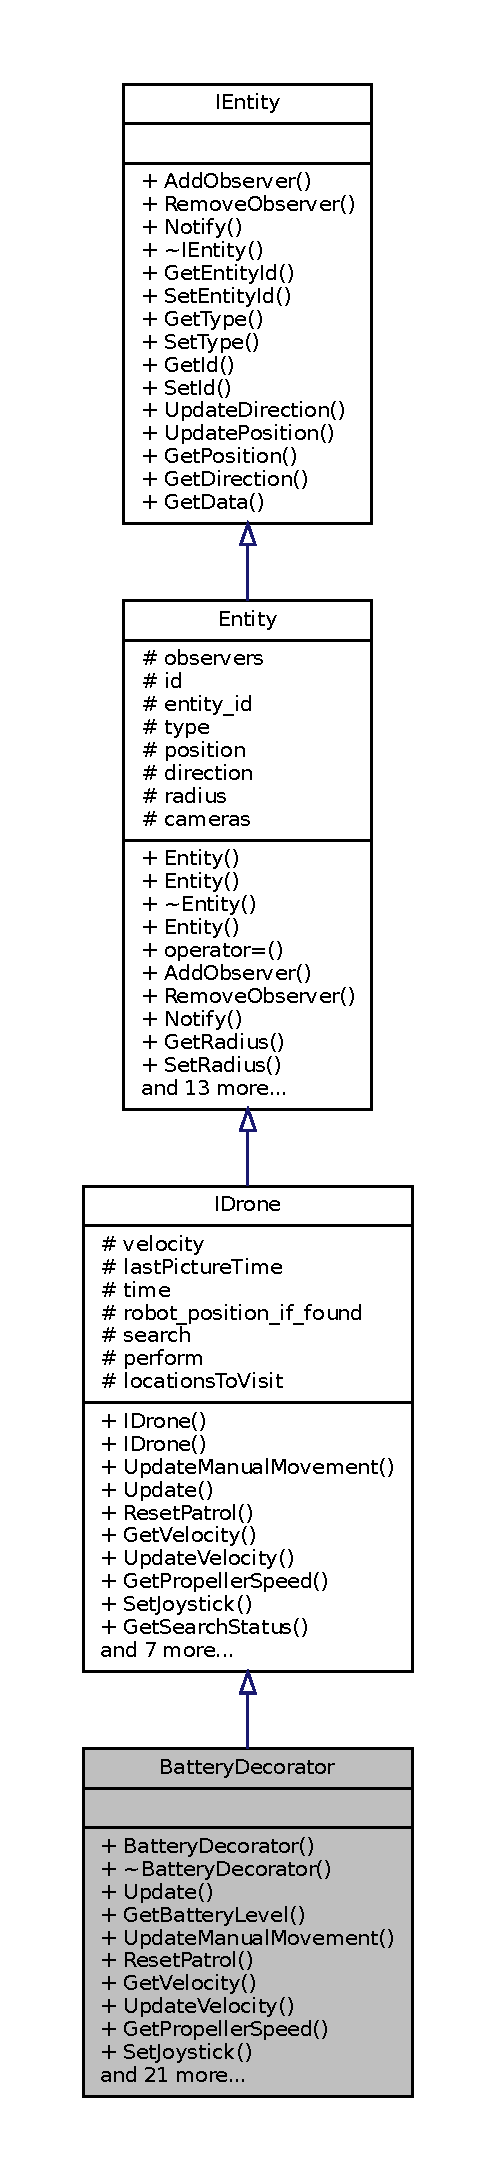
\includegraphics[height=550pt]{classBatteryDecorator__inherit__graph}
\end{center}
\end{figure}


Collaboration diagram for Battery\+Decorator\+:\nopagebreak
\begin{figure}[H]
\begin{center}
\leavevmode
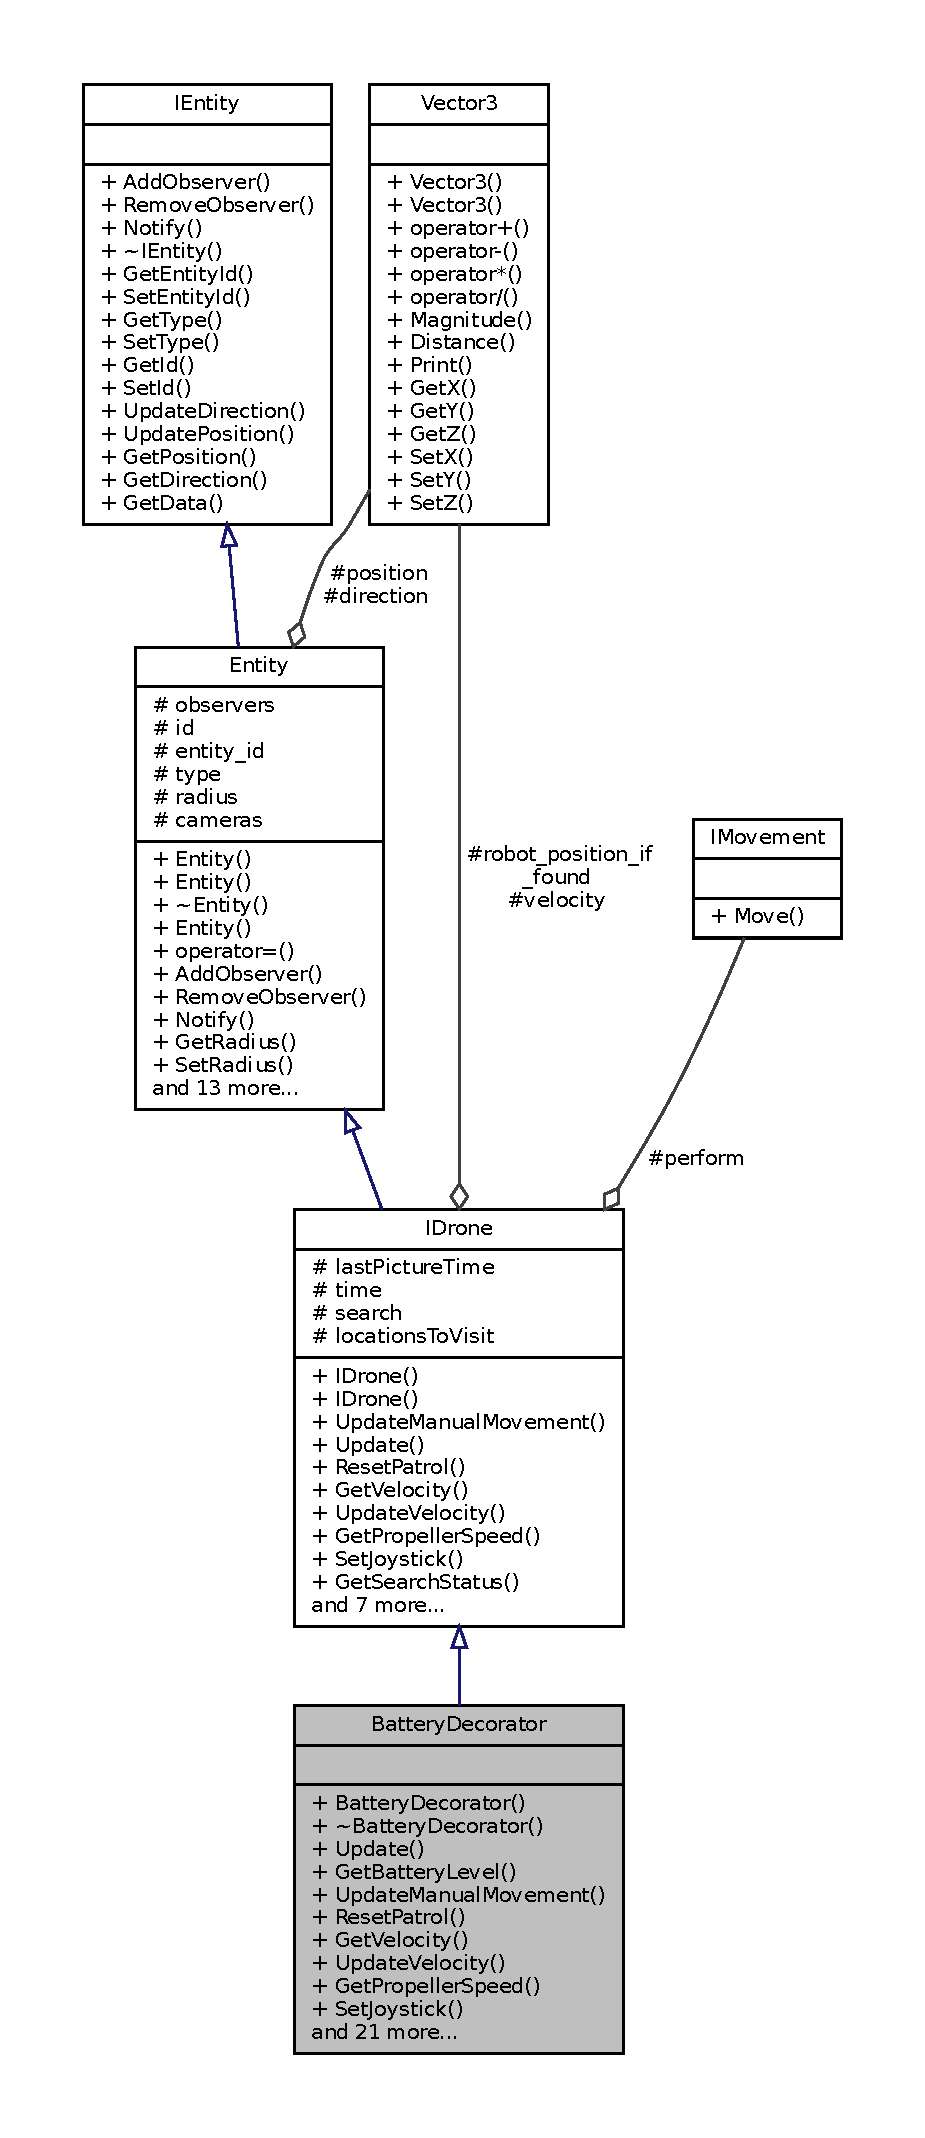
\includegraphics[height=550pt]{classBatteryDecorator__coll__graph}
\end{center}
\end{figure}
\subsection*{Public Member Functions}
\begin{DoxyCompactItemize}
\item 
\hyperlink{classBatteryDecorator_a4bf9b42cd8a12a058107911c6a8ce2cf}{Battery\+Decorator} (\hyperlink{classIDrone}{I\+Drone} $\ast$drone\+\_\+obj, double level=1000)
\begin{DoxyCompactList}\small\item\em constructor, sets battery level \end{DoxyCompactList}\item 
\mbox{\Hypertarget{classBatteryDecorator_a0036d03d5fc869eb39e55734d1e5bb87}\label{classBatteryDecorator_a0036d03d5fc869eb39e55734d1e5bb87}} 
\hyperlink{classBatteryDecorator_a0036d03d5fc869eb39e55734d1e5bb87}{$\sim$\+Battery\+Decorator} ()
\begin{DoxyCompactList}\small\item\em A destructor for all \hyperlink{classBatteryDecorator}{Battery\+Decorator} instances. \end{DoxyCompactList}\item 
void \hyperlink{classBatteryDecorator_a92ea38b63e41d61d7392cb58a53fa8d9}{Update} (double dt)
\begin{DoxyCompactList}\small\item\em Calculates the new position of the drone based on Euler´s integration. \end{DoxyCompactList}\item 
\mbox{\Hypertarget{classBatteryDecorator_abf1c1655d13fbaae30cc31b56dcb18c7}\label{classBatteryDecorator_abf1c1655d13fbaae30cc31b56dcb18c7}} 
float \hyperlink{classBatteryDecorator_abf1c1655d13fbaae30cc31b56dcb18c7}{Get\+Battery\+Level} ()
\begin{DoxyCompactList}\small\item\em Returns the battery level of the drone. \end{DoxyCompactList}\item 
virtual void \hyperlink{classBatteryDecorator_a45babf9bc5484acb95701d361e89de9b}{Update\+Manual\+Movement} (double dt)
\begin{DoxyCompactList}\small\item\em Moves based on keyboard inputs. \end{DoxyCompactList}\item 
\mbox{\Hypertarget{classBatteryDecorator_a36bd4557608043a6934b8c5d73ad511e}\label{classBatteryDecorator_a36bd4557608043a6934b8c5d73ad511e}} 
virtual void \hyperlink{classBatteryDecorator_a36bd4557608043a6934b8c5d73ad511e}{Reset\+Patrol} ()
\begin{DoxyCompactList}\small\item\em Calculates the new patrol movement if we are still searching for the robot and have switch between manual and automatic movement. \end{DoxyCompactList}\item 
virtual \hyperlink{classVector3}{Vector3} \hyperlink{classBatteryDecorator_a978565b772172669437ffec923349f32}{Get\+Velocity} () const
\begin{DoxyCompactList}\small\item\em getter for the velocity of the drone \end{DoxyCompactList}\item 
virtual void \hyperlink{classBatteryDecorator_aad635fd483288cdcc46892da5265ca49}{Update\+Velocity} (const \hyperlink{classVector3}{Vector3} \&new\+Dir)
\begin{DoxyCompactList}\small\item\em Updates the velocity of the drone. \end{DoxyCompactList}\item 
virtual double \hyperlink{classBatteryDecorator_a361154605b803347aea2422cae7d0183}{Get\+Propeller\+Speed} (int index)
\begin{DoxyCompactList}\small\item\em getter for the speed of one of the legs of the drone \end{DoxyCompactList}\item 
virtual void \hyperlink{classBatteryDecorator_abb1ece4f26ac33daefd53a56180721eb}{Set\+Joystick} (double x, double y, double z, double rotate)
\begin{DoxyCompactList}\small\item\em setter for the direction of the drone based on manual movement \end{DoxyCompactList}\item 
virtual bool \hyperlink{classBatteryDecorator_aa0358ef7a9aee0f4942d32ad15ce4675}{Get\+Search\+Status} () const
\begin{DoxyCompactList}\small\item\em getter for the state of drone´s search (robot found or Not) \end{DoxyCompactList}\item 
virtual void \hyperlink{classBatteryDecorator_a41d8c8512cf82484120a9f3f951c4c2b}{Set\+Search\+Status} (bool status)
\begin{DoxyCompactList}\small\item\em setter for the state of drone´s search (robot found or Not) \end{DoxyCompactList}\item 
virtual float \hyperlink{classBatteryDecorator_a661b3722c37ce7d9690e50724eac863e}{Get\+Last\+Picture\+Time} () const
\begin{DoxyCompactList}\small\item\em getter for the last time drone took a pic \end{DoxyCompactList}\item 
virtual void \hyperlink{classBatteryDecorator_abcaad479f82c6b8fcef4b511fb702d61}{Set\+Last\+Picture\+Time} (float time\+Pic)
\begin{DoxyCompactList}\small\item\em setter for the last time drone took a pic \end{DoxyCompactList}\item 
virtual float \hyperlink{classBatteryDecorator_a87cb6d468b6cd418775b4e01308fc0bf}{Get\+Time} () const
\begin{DoxyCompactList}\small\item\em getter for the time elapsed \end{DoxyCompactList}\item 
virtual void \hyperlink{classBatteryDecorator_abf7e2a2b4634330de27e7072236ffc5f}{Set\+Time} (float t)
\begin{DoxyCompactList}\small\item\em setter for the time elapsed \end{DoxyCompactList}\item 
int \hyperlink{classBatteryDecorator_a0a9d1aedcbbff75c0a88612cb4604fb3}{Get\+Id} ()
\begin{DoxyCompactList}\small\item\em This will return an integer that represents the command in which the object was created. \end{DoxyCompactList}\item 
int \hyperlink{classBatteryDecorator_a38fb935ea609ef4e38ebb50e70200a43}{Get\+Entity\+Id} ()
\begin{DoxyCompactList}\small\item\em This will return the \hyperlink{classEntity}{Entity} Id, meaning the type of object (0 represents a drone) \end{DoxyCompactList}\item 
std\+::string \hyperlink{classBatteryDecorator_a606b100a52321dee5c36fe3942f8c396}{Get\+Type} ()
\begin{DoxyCompactList}\small\item\em This will return a string representing object type \char`\"{}drone\char`\"{}, \char`\"{}hospital\char`\"{}... \end{DoxyCompactList}\item 
void \hyperlink{classBatteryDecorator_aafe8d17f609556cfcb5537e38adc66f2}{Set\+Id} (int id2)
\begin{DoxyCompactList}\small\item\em This will set the command \# in which the object was created. \end{DoxyCompactList}\item 
void \hyperlink{classBatteryDecorator_a59bc5191357fdeb9a52ee6121d79b12d}{Set\+Entity\+Id} (int id2)
\begin{DoxyCompactList}\small\item\em This will set the \hyperlink{classEntity}{Entity} Id, meaning the type of object (0 represents a drone) \end{DoxyCompactList}\item 
void \hyperlink{classBatteryDecorator_a815d1943eef8e5f147158a043fe02825}{Set\+Type} (std\+::string \&name)
\begin{DoxyCompactList}\small\item\em This will set the object type \char`\"{}drone\char`\"{}, \char`\"{}hospital\char`\"{}... \end{DoxyCompactList}\item 
void \hyperlink{classBatteryDecorator_a42dfc0dc6cd4423f8113609ea7f5e938}{Update\+Direction} (const \hyperlink{classVector3}{Vector3} \&new\+Dir)
\begin{DoxyCompactList}\small\item\em Updates the direction of the entity. \end{DoxyCompactList}\item 
void \hyperlink{classBatteryDecorator_a7c338ca278f03c5c0fcea39885fc7d43}{Update\+Position} (const \hyperlink{classVector3}{Vector3} \&new\+Dir)
\begin{DoxyCompactList}\small\item\em Updates the position of the entity. \end{DoxyCompactList}\item 
\hyperlink{classVector3}{Vector3} \hyperlink{classBatteryDecorator_aaf2487adf2d58e855268877427cf5ba9}{Get\+Position} () const
\begin{DoxyCompactList}\small\item\em getter for entity position \end{DoxyCompactList}\item 
\hyperlink{classVector3}{Vector3} \hyperlink{classBatteryDecorator_a8487174df54456fe29406927f0542720}{Get\+Direction} () const
\begin{DoxyCompactList}\small\item\em getter for entity direction \end{DoxyCompactList}\item 
void \hyperlink{classBatteryDecorator_a25470bba4af4e6c112a858584a38fcdd}{Add\+Camera} (\hyperlink{classCamera}{Camera} $\ast$new\+\_\+camera)
\begin{DoxyCompactList}\small\item\em Function that will add a camera to the vector of cameras of the entity. \end{DoxyCompactList}\item 
\hyperlink{classCamera}{Camera} $\ast$ \hyperlink{classBatteryDecorator_ad65baa2cd098b990a49bdff7c0fde62c}{Get\+Camera} (int idx)
\begin{DoxyCompactList}\small\item\em Get the idx camera from the cameras of the entity. \end{DoxyCompactList}\item 
std\+::string \hyperlink{classBatteryDecorator_a47475a9179285e30e8c18316cebdac9f}{Get\+Data} (float dt)
\begin{DoxyCompactList}\small\item\em A method to get the pertinent data of an \hyperlink{classEntity}{Entity} to be written to C\+SV file. \end{DoxyCompactList}\item 
\hyperlink{classVector3}{Vector3} \hyperlink{classBatteryDecorator_ac9f7223d439db341e9765ea3d5584f4e}{Get\+Robot\+Pos} () const
\begin{DoxyCompactList}\small\item\em A method to get the robot x y z position. \end{DoxyCompactList}\item 
void \hyperlink{classBatteryDecorator_a183e98816461760d499366e112e5d0a6}{Set\+Robot\+Pos} (\hyperlink{classVector3}{Vector3} pos)
\begin{DoxyCompactList}\small\item\em A method to set the robot x y z position. \end{DoxyCompactList}\end{DoxyCompactItemize}
\subsection*{Additional Inherited Members}


\subsection{Constructor \& Destructor Documentation}
\mbox{\Hypertarget{classBatteryDecorator_a4bf9b42cd8a12a058107911c6a8ce2cf}\label{classBatteryDecorator_a4bf9b42cd8a12a058107911c6a8ce2cf}} 
\index{Battery\+Decorator@{Battery\+Decorator}!Battery\+Decorator@{Battery\+Decorator}}
\index{Battery\+Decorator@{Battery\+Decorator}!Battery\+Decorator@{Battery\+Decorator}}
\subsubsection{\texorpdfstring{Battery\+Decorator()}{BatteryDecorator()}}
{\footnotesize\ttfamily Battery\+Decorator\+::\+Battery\+Decorator (\begin{DoxyParamCaption}\item[{\hyperlink{classIDrone}{I\+Drone} $\ast$}]{drone\+\_\+obj,  }\item[{double}]{level = {\ttfamily 1000} }\end{DoxyParamCaption})}



constructor, sets battery level 


\begin{DoxyParams}[1]{Parameters}
\mbox{\tt in}  & {\em drone\+\_\+obj} & I\+Drone$\ast$ base drone to be decorated \\
\hline
\mbox{\tt in}  & {\em level} & double amount of battery that the drone starts with \\
\hline
\end{DoxyParams}


\subsection{Member Function Documentation}
\mbox{\Hypertarget{classBatteryDecorator_a25470bba4af4e6c112a858584a38fcdd}\label{classBatteryDecorator_a25470bba4af4e6c112a858584a38fcdd}} 
\index{Battery\+Decorator@{Battery\+Decorator}!Add\+Camera@{Add\+Camera}}
\index{Add\+Camera@{Add\+Camera}!Battery\+Decorator@{Battery\+Decorator}}
\subsubsection{\texorpdfstring{Add\+Camera()}{AddCamera()}}
{\footnotesize\ttfamily void Battery\+Decorator\+::\+Add\+Camera (\begin{DoxyParamCaption}\item[{\hyperlink{classCamera}{Camera} $\ast$}]{new\+\_\+camera }\end{DoxyParamCaption})\hspace{0.3cm}{\ttfamily [virtual]}}



Function that will add a camera to the vector of cameras of the entity. 


\begin{DoxyParams}[1]{Parameters}
\mbox{\tt in}  & {\em new\+\_\+camera} & New camera object to be added to the vector of cameras of the entity \\
\hline
\end{DoxyParams}


Reimplemented from \hyperlink{classEntity_a9f3c739a3ef623a9febc7801270ba719}{Entity}.

\mbox{\Hypertarget{classBatteryDecorator_ad65baa2cd098b990a49bdff7c0fde62c}\label{classBatteryDecorator_ad65baa2cd098b990a49bdff7c0fde62c}} 
\index{Battery\+Decorator@{Battery\+Decorator}!Get\+Camera@{Get\+Camera}}
\index{Get\+Camera@{Get\+Camera}!Battery\+Decorator@{Battery\+Decorator}}
\subsubsection{\texorpdfstring{Get\+Camera()}{GetCamera()}}
{\footnotesize\ttfamily \hyperlink{classCamera}{Camera} $\ast$ Battery\+Decorator\+::\+Get\+Camera (\begin{DoxyParamCaption}\item[{int}]{idx }\end{DoxyParamCaption})\hspace{0.3cm}{\ttfamily [virtual]}}



Get the idx camera from the cameras of the entity. 


\begin{DoxyParams}[1]{Parameters}
\mbox{\tt in}  & {\em idx} & integer representing the camera you want to get\\
\hline
\end{DoxyParams}
\begin{DoxyReturn}{Returns}
\hyperlink{classCamera}{Camera} object pointer 
\end{DoxyReturn}


Reimplemented from \hyperlink{classEntity_ae09d3e79d0d14c2990b1da52d2268399}{Entity}.

\mbox{\Hypertarget{classBatteryDecorator_a47475a9179285e30e8c18316cebdac9f}\label{classBatteryDecorator_a47475a9179285e30e8c18316cebdac9f}} 
\index{Battery\+Decorator@{Battery\+Decorator}!Get\+Data@{Get\+Data}}
\index{Get\+Data@{Get\+Data}!Battery\+Decorator@{Battery\+Decorator}}
\subsubsection{\texorpdfstring{Get\+Data()}{GetData()}}
{\footnotesize\ttfamily std\+::string Battery\+Decorator\+::\+Get\+Data (\begin{DoxyParamCaption}\item[{float}]{dt }\end{DoxyParamCaption})\hspace{0.3cm}{\ttfamily [virtual]}}



A method to get the pertinent data of an \hyperlink{classEntity}{Entity} to be written to C\+SV file. 


\begin{DoxyParams}[1]{Parameters}
\mbox{\tt in}  & {\em dt} & A float representing the change in time since the last update\\
\hline
\end{DoxyParams}
\begin{DoxyReturn}{Returns}
String Returns a string containing the comma separated data to be written to a C\+SV file. 
\end{DoxyReturn}


Implements \hyperlink{classIEntity_a4d9355e68c6be349f57dc67fc1c036ba}{I\+Entity}.

\mbox{\Hypertarget{classBatteryDecorator_a8487174df54456fe29406927f0542720}\label{classBatteryDecorator_a8487174df54456fe29406927f0542720}} 
\index{Battery\+Decorator@{Battery\+Decorator}!Get\+Direction@{Get\+Direction}}
\index{Get\+Direction@{Get\+Direction}!Battery\+Decorator@{Battery\+Decorator}}
\subsubsection{\texorpdfstring{Get\+Direction()}{GetDirection()}}
{\footnotesize\ttfamily \hyperlink{classVector3}{Vector3} Battery\+Decorator\+::\+Get\+Direction (\begin{DoxyParamCaption}{ }\end{DoxyParamCaption}) const\hspace{0.3cm}{\ttfamily [virtual]}}



getter for entity direction 

\begin{DoxyReturn}{Returns}
\hyperlink{classVector3}{Vector3} object representing the entity direction 
\end{DoxyReturn}


Implements \hyperlink{classIEntity_aa99a8fef8b22195a5113c38ef51f086d}{I\+Entity}.

\mbox{\Hypertarget{classBatteryDecorator_a38fb935ea609ef4e38ebb50e70200a43}\label{classBatteryDecorator_a38fb935ea609ef4e38ebb50e70200a43}} 
\index{Battery\+Decorator@{Battery\+Decorator}!Get\+Entity\+Id@{Get\+Entity\+Id}}
\index{Get\+Entity\+Id@{Get\+Entity\+Id}!Battery\+Decorator@{Battery\+Decorator}}
\subsubsection{\texorpdfstring{Get\+Entity\+Id()}{GetEntityId()}}
{\footnotesize\ttfamily int Battery\+Decorator\+::\+Get\+Entity\+Id (\begin{DoxyParamCaption}{ }\end{DoxyParamCaption})\hspace{0.3cm}{\ttfamily [virtual]}}



This will return the \hyperlink{classEntity}{Entity} Id, meaning the type of object (0 represents a drone) 

\begin{DoxyReturn}{Returns}
integer representing the type of object of the entity 
\end{DoxyReturn}


Implements \hyperlink{classIEntity_a4359ee47413fa0b2940b3b0336e13861}{I\+Entity}.

\mbox{\Hypertarget{classBatteryDecorator_a0a9d1aedcbbff75c0a88612cb4604fb3}\label{classBatteryDecorator_a0a9d1aedcbbff75c0a88612cb4604fb3}} 
\index{Battery\+Decorator@{Battery\+Decorator}!Get\+Id@{Get\+Id}}
\index{Get\+Id@{Get\+Id}!Battery\+Decorator@{Battery\+Decorator}}
\subsubsection{\texorpdfstring{Get\+Id()}{GetId()}}
{\footnotesize\ttfamily int Battery\+Decorator\+::\+Get\+Id (\begin{DoxyParamCaption}{ }\end{DoxyParamCaption})\hspace{0.3cm}{\ttfamily [virtual]}}



This will return an integer that represents the command in which the object was created. 

\begin{DoxyReturn}{Returns}
id representing the command number 
\end{DoxyReturn}


Implements \hyperlink{classIEntity_ac3d60cc2fab1ccb61c1be92373e636d9}{I\+Entity}.

\mbox{\Hypertarget{classBatteryDecorator_a661b3722c37ce7d9690e50724eac863e}\label{classBatteryDecorator_a661b3722c37ce7d9690e50724eac863e}} 
\index{Battery\+Decorator@{Battery\+Decorator}!Get\+Last\+Picture\+Time@{Get\+Last\+Picture\+Time}}
\index{Get\+Last\+Picture\+Time@{Get\+Last\+Picture\+Time}!Battery\+Decorator@{Battery\+Decorator}}
\subsubsection{\texorpdfstring{Get\+Last\+Picture\+Time()}{GetLastPictureTime()}}
{\footnotesize\ttfamily float Battery\+Decorator\+::\+Get\+Last\+Picture\+Time (\begin{DoxyParamCaption}{ }\end{DoxyParamCaption}) const\hspace{0.3cm}{\ttfamily [virtual]}}



getter for the last time drone took a pic 

\begin{DoxyReturn}{Returns}
float representing time elapsed since that picture 
\end{DoxyReturn}


Implements \hyperlink{classIDrone_a112d19971ac7d94dba9e2f25ad667c0d}{I\+Drone}.

\mbox{\Hypertarget{classBatteryDecorator_aaf2487adf2d58e855268877427cf5ba9}\label{classBatteryDecorator_aaf2487adf2d58e855268877427cf5ba9}} 
\index{Battery\+Decorator@{Battery\+Decorator}!Get\+Position@{Get\+Position}}
\index{Get\+Position@{Get\+Position}!Battery\+Decorator@{Battery\+Decorator}}
\subsubsection{\texorpdfstring{Get\+Position()}{GetPosition()}}
{\footnotesize\ttfamily \hyperlink{classVector3}{Vector3} Battery\+Decorator\+::\+Get\+Position (\begin{DoxyParamCaption}{ }\end{DoxyParamCaption}) const\hspace{0.3cm}{\ttfamily [virtual]}}



getter for entity position 

\begin{DoxyReturn}{Returns}
\hyperlink{classVector3}{Vector3} object representing the entity position 
\end{DoxyReturn}


Implements \hyperlink{classIEntity_a9bc32587aab91761fc0e718612498199}{I\+Entity}.

\mbox{\Hypertarget{classBatteryDecorator_a361154605b803347aea2422cae7d0183}\label{classBatteryDecorator_a361154605b803347aea2422cae7d0183}} 
\index{Battery\+Decorator@{Battery\+Decorator}!Get\+Propeller\+Speed@{Get\+Propeller\+Speed}}
\index{Get\+Propeller\+Speed@{Get\+Propeller\+Speed}!Battery\+Decorator@{Battery\+Decorator}}
\subsubsection{\texorpdfstring{Get\+Propeller\+Speed()}{GetPropellerSpeed()}}
{\footnotesize\ttfamily double Battery\+Decorator\+::\+Get\+Propeller\+Speed (\begin{DoxyParamCaption}\item[{int}]{index }\end{DoxyParamCaption})\hspace{0.3cm}{\ttfamily [virtual]}}



getter for the speed of one of the legs of the drone 

\begin{DoxyReturn}{Returns}
double representing the speed of the index propeller 
\end{DoxyReturn}


Implements \hyperlink{classIDrone_a60a9a7eb90bf13100d66cb47b99830ed}{I\+Drone}.

\mbox{\Hypertarget{classBatteryDecorator_ac9f7223d439db341e9765ea3d5584f4e}\label{classBatteryDecorator_ac9f7223d439db341e9765ea3d5584f4e}} 
\index{Battery\+Decorator@{Battery\+Decorator}!Get\+Robot\+Pos@{Get\+Robot\+Pos}}
\index{Get\+Robot\+Pos@{Get\+Robot\+Pos}!Battery\+Decorator@{Battery\+Decorator}}
\subsubsection{\texorpdfstring{Get\+Robot\+Pos()}{GetRobotPos()}}
{\footnotesize\ttfamily \hyperlink{classVector3}{Vector3} Battery\+Decorator\+::\+Get\+Robot\+Pos (\begin{DoxyParamCaption}{ }\end{DoxyParamCaption}) const\hspace{0.3cm}{\ttfamily [virtual]}}



A method to get the robot x y z position. 

\begin{DoxyReturn}{Returns}
Vector representing position where robot found 
\end{DoxyReturn}


Implements \hyperlink{classIDrone_a1c3f5e712a97625c74c35952b930d68d}{I\+Drone}.

\mbox{\Hypertarget{classBatteryDecorator_aa0358ef7a9aee0f4942d32ad15ce4675}\label{classBatteryDecorator_aa0358ef7a9aee0f4942d32ad15ce4675}} 
\index{Battery\+Decorator@{Battery\+Decorator}!Get\+Search\+Status@{Get\+Search\+Status}}
\index{Get\+Search\+Status@{Get\+Search\+Status}!Battery\+Decorator@{Battery\+Decorator}}
\subsubsection{\texorpdfstring{Get\+Search\+Status()}{GetSearchStatus()}}
{\footnotesize\ttfamily bool Battery\+Decorator\+::\+Get\+Search\+Status (\begin{DoxyParamCaption}{ }\end{DoxyParamCaption}) const\hspace{0.3cm}{\ttfamily [virtual]}}



getter for the state of drone´s search (robot found or Not) 

\begin{DoxyReturn}{Returns}
boolean true if we have found robot and are moving torwards it, false otherwise 
\end{DoxyReturn}


Implements \hyperlink{classIDrone_aed9abde2152408ef3483da57f24c4006}{I\+Drone}.

\mbox{\Hypertarget{classBatteryDecorator_a87cb6d468b6cd418775b4e01308fc0bf}\label{classBatteryDecorator_a87cb6d468b6cd418775b4e01308fc0bf}} 
\index{Battery\+Decorator@{Battery\+Decorator}!Get\+Time@{Get\+Time}}
\index{Get\+Time@{Get\+Time}!Battery\+Decorator@{Battery\+Decorator}}
\subsubsection{\texorpdfstring{Get\+Time()}{GetTime()}}
{\footnotesize\ttfamily float Battery\+Decorator\+::\+Get\+Time (\begin{DoxyParamCaption}{ }\end{DoxyParamCaption}) const\hspace{0.3cm}{\ttfamily [virtual]}}



getter for the time elapsed 

\begin{DoxyReturn}{Returns}
float representing time elapsed (sum of updates dt´s) 
\end{DoxyReturn}


Implements \hyperlink{classIDrone_a18809d1b0626ba66984ef3a91ffb644c}{I\+Drone}.

\mbox{\Hypertarget{classBatteryDecorator_a606b100a52321dee5c36fe3942f8c396}\label{classBatteryDecorator_a606b100a52321dee5c36fe3942f8c396}} 
\index{Battery\+Decorator@{Battery\+Decorator}!Get\+Type@{Get\+Type}}
\index{Get\+Type@{Get\+Type}!Battery\+Decorator@{Battery\+Decorator}}
\subsubsection{\texorpdfstring{Get\+Type()}{GetType()}}
{\footnotesize\ttfamily std\+::string Battery\+Decorator\+::\+Get\+Type (\begin{DoxyParamCaption}{ }\end{DoxyParamCaption})\hspace{0.3cm}{\ttfamily [virtual]}}



This will return a string representing object type \char`\"{}drone\char`\"{}, \char`\"{}hospital\char`\"{}... 

\begin{DoxyReturn}{Returns}
string representing the type of object of the entity 
\end{DoxyReturn}


Implements \hyperlink{classIEntity_ac494bb9712d5a03495a1a95afdbd7153}{I\+Entity}.

\mbox{\Hypertarget{classBatteryDecorator_a978565b772172669437ffec923349f32}\label{classBatteryDecorator_a978565b772172669437ffec923349f32}} 
\index{Battery\+Decorator@{Battery\+Decorator}!Get\+Velocity@{Get\+Velocity}}
\index{Get\+Velocity@{Get\+Velocity}!Battery\+Decorator@{Battery\+Decorator}}
\subsubsection{\texorpdfstring{Get\+Velocity()}{GetVelocity()}}
{\footnotesize\ttfamily \hyperlink{classVector3}{Vector3} Battery\+Decorator\+::\+Get\+Velocity (\begin{DoxyParamCaption}{ }\end{DoxyParamCaption}) const\hspace{0.3cm}{\ttfamily [virtual]}}



getter for the velocity of the drone 

\begin{DoxyReturn}{Returns}
vector3 representing the velocity of the drone 
\end{DoxyReturn}


Implements \hyperlink{classIDrone_abad6c0adb60d6deceb13f30687fed57b}{I\+Drone}.

\mbox{\Hypertarget{classBatteryDecorator_a59bc5191357fdeb9a52ee6121d79b12d}\label{classBatteryDecorator_a59bc5191357fdeb9a52ee6121d79b12d}} 
\index{Battery\+Decorator@{Battery\+Decorator}!Set\+Entity\+Id@{Set\+Entity\+Id}}
\index{Set\+Entity\+Id@{Set\+Entity\+Id}!Battery\+Decorator@{Battery\+Decorator}}
\subsubsection{\texorpdfstring{Set\+Entity\+Id()}{SetEntityId()}}
{\footnotesize\ttfamily void Battery\+Decorator\+::\+Set\+Entity\+Id (\begin{DoxyParamCaption}\item[{int}]{id2 }\end{DoxyParamCaption})\hspace{0.3cm}{\ttfamily [virtual]}}



This will set the \hyperlink{classEntity}{Entity} Id, meaning the type of object (0 represents a drone) 


\begin{DoxyParams}[1]{Parameters}
\mbox{\tt in}  & {\em id2} & integer representing the type of object of the entity \\
\hline
\end{DoxyParams}


Implements \hyperlink{classIEntity_a3a830862181cb0548d2aca83d908263e}{I\+Entity}.

\mbox{\Hypertarget{classBatteryDecorator_aafe8d17f609556cfcb5537e38adc66f2}\label{classBatteryDecorator_aafe8d17f609556cfcb5537e38adc66f2}} 
\index{Battery\+Decorator@{Battery\+Decorator}!Set\+Id@{Set\+Id}}
\index{Set\+Id@{Set\+Id}!Battery\+Decorator@{Battery\+Decorator}}
\subsubsection{\texorpdfstring{Set\+Id()}{SetId()}}
{\footnotesize\ttfamily void Battery\+Decorator\+::\+Set\+Id (\begin{DoxyParamCaption}\item[{int}]{id2 }\end{DoxyParamCaption})\hspace{0.3cm}{\ttfamily [virtual]}}



This will set the command \# in which the object was created. 


\begin{DoxyParams}[1]{Parameters}
\mbox{\tt in}  & {\em id2} & the command number as an integer \\
\hline
\end{DoxyParams}


Implements \hyperlink{classIEntity_a8c6af682e07f569ba2f164d214295c67}{I\+Entity}.

\mbox{\Hypertarget{classBatteryDecorator_abb1ece4f26ac33daefd53a56180721eb}\label{classBatteryDecorator_abb1ece4f26ac33daefd53a56180721eb}} 
\index{Battery\+Decorator@{Battery\+Decorator}!Set\+Joystick@{Set\+Joystick}}
\index{Set\+Joystick@{Set\+Joystick}!Battery\+Decorator@{Battery\+Decorator}}
\subsubsection{\texorpdfstring{Set\+Joystick()}{SetJoystick()}}
{\footnotesize\ttfamily void Battery\+Decorator\+::\+Set\+Joystick (\begin{DoxyParamCaption}\item[{double}]{x,  }\item[{double}]{y,  }\item[{double}]{z,  }\item[{double}]{rotate }\end{DoxyParamCaption})\hspace{0.3cm}{\ttfamily [virtual]}}



setter for the direction of the drone based on manual movement 


\begin{DoxyParams}[1]{Parameters}
\mbox{\tt in}  & {\em x} & double representing the direction on the x direction \\
\hline
\mbox{\tt in}  & {\em y} & double representing the direction on the y direction \\
\hline
\mbox{\tt in}  & {\em z} & double representing the direction on the z direction \\
\hline
\mbox{\tt in}  & {\em rotate} & double representing the rotation value of drone \\
\hline
\end{DoxyParams}


Implements \hyperlink{classIDrone_a8414edd320f25869fb04a880eae0d554}{I\+Drone}.

\mbox{\Hypertarget{classBatteryDecorator_abcaad479f82c6b8fcef4b511fb702d61}\label{classBatteryDecorator_abcaad479f82c6b8fcef4b511fb702d61}} 
\index{Battery\+Decorator@{Battery\+Decorator}!Set\+Last\+Picture\+Time@{Set\+Last\+Picture\+Time}}
\index{Set\+Last\+Picture\+Time@{Set\+Last\+Picture\+Time}!Battery\+Decorator@{Battery\+Decorator}}
\subsubsection{\texorpdfstring{Set\+Last\+Picture\+Time()}{SetLastPictureTime()}}
{\footnotesize\ttfamily void Battery\+Decorator\+::\+Set\+Last\+Picture\+Time (\begin{DoxyParamCaption}\item[{float}]{time\+Pic }\end{DoxyParamCaption})\hspace{0.3cm}{\ttfamily [virtual]}}



setter for the last time drone took a pic 


\begin{DoxyParams}[1]{Parameters}
\mbox{\tt in}  & {\em time\+Pic} & float representing time since last\+Picture \\
\hline
\end{DoxyParams}


Implements \hyperlink{classIDrone_aace45f6d9a77bfc8c61bd0ffc30a3b8e}{I\+Drone}.

\mbox{\Hypertarget{classBatteryDecorator_a183e98816461760d499366e112e5d0a6}\label{classBatteryDecorator_a183e98816461760d499366e112e5d0a6}} 
\index{Battery\+Decorator@{Battery\+Decorator}!Set\+Robot\+Pos@{Set\+Robot\+Pos}}
\index{Set\+Robot\+Pos@{Set\+Robot\+Pos}!Battery\+Decorator@{Battery\+Decorator}}
\subsubsection{\texorpdfstring{Set\+Robot\+Pos()}{SetRobotPos()}}
{\footnotesize\ttfamily void Battery\+Decorator\+::\+Set\+Robot\+Pos (\begin{DoxyParamCaption}\item[{\hyperlink{classVector3}{Vector3}}]{pos }\end{DoxyParamCaption})\hspace{0.3cm}{\ttfamily [virtual]}}



A method to set the robot x y z position. 


\begin{DoxyParams}[1]{Parameters}
\mbox{\tt in}  & {\em pos} & Vector representing position where robot found \\
\hline
\end{DoxyParams}


Implements \hyperlink{classIDrone_a5851e679bf3c915e93165377cb5c8815}{I\+Drone}.

\mbox{\Hypertarget{classBatteryDecorator_a41d8c8512cf82484120a9f3f951c4c2b}\label{classBatteryDecorator_a41d8c8512cf82484120a9f3f951c4c2b}} 
\index{Battery\+Decorator@{Battery\+Decorator}!Set\+Search\+Status@{Set\+Search\+Status}}
\index{Set\+Search\+Status@{Set\+Search\+Status}!Battery\+Decorator@{Battery\+Decorator}}
\subsubsection{\texorpdfstring{Set\+Search\+Status()}{SetSearchStatus()}}
{\footnotesize\ttfamily void Battery\+Decorator\+::\+Set\+Search\+Status (\begin{DoxyParamCaption}\item[{bool}]{status }\end{DoxyParamCaption})\hspace{0.3cm}{\ttfamily [virtual]}}



setter for the state of drone´s search (robot found or Not) 


\begin{DoxyParams}[1]{Parameters}
\mbox{\tt in}  & {\em status} & boolean true if we have found robot and are moving torwards it, false otherwise \\
\hline
\end{DoxyParams}


Implements \hyperlink{classIDrone_ac6f580814e7091ea64ecf2a7137b8120}{I\+Drone}.

\mbox{\Hypertarget{classBatteryDecorator_abf7e2a2b4634330de27e7072236ffc5f}\label{classBatteryDecorator_abf7e2a2b4634330de27e7072236ffc5f}} 
\index{Battery\+Decorator@{Battery\+Decorator}!Set\+Time@{Set\+Time}}
\index{Set\+Time@{Set\+Time}!Battery\+Decorator@{Battery\+Decorator}}
\subsubsection{\texorpdfstring{Set\+Time()}{SetTime()}}
{\footnotesize\ttfamily void Battery\+Decorator\+::\+Set\+Time (\begin{DoxyParamCaption}\item[{float}]{t }\end{DoxyParamCaption})\hspace{0.3cm}{\ttfamily [virtual]}}



setter for the time elapsed 


\begin{DoxyParams}[1]{Parameters}
\mbox{\tt in}  & {\em t} & float representing time elapsed (sum of updates dt´s) \\
\hline
\end{DoxyParams}


Implements \hyperlink{classIDrone_a0ca36885fd79fbf2efa3909771218d56}{I\+Drone}.

\mbox{\Hypertarget{classBatteryDecorator_a815d1943eef8e5f147158a043fe02825}\label{classBatteryDecorator_a815d1943eef8e5f147158a043fe02825}} 
\index{Battery\+Decorator@{Battery\+Decorator}!Set\+Type@{Set\+Type}}
\index{Set\+Type@{Set\+Type}!Battery\+Decorator@{Battery\+Decorator}}
\subsubsection{\texorpdfstring{Set\+Type()}{SetType()}}
{\footnotesize\ttfamily void Battery\+Decorator\+::\+Set\+Type (\begin{DoxyParamCaption}\item[{std\+::string \&}]{name }\end{DoxyParamCaption})\hspace{0.3cm}{\ttfamily [virtual]}}



This will set the object type \char`\"{}drone\char`\"{}, \char`\"{}hospital\char`\"{}... 


\begin{DoxyParams}[1]{Parameters}
\mbox{\tt in}  & {\em name} & string representing the type of object of the entity \\
\hline
\end{DoxyParams}


Implements \hyperlink{classIEntity_a49b3c54f94a93d4a9f96527ffb8982f5}{I\+Entity}.

\mbox{\Hypertarget{classBatteryDecorator_a92ea38b63e41d61d7392cb58a53fa8d9}\label{classBatteryDecorator_a92ea38b63e41d61d7392cb58a53fa8d9}} 
\index{Battery\+Decorator@{Battery\+Decorator}!Update@{Update}}
\index{Update@{Update}!Battery\+Decorator@{Battery\+Decorator}}
\subsubsection{\texorpdfstring{Update()}{Update()}}
{\footnotesize\ttfamily void Battery\+Decorator\+::\+Update (\begin{DoxyParamCaption}\item[{double}]{dt }\end{DoxyParamCaption})\hspace{0.3cm}{\ttfamily [virtual]}}



Calculates the new position of the drone based on Euler´s integration. 


\begin{DoxyParams}[1]{Parameters}
\mbox{\tt in}  & {\em dt} & period of time it has elapsed since last update \\
\hline
\end{DoxyParams}


Implements \hyperlink{classIDrone_a6d840d60cda9a985b94af42ef54520b7}{I\+Drone}.

\mbox{\Hypertarget{classBatteryDecorator_a42dfc0dc6cd4423f8113609ea7f5e938}\label{classBatteryDecorator_a42dfc0dc6cd4423f8113609ea7f5e938}} 
\index{Battery\+Decorator@{Battery\+Decorator}!Update\+Direction@{Update\+Direction}}
\index{Update\+Direction@{Update\+Direction}!Battery\+Decorator@{Battery\+Decorator}}
\subsubsection{\texorpdfstring{Update\+Direction()}{UpdateDirection()}}
{\footnotesize\ttfamily void Battery\+Decorator\+::\+Update\+Direction (\begin{DoxyParamCaption}\item[{const \hyperlink{classVector3}{Vector3} \&}]{new\+Dir }\end{DoxyParamCaption})\hspace{0.3cm}{\ttfamily [virtual]}}



Updates the direction of the entity. 


\begin{DoxyParams}[1]{Parameters}
\mbox{\tt in}  & {\em new\+Dir} & vector3 representing the new direction of the object \\
\hline
\end{DoxyParams}


Implements \hyperlink{classIEntity_af24054e349dcdaea31a778427a34495d}{I\+Entity}.

\mbox{\Hypertarget{classBatteryDecorator_a45babf9bc5484acb95701d361e89de9b}\label{classBatteryDecorator_a45babf9bc5484acb95701d361e89de9b}} 
\index{Battery\+Decorator@{Battery\+Decorator}!Update\+Manual\+Movement@{Update\+Manual\+Movement}}
\index{Update\+Manual\+Movement@{Update\+Manual\+Movement}!Battery\+Decorator@{Battery\+Decorator}}
\subsubsection{\texorpdfstring{Update\+Manual\+Movement()}{UpdateManualMovement()}}
{\footnotesize\ttfamily void Battery\+Decorator\+::\+Update\+Manual\+Movement (\begin{DoxyParamCaption}\item[{double}]{dt }\end{DoxyParamCaption})\hspace{0.3cm}{\ttfamily [virtual]}}



Moves based on keyboard inputs. 


\begin{DoxyParams}[1]{Parameters}
\mbox{\tt in}  & {\em dt} & period of time it has elapsed since last update \\
\hline
\end{DoxyParams}


Implements \hyperlink{classIDrone_a82486b4192f6ccf8b3d93fbb9101f2dd}{I\+Drone}.

\mbox{\Hypertarget{classBatteryDecorator_a7c338ca278f03c5c0fcea39885fc7d43}\label{classBatteryDecorator_a7c338ca278f03c5c0fcea39885fc7d43}} 
\index{Battery\+Decorator@{Battery\+Decorator}!Update\+Position@{Update\+Position}}
\index{Update\+Position@{Update\+Position}!Battery\+Decorator@{Battery\+Decorator}}
\subsubsection{\texorpdfstring{Update\+Position()}{UpdatePosition()}}
{\footnotesize\ttfamily void Battery\+Decorator\+::\+Update\+Position (\begin{DoxyParamCaption}\item[{const \hyperlink{classVector3}{Vector3} \&}]{new\+Dir }\end{DoxyParamCaption})\hspace{0.3cm}{\ttfamily [virtual]}}



Updates the position of the entity. 


\begin{DoxyParams}[1]{Parameters}
\mbox{\tt in}  & {\em new\+Dir} & vector3 representing the new position of the object \\
\hline
\end{DoxyParams}


Implements \hyperlink{classIEntity_ad30f6845c8747534e7607ca97addbdc6}{I\+Entity}.

\mbox{\Hypertarget{classBatteryDecorator_aad635fd483288cdcc46892da5265ca49}\label{classBatteryDecorator_aad635fd483288cdcc46892da5265ca49}} 
\index{Battery\+Decorator@{Battery\+Decorator}!Update\+Velocity@{Update\+Velocity}}
\index{Update\+Velocity@{Update\+Velocity}!Battery\+Decorator@{Battery\+Decorator}}
\subsubsection{\texorpdfstring{Update\+Velocity()}{UpdateVelocity()}}
{\footnotesize\ttfamily void Battery\+Decorator\+::\+Update\+Velocity (\begin{DoxyParamCaption}\item[{const \hyperlink{classVector3}{Vector3} \&}]{new\+Dir }\end{DoxyParamCaption})\hspace{0.3cm}{\ttfamily [virtual]}}



Updates the velocity of the drone. 


\begin{DoxyParams}[1]{Parameters}
\mbox{\tt in}  & {\em new\+Dir} & vector3 representing the new velocity of the object \\
\hline
\end{DoxyParams}


Implements \hyperlink{classIDrone_a5cc88b8205adaeea8f71c822d08e1607}{I\+Drone}.



The documentation for this class was generated from the following files\+:\begin{DoxyCompactItemize}
\item 
/home/user/repo/project/src/\+Decorator/\hyperlink{BatteryDecorator_8h}{Battery\+Decorator.\+h}\item 
/home/user/repo/project/src/\+Decorator/\hyperlink{BatteryDecorator_8cc}{Battery\+Decorator.\+cc}\end{DoxyCompactItemize}

\hypertarget{classBeeline}{}\section{Beeline Class Reference}
\label{classBeeline}\index{Beeline@{Beeline}}


A class that enables a \hyperlink{classBeeline}{Beeline} movement strategy.  




{\ttfamily \#include $<$Beeline.\+h$>$}



Inheritance diagram for Beeline\+:\nopagebreak
\begin{figure}[H]
\begin{center}
\leavevmode
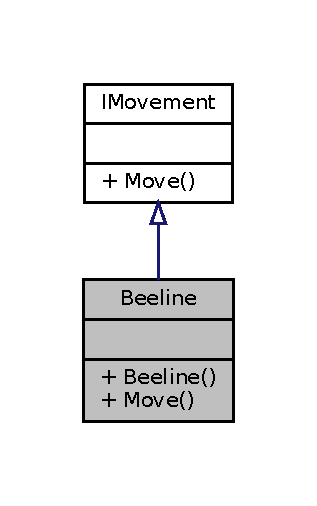
\includegraphics[width=152pt]{classBeeline__inherit__graph}
\end{center}
\end{figure}


Collaboration diagram for Beeline\+:\nopagebreak
\begin{figure}[H]
\begin{center}
\leavevmode
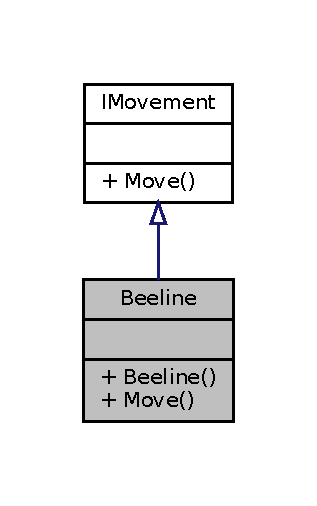
\includegraphics[width=152pt]{classBeeline__coll__graph}
\end{center}
\end{figure}
\subsection*{Public Member Functions}
\begin{DoxyCompactItemize}
\item 
\mbox{\Hypertarget{classBeeline_a352e1d94483d9a3a1e821f1386f23327}\label{classBeeline_a352e1d94483d9a3a1e821f1386f23327}} 
\hyperlink{classBeeline_a352e1d94483d9a3a1e821f1386f23327}{Beeline} ()
\begin{DoxyCompactList}\small\item\em A constructor for an instance of the \hyperlink{classBeeline}{Beeline} class. \end{DoxyCompactList}\item 
void \hyperlink{classBeeline_a1af3f739bafa5a305e39f3b7f278b79d}{Move} (const \hyperlink{classVector3}{Vector3} \&position, std\+::queue$<$ \hyperlink{classVector3}{Vector3} $>$ \&q)
\begin{DoxyCompactList}\small\item\em A method that adds locations to the queue of \hyperlink{classVector3}{Vector3} locations to be visited. \end{DoxyCompactList}\end{DoxyCompactItemize}


\subsection{Detailed Description}
A class that enables a \hyperlink{classBeeline}{Beeline} movement strategy. 

\subsection{Member Function Documentation}
\mbox{\Hypertarget{classBeeline_a1af3f739bafa5a305e39f3b7f278b79d}\label{classBeeline_a1af3f739bafa5a305e39f3b7f278b79d}} 
\index{Beeline@{Beeline}!Move@{Move}}
\index{Move@{Move}!Beeline@{Beeline}}
\subsubsection{\texorpdfstring{Move()}{Move()}}
{\footnotesize\ttfamily void Beeline\+::\+Move (\begin{DoxyParamCaption}\item[{const \hyperlink{classVector3}{Vector3} \&}]{position,  }\item[{std\+::queue$<$ \hyperlink{classVector3}{Vector3} $>$ \&}]{q }\end{DoxyParamCaption})\hspace{0.3cm}{\ttfamily [virtual]}}



A method that adds locations to the queue of \hyperlink{classVector3}{Vector3} locations to be visited. 


\begin{DoxyParams}[1]{Parameters}
\mbox{\tt in}  & {\em position} & A constant reference to a \hyperlink{classVector3}{Vector3} of any location in space. \\
\hline
\mbox{\tt in}  & {\em q} & A reference to a queue of \hyperlink{classVector3}{Vector3} objects that represent the locations to be visited in space. \\
\hline
\end{DoxyParams}


Implements \hyperlink{classIMovement_abe373c52df6be3a5139ab785b13e8964}{I\+Movement}.



The documentation for this class was generated from the following files\+:\begin{DoxyCompactItemize}
\item 
/home/user/repo/project/src/\+Movement/\hyperlink{Beeline_8h}{Beeline.\+h}\item 
/home/user/repo/project/src/\+Movement/\hyperlink{Beeline_8cc}{Beeline.\+cc}\end{DoxyCompactItemize}

\hypertarget{classCamera}{}\section{Camera Class Reference}
\label{classCamera}\index{Camera@{Camera}}


A class that processes and takes picture of what the entity is looking at.  




{\ttfamily \#include $<$Camera.\+h$>$}



Inheritance diagram for Camera\+:\nopagebreak
\begin{figure}[H]
\begin{center}
\leavevmode
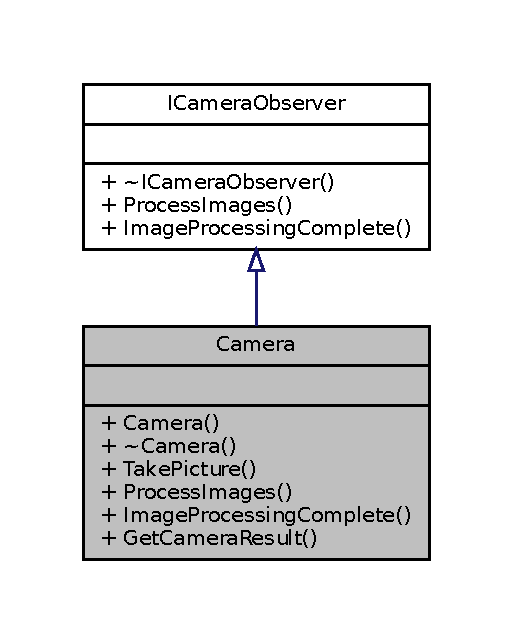
\includegraphics[width=246pt]{classCamera__inherit__graph}
\end{center}
\end{figure}


Collaboration diagram for Camera\+:\nopagebreak
\begin{figure}[H]
\begin{center}
\leavevmode
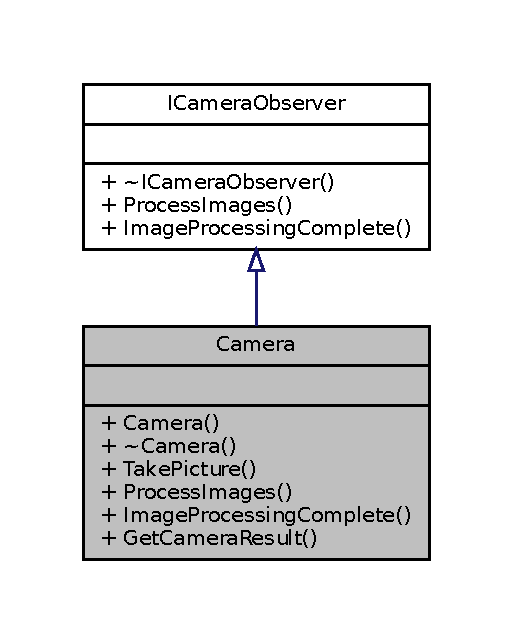
\includegraphics[width=246pt]{classCamera__coll__graph}
\end{center}
\end{figure}
\subsection*{Public Member Functions}
\begin{DoxyCompactItemize}
\item 
\mbox{\Hypertarget{classCamera_aaf2867de230aff68de7d10deae302e8d}\label{classCamera_aaf2867de230aff68de7d10deae302e8d}} 
\hyperlink{classCamera_aaf2867de230aff68de7d10deae302e8d}{Camera} (int id, \hyperlink{classICameraController}{I\+Camera\+Controller} $\ast$controller)
\begin{DoxyCompactList}\small\item\em A constructor for an instance of the \hyperlink{classCamera}{Camera} class. \end{DoxyCompactList}\item 
\mbox{\Hypertarget{classCamera_ad1897942d0ccf91052386388a497349f}\label{classCamera_ad1897942d0ccf91052386388a497349f}} 
\hyperlink{classCamera_ad1897942d0ccf91052386388a497349f}{$\sim$\+Camera} ()
\begin{DoxyCompactList}\small\item\em A destructor (deallocate result mememory). \end{DoxyCompactList}\item 
\mbox{\Hypertarget{classCamera_a70dfc7f06d6e12855afadd358831cf3a}\label{classCamera_a70dfc7f06d6e12855afadd358831cf3a}} 
void \hyperlink{classCamera_a70dfc7f06d6e12855afadd358831cf3a}{Take\+Picture} ()
\begin{DoxyCompactList}\small\item\em Makes the camera take a picture using the specified camera id. \end{DoxyCompactList}\item 
\hyperlink{classICameraResult}{I\+Camera\+Result} $\ast$ \hyperlink{classCamera_a792611ad34a1c595b61b7c72ce1d5e32}{Process\+Images} (int camera\+Id, double x\+Pos, double y\+Pos, double z\+Pos, const std\+::vector$<$ \hyperlink{structRawCameraImage}{Raw\+Camera\+Image} $>$ \&images, picojson\+::object \&details) const
\begin{DoxyCompactList}\small\item\em Processes images asynchronously. The returned camera result will be passed into the Image\+Processing\+Complete(...) method. \end{DoxyCompactList}\item 
void \hyperlink{classCamera_aa44e2101b2cf0a75ab1fd498f3f7adea}{Image\+Processing\+Complete} (\hyperlink{classICameraResult}{I\+Camera\+Result} $\ast$result2)
\begin{DoxyCompactList}\small\item\em After the asynchronous image processing, this method will be synchronized with the update loop. \end{DoxyCompactList}\item 
\hyperlink{classCameraResult}{Camera\+Result} $\ast$ \hyperlink{classCamera_af98a21b496a5d63ca5cc6c813d3c6587}{Get\+Camera\+Result} ()
\begin{DoxyCompactList}\small\item\em Getter for the result of the camera. \end{DoxyCompactList}\end{DoxyCompactItemize}


\subsection{Detailed Description}
A class that processes and takes picture of what the entity is looking at. 

\subsection{Member Function Documentation}
\mbox{\Hypertarget{classCamera_af98a21b496a5d63ca5cc6c813d3c6587}\label{classCamera_af98a21b496a5d63ca5cc6c813d3c6587}} 
\index{Camera@{Camera}!Get\+Camera\+Result@{Get\+Camera\+Result}}
\index{Get\+Camera\+Result@{Get\+Camera\+Result}!Camera@{Camera}}
\subsubsection{\texorpdfstring{Get\+Camera\+Result()}{GetCameraResult()}}
{\footnotesize\ttfamily \hyperlink{classCameraResult}{Camera\+Result} $\ast$ Camera\+::\+Get\+Camera\+Result (\begin{DoxyParamCaption}{ }\end{DoxyParamCaption})}



Getter for the result of the camera. 

\begin{DoxyReturn}{Returns}
\hyperlink{classCamera}{Camera} has a private variable containing the result of the process img that can be shared with the \hyperlink{classEntity}{Entity} owner of the camera through this method 
\end{DoxyReturn}
\mbox{\Hypertarget{classCamera_aa44e2101b2cf0a75ab1fd498f3f7adea}\label{classCamera_aa44e2101b2cf0a75ab1fd498f3f7adea}} 
\index{Camera@{Camera}!Image\+Processing\+Complete@{Image\+Processing\+Complete}}
\index{Image\+Processing\+Complete@{Image\+Processing\+Complete}!Camera@{Camera}}
\subsubsection{\texorpdfstring{Image\+Processing\+Complete()}{ImageProcessingComplete()}}
{\footnotesize\ttfamily void Camera\+::\+Image\+Processing\+Complete (\begin{DoxyParamCaption}\item[{\hyperlink{classICameraResult}{I\+Camera\+Result} $\ast$}]{result2 }\end{DoxyParamCaption})\hspace{0.3cm}{\ttfamily [virtual]}}



After the asynchronous image processing, this method will be synchronized with the update loop. 


\begin{DoxyParams}[1]{Parameters}
\mbox{\tt in}  & {\em result2} & a camera result object if the robot was found with the the position of the robot or a null\+Ptr if robot not found \\
\hline
\end{DoxyParams}


Implements \hyperlink{classICameraObserver_a7d261bd08d570d05032e61b2d5252c88}{I\+Camera\+Observer}.

\mbox{\Hypertarget{classCamera_a792611ad34a1c595b61b7c72ce1d5e32}\label{classCamera_a792611ad34a1c595b61b7c72ce1d5e32}} 
\index{Camera@{Camera}!Process\+Images@{Process\+Images}}
\index{Process\+Images@{Process\+Images}!Camera@{Camera}}
\subsubsection{\texorpdfstring{Process\+Images()}{ProcessImages()}}
{\footnotesize\ttfamily \hyperlink{classICameraResult}{I\+Camera\+Result} $\ast$ Camera\+::\+Process\+Images (\begin{DoxyParamCaption}\item[{int}]{camera\+Id,  }\item[{double}]{x\+Pos,  }\item[{double}]{y\+Pos,  }\item[{double}]{z\+Pos,  }\item[{const std\+::vector$<$ \hyperlink{structRawCameraImage}{Raw\+Camera\+Image} $>$ \&}]{images,  }\item[{picojson\+::object \&}]{details }\end{DoxyParamCaption}) const\hspace{0.3cm}{\ttfamily [virtual]}}



Processes images asynchronously. The returned camera result will be passed into the Image\+Processing\+Complete(...) method. 


\begin{DoxyParams}[1]{Parameters}
\mbox{\tt in}  & {\em camera\+Id} & the id of the camera when created \\
\hline
\mbox{\tt in}  & {\em x\+Pos} & the x position of the camera within the visualization \\
\hline
\mbox{\tt in}  & {\em y\+Pos} & the y position of the camera within the visualization \\
\hline
\mbox{\tt in}  & {\em z\+Pos} & the z position of the camera within the visualization \\
\hline
\mbox{\tt in}  & {\em images} & a vector containing the depth and color img to be process \\
\hline
\mbox{\tt in}  & {\em details} & a picson obj containing extra details\\
\hline
\end{DoxyParams}
\begin{DoxyReturn}{Returns}
a camera result object if the robot was found with the the position of the robot or a null\+Ptr if robot not found 
\end{DoxyReturn}


Implements \hyperlink{classICameraObserver_aec871459f2c429b4334769021b72ec34}{I\+Camera\+Observer}.



The documentation for this class was generated from the following files\+:\begin{DoxyCompactItemize}
\item 
/home/user/repo/project/src/\+Camera/\hyperlink{Camera_8h}{Camera.\+h}\item 
/home/user/repo/project/src/\+Camera/\hyperlink{Camera_8cc}{Camera.\+cc}\end{DoxyCompactItemize}

\hypertarget{classCameraResult}{}\section{Camera\+Result Class Reference}
\label{classCameraResult}\index{Camera\+Result@{Camera\+Result}}


A class that strores the result of processing an img when looking for a robot.  




{\ttfamily \#include $<$Camera\+Result.\+h$>$}



Inheritance diagram for Camera\+Result\+:\nopagebreak
\begin{figure}[H]
\begin{center}
\leavevmode
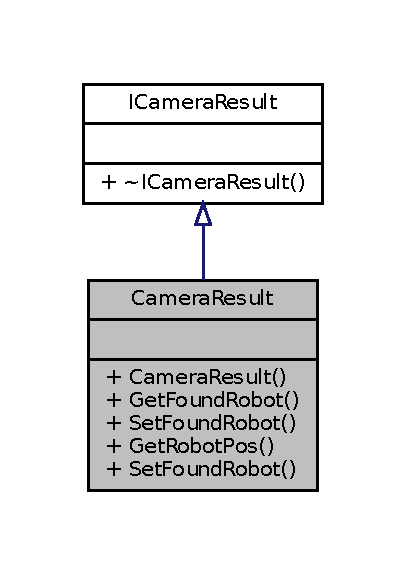
\includegraphics[width=195pt]{classCameraResult__inherit__graph}
\end{center}
\end{figure}


Collaboration diagram for Camera\+Result\+:\nopagebreak
\begin{figure}[H]
\begin{center}
\leavevmode
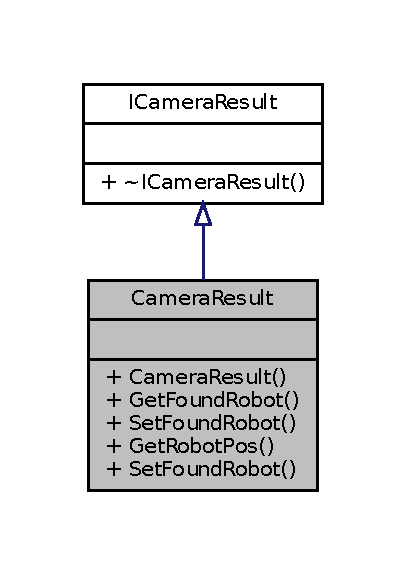
\includegraphics[width=195pt]{classCameraResult__coll__graph}
\end{center}
\end{figure}
\subsection*{Public Member Functions}
\begin{DoxyCompactItemize}
\item 
\mbox{\Hypertarget{classCameraResult_aac91602d9a7322df55bf0e3bf0c32e39}\label{classCameraResult_aac91602d9a7322df55bf0e3bf0c32e39}} 
\hyperlink{classCameraResult_aac91602d9a7322df55bf0e3bf0c32e39}{Camera\+Result} ()
\begin{DoxyCompactList}\small\item\em An empty constructor. \end{DoxyCompactList}\item 
bool \hyperlink{classCameraResult_ab9285652d06715797fee95132a51fbf6}{Get\+Found\+Robot} () const
\begin{DoxyCompactList}\small\item\em Getter of img result. \end{DoxyCompactList}\item 
void \hyperlink{classCameraResult_a764f0b2b6fa57734ebf45703c79e071c}{Set\+Found\+Robot} (bool f)
\begin{DoxyCompactList}\small\item\em Setter of img result. \end{DoxyCompactList}\item 
\hyperlink{classVector3}{Vector3} \hyperlink{classCameraResult_a12314f7a760e9eaa5fd949afc3289d54}{Get\+Robot\+Pos} () const
\begin{DoxyCompactList}\small\item\em Getter of robot position. \end{DoxyCompactList}\item 
void \hyperlink{classCameraResult_a669e85149ff4bf617c136afa57577bbf}{Set\+Found\+Robot} (\hyperlink{classVector3}{Vector3} pos)
\begin{DoxyCompactList}\small\item\em Setter of robot pos. \end{DoxyCompactList}\end{DoxyCompactItemize}


\subsection{Detailed Description}
A class that strores the result of processing an img when looking for a robot. 

\subsection{Member Function Documentation}
\mbox{\Hypertarget{classCameraResult_ab9285652d06715797fee95132a51fbf6}\label{classCameraResult_ab9285652d06715797fee95132a51fbf6}} 
\index{Camera\+Result@{Camera\+Result}!Get\+Found\+Robot@{Get\+Found\+Robot}}
\index{Get\+Found\+Robot@{Get\+Found\+Robot}!Camera\+Result@{Camera\+Result}}
\subsubsection{\texorpdfstring{Get\+Found\+Robot()}{GetFoundRobot()}}
{\footnotesize\ttfamily bool Camera\+Result\+::\+Get\+Found\+Robot (\begin{DoxyParamCaption}{ }\end{DoxyParamCaption}) const}



Getter of img result. 

\begin{DoxyReturn}{Returns}
true if robot was found when processing this img, false otherwise 
\end{DoxyReturn}
\mbox{\Hypertarget{classCameraResult_a12314f7a760e9eaa5fd949afc3289d54}\label{classCameraResult_a12314f7a760e9eaa5fd949afc3289d54}} 
\index{Camera\+Result@{Camera\+Result}!Get\+Robot\+Pos@{Get\+Robot\+Pos}}
\index{Get\+Robot\+Pos@{Get\+Robot\+Pos}!Camera\+Result@{Camera\+Result}}
\subsubsection{\texorpdfstring{Get\+Robot\+Pos()}{GetRobotPos()}}
{\footnotesize\ttfamily \hyperlink{classVector3}{Vector3} Camera\+Result\+::\+Get\+Robot\+Pos (\begin{DoxyParamCaption}{ }\end{DoxyParamCaption}) const}



Getter of robot position. 

\begin{DoxyReturn}{Returns}
a \hyperlink{classVector3}{Vector3} with the x,y,z values of where the robot is located in the map 
\end{DoxyReturn}
\mbox{\Hypertarget{classCameraResult_a764f0b2b6fa57734ebf45703c79e071c}\label{classCameraResult_a764f0b2b6fa57734ebf45703c79e071c}} 
\index{Camera\+Result@{Camera\+Result}!Set\+Found\+Robot@{Set\+Found\+Robot}}
\index{Set\+Found\+Robot@{Set\+Found\+Robot}!Camera\+Result@{Camera\+Result}}
\subsubsection{\texorpdfstring{Set\+Found\+Robot()}{SetFoundRobot()}\hspace{0.1cm}{\footnotesize\ttfamily [1/2]}}
{\footnotesize\ttfamily void Camera\+Result\+::\+Set\+Found\+Robot (\begin{DoxyParamCaption}\item[{bool}]{f }\end{DoxyParamCaption})}



Setter of img result. 


\begin{DoxyParams}[1]{Parameters}
\mbox{\tt in}  & {\em f} & true if robot was found when processing this img, false otherwise \\
\hline
\end{DoxyParams}
\mbox{\Hypertarget{classCameraResult_a669e85149ff4bf617c136afa57577bbf}\label{classCameraResult_a669e85149ff4bf617c136afa57577bbf}} 
\index{Camera\+Result@{Camera\+Result}!Set\+Found\+Robot@{Set\+Found\+Robot}}
\index{Set\+Found\+Robot@{Set\+Found\+Robot}!Camera\+Result@{Camera\+Result}}
\subsubsection{\texorpdfstring{Set\+Found\+Robot()}{SetFoundRobot()}\hspace{0.1cm}{\footnotesize\ttfamily [2/2]}}
{\footnotesize\ttfamily void Camera\+Result\+::\+Set\+Found\+Robot (\begin{DoxyParamCaption}\item[{\hyperlink{classVector3}{Vector3}}]{pos }\end{DoxyParamCaption})}



Setter of robot pos. 


\begin{DoxyParams}[1]{Parameters}
\mbox{\tt in}  & {\em pos} & a \hyperlink{classVector3}{Vector3} with the x,y,z values of where the robot is located in the map \\
\hline
\end{DoxyParams}


The documentation for this class was generated from the following files\+:\begin{DoxyCompactItemize}
\item 
/home/user/repo/project/src/\+Camera/\hyperlink{CameraResult_8h}{Camera\+Result.\+h}\item 
/home/user/repo/project/src/\+Camera/\hyperlink{CameraResult_8cc}{Camera\+Result.\+cc}\end{DoxyCompactItemize}

\hypertarget{classCanny}{}\section{Canny Class Reference}
\label{classCanny}\index{Canny@{Canny}}


A filter that applies the greyscale, gaussian, sobel, non-\/max suppression, double threshold, and hysteresis filters to an \hyperlink{classImage}{Image}.  




{\ttfamily \#include $<$canny.\+h$>$}



Inheritance diagram for Canny\+:\nopagebreak
\begin{figure}[H]
\begin{center}
\leavevmode
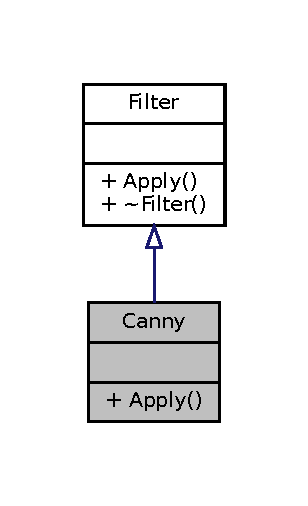
\includegraphics[width=148pt]{classCanny__inherit__graph}
\end{center}
\end{figure}


Collaboration diagram for Canny\+:\nopagebreak
\begin{figure}[H]
\begin{center}
\leavevmode
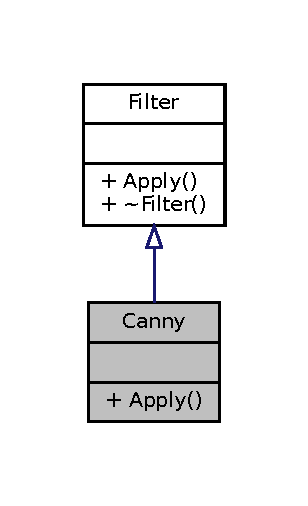
\includegraphics[width=148pt]{classCanny__coll__graph}
\end{center}
\end{figure}
\subsection*{Public Member Functions}
\begin{DoxyCompactItemize}
\item 
void \hyperlink{classCanny_aefadd0d0166f26f76d6bf2cf59dae3aa}{Apply} (std\+::vector$<$ \hyperlink{classImage}{Image} $\ast$$>$ original, std\+::vector$<$ \hyperlink{classImage}{Image} $\ast$$>$ filtered)
\begin{DoxyCompactList}\small\item\em method that applies all the filters required for canny edge detection \end{DoxyCompactList}\end{DoxyCompactItemize}


\subsection{Detailed Description}
A filter that applies the greyscale, gaussian, sobel, non-\/max suppression, double threshold, and hysteresis filters to an \hyperlink{classImage}{Image}. 

\subsection{Member Function Documentation}
\mbox{\Hypertarget{classCanny_aefadd0d0166f26f76d6bf2cf59dae3aa}\label{classCanny_aefadd0d0166f26f76d6bf2cf59dae3aa}} 
\index{Canny@{Canny}!Apply@{Apply}}
\index{Apply@{Apply}!Canny@{Canny}}
\subsubsection{\texorpdfstring{Apply()}{Apply()}}
{\footnotesize\ttfamily void Canny\+::\+Apply (\begin{DoxyParamCaption}\item[{std\+::vector$<$ \hyperlink{classImage}{Image} $\ast$$>$}]{original,  }\item[{std\+::vector$<$ \hyperlink{classImage}{Image} $\ast$$>$}]{filtered }\end{DoxyParamCaption})\hspace{0.3cm}{\ttfamily [virtual]}}



method that applies all the filters required for canny edge detection 


\begin{DoxyParams}{Parameters}
{\em original} & A vector of input images to apply the filter over. \\
\hline
{\em filtered} & A vector of output images that displays the original images filtered. \\
\hline
\end{DoxyParams}


Implements \hyperlink{classFilter_afab0d50af44a19a370ebe46c69b8ff4e}{Filter}.



The documentation for this class was generated from the following files\+:\begin{DoxyCompactItemize}
\item 
/home/user/repo/project/\+Image\+Processing/\hyperlink{canny_8h}{canny.\+h}\item 
/home/user/repo/project/\+Image\+Processing/\hyperlink{canny_8cc}{canny.\+cc}\end{DoxyCompactItemize}

\hypertarget{classColor}{}\section{Color Class Reference}
\label{classColor}\index{Color@{Color}}


A class that represents a pixel. Each component of the color is represented by a value between 0 and 255.  




{\ttfamily \#include $<$color.\+h$>$}



Collaboration diagram for Color\+:\nopagebreak
\begin{figure}[H]
\begin{center}
\leavevmode
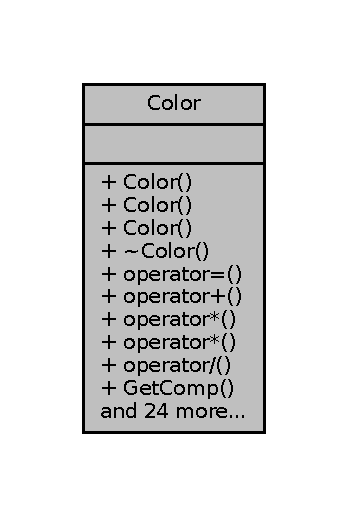
\includegraphics[width=167pt]{classColor__coll__graph}
\end{center}
\end{figure}
\subsection*{Public Member Functions}
\begin{DoxyCompactItemize}
\item 
\mbox{\Hypertarget{classColor_a9a742cbe9f9f4037f5d9f4e81a9b2428}\label{classColor_a9a742cbe9f9f4037f5d9f4e81a9b2428}} 
\hyperlink{classColor_a9a742cbe9f9f4037f5d9f4e81a9b2428}{Color} ()
\begin{DoxyCompactList}\small\item\em Default constructor accepting no parameters. \end{DoxyCompactList}\item 
\hyperlink{classColor_a18c0e82aae9dfe069aea5d2326ee4b4b}{Color} (std\+::unique\+\_\+ptr$<$ float\mbox{[}$\,$\mbox{]}$>$ \&pixel, int num\+Of\+Components)
\begin{DoxyCompactList}\small\item\em Constructor that accepts color component values. \end{DoxyCompactList}\item 
\hyperlink{classColor_a7b075d27e3bbdde7cbe648dc3b804261}{Color} (const \hyperlink{classColor}{Color} \&color)
\begin{DoxyCompactList}\small\item\em A copy constructor that allows to copy/duplicate any \hyperlink{classColor}{Color}. \end{DoxyCompactList}\item 
\mbox{\Hypertarget{classColor_a3cfce6c6821d3bf489e26074c55378c0}\label{classColor_a3cfce6c6821d3bf489e26074c55378c0}} 
\hyperlink{classColor_a3cfce6c6821d3bf489e26074c55378c0}{$\sim$\+Color} ()
\begin{DoxyCompactList}\small\item\em A destructor. \end{DoxyCompactList}\item 
void \hyperlink{classColor_ac06dcf409ae64de5a67c7f6e69b6f44b}{operator=} (const \hyperlink{classColor}{Color} \&color)
\begin{DoxyCompactList}\small\item\em Performs a deep copy of the color object passed in. \end{DoxyCompactList}\item 
\hyperlink{classColor}{Color} \hyperlink{classColor_acd40b26ca2f9217b5cde1e5c1251ef04}{operator+} (const \hyperlink{classColor}{Color} \&color) const
\begin{DoxyCompactList}\small\item\em Performs the component-\/wise sum of two colors. Components that exceed 255 are N\+OT truncated to 255. \end{DoxyCompactList}\item 
\hyperlink{classColor}{Color} \hyperlink{classColor_a6cc052b0ca852fb8703e642e49fcdbe9}{operator$\ast$} (const \hyperlink{classColor}{Color} \&color) const
\begin{DoxyCompactList}\small\item\em Performs the component-\/wise multiplication of two colors. Components that exceed 255 are N\+OT truncated to 255. \end{DoxyCompactList}\item 
\hyperlink{classColor}{Color} \hyperlink{classColor_a1913ac35b2deeabf7f9bc449deae499e}{operator$\ast$} (float factor) const
\begin{DoxyCompactList}\small\item\em Performs the component-\/wise multiplication of a color and a float, it multiplies each component of the color by the float passed as parameter. Components that exceed 255 are N\+OT truncated to 255. \end{DoxyCompactList}\item 
\hyperlink{classColor}{Color} \hyperlink{classColor_ac1591338c7f8714e3683cca15ffb2fd3}{operator/} (float factor) const
\begin{DoxyCompactList}\small\item\em Performs the component-\/wise division of a color and a float, it divides each component of the color by the float passed as parameter. \end{DoxyCompactList}\item 
int \hyperlink{classColor_ae63e798d250d1b1393008e019a054253}{Get\+Comp} () const
\item 
float \hyperlink{classColor_aaf750ff9360c9eb6abf1de07ec710c1e}{Get\+Red} () const
\item 
float \hyperlink{classColor_a0c1d09e2435aefad98931d765bc36d01}{Get\+Green} () const
\item 
float \hyperlink{classColor_a79e225ea938465a072b697b9431f8150}{Get\+Blue} () const
\item 
float \hyperlink{classColor_a1eb5d3ba0276e2b555211aae3cd500b6}{Get\+Alpha} () const
\item 
\mbox{\Hypertarget{classColor_afcdaa6ae749a1325edc313429a3a87d3}\label{classColor_afcdaa6ae749a1325edc313429a3a87d3}} 
void \hyperlink{classColor_afcdaa6ae749a1325edc313429a3a87d3}{Set\+Alpha} (float val)
\begin{DoxyCompactList}\small\item\em Sets the alpha component to the new float value passed in as the val parameter. \end{DoxyCompactList}\item 
float \hyperlink{classColor_ae8aa52d3ec0bb13f4f9732d9487a5431}{Get\+Val} (int component) const
\item 
float \hyperlink{classColor_a196417267fdde68255f53164c5eff701}{Get\+Luminance} () const
\begin{DoxyCompactList}\small\item\em Calculates the brightness of the color according to a weighted sum of the R\+GB components of the color. \end{DoxyCompactList}\item 
\mbox{\Hypertarget{classColor_a9a742cbe9f9f4037f5d9f4e81a9b2428}\label{classColor_a9a742cbe9f9f4037f5d9f4e81a9b2428}} 
\hyperlink{classColor_a9a742cbe9f9f4037f5d9f4e81a9b2428}{Color} ()
\begin{DoxyCompactList}\small\item\em Default constructor accepting no parameters. \end{DoxyCompactList}\item 
\hyperlink{classColor_a18c0e82aae9dfe069aea5d2326ee4b4b}{Color} (std\+::unique\+\_\+ptr$<$ float\mbox{[}$\,$\mbox{]}$>$ \&pixel, int num\+Of\+Components)
\begin{DoxyCompactList}\small\item\em Constructor that accepts color component values. \end{DoxyCompactList}\item 
\hyperlink{classColor_a7b075d27e3bbdde7cbe648dc3b804261}{Color} (const \hyperlink{classColor}{Color} \&color)
\begin{DoxyCompactList}\small\item\em A copy constructor that allows to copy/duplicate any \hyperlink{classColor}{Color}. \end{DoxyCompactList}\item 
\mbox{\Hypertarget{classColor_a3cfce6c6821d3bf489e26074c55378c0}\label{classColor_a3cfce6c6821d3bf489e26074c55378c0}} 
\hyperlink{classColor_a3cfce6c6821d3bf489e26074c55378c0}{$\sim$\+Color} ()
\begin{DoxyCompactList}\small\item\em A destructor. \end{DoxyCompactList}\item 
void \hyperlink{classColor_ac06dcf409ae64de5a67c7f6e69b6f44b}{operator=} (const \hyperlink{classColor}{Color} \&color)
\begin{DoxyCompactList}\small\item\em Performs a deep copy of the color object passed in. \end{DoxyCompactList}\item 
\hyperlink{classColor}{Color} \hyperlink{classColor_acd40b26ca2f9217b5cde1e5c1251ef04}{operator+} (const \hyperlink{classColor}{Color} \&color) const
\begin{DoxyCompactList}\small\item\em Performs the component-\/wise sum of two colors. Components that exceed 255 are N\+OT truncated to 255. \end{DoxyCompactList}\item 
\hyperlink{classColor}{Color} \hyperlink{classColor_a6cc052b0ca852fb8703e642e49fcdbe9}{operator$\ast$} (const \hyperlink{classColor}{Color} \&color) const
\begin{DoxyCompactList}\small\item\em Performs the component-\/wise multiplication of two colors. Components that exceed 255 are N\+OT truncated to 255. \end{DoxyCompactList}\item 
\hyperlink{classColor}{Color} \hyperlink{classColor_a1913ac35b2deeabf7f9bc449deae499e}{operator$\ast$} (float factor) const
\begin{DoxyCompactList}\small\item\em Performs the component-\/wise multiplication of a color and a float, it multiplies each component of the color by the float passed as parameter. Components that exceed 255 are N\+OT truncated to 255. \end{DoxyCompactList}\item 
\hyperlink{classColor}{Color} \hyperlink{classColor_ac1591338c7f8714e3683cca15ffb2fd3}{operator/} (float factor) const
\begin{DoxyCompactList}\small\item\em Performs the component-\/wise division of a color and a float, it divides each component of the color by the float passed as parameter. \end{DoxyCompactList}\item 
int \hyperlink{classColor_ae63e798d250d1b1393008e019a054253}{Get\+Comp} () const
\item 
float \hyperlink{classColor_aaf750ff9360c9eb6abf1de07ec710c1e}{Get\+Red} () const
\item 
float \hyperlink{classColor_a0c1d09e2435aefad98931d765bc36d01}{Get\+Green} () const
\item 
float \hyperlink{classColor_a79e225ea938465a072b697b9431f8150}{Get\+Blue} () const
\item 
float \hyperlink{classColor_a1eb5d3ba0276e2b555211aae3cd500b6}{Get\+Alpha} () const
\item 
\mbox{\Hypertarget{classColor_afcdaa6ae749a1325edc313429a3a87d3}\label{classColor_afcdaa6ae749a1325edc313429a3a87d3}} 
void \hyperlink{classColor_afcdaa6ae749a1325edc313429a3a87d3}{Set\+Alpha} (float val)
\begin{DoxyCompactList}\small\item\em Sets the alpha component to the new float value passed in as the val parameter. \end{DoxyCompactList}\item 
float \hyperlink{classColor_ae8aa52d3ec0bb13f4f9732d9487a5431}{Get\+Val} (int component) const
\item 
float \hyperlink{classColor_a196417267fdde68255f53164c5eff701}{Get\+Luminance} () const
\begin{DoxyCompactList}\small\item\em Calculates the brightness of the color according to a weighted sum of the R\+GB components of the color. \end{DoxyCompactList}\end{DoxyCompactItemize}


\subsection{Detailed Description}
A class that represents a pixel. Each component of the color is represented by a value between 0 and 255. 

\subsection{Constructor \& Destructor Documentation}
\mbox{\Hypertarget{classColor_a18c0e82aae9dfe069aea5d2326ee4b4b}\label{classColor_a18c0e82aae9dfe069aea5d2326ee4b4b}} 
\index{Color@{Color}!Color@{Color}}
\index{Color@{Color}!Color@{Color}}
\subsubsection{\texorpdfstring{Color()}{Color()}\hspace{0.1cm}{\footnotesize\ttfamily [1/4]}}
{\footnotesize\ttfamily Color\+::\+Color (\begin{DoxyParamCaption}\item[{std\+::unique\+\_\+ptr$<$ float\mbox{[}$\,$\mbox{]}$>$ \&}]{pixel,  }\item[{int}]{num\+Of\+Components }\end{DoxyParamCaption})}



Constructor that accepts color component values. 


\begin{DoxyParams}[1]{Parameters}
\mbox{\tt in}  & {\em pixel} & A unique pointer float array containing all the color coponents, such as rgba values of the pixel. \\
\hline
\mbox{\tt in}  & {\em num\+Of\+Components} & The number of components the \hyperlink{classColor}{Color} object has, which is the length of the pixel unique pointer float array. \\
\hline
\end{DoxyParams}
\mbox{\Hypertarget{classColor_a7b075d27e3bbdde7cbe648dc3b804261}\label{classColor_a7b075d27e3bbdde7cbe648dc3b804261}} 
\index{Color@{Color}!Color@{Color}}
\index{Color@{Color}!Color@{Color}}
\subsubsection{\texorpdfstring{Color()}{Color()}\hspace{0.1cm}{\footnotesize\ttfamily [2/4]}}
{\footnotesize\ttfamily Color\+::\+Color (\begin{DoxyParamCaption}\item[{const \hyperlink{classColor}{Color} \&}]{color }\end{DoxyParamCaption})}



A copy constructor that allows to copy/duplicate any \hyperlink{classColor}{Color}. 


\begin{DoxyParams}[1]{Parameters}
\mbox{\tt in}  & {\em color} & The \hyperlink{classColor}{Color} object to make a deep copy from. \\
\hline
\end{DoxyParams}
\mbox{\Hypertarget{classColor_a18c0e82aae9dfe069aea5d2326ee4b4b}\label{classColor_a18c0e82aae9dfe069aea5d2326ee4b4b}} 
\index{Color@{Color}!Color@{Color}}
\index{Color@{Color}!Color@{Color}}
\subsubsection{\texorpdfstring{Color()}{Color()}\hspace{0.1cm}{\footnotesize\ttfamily [3/4]}}
{\footnotesize\ttfamily Color\+::\+Color (\begin{DoxyParamCaption}\item[{std\+::unique\+\_\+ptr$<$ float\mbox{[}$\,$\mbox{]}$>$ \&}]{pixel,  }\item[{int}]{num\+Of\+Components }\end{DoxyParamCaption})}



Constructor that accepts color component values. 


\begin{DoxyParams}[1]{Parameters}
\mbox{\tt in}  & {\em pixel} & A unique pointer float array containing all the color coponents, such as rgba values of the pixel. \\
\hline
\mbox{\tt in}  & {\em num\+Of\+Components} & The number of components the \hyperlink{classColor}{Color} object has, which is the length of the pixel unique pointer float array. \\
\hline
\end{DoxyParams}
\mbox{\Hypertarget{classColor_a7b075d27e3bbdde7cbe648dc3b804261}\label{classColor_a7b075d27e3bbdde7cbe648dc3b804261}} 
\index{Color@{Color}!Color@{Color}}
\index{Color@{Color}!Color@{Color}}
\subsubsection{\texorpdfstring{Color()}{Color()}\hspace{0.1cm}{\footnotesize\ttfamily [4/4]}}
{\footnotesize\ttfamily Color\+::\+Color (\begin{DoxyParamCaption}\item[{const \hyperlink{classColor}{Color} \&}]{color }\end{DoxyParamCaption})}



A copy constructor that allows to copy/duplicate any \hyperlink{classColor}{Color}. 


\begin{DoxyParams}[1]{Parameters}
\mbox{\tt in}  & {\em color} & The \hyperlink{classColor}{Color} object to make a deep copy from. \\
\hline
\end{DoxyParams}


\subsection{Member Function Documentation}
\mbox{\Hypertarget{classColor_a1eb5d3ba0276e2b555211aae3cd500b6}\label{classColor_a1eb5d3ba0276e2b555211aae3cd500b6}} 
\index{Color@{Color}!Get\+Alpha@{Get\+Alpha}}
\index{Get\+Alpha@{Get\+Alpha}!Color@{Color}}
\subsubsection{\texorpdfstring{Get\+Alpha()}{GetAlpha()}\hspace{0.1cm}{\footnotesize\ttfamily [1/2]}}
{\footnotesize\ttfamily float Color\+::\+Get\+Alpha (\begin{DoxyParamCaption}{ }\end{DoxyParamCaption}) const\hspace{0.3cm}{\ttfamily [inline]}}

\begin{DoxyReturn}{Returns}
The alpha value component of the color. 
\end{DoxyReturn}
\mbox{\Hypertarget{classColor_a1eb5d3ba0276e2b555211aae3cd500b6}\label{classColor_a1eb5d3ba0276e2b555211aae3cd500b6}} 
\index{Color@{Color}!Get\+Alpha@{Get\+Alpha}}
\index{Get\+Alpha@{Get\+Alpha}!Color@{Color}}
\subsubsection{\texorpdfstring{Get\+Alpha()}{GetAlpha()}\hspace{0.1cm}{\footnotesize\ttfamily [2/2]}}
{\footnotesize\ttfamily float Color\+::\+Get\+Alpha (\begin{DoxyParamCaption}{ }\end{DoxyParamCaption}) const\hspace{0.3cm}{\ttfamily [inline]}}

\begin{DoxyReturn}{Returns}
The alpha value component of the color. 
\end{DoxyReturn}
\mbox{\Hypertarget{classColor_a79e225ea938465a072b697b9431f8150}\label{classColor_a79e225ea938465a072b697b9431f8150}} 
\index{Color@{Color}!Get\+Blue@{Get\+Blue}}
\index{Get\+Blue@{Get\+Blue}!Color@{Color}}
\subsubsection{\texorpdfstring{Get\+Blue()}{GetBlue()}\hspace{0.1cm}{\footnotesize\ttfamily [1/2]}}
{\footnotesize\ttfamily float Color\+::\+Get\+Blue (\begin{DoxyParamCaption}{ }\end{DoxyParamCaption}) const\hspace{0.3cm}{\ttfamily [inline]}}

\begin{DoxyReturn}{Returns}
The blue value component of the color. 
\end{DoxyReturn}
\mbox{\Hypertarget{classColor_a79e225ea938465a072b697b9431f8150}\label{classColor_a79e225ea938465a072b697b9431f8150}} 
\index{Color@{Color}!Get\+Blue@{Get\+Blue}}
\index{Get\+Blue@{Get\+Blue}!Color@{Color}}
\subsubsection{\texorpdfstring{Get\+Blue()}{GetBlue()}\hspace{0.1cm}{\footnotesize\ttfamily [2/2]}}
{\footnotesize\ttfamily float Color\+::\+Get\+Blue (\begin{DoxyParamCaption}{ }\end{DoxyParamCaption}) const\hspace{0.3cm}{\ttfamily [inline]}}

\begin{DoxyReturn}{Returns}
The blue value component of the color. 
\end{DoxyReturn}
\mbox{\Hypertarget{classColor_ae63e798d250d1b1393008e019a054253}\label{classColor_ae63e798d250d1b1393008e019a054253}} 
\index{Color@{Color}!Get\+Comp@{Get\+Comp}}
\index{Get\+Comp@{Get\+Comp}!Color@{Color}}
\subsubsection{\texorpdfstring{Get\+Comp()}{GetComp()}\hspace{0.1cm}{\footnotesize\ttfamily [1/2]}}
{\footnotesize\ttfamily int Color\+::\+Get\+Comp (\begin{DoxyParamCaption}{ }\end{DoxyParamCaption}) const\hspace{0.3cm}{\ttfamily [inline]}}

\begin{DoxyReturn}{Returns}
The number of components that color object holds. 
\end{DoxyReturn}
\mbox{\Hypertarget{classColor_ae63e798d250d1b1393008e019a054253}\label{classColor_ae63e798d250d1b1393008e019a054253}} 
\index{Color@{Color}!Get\+Comp@{Get\+Comp}}
\index{Get\+Comp@{Get\+Comp}!Color@{Color}}
\subsubsection{\texorpdfstring{Get\+Comp()}{GetComp()}\hspace{0.1cm}{\footnotesize\ttfamily [2/2]}}
{\footnotesize\ttfamily int Color\+::\+Get\+Comp (\begin{DoxyParamCaption}{ }\end{DoxyParamCaption}) const\hspace{0.3cm}{\ttfamily [inline]}}

\begin{DoxyReturn}{Returns}
The number of components that color object holds. 
\end{DoxyReturn}
\mbox{\Hypertarget{classColor_a0c1d09e2435aefad98931d765bc36d01}\label{classColor_a0c1d09e2435aefad98931d765bc36d01}} 
\index{Color@{Color}!Get\+Green@{Get\+Green}}
\index{Get\+Green@{Get\+Green}!Color@{Color}}
\subsubsection{\texorpdfstring{Get\+Green()}{GetGreen()}\hspace{0.1cm}{\footnotesize\ttfamily [1/2]}}
{\footnotesize\ttfamily float Color\+::\+Get\+Green (\begin{DoxyParamCaption}{ }\end{DoxyParamCaption}) const\hspace{0.3cm}{\ttfamily [inline]}}

\begin{DoxyReturn}{Returns}
The green value component of the color. 
\end{DoxyReturn}
\mbox{\Hypertarget{classColor_a0c1d09e2435aefad98931d765bc36d01}\label{classColor_a0c1d09e2435aefad98931d765bc36d01}} 
\index{Color@{Color}!Get\+Green@{Get\+Green}}
\index{Get\+Green@{Get\+Green}!Color@{Color}}
\subsubsection{\texorpdfstring{Get\+Green()}{GetGreen()}\hspace{0.1cm}{\footnotesize\ttfamily [2/2]}}
{\footnotesize\ttfamily float Color\+::\+Get\+Green (\begin{DoxyParamCaption}{ }\end{DoxyParamCaption}) const\hspace{0.3cm}{\ttfamily [inline]}}

\begin{DoxyReturn}{Returns}
The green value component of the color. 
\end{DoxyReturn}
\mbox{\Hypertarget{classColor_a196417267fdde68255f53164c5eff701}\label{classColor_a196417267fdde68255f53164c5eff701}} 
\index{Color@{Color}!Get\+Luminance@{Get\+Luminance}}
\index{Get\+Luminance@{Get\+Luminance}!Color@{Color}}
\subsubsection{\texorpdfstring{Get\+Luminance()}{GetLuminance()}\hspace{0.1cm}{\footnotesize\ttfamily [1/2]}}
{\footnotesize\ttfamily float Color\+::\+Get\+Luminance (\begin{DoxyParamCaption}{ }\end{DoxyParamCaption}) const\hspace{0.3cm}{\ttfamily [inline]}}



Calculates the brightness of the color according to a weighted sum of the R\+GB components of the color. 

\begin{DoxyReturn}{Returns}
A float representing the brightness of the color. 
\end{DoxyReturn}
\mbox{\Hypertarget{classColor_a196417267fdde68255f53164c5eff701}\label{classColor_a196417267fdde68255f53164c5eff701}} 
\index{Color@{Color}!Get\+Luminance@{Get\+Luminance}}
\index{Get\+Luminance@{Get\+Luminance}!Color@{Color}}
\subsubsection{\texorpdfstring{Get\+Luminance()}{GetLuminance()}\hspace{0.1cm}{\footnotesize\ttfamily [2/2]}}
{\footnotesize\ttfamily float Color\+::\+Get\+Luminance (\begin{DoxyParamCaption}{ }\end{DoxyParamCaption}) const\hspace{0.3cm}{\ttfamily [inline]}}



Calculates the brightness of the color according to a weighted sum of the R\+GB components of the color. 

\begin{DoxyReturn}{Returns}
A float representing the brightness of the color. 
\end{DoxyReturn}
\mbox{\Hypertarget{classColor_aaf750ff9360c9eb6abf1de07ec710c1e}\label{classColor_aaf750ff9360c9eb6abf1de07ec710c1e}} 
\index{Color@{Color}!Get\+Red@{Get\+Red}}
\index{Get\+Red@{Get\+Red}!Color@{Color}}
\subsubsection{\texorpdfstring{Get\+Red()}{GetRed()}\hspace{0.1cm}{\footnotesize\ttfamily [1/2]}}
{\footnotesize\ttfamily float Color\+::\+Get\+Red (\begin{DoxyParamCaption}{ }\end{DoxyParamCaption}) const\hspace{0.3cm}{\ttfamily [inline]}}

\begin{DoxyReturn}{Returns}
The red value component of the color. 
\end{DoxyReturn}
\mbox{\Hypertarget{classColor_aaf750ff9360c9eb6abf1de07ec710c1e}\label{classColor_aaf750ff9360c9eb6abf1de07ec710c1e}} 
\index{Color@{Color}!Get\+Red@{Get\+Red}}
\index{Get\+Red@{Get\+Red}!Color@{Color}}
\subsubsection{\texorpdfstring{Get\+Red()}{GetRed()}\hspace{0.1cm}{\footnotesize\ttfamily [2/2]}}
{\footnotesize\ttfamily float Color\+::\+Get\+Red (\begin{DoxyParamCaption}{ }\end{DoxyParamCaption}) const\hspace{0.3cm}{\ttfamily [inline]}}

\begin{DoxyReturn}{Returns}
The red value component of the color. 
\end{DoxyReturn}
\mbox{\Hypertarget{classColor_ae8aa52d3ec0bb13f4f9732d9487a5431}\label{classColor_ae8aa52d3ec0bb13f4f9732d9487a5431}} 
\index{Color@{Color}!Get\+Val@{Get\+Val}}
\index{Get\+Val@{Get\+Val}!Color@{Color}}
\subsubsection{\texorpdfstring{Get\+Val()}{GetVal()}\hspace{0.1cm}{\footnotesize\ttfamily [1/2]}}
{\footnotesize\ttfamily float Color\+::\+Get\+Val (\begin{DoxyParamCaption}\item[{int}]{component }\end{DoxyParamCaption}) const\hspace{0.3cm}{\ttfamily [inline]}}

\begin{DoxyReturn}{Returns}
The value component of the color that is represented by the indexed passed in as the component parameter.
\end{DoxyReturn}

\begin{DoxyParams}[1]{Parameters}
\mbox{\tt in}  & {\em Returns} & the value of the color component of the index that was specified to be retrieved. \\
\hline
\end{DoxyParams}
\mbox{\Hypertarget{classColor_ae8aa52d3ec0bb13f4f9732d9487a5431}\label{classColor_ae8aa52d3ec0bb13f4f9732d9487a5431}} 
\index{Color@{Color}!Get\+Val@{Get\+Val}}
\index{Get\+Val@{Get\+Val}!Color@{Color}}
\subsubsection{\texorpdfstring{Get\+Val()}{GetVal()}\hspace{0.1cm}{\footnotesize\ttfamily [2/2]}}
{\footnotesize\ttfamily float Color\+::\+Get\+Val (\begin{DoxyParamCaption}\item[{int}]{component }\end{DoxyParamCaption}) const\hspace{0.3cm}{\ttfamily [inline]}}

\begin{DoxyReturn}{Returns}
The value component of the color that is represented by the indexed passed in as the component parameter.
\end{DoxyReturn}

\begin{DoxyParams}[1]{Parameters}
\mbox{\tt in}  & {\em Returns} & the value of the color component of the index that was specified to be retrieved. \\
\hline
\end{DoxyParams}
\mbox{\Hypertarget{classColor_a6cc052b0ca852fb8703e642e49fcdbe9}\label{classColor_a6cc052b0ca852fb8703e642e49fcdbe9}} 
\index{Color@{Color}!operator$\ast$@{operator$\ast$}}
\index{operator$\ast$@{operator$\ast$}!Color@{Color}}
\subsubsection{\texorpdfstring{operator$\ast$()}{operator*()}\hspace{0.1cm}{\footnotesize\ttfamily [1/4]}}
{\footnotesize\ttfamily \hyperlink{classColor}{Color} Color\+::operator$\ast$ (\begin{DoxyParamCaption}\item[{const \hyperlink{classColor}{Color} \&}]{color }\end{DoxyParamCaption}) const}



Performs the component-\/wise multiplication of two colors. Components that exceed 255 are N\+OT truncated to 255. 


\begin{DoxyParams}[1]{Parameters}
\mbox{\tt in}  & {\em color} & A \hyperlink{classColor}{Color} object to use as multiplication parameter.\\
\hline
\end{DoxyParams}
\begin{DoxyReturn}{Returns}
The \hyperlink{classColor}{Color} object calculated by multiplying each corresponding commponets of the 2 colors. 
\end{DoxyReturn}
\mbox{\Hypertarget{classColor_a6cc052b0ca852fb8703e642e49fcdbe9}\label{classColor_a6cc052b0ca852fb8703e642e49fcdbe9}} 
\index{Color@{Color}!operator$\ast$@{operator$\ast$}}
\index{operator$\ast$@{operator$\ast$}!Color@{Color}}
\subsubsection{\texorpdfstring{operator$\ast$()}{operator*()}\hspace{0.1cm}{\footnotesize\ttfamily [2/4]}}
{\footnotesize\ttfamily \hyperlink{classColor}{Color} Color\+::operator$\ast$ (\begin{DoxyParamCaption}\item[{const \hyperlink{classColor}{Color} \&}]{color }\end{DoxyParamCaption}) const}



Performs the component-\/wise multiplication of two colors. Components that exceed 255 are N\+OT truncated to 255. 


\begin{DoxyParams}[1]{Parameters}
\mbox{\tt in}  & {\em color} & A \hyperlink{classColor}{Color} object to use as multiplication parameter.\\
\hline
\end{DoxyParams}
\begin{DoxyReturn}{Returns}
The \hyperlink{classColor}{Color} object calculated by multiplying each corresponding commponets of the 2 colors. 
\end{DoxyReturn}
\mbox{\Hypertarget{classColor_a1913ac35b2deeabf7f9bc449deae499e}\label{classColor_a1913ac35b2deeabf7f9bc449deae499e}} 
\index{Color@{Color}!operator$\ast$@{operator$\ast$}}
\index{operator$\ast$@{operator$\ast$}!Color@{Color}}
\subsubsection{\texorpdfstring{operator$\ast$()}{operator*()}\hspace{0.1cm}{\footnotesize\ttfamily [3/4]}}
{\footnotesize\ttfamily \hyperlink{classColor}{Color} Color\+::operator$\ast$ (\begin{DoxyParamCaption}\item[{float}]{factor }\end{DoxyParamCaption}) const}



Performs the component-\/wise multiplication of a color and a float, it multiplies each component of the color by the float passed as parameter. Components that exceed 255 are N\+OT truncated to 255. 


\begin{DoxyParams}[1]{Parameters}
\mbox{\tt in}  & {\em factor} & A float to scale each color component by.\\
\hline
\end{DoxyParams}
\begin{DoxyReturn}{Returns}
The \hyperlink{classColor}{Color} object calculated by multiplying each component of the color by the factor. 
\end{DoxyReturn}
\mbox{\Hypertarget{classColor_a1913ac35b2deeabf7f9bc449deae499e}\label{classColor_a1913ac35b2deeabf7f9bc449deae499e}} 
\index{Color@{Color}!operator$\ast$@{operator$\ast$}}
\index{operator$\ast$@{operator$\ast$}!Color@{Color}}
\subsubsection{\texorpdfstring{operator$\ast$()}{operator*()}\hspace{0.1cm}{\footnotesize\ttfamily [4/4]}}
{\footnotesize\ttfamily \hyperlink{classColor}{Color} Color\+::operator$\ast$ (\begin{DoxyParamCaption}\item[{float}]{factor }\end{DoxyParamCaption}) const}



Performs the component-\/wise multiplication of a color and a float, it multiplies each component of the color by the float passed as parameter. Components that exceed 255 are N\+OT truncated to 255. 


\begin{DoxyParams}[1]{Parameters}
\mbox{\tt in}  & {\em factor} & A float to scale each color component by.\\
\hline
\end{DoxyParams}
\begin{DoxyReturn}{Returns}
The \hyperlink{classColor}{Color} object calculated by multiplying each component of the color by the factor. 
\end{DoxyReturn}
\mbox{\Hypertarget{classColor_acd40b26ca2f9217b5cde1e5c1251ef04}\label{classColor_acd40b26ca2f9217b5cde1e5c1251ef04}} 
\index{Color@{Color}!operator+@{operator+}}
\index{operator+@{operator+}!Color@{Color}}
\subsubsection{\texorpdfstring{operator+()}{operator+()}\hspace{0.1cm}{\footnotesize\ttfamily [1/2]}}
{\footnotesize\ttfamily \hyperlink{classColor}{Color} Color\+::operator+ (\begin{DoxyParamCaption}\item[{const \hyperlink{classColor}{Color} \&}]{color }\end{DoxyParamCaption}) const}



Performs the component-\/wise sum of two colors. Components that exceed 255 are N\+OT truncated to 255. 


\begin{DoxyParams}[1]{Parameters}
\mbox{\tt in}  & {\em color} & A color object to use as addition parameter.\\
\hline
\end{DoxyParams}
\begin{DoxyReturn}{Returns}
An instance of the \hyperlink{classColor}{Color} class with color components calculated by adding the two specified \hyperlink{classColor}{Color} objects together. 
\end{DoxyReturn}
\mbox{\Hypertarget{classColor_acd40b26ca2f9217b5cde1e5c1251ef04}\label{classColor_acd40b26ca2f9217b5cde1e5c1251ef04}} 
\index{Color@{Color}!operator+@{operator+}}
\index{operator+@{operator+}!Color@{Color}}
\subsubsection{\texorpdfstring{operator+()}{operator+()}\hspace{0.1cm}{\footnotesize\ttfamily [2/2]}}
{\footnotesize\ttfamily \hyperlink{classColor}{Color} Color\+::operator+ (\begin{DoxyParamCaption}\item[{const \hyperlink{classColor}{Color} \&}]{color }\end{DoxyParamCaption}) const}



Performs the component-\/wise sum of two colors. Components that exceed 255 are N\+OT truncated to 255. 


\begin{DoxyParams}[1]{Parameters}
\mbox{\tt in}  & {\em color} & A color object to use as addition parameter.\\
\hline
\end{DoxyParams}
\begin{DoxyReturn}{Returns}
An instance of the \hyperlink{classColor}{Color} class with color components calculated by adding the two specified \hyperlink{classColor}{Color} objects together. 
\end{DoxyReturn}
\mbox{\Hypertarget{classColor_ac1591338c7f8714e3683cca15ffb2fd3}\label{classColor_ac1591338c7f8714e3683cca15ffb2fd3}} 
\index{Color@{Color}!operator/@{operator/}}
\index{operator/@{operator/}!Color@{Color}}
\subsubsection{\texorpdfstring{operator/()}{operator/()}\hspace{0.1cm}{\footnotesize\ttfamily [1/2]}}
{\footnotesize\ttfamily \hyperlink{classColor}{Color} Color\+::operator/ (\begin{DoxyParamCaption}\item[{float}]{factor }\end{DoxyParamCaption}) const}



Performs the component-\/wise division of a color and a float, it divides each component of the color by the float passed as parameter. 


\begin{DoxyParams}[1]{Parameters}
\mbox{\tt in}  & {\em factor} & A float to divide each color component by.\\
\hline
\end{DoxyParams}
\begin{DoxyReturn}{Returns}
A \hyperlink{classColor}{Color} object calculated by dividing each component of the color by the factor. 
\end{DoxyReturn}
\mbox{\Hypertarget{classColor_ac1591338c7f8714e3683cca15ffb2fd3}\label{classColor_ac1591338c7f8714e3683cca15ffb2fd3}} 
\index{Color@{Color}!operator/@{operator/}}
\index{operator/@{operator/}!Color@{Color}}
\subsubsection{\texorpdfstring{operator/()}{operator/()}\hspace{0.1cm}{\footnotesize\ttfamily [2/2]}}
{\footnotesize\ttfamily \hyperlink{classColor}{Color} Color\+::operator/ (\begin{DoxyParamCaption}\item[{float}]{factor }\end{DoxyParamCaption}) const}



Performs the component-\/wise division of a color and a float, it divides each component of the color by the float passed as parameter. 


\begin{DoxyParams}[1]{Parameters}
\mbox{\tt in}  & {\em factor} & A float to divide each color component by.\\
\hline
\end{DoxyParams}
\begin{DoxyReturn}{Returns}
A \hyperlink{classColor}{Color} object calculated by dividing each component of the color by the factor. 
\end{DoxyReturn}
\mbox{\Hypertarget{classColor_ac06dcf409ae64de5a67c7f6e69b6f44b}\label{classColor_ac06dcf409ae64de5a67c7f6e69b6f44b}} 
\index{Color@{Color}!operator=@{operator=}}
\index{operator=@{operator=}!Color@{Color}}
\subsubsection{\texorpdfstring{operator=()}{operator=()}\hspace{0.1cm}{\footnotesize\ttfamily [1/2]}}
{\footnotesize\ttfamily void Color\+::operator= (\begin{DoxyParamCaption}\item[{const \hyperlink{classColor}{Color} \&}]{color }\end{DoxyParamCaption})}



Performs a deep copy of the color object passed in. 


\begin{DoxyParams}[1]{Parameters}
\mbox{\tt in}  & {\em color} & The \hyperlink{classColor}{Color} object to copy from. \\
\hline
\end{DoxyParams}
\mbox{\Hypertarget{classColor_ac06dcf409ae64de5a67c7f6e69b6f44b}\label{classColor_ac06dcf409ae64de5a67c7f6e69b6f44b}} 
\index{Color@{Color}!operator=@{operator=}}
\index{operator=@{operator=}!Color@{Color}}
\subsubsection{\texorpdfstring{operator=()}{operator=()}\hspace{0.1cm}{\footnotesize\ttfamily [2/2]}}
{\footnotesize\ttfamily void Color\+::operator= (\begin{DoxyParamCaption}\item[{const \hyperlink{classColor}{Color} \&}]{color }\end{DoxyParamCaption})}



Performs a deep copy of the color object passed in. 


\begin{DoxyParams}[1]{Parameters}
\mbox{\tt in}  & {\em color} & The \hyperlink{classColor}{Color} object to copy from. \\
\hline
\end{DoxyParams}


The documentation for this class was generated from the following files\+:\begin{DoxyCompactItemize}
\item 
/home/user/repo/project/src/\+Image\+Processing/color.\+h\item 
/home/user/repo/project/src/\+Image\+Processing/color.\+cc\end{DoxyCompactItemize}

\hypertarget{classCompositeEntityFactory}{}\section{Composite\+Entity\+Factory Class Reference}
\label{classCompositeEntityFactory}\index{Composite\+Entity\+Factory@{Composite\+Entity\+Factory}}


Inheritance diagram for Composite\+Entity\+Factory\+:\nopagebreak
\begin{figure}[H]
\begin{center}
\leavevmode
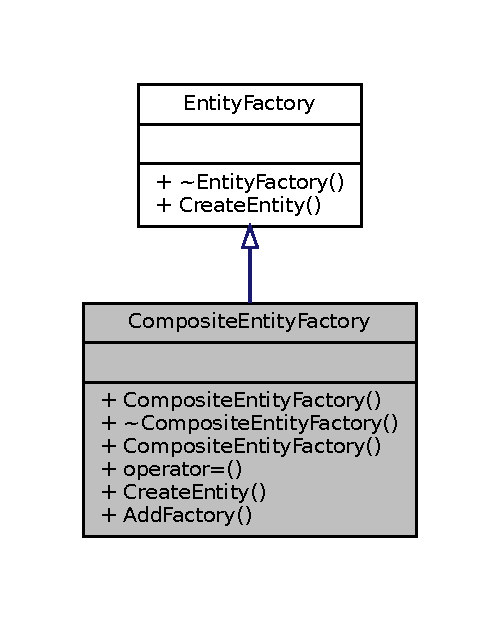
\includegraphics[width=240pt]{classCompositeEntityFactory__inherit__graph}
\end{center}
\end{figure}


Collaboration diagram for Composite\+Entity\+Factory\+:\nopagebreak
\begin{figure}[H]
\begin{center}
\leavevmode
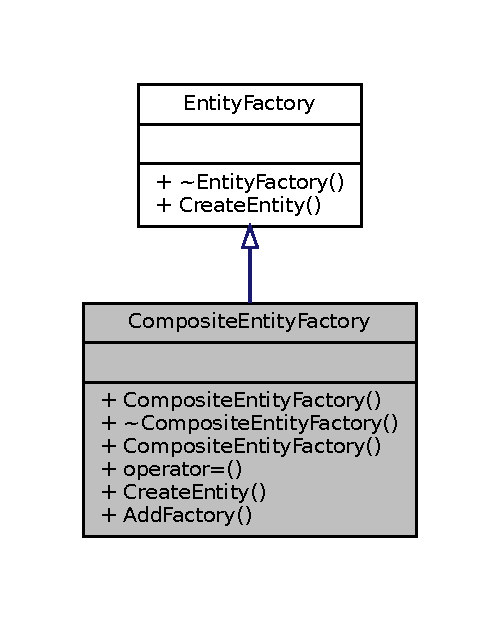
\includegraphics[width=240pt]{classCompositeEntityFactory__coll__graph}
\end{center}
\end{figure}
\subsection*{Public Member Functions}
\begin{DoxyCompactItemize}
\item 
\mbox{\Hypertarget{classCompositeEntityFactory_a703746f2b94fc98640de097afdbe1bc9}\label{classCompositeEntityFactory_a703746f2b94fc98640de097afdbe1bc9}} 
\hyperlink{classCompositeEntityFactory_a703746f2b94fc98640de097afdbe1bc9}{Composite\+Entity\+Factory} ()
\begin{DoxyCompactList}\small\item\em Default Constructor. \end{DoxyCompactList}\item 
\mbox{\Hypertarget{classCompositeEntityFactory_a62ec6ba774e3b397fc799c5e972dba45}\label{classCompositeEntityFactory_a62ec6ba774e3b397fc799c5e972dba45}} 
\hyperlink{classCompositeEntityFactory_a62ec6ba774e3b397fc799c5e972dba45}{$\sim$\+Composite\+Entity\+Factory} ()
\begin{DoxyCompactList}\small\item\em Destructor deleating all factories. \end{DoxyCompactList}\item 
\hyperlink{classCompositeEntityFactory_af70fe797d67a1526715369890b1fb136}{Composite\+Entity\+Factory} (const \hyperlink{classCompositeEntityFactory}{Composite\+Entity\+Factory} \&object\+To\+Copy)
\begin{DoxyCompactList}\small\item\em Copy Constructor. \end{DoxyCompactList}\item 
void \hyperlink{classCompositeEntityFactory_aa53621c622f2dbbf57dc8b3f698c1c59}{operator=} (const \hyperlink{classCompositeEntityFactory}{Composite\+Entity\+Factory} \&object\+To\+Copy)
\begin{DoxyCompactList}\small\item\em equality overload operator \end{DoxyCompactList}\item 
\hyperlink{classIEntity}{I\+Entity} $\ast$ \hyperlink{classCompositeEntityFactory_a97b2f95333369f946d0f3ab2116b5f19}{Create\+Entity} (picojson\+::object \&object, \hyperlink{classICameraController}{I\+Camera\+Controller} \&camera\+Controller)
\begin{DoxyCompactList}\small\item\em calls factories and creates the enitity based on the picson object \end{DoxyCompactList}\item 
void \hyperlink{classCompositeEntityFactory_a735c4e6bf789486468c4610f75688be2}{Add\+Factory} (\hyperlink{classEntityFactory}{Entity\+Factory} $\ast$factory)
\begin{DoxyCompactList}\small\item\em Entity\+Factoryadded to the collection of factories in this object. \end{DoxyCompactList}\end{DoxyCompactItemize}


\subsection{Constructor \& Destructor Documentation}
\mbox{\Hypertarget{classCompositeEntityFactory_af70fe797d67a1526715369890b1fb136}\label{classCompositeEntityFactory_af70fe797d67a1526715369890b1fb136}} 
\index{Composite\+Entity\+Factory@{Composite\+Entity\+Factory}!Composite\+Entity\+Factory@{Composite\+Entity\+Factory}}
\index{Composite\+Entity\+Factory@{Composite\+Entity\+Factory}!Composite\+Entity\+Factory@{Composite\+Entity\+Factory}}
\subsubsection{\texorpdfstring{Composite\+Entity\+Factory()}{CompositeEntityFactory()}}
{\footnotesize\ttfamily Composite\+Entity\+Factory\+::\+Composite\+Entity\+Factory (\begin{DoxyParamCaption}\item[{const \hyperlink{classCompositeEntityFactory}{Composite\+Entity\+Factory} \&}]{object\+To\+Copy }\end{DoxyParamCaption})\hspace{0.3cm}{\ttfamily [inline]}}



Copy Constructor. 


\begin{DoxyParams}[1]{Parameters}
\mbox{\tt in}  & {\em object\+To\+Copy} & \hyperlink{classCompositeEntityFactory}{Composite\+Entity\+Factory} to copy \\
\hline
\end{DoxyParams}


\subsection{Member Function Documentation}
\mbox{\Hypertarget{classCompositeEntityFactory_a735c4e6bf789486468c4610f75688be2}\label{classCompositeEntityFactory_a735c4e6bf789486468c4610f75688be2}} 
\index{Composite\+Entity\+Factory@{Composite\+Entity\+Factory}!Add\+Factory@{Add\+Factory}}
\index{Add\+Factory@{Add\+Factory}!Composite\+Entity\+Factory@{Composite\+Entity\+Factory}}
\subsubsection{\texorpdfstring{Add\+Factory()}{AddFactory()}}
{\footnotesize\ttfamily void Composite\+Entity\+Factory\+::\+Add\+Factory (\begin{DoxyParamCaption}\item[{\hyperlink{classEntityFactory}{Entity\+Factory} $\ast$}]{factory }\end{DoxyParamCaption})}



Entity\+Factoryadded to the collection of factories in this object. 


\begin{DoxyParams}[1]{Parameters}
\mbox{\tt in}  & {\em factory} & object factory that needs to be added \\
\hline
\end{DoxyParams}
\mbox{\Hypertarget{classCompositeEntityFactory_a97b2f95333369f946d0f3ab2116b5f19}\label{classCompositeEntityFactory_a97b2f95333369f946d0f3ab2116b5f19}} 
\index{Composite\+Entity\+Factory@{Composite\+Entity\+Factory}!Create\+Entity@{Create\+Entity}}
\index{Create\+Entity@{Create\+Entity}!Composite\+Entity\+Factory@{Composite\+Entity\+Factory}}
\subsubsection{\texorpdfstring{Create\+Entity()}{CreateEntity()}}
{\footnotesize\ttfamily \hyperlink{classIEntity}{I\+Entity} $\ast$ Composite\+Entity\+Factory\+::\+Create\+Entity (\begin{DoxyParamCaption}\item[{picojson\+::object \&}]{object,  }\item[{\hyperlink{classICameraController}{I\+Camera\+Controller} \&}]{camera\+Controller }\end{DoxyParamCaption})\hspace{0.3cm}{\ttfamily [virtual]}}



calls factories and creates the enitity based on the picson object 


\begin{DoxyParams}[1]{Parameters}
\mbox{\tt in}  & {\em object} & json object representing the entity that needs to be created\\
\hline
\end{DoxyParams}
\begin{DoxyReturn}{Returns}
entity based on parameter/argument created 
\end{DoxyReturn}


Implements \hyperlink{classEntityFactory_a7f579ca02f15935e6901e5c955c9726a}{Entity\+Factory}.

\mbox{\Hypertarget{classCompositeEntityFactory_aa53621c622f2dbbf57dc8b3f698c1c59}\label{classCompositeEntityFactory_aa53621c622f2dbbf57dc8b3f698c1c59}} 
\index{Composite\+Entity\+Factory@{Composite\+Entity\+Factory}!operator=@{operator=}}
\index{operator=@{operator=}!Composite\+Entity\+Factory@{Composite\+Entity\+Factory}}
\subsubsection{\texorpdfstring{operator=()}{operator=()}}
{\footnotesize\ttfamily void Composite\+Entity\+Factory\+::operator= (\begin{DoxyParamCaption}\item[{const \hyperlink{classCompositeEntityFactory}{Composite\+Entity\+Factory} \&}]{object\+To\+Copy }\end{DoxyParamCaption})}



equality overload operator 


\begin{DoxyParams}[1]{Parameters}
\mbox{\tt in}  & {\em object\+To\+Copy} & \hyperlink{classCompositeEntityFactory}{Composite\+Entity\+Factory} to copy \\
\hline
\end{DoxyParams}


The documentation for this class was generated from the following files\+:\begin{DoxyCompactItemize}
\item 
/home/user/repo/project/src/\+Factory/\hyperlink{CompositeEntityFactory_8h}{Composite\+Entity\+Factory.\+h}\item 
/home/user/repo/project/src/\+Factory/\hyperlink{CompositeEntityFactory_8cc}{Composite\+Entity\+Factory.\+cc}\end{DoxyCompactItemize}

\hypertarget{classConvolutionFilter}{}\section{Convolution\+Filter Class Reference}
\label{classConvolutionFilter}\index{Convolution\+Filter@{Convolution\+Filter}}


\hyperlink{classConvolutionFilter}{Convolution\+Filter} is an abstract \hyperlink{classFilter}{Filter} class with a convolution kernel. In order to compute the value of each pixel, surrounding pixels are multiplied by kernel values and then their values are added together.  




{\ttfamily \#include $<$convolution\+\_\+filter.\+h$>$}



Inheritance diagram for Convolution\+Filter\+:\nopagebreak
\begin{figure}[H]
\begin{center}
\leavevmode
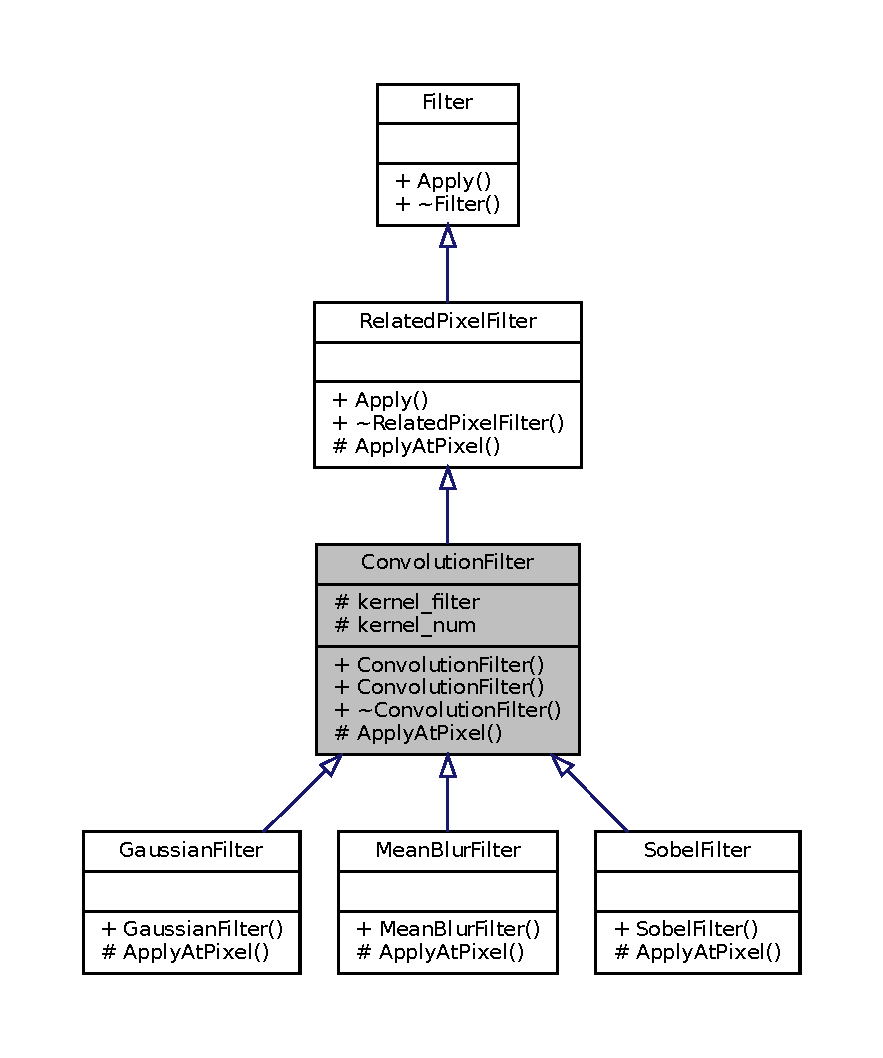
\includegraphics[width=350pt]{classConvolutionFilter__inherit__graph}
\end{center}
\end{figure}


Collaboration diagram for Convolution\+Filter\+:\nopagebreak
\begin{figure}[H]
\begin{center}
\leavevmode
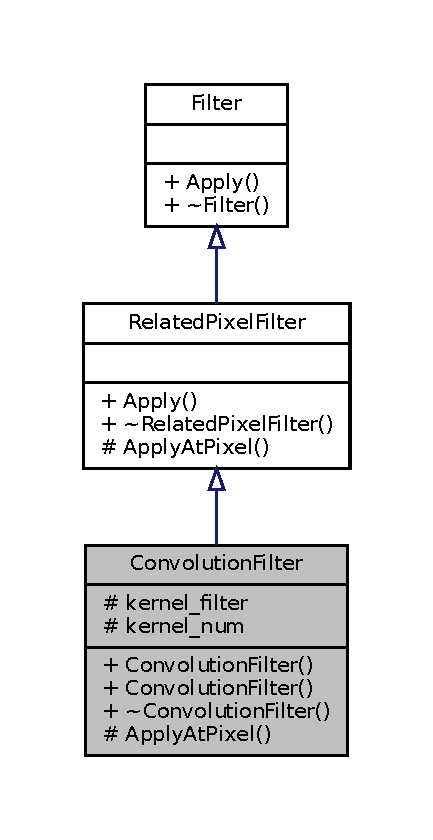
\includegraphics[width=208pt]{classConvolutionFilter__coll__graph}
\end{center}
\end{figure}
\subsection*{Public Member Functions}
\begin{DoxyCompactItemize}
\item 
\mbox{\Hypertarget{classConvolutionFilter_a7a92bc98d0d607a0be58874db37c3e1b}\label{classConvolutionFilter_a7a92bc98d0d607a0be58874db37c3e1b}} 
\hyperlink{classConvolutionFilter_a7a92bc98d0d607a0be58874db37c3e1b}{Convolution\+Filter} ()
\begin{DoxyCompactList}\small\item\em Empty convolution filter constructor. \end{DoxyCompactList}\item 
\hyperlink{classConvolutionFilter_af9356cfa9f768fbf7c97b51e7867ce12}{Convolution\+Filter} (std\+::unique\+\_\+ptr$<$ float\mbox{[}$\,$\mbox{]}$>$ matrix, int width, int height, int kernel\+\_\+num)
\begin{DoxyCompactList}\small\item\em Constructor of a Convolution \hyperlink{classFilter}{Filter} with a specified kernels. It is assumed that all kernels in the filter have the same dimensions. \end{DoxyCompactList}\item 
\mbox{\Hypertarget{classConvolutionFilter_a8d14d7b0f063528641be7fca0f1cd9dc}\label{classConvolutionFilter_a8d14d7b0f063528641be7fca0f1cd9dc}} 
virtual \hyperlink{classConvolutionFilter_a8d14d7b0f063528641be7fca0f1cd9dc}{$\sim$\+Convolution\+Filter} ()
\begin{DoxyCompactList}\small\item\em Virtual destructor that is needed for polymorphism since derived classes constructors need to be called. \end{DoxyCompactList}\end{DoxyCompactItemize}
\subsection*{Protected Member Functions}
\begin{DoxyCompactItemize}
\item 
virtual std\+::vector$<$ \hyperlink{classColor}{Color} $>$ \hyperlink{classConvolutionFilter_abc4b4ffef2b69fc2b7164e96af6cf186}{Apply\+At\+Pixel} (const std\+::vector$<$ \hyperlink{classImage}{Image} $\ast$$>$ original, int x, int y)=0
\begin{DoxyCompactList}\small\item\em Pure virtual method to apply the derived filter to one single pixel taking into consideration surrounding pixels. \end{DoxyCompactList}\end{DoxyCompactItemize}
\subsection*{Protected Attributes}
\begin{DoxyCompactItemize}
\item 
\mbox{\Hypertarget{classConvolutionFilter_ac78d47b9a00d813a527e48ccce62e7dc}\label{classConvolutionFilter_ac78d47b9a00d813a527e48ccce62e7dc}} 
std\+::vector$<$ \hyperlink{classKernel}{Kernel} $>$ {\bfseries kernel\+\_\+filter}
\item 
\mbox{\Hypertarget{classConvolutionFilter_aea4c4b00b3a15b3ba75ae2ce9ce141a2}\label{classConvolutionFilter_aea4c4b00b3a15b3ba75ae2ce9ce141a2}} 
int {\bfseries kernel\+\_\+num}
\end{DoxyCompactItemize}


\subsection{Detailed Description}
\hyperlink{classConvolutionFilter}{Convolution\+Filter} is an abstract \hyperlink{classFilter}{Filter} class with a convolution kernel. In order to compute the value of each pixel, surrounding pixels are multiplied by kernel values and then their values are added together. 

\subsection{Constructor \& Destructor Documentation}
\mbox{\Hypertarget{classConvolutionFilter_af9356cfa9f768fbf7c97b51e7867ce12}\label{classConvolutionFilter_af9356cfa9f768fbf7c97b51e7867ce12}} 
\index{Convolution\+Filter@{Convolution\+Filter}!Convolution\+Filter@{Convolution\+Filter}}
\index{Convolution\+Filter@{Convolution\+Filter}!Convolution\+Filter@{Convolution\+Filter}}
\subsubsection{\texorpdfstring{Convolution\+Filter()}{ConvolutionFilter()}}
{\footnotesize\ttfamily Convolution\+Filter\+::\+Convolution\+Filter (\begin{DoxyParamCaption}\item[{std\+::unique\+\_\+ptr$<$ float\mbox{[}$\,$\mbox{]}$>$}]{matrix,  }\item[{int}]{width,  }\item[{int}]{height,  }\item[{int}]{kernel\+\_\+num }\end{DoxyParamCaption})}



Constructor of a Convolution \hyperlink{classFilter}{Filter} with a specified kernels. It is assumed that all kernels in the filter have the same dimensions. 


\begin{DoxyParams}[1]{Parameters}
\mbox{\tt in}  & {\em matrix} & A float unique pointer array containing all the values of each of the kernels. \\
\hline
\mbox{\tt in}  & {\em width} & An integer value that represents the width of a kernel. \\
\hline
\mbox{\tt in}  & {\em height} & An integer value that represents the height of a kernel. \\
\hline
\mbox{\tt in}  & {\em kernel\+\_\+num} & An integer value that represents the number of a kernels that this convolution filter holds. \\
\hline
\end{DoxyParams}


\subsection{Member Function Documentation}
\mbox{\Hypertarget{classConvolutionFilter_abc4b4ffef2b69fc2b7164e96af6cf186}\label{classConvolutionFilter_abc4b4ffef2b69fc2b7164e96af6cf186}} 
\index{Convolution\+Filter@{Convolution\+Filter}!Apply\+At\+Pixel@{Apply\+At\+Pixel}}
\index{Apply\+At\+Pixel@{Apply\+At\+Pixel}!Convolution\+Filter@{Convolution\+Filter}}
\subsubsection{\texorpdfstring{Apply\+At\+Pixel()}{ApplyAtPixel()}}
{\footnotesize\ttfamily virtual std\+::vector$<$\hyperlink{classColor}{Color}$>$ Convolution\+Filter\+::\+Apply\+At\+Pixel (\begin{DoxyParamCaption}\item[{const std\+::vector$<$ \hyperlink{classImage}{Image} $\ast$$>$}]{original,  }\item[{int}]{x,  }\item[{int}]{y }\end{DoxyParamCaption})\hspace{0.3cm}{\ttfamily [protected]}, {\ttfamily [pure virtual]}}



Pure virtual method to apply the derived filter to one single pixel taking into consideration surrounding pixels. 


\begin{DoxyParams}[1]{Parameters}
\mbox{\tt in}  & {\em original} & A vector of input images to apply the filter over. \\
\hline
\mbox{\tt in}  & {\em x} & An integer representing the width in which the image color pixel is located, and the pixel to which the filter should be applied. \\
\hline
\mbox{\tt in}  & {\em x} & An integer representing the height in which the image color pixel is located, and the pixel to which the filter should be applied.\\
\hline
\end{DoxyParams}
\begin{DoxyReturn}{Returns}
A unique pointer array containing a color for each filtered image the filter should produce as an output 
\end{DoxyReturn}


Implements \hyperlink{classRelatedPixelFilter_a4701695c3b2ca7fdcc41b3d03c5840df}{Related\+Pixel\+Filter}.



Implemented in \hyperlink{classGaussianFilter_af8bf2d0f68642e6232f8b73ef1bee512}{Gaussian\+Filter}, \hyperlink{classSobelFilter_a7ce32ba94d87a008e7344863c442a1bb}{Sobel\+Filter}, and \hyperlink{classMeanBlurFilter_a59f554dae7213e726db9235979eef86b}{Mean\+Blur\+Filter}.



The documentation for this class was generated from the following files\+:\begin{DoxyCompactItemize}
\item 
/home/user/repo/project/\+Image\+Processing/\hyperlink{convolution__filter_8h}{convolution\+\_\+filter.\+h}\item 
/home/user/repo/project/\+Image\+Processing/\hyperlink{convolution__filter_8cc}{convolution\+\_\+filter.\+cc}\end{DoxyCompactItemize}

\hypertarget{classDataCollector}{}\section{Data\+Collector Class Reference}
\label{classDataCollector}\index{Data\+Collector@{Data\+Collector}}


A singleton class that collects and writes data to a C\+SV file.  




{\ttfamily \#include $<$Data\+Collector.\+h$>$}



Collaboration diagram for Data\+Collector\+:\nopagebreak
\begin{figure}[H]
\begin{center}
\leavevmode
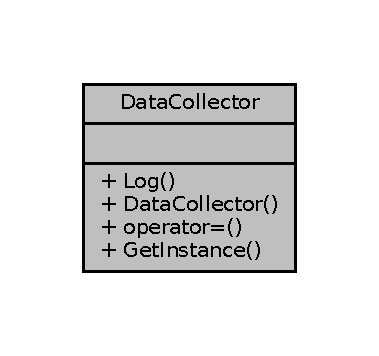
\includegraphics[width=182pt]{classDataCollector__coll__graph}
\end{center}
\end{figure}
\subsection*{Public Member Functions}
\begin{DoxyCompactItemize}
\item 
void \hyperlink{classDataCollector_af7d41172cc49dfb689ba91cf2171a5e8}{Log} (const std\+::string \&msg, bool overwrite)
\begin{DoxyCompactList}\small\item\em A function that takes in a message to write to the C\+SV file and a flag to control if the contents of the file are overwritten. \end{DoxyCompactList}\item 
\mbox{\Hypertarget{classDataCollector_a88476cb5acca163870167efd5179f253}\label{classDataCollector_a88476cb5acca163870167efd5179f253}} 
\hyperlink{classDataCollector_a88476cb5acca163870167efd5179f253}{Data\+Collector} (const \hyperlink{classDataCollector}{Data\+Collector} \&)=delete
\begin{DoxyCompactList}\small\item\em Delete copy constructor to keep \hyperlink{classDataCollector}{Data\+Collector} as a Singleton. \end{DoxyCompactList}\item 
\mbox{\Hypertarget{classDataCollector_a54763523f38fd4bd3f15b84a35ae8efb}\label{classDataCollector_a54763523f38fd4bd3f15b84a35ae8efb}} 
void \hyperlink{classDataCollector_a54763523f38fd4bd3f15b84a35ae8efb}{operator=} (const \hyperlink{classDataCollector}{Data\+Collector} \&)=delete
\begin{DoxyCompactList}\small\item\em Delete assignment operator to keep \hyperlink{classDataCollector}{Data\+Collector} as a Singleton. \end{DoxyCompactList}\end{DoxyCompactItemize}
\subsection*{Static Public Member Functions}
\begin{DoxyCompactItemize}
\item 
static \hyperlink{classDataCollector}{Data\+Collector} \& \hyperlink{classDataCollector_aa1cf25c127a7261ccaae4fac0fc5645b}{Get\+Instance} ()
\begin{DoxyCompactList}\small\item\em A static function that returns a reference to the single instance of the \hyperlink{classDataCollector}{Data\+Collector} class. \end{DoxyCompactList}\end{DoxyCompactItemize}


\subsection{Detailed Description}
A singleton class that collects and writes data to a C\+SV file. 

\subsection{Member Function Documentation}
\mbox{\Hypertarget{classDataCollector_aa1cf25c127a7261ccaae4fac0fc5645b}\label{classDataCollector_aa1cf25c127a7261ccaae4fac0fc5645b}} 
\index{Data\+Collector@{Data\+Collector}!Get\+Instance@{Get\+Instance}}
\index{Get\+Instance@{Get\+Instance}!Data\+Collector@{Data\+Collector}}
\subsubsection{\texorpdfstring{Get\+Instance()}{GetInstance()}}
{\footnotesize\ttfamily \hyperlink{classDataCollector}{Data\+Collector} \& Data\+Collector\+::\+Get\+Instance (\begin{DoxyParamCaption}{ }\end{DoxyParamCaption})\hspace{0.3cm}{\ttfamily [static]}}



A static function that returns a reference to the single instance of the \hyperlink{classDataCollector}{Data\+Collector} class. 

\begin{DoxyReturn}{Returns}
Returns a reference to the singel instace of the \hyperlink{classDataCollector}{Data\+Collector} class. 
\end{DoxyReturn}
\mbox{\Hypertarget{classDataCollector_af7d41172cc49dfb689ba91cf2171a5e8}\label{classDataCollector_af7d41172cc49dfb689ba91cf2171a5e8}} 
\index{Data\+Collector@{Data\+Collector}!Log@{Log}}
\index{Log@{Log}!Data\+Collector@{Data\+Collector}}
\subsubsection{\texorpdfstring{Log()}{Log()}}
{\footnotesize\ttfamily void Data\+Collector\+::\+Log (\begin{DoxyParamCaption}\item[{const std\+::string \&}]{msg,  }\item[{bool}]{overwrite }\end{DoxyParamCaption})}



A function that takes in a message to write to the C\+SV file and a flag to control if the contents of the file are overwritten. 


\begin{DoxyParams}[1]{Parameters}
\mbox{\tt in}  & {\em msg} & A constant reference to a string containing the comma separated values to write to the C\+SV file \\
\hline
\mbox{\tt in}  & {\em overwrite} & A boolean flag that determines if the contents of the C\+SV file should be overwritten before writing the new msg. \\
\hline
\end{DoxyParams}


The documentation for this class was generated from the following files\+:\begin{DoxyCompactItemize}
\item 
/home/user/repo/project/src/\+Data\+Collector/\hyperlink{DataCollector_8h}{Data\+Collector.\+h}\item 
/home/user/repo/project/src/\+Data\+Collector/\hyperlink{DataCollector_8cc}{Data\+Collector.\+cc}\end{DoxyCompactItemize}

\hypertarget{classDoubleThresholdFilter}{}\section{Double\+Threshold\+Filter Class Reference}
\label{classDoubleThresholdFilter}\index{Double\+Threshold\+Filter@{Double\+Threshold\+Filter}}


A class that can be used to apply a Double Threshold \hyperlink{classFilter}{Filter} to an \hyperlink{classImage}{Image}.  




{\ttfamily \#include $<$double\+\_\+threshold\+\_\+filter.\+h$>$}



Inheritance diagram for Double\+Threshold\+Filter\+:\nopagebreak
\begin{figure}[H]
\begin{center}
\leavevmode
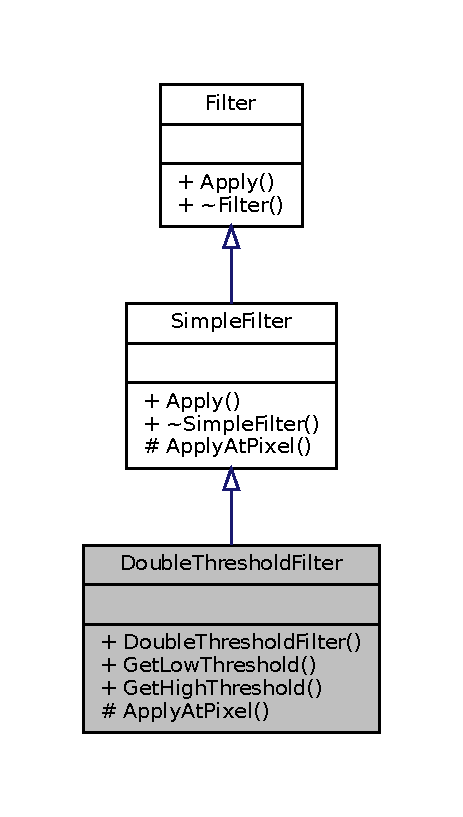
\includegraphics[width=222pt]{classDoubleThresholdFilter__inherit__graph}
\end{center}
\end{figure}


Collaboration diagram for Double\+Threshold\+Filter\+:\nopagebreak
\begin{figure}[H]
\begin{center}
\leavevmode
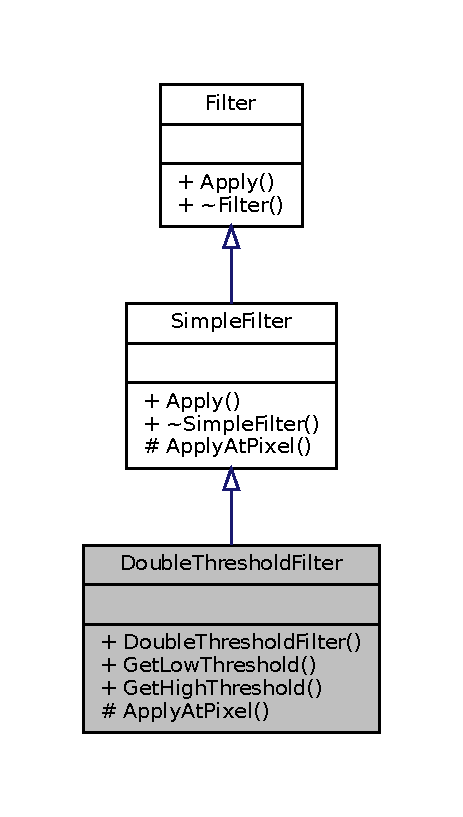
\includegraphics[width=222pt]{classDoubleThresholdFilter__coll__graph}
\end{center}
\end{figure}
\subsection*{Public Member Functions}
\begin{DoxyCompactItemize}
\item 
\hyperlink{classDoubleThresholdFilter_abd3b482cd8a1f554e819ced5fe36699f}{Double\+Threshold\+Filter} (float low\+Threshold\+Ratio, float high\+Threshold\+Ratio)
\begin{DoxyCompactList}\small\item\em Constructor of a Double Threshold \hyperlink{classFilter}{Filter} with a specified low-\/threshold and high-\/threshold. \end{DoxyCompactList}\item 
float \hyperlink{classDoubleThresholdFilter_a3417a9655273bcf69280aaee6666d25b}{Get\+Low\+Threshold} ()
\begin{DoxyCompactList}\small\item\em Get the value of the low-\/threshold for an instance of the \hyperlink{classDoubleThresholdFilter}{Double\+Threshold\+Filter} class. \end{DoxyCompactList}\item 
float \hyperlink{classDoubleThresholdFilter_aedbed79b6c46e2a8c76616294ee2be9d}{Get\+High\+Threshold} ()
\begin{DoxyCompactList}\small\item\em Get the value of the high-\/threshold for an instance of the \hyperlink{classDoubleThresholdFilter}{Double\+Threshold\+Filter} class. \end{DoxyCompactList}\end{DoxyCompactItemize}
\subsection*{Protected Member Functions}
\begin{DoxyCompactItemize}
\item 
\hyperlink{classColor}{Color} \hyperlink{classDoubleThresholdFilter_a1ae6e4b94ecfa8c9e978b5da897c136d}{Apply\+At\+Pixel} (const \hyperlink{classImage}{Image} $\ast$image, const \hyperlink{classColor}{Color} \&pixel)
\begin{DoxyCompactList}\small\item\em Modify the pixel of an image to apply the effects of a Double Threshold filter on that image. \end{DoxyCompactList}\end{DoxyCompactItemize}


\subsection{Detailed Description}
A class that can be used to apply a Double Threshold \hyperlink{classFilter}{Filter} to an \hyperlink{classImage}{Image}. 

\subsection{Constructor \& Destructor Documentation}
\mbox{\Hypertarget{classDoubleThresholdFilter_abd3b482cd8a1f554e819ced5fe36699f}\label{classDoubleThresholdFilter_abd3b482cd8a1f554e819ced5fe36699f}} 
\index{Double\+Threshold\+Filter@{Double\+Threshold\+Filter}!Double\+Threshold\+Filter@{Double\+Threshold\+Filter}}
\index{Double\+Threshold\+Filter@{Double\+Threshold\+Filter}!Double\+Threshold\+Filter@{Double\+Threshold\+Filter}}
\subsubsection{\texorpdfstring{Double\+Threshold\+Filter()}{DoubleThresholdFilter()}}
{\footnotesize\ttfamily Double\+Threshold\+Filter\+::\+Double\+Threshold\+Filter (\begin{DoxyParamCaption}\item[{float}]{low\+Threshold\+Ratio,  }\item[{float}]{high\+Threshold\+Ratio }\end{DoxyParamCaption})}



Constructor of a Double Threshold \hyperlink{classFilter}{Filter} with a specified low-\/threshold and high-\/threshold. 


\begin{DoxyParams}[1]{Parameters}
\mbox{\tt in}  & {\em low\+Threshold\+Ratio} & A float value that represents the low-\/threshold value. \\
\hline
\mbox{\tt in}  & {\em high\+Threshold\+Ratio} & A float value that represents the high-\/threshold value.\\
\hline
\end{DoxyParams}
\begin{DoxyReturn}{Returns}
Returns an instance of a \hyperlink{classDoubleThresholdFilter}{Double\+Threshold\+Filter} with the specified low-\/threshold and high-\/threshold values. 
\end{DoxyReturn}


\subsection{Member Function Documentation}
\mbox{\Hypertarget{classDoubleThresholdFilter_a1ae6e4b94ecfa8c9e978b5da897c136d}\label{classDoubleThresholdFilter_a1ae6e4b94ecfa8c9e978b5da897c136d}} 
\index{Double\+Threshold\+Filter@{Double\+Threshold\+Filter}!Apply\+At\+Pixel@{Apply\+At\+Pixel}}
\index{Apply\+At\+Pixel@{Apply\+At\+Pixel}!Double\+Threshold\+Filter@{Double\+Threshold\+Filter}}
\subsubsection{\texorpdfstring{Apply\+At\+Pixel()}{ApplyAtPixel()}}
{\footnotesize\ttfamily \hyperlink{classColor}{Color} Double\+Threshold\+Filter\+::\+Apply\+At\+Pixel (\begin{DoxyParamCaption}\item[{const \hyperlink{classImage}{Image} $\ast$}]{image,  }\item[{const \hyperlink{classColor}{Color} \&}]{pixel }\end{DoxyParamCaption})\hspace{0.3cm}{\ttfamily [protected]}, {\ttfamily [virtual]}}



Modify the pixel of an image to apply the effects of a Double Threshold filter on that image. 


\begin{DoxyParams}[1]{Parameters}
\mbox{\tt in}  & {\em image} & A constant pointer to an instance of the \hyperlink{classImage}{Image} class. \\
\hline
\mbox{\tt in}  & {\em pixel} & A reference to an instance of the \hyperlink{classColor}{Color} class that represents the pixel of an image to apply the Double Threshold filter to.\\
\hline
\end{DoxyParams}
\begin{DoxyReturn}{Returns}
Returns an instance of the \hyperlink{classColor}{Color} class representing the new \hyperlink{classColor}{Color} that the pixel in the image will be changed to after applying the Double Threshold filter. 
\end{DoxyReturn}


Implements \hyperlink{classSimpleFilter_aa12dc75dac8932ce03a9c9a3c7964b30}{Simple\+Filter}.

\mbox{\Hypertarget{classDoubleThresholdFilter_aedbed79b6c46e2a8c76616294ee2be9d}\label{classDoubleThresholdFilter_aedbed79b6c46e2a8c76616294ee2be9d}} 
\index{Double\+Threshold\+Filter@{Double\+Threshold\+Filter}!Get\+High\+Threshold@{Get\+High\+Threshold}}
\index{Get\+High\+Threshold@{Get\+High\+Threshold}!Double\+Threshold\+Filter@{Double\+Threshold\+Filter}}
\subsubsection{\texorpdfstring{Get\+High\+Threshold()}{GetHighThreshold()}}
{\footnotesize\ttfamily float Double\+Threshold\+Filter\+::\+Get\+High\+Threshold (\begin{DoxyParamCaption}{ }\end{DoxyParamCaption})}



Get the value of the high-\/threshold for an instance of the \hyperlink{classDoubleThresholdFilter}{Double\+Threshold\+Filter} class. 

\begin{DoxyReturn}{Returns}
Returns an a float containing the value of the high-\/threshold set for this Double Threshold filter. 
\end{DoxyReturn}
\mbox{\Hypertarget{classDoubleThresholdFilter_a3417a9655273bcf69280aaee6666d25b}\label{classDoubleThresholdFilter_a3417a9655273bcf69280aaee6666d25b}} 
\index{Double\+Threshold\+Filter@{Double\+Threshold\+Filter}!Get\+Low\+Threshold@{Get\+Low\+Threshold}}
\index{Get\+Low\+Threshold@{Get\+Low\+Threshold}!Double\+Threshold\+Filter@{Double\+Threshold\+Filter}}
\subsubsection{\texorpdfstring{Get\+Low\+Threshold()}{GetLowThreshold()}}
{\footnotesize\ttfamily float Double\+Threshold\+Filter\+::\+Get\+Low\+Threshold (\begin{DoxyParamCaption}{ }\end{DoxyParamCaption})}



Get the value of the low-\/threshold for an instance of the \hyperlink{classDoubleThresholdFilter}{Double\+Threshold\+Filter} class. 

\begin{DoxyReturn}{Returns}
Returns an a float containing the value of the low-\/threshold set for this Double Threshold filter. 
\end{DoxyReturn}


The documentation for this class was generated from the following files\+:\begin{DoxyCompactItemize}
\item 
/home/user/repo/project/\+Image\+Processing/\hyperlink{double__threshold__filter_8h}{double\+\_\+threshold\+\_\+filter.\+h}\item 
/home/user/repo/project/\+Image\+Processing/\hyperlink{double__threshold__filter_8cc}{double\+\_\+threshold\+\_\+filter.\+cc}\end{DoxyCompactItemize}

\hypertarget{classDrone}{}\section{Drone Class Reference}
\label{classDrone}\index{Drone@{Drone}}


Inheritance diagram for Drone\+:\nopagebreak
\begin{figure}[H]
\begin{center}
\leavevmode
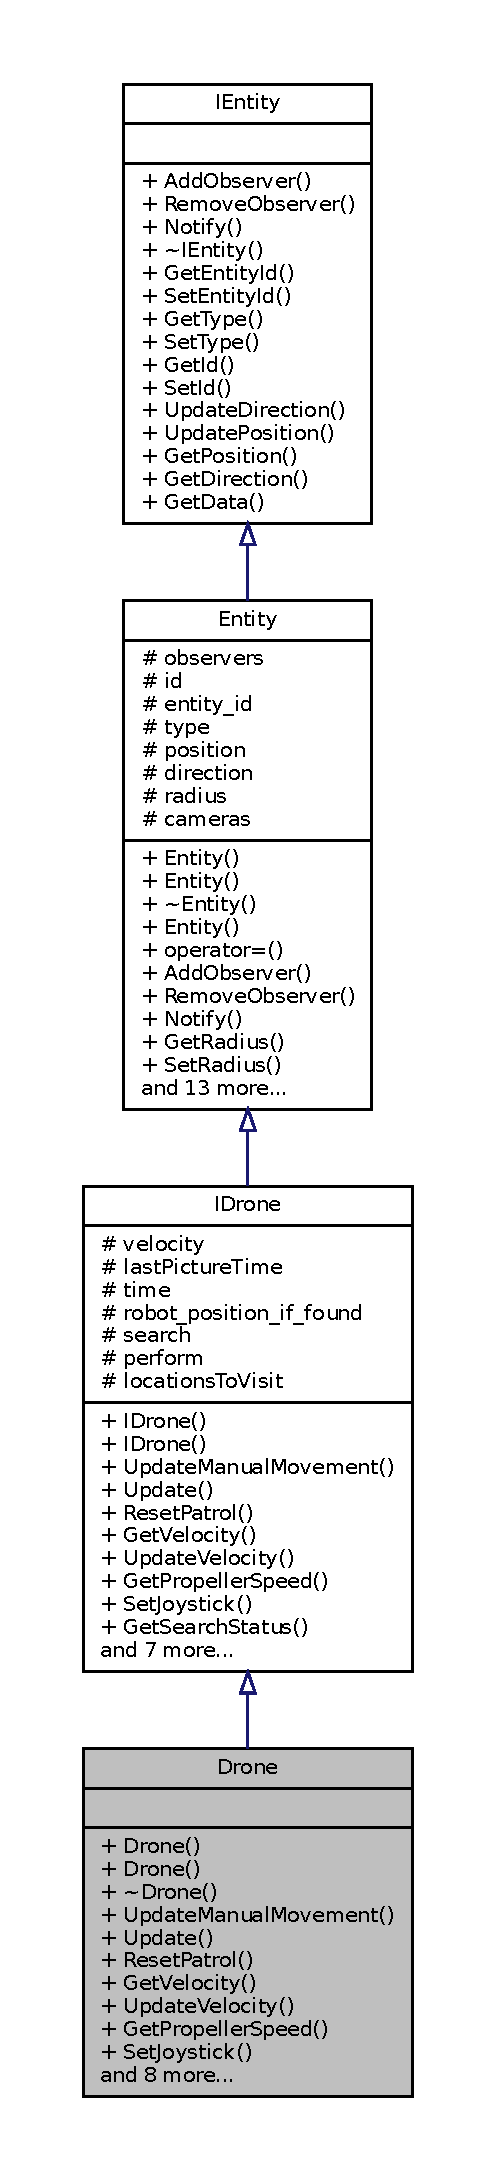
\includegraphics[height=550pt]{classDrone__inherit__graph}
\end{center}
\end{figure}


Collaboration diagram for Drone\+:\nopagebreak
\begin{figure}[H]
\begin{center}
\leavevmode
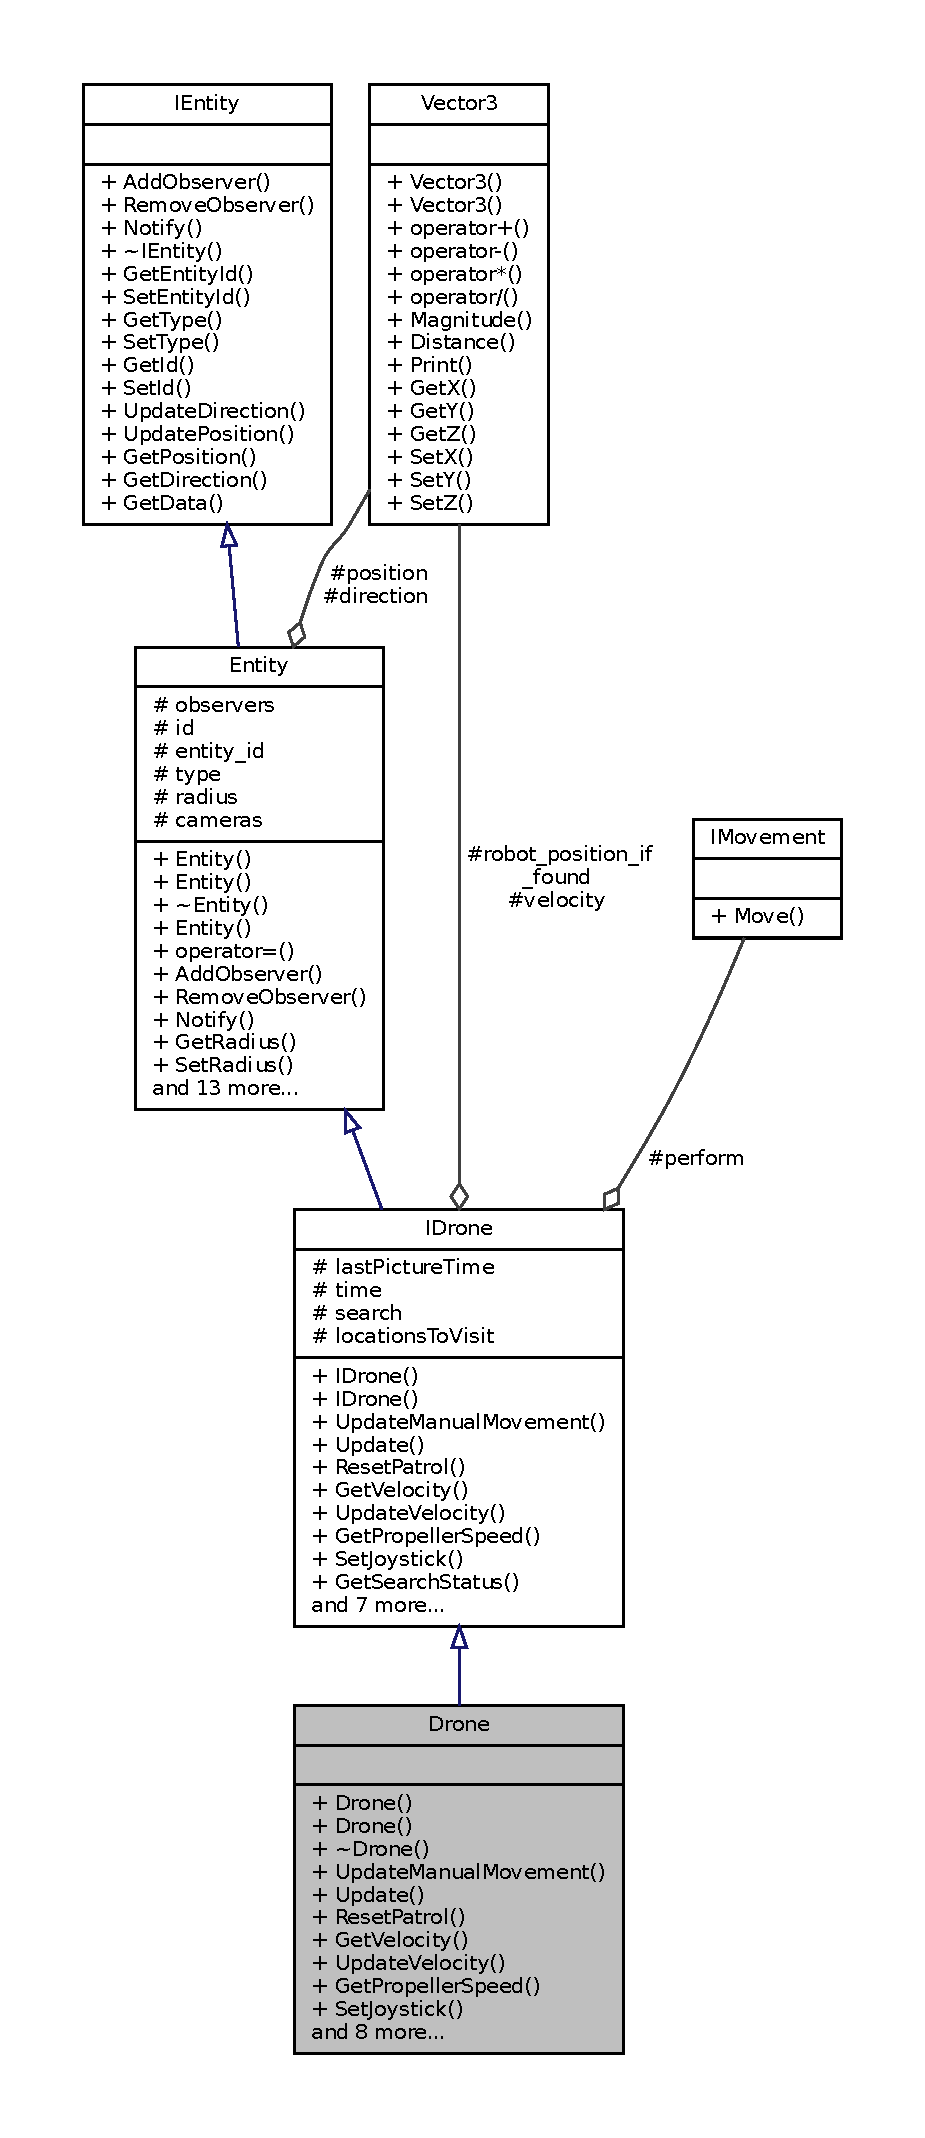
\includegraphics[height=550pt]{classDrone__coll__graph}
\end{center}
\end{figure}
\subsection*{Public Member Functions}
\begin{DoxyCompactItemize}
\item 
\mbox{\Hypertarget{classDrone_ab692baa4be5c43b72990ce1b01bdc805}\label{classDrone_ab692baa4be5c43b72990ce1b01bdc805}} 
\hyperlink{classDrone_ab692baa4be5c43b72990ce1b01bdc805}{Drone} ()
\begin{DoxyCompactList}\small\item\em empty constructor \end{DoxyCompactList}\item 
\hyperlink{classDrone_a4f426cef8328894a819cc31ba4b2bcdb}{Drone} (picojson\+::object \&obj)
\begin{DoxyCompactList}\small\item\em Constructor. \end{DoxyCompactList}\item 
\mbox{\Hypertarget{classDrone_a667075abb1eb5c54be6418884a387d14}\label{classDrone_a667075abb1eb5c54be6418884a387d14}} 
\hyperlink{classDrone_a667075abb1eb5c54be6418884a387d14}{$\sim$\+Drone} ()
\begin{DoxyCompactList}\small\item\em A destructor for all \hyperlink{classDrone}{Drone} instances. \end{DoxyCompactList}\item 
void \hyperlink{classDrone_aabfc6155cd0b8e14ae77c4659c090185}{Update\+Manual\+Movement} (double dt)
\begin{DoxyCompactList}\small\item\em Moves based on keyboard inputs. \end{DoxyCompactList}\item 
void \hyperlink{classDrone_abc6b79ccc7fdbc3bec8d539fc836c04d}{Update} (double dt)
\begin{DoxyCompactList}\small\item\em Calculates the new position of the drone based on Euler´s integration. \end{DoxyCompactList}\item 
\mbox{\Hypertarget{classDrone_a02b047f6ed0d4e95df1b3efb4a7ce9bc}\label{classDrone_a02b047f6ed0d4e95df1b3efb4a7ce9bc}} 
void \hyperlink{classDrone_a02b047f6ed0d4e95df1b3efb4a7ce9bc}{Reset\+Patrol} ()
\begin{DoxyCompactList}\small\item\em Calculates the new patrol movement if we are still searching for the robot and have switch between manual and automatic movement. \end{DoxyCompactList}\item 
\hyperlink{classVector3}{Vector3} \hyperlink{classDrone_ac5adae4a3cbe2e39f577fa7da14407c7}{Get\+Velocity} () const
\begin{DoxyCompactList}\small\item\em getter for the velocity of the drone \end{DoxyCompactList}\item 
void \hyperlink{classDrone_a8ecc9a70f1d3907a79be433bfa9b5d68}{Update\+Velocity} (const \hyperlink{classVector3}{Vector3} \&new\+Dir)
\begin{DoxyCompactList}\small\item\em Updates the velocity of the drone. \end{DoxyCompactList}\item 
double \hyperlink{classDrone_a7b2fd7d3ed57cec48ebdcd09f97b83f7}{Get\+Propeller\+Speed} (int index)
\begin{DoxyCompactList}\small\item\em getter for the speed of one of the legs of the drone \end{DoxyCompactList}\item 
void \hyperlink{classDrone_a648ebd16d398c677918d94471010ddc6}{Set\+Joystick} (double x, double y, double z, double rotate)
\begin{DoxyCompactList}\small\item\em setter for the direction of the drone based on manual movement \end{DoxyCompactList}\item 
bool \hyperlink{classDrone_a9bfe1ce0aea1215da3072434ed8e8527}{Get\+Search\+Status} () const
\begin{DoxyCompactList}\small\item\em getter for the state of drone´s search (robot found or Not) \end{DoxyCompactList}\item 
void \hyperlink{classDrone_a5349ad4b562b038a2d27ede3ed3fa80d}{Set\+Search\+Status} (bool status)
\begin{DoxyCompactList}\small\item\em setter for the state of drone´s search (robot found or Not) \end{DoxyCompactList}\item 
float \hyperlink{classDrone_a78de3dcbc6ae754e8874a8b65e8cd9ee}{Get\+Last\+Picture\+Time} () const
\begin{DoxyCompactList}\small\item\em getter for the last time drone took a pic \end{DoxyCompactList}\item 
void \hyperlink{classDrone_af639374e11eb02702665ba9f71697a01}{Set\+Last\+Picture\+Time} (float time\+Pic)
\begin{DoxyCompactList}\small\item\em setter for the last time drone took a pic \end{DoxyCompactList}\item 
float \hyperlink{classDrone_a0fde6a9a239da64ae102053c6404fe4d}{Get\+Time} () const
\begin{DoxyCompactList}\small\item\em getter for the time elapsed \end{DoxyCompactList}\item 
void \hyperlink{classDrone_a3c8e1ccbff90c7b5192679317f219061}{Set\+Time} (float t)
\begin{DoxyCompactList}\small\item\em setter for the time elapsed \end{DoxyCompactList}\item 
\hyperlink{classVector3}{Vector3} \hyperlink{classDrone_afdba5de8493255a433d62382991dfe8e}{Get\+Robot\+Pos} () const
\begin{DoxyCompactList}\small\item\em A method to get the robot x y z position. \end{DoxyCompactList}\item 
void \hyperlink{classDrone_a384abec1f84c15ec1c5533d9ccc8b865}{Set\+Robot\+Pos} (\hyperlink{classVector3}{Vector3} pos)
\begin{DoxyCompactList}\small\item\em A method to set the robot x y z position. \end{DoxyCompactList}\end{DoxyCompactItemize}
\subsection*{Additional Inherited Members}


\subsection{Constructor \& Destructor Documentation}
\mbox{\Hypertarget{classDrone_a4f426cef8328894a819cc31ba4b2bcdb}\label{classDrone_a4f426cef8328894a819cc31ba4b2bcdb}} 
\index{Drone@{Drone}!Drone@{Drone}}
\index{Drone@{Drone}!Drone@{Drone}}
\subsubsection{\texorpdfstring{Drone()}{Drone()}}
{\footnotesize\ttfamily Drone\+::\+Drone (\begin{DoxyParamCaption}\item[{picojson\+::object \&}]{obj }\end{DoxyParamCaption})\hspace{0.3cm}{\ttfamily [inline]}}



Constructor. 


\begin{DoxyParams}[1]{Parameters}
\mbox{\tt in}  & {\em object} & picson object Object that we want to retrive info from \\
\hline
\end{DoxyParams}


\subsection{Member Function Documentation}
\mbox{\Hypertarget{classDrone_a78de3dcbc6ae754e8874a8b65e8cd9ee}\label{classDrone_a78de3dcbc6ae754e8874a8b65e8cd9ee}} 
\index{Drone@{Drone}!Get\+Last\+Picture\+Time@{Get\+Last\+Picture\+Time}}
\index{Get\+Last\+Picture\+Time@{Get\+Last\+Picture\+Time}!Drone@{Drone}}
\subsubsection{\texorpdfstring{Get\+Last\+Picture\+Time()}{GetLastPictureTime()}}
{\footnotesize\ttfamily float Drone\+::\+Get\+Last\+Picture\+Time (\begin{DoxyParamCaption}{ }\end{DoxyParamCaption}) const\hspace{0.3cm}{\ttfamily [virtual]}}



getter for the last time drone took a pic 

\begin{DoxyReturn}{Returns}
float representing time elapsed since that picture 
\end{DoxyReturn}


Implements \hyperlink{classIDrone_a112d19971ac7d94dba9e2f25ad667c0d}{I\+Drone}.

\mbox{\Hypertarget{classDrone_a7b2fd7d3ed57cec48ebdcd09f97b83f7}\label{classDrone_a7b2fd7d3ed57cec48ebdcd09f97b83f7}} 
\index{Drone@{Drone}!Get\+Propeller\+Speed@{Get\+Propeller\+Speed}}
\index{Get\+Propeller\+Speed@{Get\+Propeller\+Speed}!Drone@{Drone}}
\subsubsection{\texorpdfstring{Get\+Propeller\+Speed()}{GetPropellerSpeed()}}
{\footnotesize\ttfamily double Drone\+::\+Get\+Propeller\+Speed (\begin{DoxyParamCaption}\item[{int}]{index }\end{DoxyParamCaption})\hspace{0.3cm}{\ttfamily [virtual]}}



getter for the speed of one of the legs of the drone 

\begin{DoxyReturn}{Returns}
double representing the speed of the index propeller 
\end{DoxyReturn}


Implements \hyperlink{classIDrone_a60a9a7eb90bf13100d66cb47b99830ed}{I\+Drone}.

\mbox{\Hypertarget{classDrone_afdba5de8493255a433d62382991dfe8e}\label{classDrone_afdba5de8493255a433d62382991dfe8e}} 
\index{Drone@{Drone}!Get\+Robot\+Pos@{Get\+Robot\+Pos}}
\index{Get\+Robot\+Pos@{Get\+Robot\+Pos}!Drone@{Drone}}
\subsubsection{\texorpdfstring{Get\+Robot\+Pos()}{GetRobotPos()}}
{\footnotesize\ttfamily \hyperlink{classVector3}{Vector3} Drone\+::\+Get\+Robot\+Pos (\begin{DoxyParamCaption}{ }\end{DoxyParamCaption}) const\hspace{0.3cm}{\ttfamily [virtual]}}



A method to get the robot x y z position. 

\begin{DoxyReturn}{Returns}
Vector representing position where robot found 
\end{DoxyReturn}


Implements \hyperlink{classIDrone_a1c3f5e712a97625c74c35952b930d68d}{I\+Drone}.

\mbox{\Hypertarget{classDrone_a9bfe1ce0aea1215da3072434ed8e8527}\label{classDrone_a9bfe1ce0aea1215da3072434ed8e8527}} 
\index{Drone@{Drone}!Get\+Search\+Status@{Get\+Search\+Status}}
\index{Get\+Search\+Status@{Get\+Search\+Status}!Drone@{Drone}}
\subsubsection{\texorpdfstring{Get\+Search\+Status()}{GetSearchStatus()}}
{\footnotesize\ttfamily bool Drone\+::\+Get\+Search\+Status (\begin{DoxyParamCaption}{ }\end{DoxyParamCaption}) const\hspace{0.3cm}{\ttfamily [virtual]}}



getter for the state of drone´s search (robot found or Not) 

\begin{DoxyReturn}{Returns}
boolean true if we have found robot and are moving torwards it, false otherwise 
\end{DoxyReturn}


Implements \hyperlink{classIDrone_aed9abde2152408ef3483da57f24c4006}{I\+Drone}.

\mbox{\Hypertarget{classDrone_a0fde6a9a239da64ae102053c6404fe4d}\label{classDrone_a0fde6a9a239da64ae102053c6404fe4d}} 
\index{Drone@{Drone}!Get\+Time@{Get\+Time}}
\index{Get\+Time@{Get\+Time}!Drone@{Drone}}
\subsubsection{\texorpdfstring{Get\+Time()}{GetTime()}}
{\footnotesize\ttfamily float Drone\+::\+Get\+Time (\begin{DoxyParamCaption}{ }\end{DoxyParamCaption}) const\hspace{0.3cm}{\ttfamily [virtual]}}



getter for the time elapsed 

\begin{DoxyReturn}{Returns}
float representing time elapsed (sum of updates dt´s) 
\end{DoxyReturn}


Implements \hyperlink{classIDrone_a18809d1b0626ba66984ef3a91ffb644c}{I\+Drone}.

\mbox{\Hypertarget{classDrone_ac5adae4a3cbe2e39f577fa7da14407c7}\label{classDrone_ac5adae4a3cbe2e39f577fa7da14407c7}} 
\index{Drone@{Drone}!Get\+Velocity@{Get\+Velocity}}
\index{Get\+Velocity@{Get\+Velocity}!Drone@{Drone}}
\subsubsection{\texorpdfstring{Get\+Velocity()}{GetVelocity()}}
{\footnotesize\ttfamily \hyperlink{classVector3}{Vector3} Drone\+::\+Get\+Velocity (\begin{DoxyParamCaption}{ }\end{DoxyParamCaption}) const\hspace{0.3cm}{\ttfamily [virtual]}}



getter for the velocity of the drone 

\begin{DoxyReturn}{Returns}
vector3 representing the velocity of the drone 
\end{DoxyReturn}


Implements \hyperlink{classIDrone_abad6c0adb60d6deceb13f30687fed57b}{I\+Drone}.

\mbox{\Hypertarget{classDrone_a648ebd16d398c677918d94471010ddc6}\label{classDrone_a648ebd16d398c677918d94471010ddc6}} 
\index{Drone@{Drone}!Set\+Joystick@{Set\+Joystick}}
\index{Set\+Joystick@{Set\+Joystick}!Drone@{Drone}}
\subsubsection{\texorpdfstring{Set\+Joystick()}{SetJoystick()}}
{\footnotesize\ttfamily void Drone\+::\+Set\+Joystick (\begin{DoxyParamCaption}\item[{double}]{x,  }\item[{double}]{y,  }\item[{double}]{z,  }\item[{double}]{rotate }\end{DoxyParamCaption})\hspace{0.3cm}{\ttfamily [virtual]}}



setter for the direction of the drone based on manual movement 


\begin{DoxyParams}[1]{Parameters}
\mbox{\tt in}  & {\em x} & double representing the direction on the x direction \\
\hline
\mbox{\tt in}  & {\em y} & double representing the direction on the y direction \\
\hline
\mbox{\tt in}  & {\em z} & double representing the direction on the z direction \\
\hline
\mbox{\tt in}  & {\em rotate} & double representing the rotation value of drone \\
\hline
\end{DoxyParams}


Implements \hyperlink{classIDrone_a8414edd320f25869fb04a880eae0d554}{I\+Drone}.

\mbox{\Hypertarget{classDrone_af639374e11eb02702665ba9f71697a01}\label{classDrone_af639374e11eb02702665ba9f71697a01}} 
\index{Drone@{Drone}!Set\+Last\+Picture\+Time@{Set\+Last\+Picture\+Time}}
\index{Set\+Last\+Picture\+Time@{Set\+Last\+Picture\+Time}!Drone@{Drone}}
\subsubsection{\texorpdfstring{Set\+Last\+Picture\+Time()}{SetLastPictureTime()}}
{\footnotesize\ttfamily void Drone\+::\+Set\+Last\+Picture\+Time (\begin{DoxyParamCaption}\item[{float}]{time\+Pic }\end{DoxyParamCaption})\hspace{0.3cm}{\ttfamily [virtual]}}



setter for the last time drone took a pic 


\begin{DoxyParams}[1]{Parameters}
\mbox{\tt in}  & {\em time\+Pic} & float representing time since last\+Picture \\
\hline
\end{DoxyParams}


Implements \hyperlink{classIDrone_aace45f6d9a77bfc8c61bd0ffc30a3b8e}{I\+Drone}.

\mbox{\Hypertarget{classDrone_a384abec1f84c15ec1c5533d9ccc8b865}\label{classDrone_a384abec1f84c15ec1c5533d9ccc8b865}} 
\index{Drone@{Drone}!Set\+Robot\+Pos@{Set\+Robot\+Pos}}
\index{Set\+Robot\+Pos@{Set\+Robot\+Pos}!Drone@{Drone}}
\subsubsection{\texorpdfstring{Set\+Robot\+Pos()}{SetRobotPos()}}
{\footnotesize\ttfamily void Drone\+::\+Set\+Robot\+Pos (\begin{DoxyParamCaption}\item[{\hyperlink{classVector3}{Vector3}}]{pos }\end{DoxyParamCaption})\hspace{0.3cm}{\ttfamily [virtual]}}



A method to set the robot x y z position. 


\begin{DoxyParams}[1]{Parameters}
\mbox{\tt in}  & {\em pos} & Vector representing position where robot found \\
\hline
\end{DoxyParams}


Implements \hyperlink{classIDrone_a5851e679bf3c915e93165377cb5c8815}{I\+Drone}.

\mbox{\Hypertarget{classDrone_a5349ad4b562b038a2d27ede3ed3fa80d}\label{classDrone_a5349ad4b562b038a2d27ede3ed3fa80d}} 
\index{Drone@{Drone}!Set\+Search\+Status@{Set\+Search\+Status}}
\index{Set\+Search\+Status@{Set\+Search\+Status}!Drone@{Drone}}
\subsubsection{\texorpdfstring{Set\+Search\+Status()}{SetSearchStatus()}}
{\footnotesize\ttfamily void Drone\+::\+Set\+Search\+Status (\begin{DoxyParamCaption}\item[{bool}]{status }\end{DoxyParamCaption})\hspace{0.3cm}{\ttfamily [virtual]}}



setter for the state of drone´s search (robot found or Not) 


\begin{DoxyParams}[1]{Parameters}
\mbox{\tt in}  & {\em status} & boolean true if we have found robot and are moving torwards it, false otherwise \\
\hline
\end{DoxyParams}


Implements \hyperlink{classIDrone_ac6f580814e7091ea64ecf2a7137b8120}{I\+Drone}.

\mbox{\Hypertarget{classDrone_a3c8e1ccbff90c7b5192679317f219061}\label{classDrone_a3c8e1ccbff90c7b5192679317f219061}} 
\index{Drone@{Drone}!Set\+Time@{Set\+Time}}
\index{Set\+Time@{Set\+Time}!Drone@{Drone}}
\subsubsection{\texorpdfstring{Set\+Time()}{SetTime()}}
{\footnotesize\ttfamily void Drone\+::\+Set\+Time (\begin{DoxyParamCaption}\item[{float}]{t }\end{DoxyParamCaption})\hspace{0.3cm}{\ttfamily [virtual]}}



setter for the time elapsed 


\begin{DoxyParams}[1]{Parameters}
\mbox{\tt in}  & {\em t} & float representing time elapsed (sum of updates dt´s) \\
\hline
\end{DoxyParams}


Implements \hyperlink{classIDrone_a0ca36885fd79fbf2efa3909771218d56}{I\+Drone}.

\mbox{\Hypertarget{classDrone_abc6b79ccc7fdbc3bec8d539fc836c04d}\label{classDrone_abc6b79ccc7fdbc3bec8d539fc836c04d}} 
\index{Drone@{Drone}!Update@{Update}}
\index{Update@{Update}!Drone@{Drone}}
\subsubsection{\texorpdfstring{Update()}{Update()}}
{\footnotesize\ttfamily void Drone\+::\+Update (\begin{DoxyParamCaption}\item[{double}]{dt }\end{DoxyParamCaption})\hspace{0.3cm}{\ttfamily [virtual]}}



Calculates the new position of the drone based on Euler´s integration. 


\begin{DoxyParams}[1]{Parameters}
\mbox{\tt in}  & {\em dt} & period of time it has elapsed since last update \\
\hline
\end{DoxyParams}


Implements \hyperlink{classIDrone_a6d840d60cda9a985b94af42ef54520b7}{I\+Drone}.

\mbox{\Hypertarget{classDrone_aabfc6155cd0b8e14ae77c4659c090185}\label{classDrone_aabfc6155cd0b8e14ae77c4659c090185}} 
\index{Drone@{Drone}!Update\+Manual\+Movement@{Update\+Manual\+Movement}}
\index{Update\+Manual\+Movement@{Update\+Manual\+Movement}!Drone@{Drone}}
\subsubsection{\texorpdfstring{Update\+Manual\+Movement()}{UpdateManualMovement()}}
{\footnotesize\ttfamily void Drone\+::\+Update\+Manual\+Movement (\begin{DoxyParamCaption}\item[{double}]{dt }\end{DoxyParamCaption})\hspace{0.3cm}{\ttfamily [virtual]}}



Moves based on keyboard inputs. 


\begin{DoxyParams}[1]{Parameters}
\mbox{\tt in}  & {\em dt} & period of time it has elapsed since last update \\
\hline
\end{DoxyParams}


Implements \hyperlink{classIDrone_a82486b4192f6ccf8b3d93fbb9101f2dd}{I\+Drone}.

\mbox{\Hypertarget{classDrone_a8ecc9a70f1d3907a79be433bfa9b5d68}\label{classDrone_a8ecc9a70f1d3907a79be433bfa9b5d68}} 
\index{Drone@{Drone}!Update\+Velocity@{Update\+Velocity}}
\index{Update\+Velocity@{Update\+Velocity}!Drone@{Drone}}
\subsubsection{\texorpdfstring{Update\+Velocity()}{UpdateVelocity()}}
{\footnotesize\ttfamily void Drone\+::\+Update\+Velocity (\begin{DoxyParamCaption}\item[{const \hyperlink{classVector3}{Vector3} \&}]{new\+Dir }\end{DoxyParamCaption})\hspace{0.3cm}{\ttfamily [virtual]}}



Updates the velocity of the drone. 


\begin{DoxyParams}[1]{Parameters}
\mbox{\tt in}  & {\em new\+Dir} & vector3 representing the new velocity of the object \\
\hline
\end{DoxyParams}


Implements \hyperlink{classIDrone_a5cc88b8205adaeea8f71c822d08e1607}{I\+Drone}.



The documentation for this class was generated from the following files\+:\begin{DoxyCompactItemize}
\item 
/home/user/repo/project/src/\+Entity/\hyperlink{Drone_8h}{Drone.\+h}\item 
/home/user/repo/project/src/\+Entity/\hyperlink{Drone_8cc}{Drone.\+cc}\end{DoxyCompactItemize}

\hypertarget{classDroneFactory}{}\section{Drone\+Factory Class Reference}
\label{classDroneFactory}\index{Drone\+Factory@{Drone\+Factory}}


Inheritance diagram for Drone\+Factory\+:\nopagebreak
\begin{figure}[H]
\begin{center}
\leavevmode
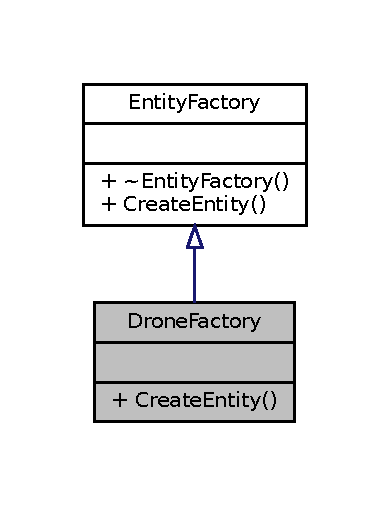
\includegraphics[width=187pt]{classDroneFactory__inherit__graph}
\end{center}
\end{figure}


Collaboration diagram for Drone\+Factory\+:\nopagebreak
\begin{figure}[H]
\begin{center}
\leavevmode
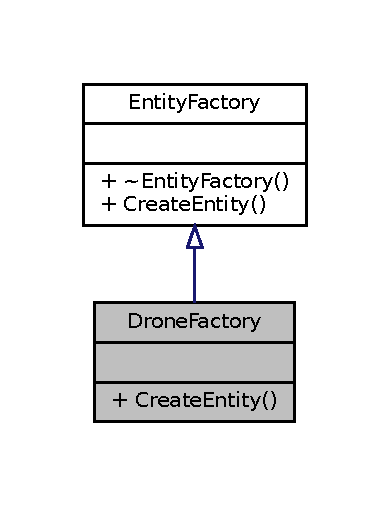
\includegraphics[width=187pt]{classDroneFactory__coll__graph}
\end{center}
\end{figure}
\subsection*{Public Member Functions}
\begin{DoxyCompactItemize}
\item 
\hyperlink{classIEntity}{I\+Entity} $\ast$ \hyperlink{classDroneFactory_a058b7be67ed594854ab9605236fa5c7e}{Create\+Entity} (picojson\+::object \&object, \hyperlink{classICameraController}{I\+Camera\+Controller} \&camera\+Controller)
\begin{DoxyCompactList}\small\item\em creates a \hyperlink{classDrone}{Drone} entity based on the picson object \end{DoxyCompactList}\end{DoxyCompactItemize}


\subsection{Member Function Documentation}
\mbox{\Hypertarget{classDroneFactory_a058b7be67ed594854ab9605236fa5c7e}\label{classDroneFactory_a058b7be67ed594854ab9605236fa5c7e}} 
\index{Drone\+Factory@{Drone\+Factory}!Create\+Entity@{Create\+Entity}}
\index{Create\+Entity@{Create\+Entity}!Drone\+Factory@{Drone\+Factory}}
\subsubsection{\texorpdfstring{Create\+Entity()}{CreateEntity()}}
{\footnotesize\ttfamily \hyperlink{classIEntity}{I\+Entity} $\ast$ Drone\+Factory\+::\+Create\+Entity (\begin{DoxyParamCaption}\item[{picojson\+::object \&}]{object,  }\item[{\hyperlink{classICameraController}{I\+Camera\+Controller} \&}]{camera\+Controller }\end{DoxyParamCaption})\hspace{0.3cm}{\ttfamily [virtual]}}



creates a \hyperlink{classDrone}{Drone} entity based on the picson object 


\begin{DoxyParams}[1]{Parameters}
\mbox{\tt in}  & {\em object} & json object representing the entity that needs to be created\\
\hline
\end{DoxyParams}
\begin{DoxyReturn}{Returns}
\hyperlink{classDrone}{Drone} entity object or nullpointer 
\end{DoxyReturn}


Implements \hyperlink{classEntityFactory_a7f579ca02f15935e6901e5c955c9726a}{Entity\+Factory}.



The documentation for this class was generated from the following files\+:\begin{DoxyCompactItemize}
\item 
/home/user/repo/project/src/\+Factory/\hyperlink{DroneFactory_8h}{Drone\+Factory.\+h}\item 
/home/user/repo/project/src/\+Factory/\hyperlink{DroneFactory_8cc}{Drone\+Factory.\+cc}\end{DoxyCompactItemize}

\hypertarget{classEntity}{}\section{Entity Class Reference}
\label{classEntity}\index{Entity@{Entity}}


Inheritance diagram for Entity\+:\nopagebreak
\begin{figure}[H]
\begin{center}
\leavevmode
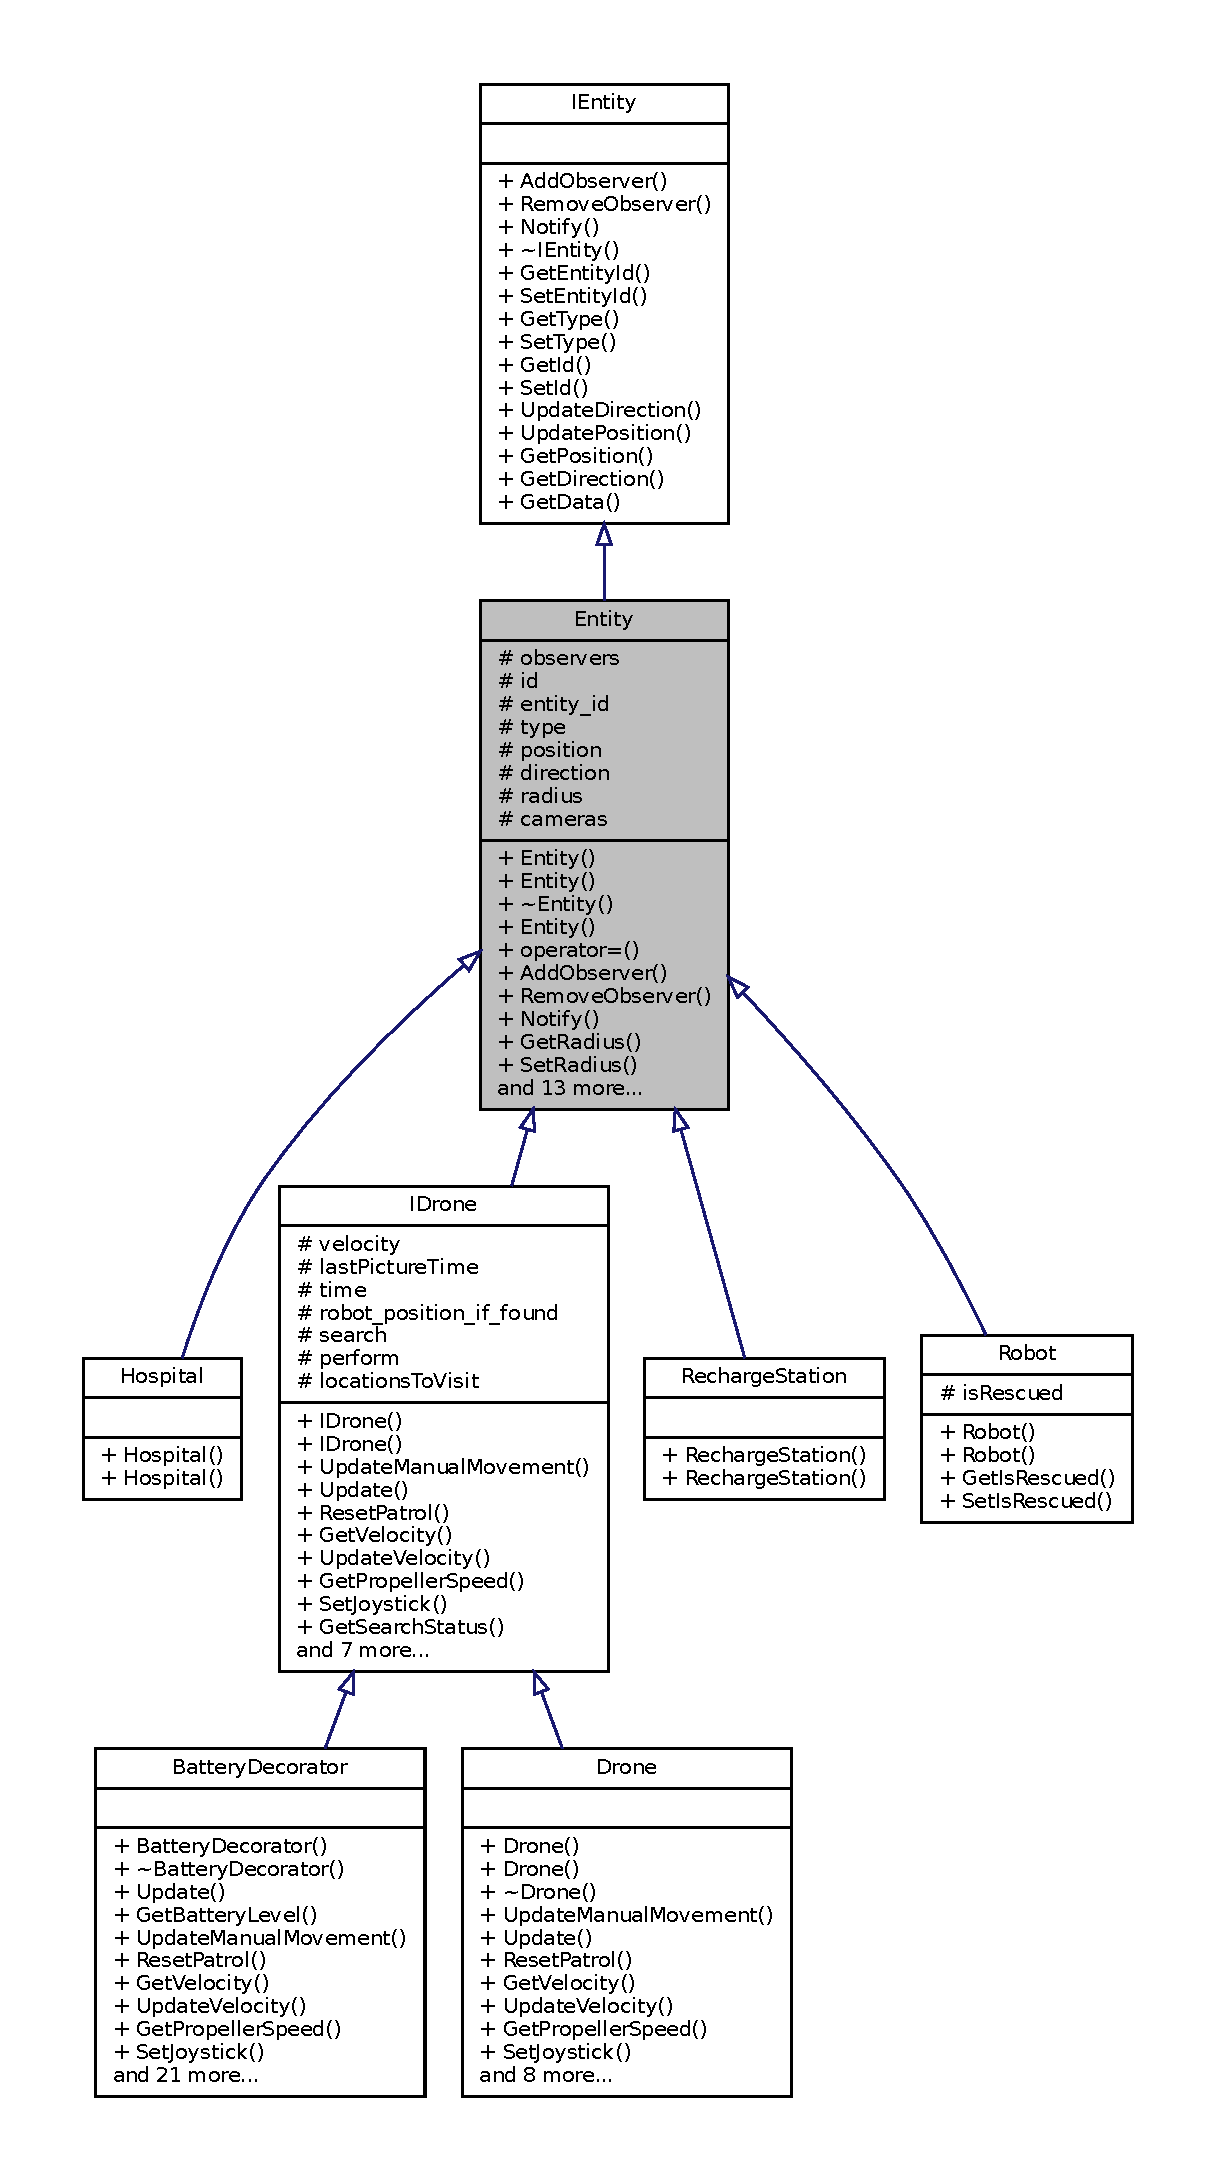
\includegraphics[height=550pt]{classEntity__inherit__graph}
\end{center}
\end{figure}


Collaboration diagram for Entity\+:\nopagebreak
\begin{figure}[H]
\begin{center}
\leavevmode
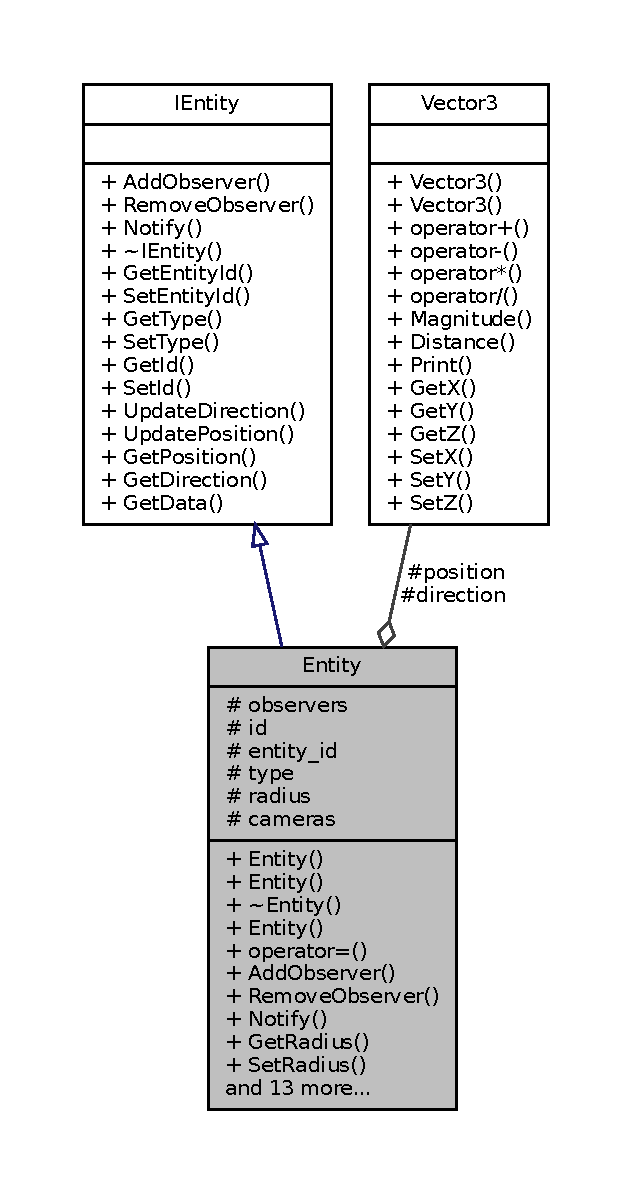
\includegraphics[height=550pt]{classEntity__coll__graph}
\end{center}
\end{figure}
\subsection*{Public Member Functions}
\begin{DoxyCompactItemize}
\item 
\mbox{\Hypertarget{classEntity_a980f368aa07ce358583982821533a54a}\label{classEntity_a980f368aa07ce358583982821533a54a}} 
\hyperlink{classEntity_a980f368aa07ce358583982821533a54a}{Entity} ()
\begin{DoxyCompactList}\small\item\em Default constructor accepting no parameters. \end{DoxyCompactList}\item 
\hyperlink{classEntity_adce4e08d76d3bfcb9703d29e7e03c145}{Entity} (picojson\+::object \&object)
\begin{DoxyCompactList}\small\item\em Constructor. \end{DoxyCompactList}\item 
\mbox{\Hypertarget{classEntity_a588098978eea6a3486b7361605ff3f0f}\label{classEntity_a588098978eea6a3486b7361605ff3f0f}} 
virtual \hyperlink{classEntity_a588098978eea6a3486b7361605ff3f0f}{$\sim$\+Entity} ()
\begin{DoxyCompactList}\small\item\em A destructor that removes/deletes all observers of the entity. \end{DoxyCompactList}\item 
\hyperlink{classEntity_ad172cbc40deff00a36d76ab8dcf9a3c2}{Entity} (const \hyperlink{classEntity}{Entity} \&object\+To\+Copy)
\begin{DoxyCompactList}\small\item\em A copy constructor that allows to copy/duplicate any \hyperlink{classEntity}{Entity}. \end{DoxyCompactList}\item 
void \hyperlink{classEntity_abc90e1d87db431ddbabc81776d8bfb04}{operator=} (const \hyperlink{classEntity}{Entity} \&object\+To\+Copy)
\begin{DoxyCompactList}\small\item\em Performs a deep copy of the \hyperlink{classEntity}{Entity} object passed in. \end{DoxyCompactList}\item 
void \hyperlink{classEntity_a13e0fdabb9f5ae73ecd4d7bf7834a3a9}{Add\+Observer} (\hyperlink{classIObserver}{I\+Observer} $\ast$new\+\_\+observer)
\begin{DoxyCompactList}\small\item\em Function that will add an observer to the entity. \end{DoxyCompactList}\item 
void \hyperlink{classEntity_a8e6bb1a529eaa32782d83824861ff29f}{Remove\+Observer} (\hyperlink{classIObserver}{I\+Observer} $\ast$observer\+\_\+to\+\_\+remove)
\begin{DoxyCompactList}\small\item\em Function that will remove an observer from the entity. \end{DoxyCompactList}\item 
void \hyperlink{classEntity_a9e180b76d5dfa6652edcffaf0aea5ec0}{Notify} (picojson\+::object \&notification)
\begin{DoxyCompactList}\small\item\em Function that will send a message to the observers of that entity so message gets notified to the UI. \end{DoxyCompactList}\item 
double \hyperlink{classEntity_a01b41a1294ffea6e11a897c633a14ef4}{Get\+Radius} ()
\begin{DoxyCompactList}\small\item\em This will return a double which represents radius of entity (for collision) \end{DoxyCompactList}\item 
void \hyperlink{classEntity_acf8bd6d266b147e86248c1ce5d925665}{Set\+Radius} (int r)
\begin{DoxyCompactList}\small\item\em This will set a double which represents radius of entity (for collision) \end{DoxyCompactList}\item 
int \hyperlink{classEntity_a0040a9ca2da893a4eccec20f542220a9}{Get\+Id} ()
\begin{DoxyCompactList}\small\item\em This will return an integer that represents the command in which the object was created. \end{DoxyCompactList}\item 
void \hyperlink{classEntity_ac806fc870b7d2419fbd207cf6ca4dd2e}{Set\+Id} (int id2)
\begin{DoxyCompactList}\small\item\em This will set the command \# in which the object was created. \end{DoxyCompactList}\item 
int \hyperlink{classEntity_afd77b9faebc188849705d91c239d193c}{Get\+Entity\+Id} ()
\begin{DoxyCompactList}\small\item\em This will return the \hyperlink{classEntity}{Entity} Id, meaning the type of object (0 represents a drone) \end{DoxyCompactList}\item 
void \hyperlink{classEntity_a2cc57041bbb23a4acdf1b2afe1756ac7}{Set\+Entity\+Id} (int id2)
\begin{DoxyCompactList}\small\item\em This will set the \hyperlink{classEntity}{Entity} Id, meaning the type of object (0 represents a drone) \end{DoxyCompactList}\item 
std\+::string \hyperlink{classEntity_a05d8f23908e47ad19e762754461c62e6}{Get\+Type} ()
\begin{DoxyCompactList}\small\item\em This will return a string representing object type \char`\"{}drone\char`\"{}, \char`\"{}hospital\char`\"{}... \end{DoxyCompactList}\item 
void \hyperlink{classEntity_a8d956360ddbff29834d22855a785fe6c}{Set\+Type} (std\+::string \&name)
\begin{DoxyCompactList}\small\item\em This will set the object type \char`\"{}drone\char`\"{}, \char`\"{}hospital\char`\"{}... \end{DoxyCompactList}\item 
void \hyperlink{classEntity_a6ae8474b6eb3684f3977dcb5406a3d11}{Update\+Direction} (const \hyperlink{classVector3}{Vector3} \&new\+Dir)
\begin{DoxyCompactList}\small\item\em Updates the direction of the entity. \end{DoxyCompactList}\item 
void \hyperlink{classEntity_ab58e8c31ba272bdd1e945130af43493f}{Update\+Position} (const \hyperlink{classVector3}{Vector3} \&new\+Dir)
\begin{DoxyCompactList}\small\item\em Updates the position of the entity. \end{DoxyCompactList}\item 
\hyperlink{classVector3}{Vector3} \hyperlink{classEntity_ac6916016f6b9b4b4d18fd988a373fddb}{Get\+Position} () const
\begin{DoxyCompactList}\small\item\em getter for entity position \end{DoxyCompactList}\item 
\hyperlink{classVector3}{Vector3} \hyperlink{classEntity_aae3890ab5d3d17ef4f805e735890f077}{Get\+Direction} () const
\begin{DoxyCompactList}\small\item\em getter for entity direction \end{DoxyCompactList}\item 
virtual void \hyperlink{classEntity_a9f3c739a3ef623a9febc7801270ba719}{Add\+Camera} (\hyperlink{classCamera}{Camera} $\ast$new\+\_\+camera)
\begin{DoxyCompactList}\small\item\em Function that will add a camera to the vector of cameras of the entity. \end{DoxyCompactList}\item 
virtual \hyperlink{classCamera}{Camera} $\ast$ \hyperlink{classEntity_ae09d3e79d0d14c2990b1da52d2268399}{Get\+Camera} (int idx)
\begin{DoxyCompactList}\small\item\em Get the idx camera from the cameras of the entity. \end{DoxyCompactList}\item 
std\+::string \hyperlink{classEntity_a25fcdac45c906ba995f427ce6facab96}{Get\+Data} (float dt)
\begin{DoxyCompactList}\small\item\em A method to get the pertinent data of an \hyperlink{classEntity}{Entity} to be written to C\+SV file. \end{DoxyCompactList}\end{DoxyCompactItemize}
\subsection*{Protected Attributes}
\begin{DoxyCompactItemize}
\item 
\mbox{\Hypertarget{classEntity_a6e98ade5dc4d06116b35b3447afbf75b}\label{classEntity_a6e98ade5dc4d06116b35b3447afbf75b}} 
std\+::vector$<$ \hyperlink{classIObserver}{I\+Observer} $\ast$ $>$ \hyperlink{classEntity_a6e98ade5dc4d06116b35b3447afbf75b}{observers}
\begin{DoxyCompactList}\small\item\em A vector of observer pointer objects that need to be notify if this entity changes states. \end{DoxyCompactList}\item 
\mbox{\Hypertarget{classEntity_aa4425a59c337b4d3b71c217ccaf511bc}\label{classEntity_aa4425a59c337b4d3b71c217ccaf511bc}} 
int \hyperlink{classEntity_aa4425a59c337b4d3b71c217ccaf511bc}{id}
\begin{DoxyCompactList}\small\item\em int representing command number when entity was created \end{DoxyCompactList}\item 
\mbox{\Hypertarget{classEntity_a3aa2fdf81f48766096b7b92c9972b13a}\label{classEntity_a3aa2fdf81f48766096b7b92c9972b13a}} 
int \hyperlink{classEntity_a3aa2fdf81f48766096b7b92c9972b13a}{entity\+\_\+id}
\begin{DoxyCompactList}\small\item\em int representing type of object (0 represents a drone) \end{DoxyCompactList}\item 
\mbox{\Hypertarget{classEntity_a298a9ebf2474bb00874b5ff6a0d637ef}\label{classEntity_a298a9ebf2474bb00874b5ff6a0d637ef}} 
std\+::string \hyperlink{classEntity_a298a9ebf2474bb00874b5ff6a0d637ef}{type}
\begin{DoxyCompactList}\small\item\em string representing object type \char`\"{}drone\char`\"{}, \char`\"{}hospital\char`\"{}... \end{DoxyCompactList}\item 
\mbox{\Hypertarget{classEntity_a09590883f0fae6e8e28751ccae8b4e93}\label{classEntity_a09590883f0fae6e8e28751ccae8b4e93}} 
\hyperlink{classVector3}{Vector3} \hyperlink{classEntity_a09590883f0fae6e8e28751ccae8b4e93}{position}
\begin{DoxyCompactList}\small\item\em A vector representing the position of the \hyperlink{classEntity}{Entity}. \end{DoxyCompactList}\item 
\mbox{\Hypertarget{classEntity_a0cbd80b9c5246037b94addee1730c41d}\label{classEntity_a0cbd80b9c5246037b94addee1730c41d}} 
\hyperlink{classVector3}{Vector3} \hyperlink{classEntity_a0cbd80b9c5246037b94addee1730c41d}{direction}
\begin{DoxyCompactList}\small\item\em A vector representing the direction of the \hyperlink{classEntity}{Entity}. \end{DoxyCompactList}\item 
\mbox{\Hypertarget{classEntity_a610ded8f251ca7e837de4497821667e5}\label{classEntity_a610ded8f251ca7e837de4497821667e5}} 
double \hyperlink{classEntity_a610ded8f251ca7e837de4497821667e5}{radius}
\begin{DoxyCompactList}\small\item\em A double representing the radius of the \hyperlink{classEntity}{Entity}. \end{DoxyCompactList}\item 
\mbox{\Hypertarget{classEntity_a1745d1d05834aab29e1591a3a0b1877d}\label{classEntity_a1745d1d05834aab29e1591a3a0b1877d}} 
std\+::vector$<$ \hyperlink{classCamera}{Camera} $\ast$ $>$ \hyperlink{classEntity_a1745d1d05834aab29e1591a3a0b1877d}{cameras}
\begin{DoxyCompactList}\small\item\em A vector of pointers to instances of the \hyperlink{classCamera}{Camera} class representing the cameras that the \hyperlink{classEntity}{Entity} can use. \end{DoxyCompactList}\end{DoxyCompactItemize}


\subsection{Constructor \& Destructor Documentation}
\mbox{\Hypertarget{classEntity_adce4e08d76d3bfcb9703d29e7e03c145}\label{classEntity_adce4e08d76d3bfcb9703d29e7e03c145}} 
\index{Entity@{Entity}!Entity@{Entity}}
\index{Entity@{Entity}!Entity@{Entity}}
\subsubsection{\texorpdfstring{Entity()}{Entity()}\hspace{0.1cm}{\footnotesize\ttfamily [1/2]}}
{\footnotesize\ttfamily Entity\+::\+Entity (\begin{DoxyParamCaption}\item[{picojson\+::object \&}]{object }\end{DoxyParamCaption})\hspace{0.3cm}{\ttfamily [inline]}}



Constructor. 


\begin{DoxyParams}[1]{Parameters}
\mbox{\tt in}  & {\em object} & picson object Object that we want to retrive info from \\
\hline
\end{DoxyParams}
\mbox{\Hypertarget{classEntity_ad172cbc40deff00a36d76ab8dcf9a3c2}\label{classEntity_ad172cbc40deff00a36d76ab8dcf9a3c2}} 
\index{Entity@{Entity}!Entity@{Entity}}
\index{Entity@{Entity}!Entity@{Entity}}
\subsubsection{\texorpdfstring{Entity()}{Entity()}\hspace{0.1cm}{\footnotesize\ttfamily [2/2]}}
{\footnotesize\ttfamily Entity\+::\+Entity (\begin{DoxyParamCaption}\item[{const \hyperlink{classEntity}{Entity} \&}]{object\+To\+Copy }\end{DoxyParamCaption})\hspace{0.3cm}{\ttfamily [inline]}}



A copy constructor that allows to copy/duplicate any \hyperlink{classEntity}{Entity}. 


\begin{DoxyParams}[1]{Parameters}
\mbox{\tt in}  & {\em object\+To\+Copy} & The \hyperlink{classEntity}{Entity} object to make a deep copy from. \\
\hline
\end{DoxyParams}


\subsection{Member Function Documentation}
\mbox{\Hypertarget{classEntity_a9f3c739a3ef623a9febc7801270ba719}\label{classEntity_a9f3c739a3ef623a9febc7801270ba719}} 
\index{Entity@{Entity}!Add\+Camera@{Add\+Camera}}
\index{Add\+Camera@{Add\+Camera}!Entity@{Entity}}
\subsubsection{\texorpdfstring{Add\+Camera()}{AddCamera()}}
{\footnotesize\ttfamily void Entity\+::\+Add\+Camera (\begin{DoxyParamCaption}\item[{\hyperlink{classCamera}{Camera} $\ast$}]{new\+\_\+camera }\end{DoxyParamCaption})\hspace{0.3cm}{\ttfamily [virtual]}}



Function that will add a camera to the vector of cameras of the entity. 


\begin{DoxyParams}[1]{Parameters}
\mbox{\tt in}  & {\em new\+\_\+camera} & New camera object to be added to the vector of cameras of the entity \\
\hline
\end{DoxyParams}


Reimplemented in \hyperlink{classBatteryDecorator_a25470bba4af4e6c112a858584a38fcdd}{Battery\+Decorator}.

\mbox{\Hypertarget{classEntity_a13e0fdabb9f5ae73ecd4d7bf7834a3a9}\label{classEntity_a13e0fdabb9f5ae73ecd4d7bf7834a3a9}} 
\index{Entity@{Entity}!Add\+Observer@{Add\+Observer}}
\index{Add\+Observer@{Add\+Observer}!Entity@{Entity}}
\subsubsection{\texorpdfstring{Add\+Observer()}{AddObserver()}}
{\footnotesize\ttfamily void Entity\+::\+Add\+Observer (\begin{DoxyParamCaption}\item[{\hyperlink{classIObserver}{I\+Observer} $\ast$}]{new\+\_\+observer }\end{DoxyParamCaption})\hspace{0.3cm}{\ttfamily [virtual]}}



Function that will add an observer to the entity. 


\begin{DoxyParams}[1]{Parameters}
\mbox{\tt in}  & {\em new\+\_\+observer} & New observer to be added that will receive notifications of the entities state changes. \\
\hline
\end{DoxyParams}


Implements \hyperlink{classIEntity_a0d682e3663a78b6b5fd3df8cd51aa321}{I\+Entity}.

\mbox{\Hypertarget{classEntity_ae09d3e79d0d14c2990b1da52d2268399}\label{classEntity_ae09d3e79d0d14c2990b1da52d2268399}} 
\index{Entity@{Entity}!Get\+Camera@{Get\+Camera}}
\index{Get\+Camera@{Get\+Camera}!Entity@{Entity}}
\subsubsection{\texorpdfstring{Get\+Camera()}{GetCamera()}}
{\footnotesize\ttfamily \hyperlink{classCamera}{Camera} $\ast$ Entity\+::\+Get\+Camera (\begin{DoxyParamCaption}\item[{int}]{idx }\end{DoxyParamCaption})\hspace{0.3cm}{\ttfamily [virtual]}}



Get the idx camera from the cameras of the entity. 


\begin{DoxyParams}[1]{Parameters}
\mbox{\tt in}  & {\em idx} & integer representing the camera you want to get\\
\hline
\end{DoxyParams}
\begin{DoxyReturn}{Returns}
\hyperlink{classCamera}{Camera} object pointer 
\end{DoxyReturn}


Reimplemented in \hyperlink{classBatteryDecorator_ad65baa2cd098b990a49bdff7c0fde62c}{Battery\+Decorator}.

\mbox{\Hypertarget{classEntity_a25fcdac45c906ba995f427ce6facab96}\label{classEntity_a25fcdac45c906ba995f427ce6facab96}} 
\index{Entity@{Entity}!Get\+Data@{Get\+Data}}
\index{Get\+Data@{Get\+Data}!Entity@{Entity}}
\subsubsection{\texorpdfstring{Get\+Data()}{GetData()}}
{\footnotesize\ttfamily std\+::string Entity\+::\+Get\+Data (\begin{DoxyParamCaption}\item[{float}]{dt }\end{DoxyParamCaption})\hspace{0.3cm}{\ttfamily [virtual]}}



A method to get the pertinent data of an \hyperlink{classEntity}{Entity} to be written to C\+SV file. 


\begin{DoxyParams}[1]{Parameters}
\mbox{\tt in}  & {\em dt} & A float representing the change in time since the last update\\
\hline
\end{DoxyParams}
\begin{DoxyReturn}{Returns}
String Returns a string containing the comma separated data to be written to a C\+SV file. 
\end{DoxyReturn}


Implements \hyperlink{classIEntity_a4d9355e68c6be349f57dc67fc1c036ba}{I\+Entity}.

\mbox{\Hypertarget{classEntity_aae3890ab5d3d17ef4f805e735890f077}\label{classEntity_aae3890ab5d3d17ef4f805e735890f077}} 
\index{Entity@{Entity}!Get\+Direction@{Get\+Direction}}
\index{Get\+Direction@{Get\+Direction}!Entity@{Entity}}
\subsubsection{\texorpdfstring{Get\+Direction()}{GetDirection()}}
{\footnotesize\ttfamily \hyperlink{classVector3}{Vector3} Entity\+::\+Get\+Direction (\begin{DoxyParamCaption}{ }\end{DoxyParamCaption}) const\hspace{0.3cm}{\ttfamily [virtual]}}



getter for entity direction 

\begin{DoxyReturn}{Returns}
\hyperlink{classVector3}{Vector3} object representing the entity direction 
\end{DoxyReturn}


Implements \hyperlink{classIEntity_aa99a8fef8b22195a5113c38ef51f086d}{I\+Entity}.

\mbox{\Hypertarget{classEntity_afd77b9faebc188849705d91c239d193c}\label{classEntity_afd77b9faebc188849705d91c239d193c}} 
\index{Entity@{Entity}!Get\+Entity\+Id@{Get\+Entity\+Id}}
\index{Get\+Entity\+Id@{Get\+Entity\+Id}!Entity@{Entity}}
\subsubsection{\texorpdfstring{Get\+Entity\+Id()}{GetEntityId()}}
{\footnotesize\ttfamily int Entity\+::\+Get\+Entity\+Id (\begin{DoxyParamCaption}{ }\end{DoxyParamCaption})\hspace{0.3cm}{\ttfamily [virtual]}}



This will return the \hyperlink{classEntity}{Entity} Id, meaning the type of object (0 represents a drone) 

\begin{DoxyReturn}{Returns}
integer representing the type of object of the entity 
\end{DoxyReturn}


Implements \hyperlink{classIEntity_a4359ee47413fa0b2940b3b0336e13861}{I\+Entity}.

\mbox{\Hypertarget{classEntity_a0040a9ca2da893a4eccec20f542220a9}\label{classEntity_a0040a9ca2da893a4eccec20f542220a9}} 
\index{Entity@{Entity}!Get\+Id@{Get\+Id}}
\index{Get\+Id@{Get\+Id}!Entity@{Entity}}
\subsubsection{\texorpdfstring{Get\+Id()}{GetId()}}
{\footnotesize\ttfamily int Entity\+::\+Get\+Id (\begin{DoxyParamCaption}{ }\end{DoxyParamCaption})\hspace{0.3cm}{\ttfamily [virtual]}}



This will return an integer that represents the command in which the object was created. 

\begin{DoxyReturn}{Returns}
id representing the command number 
\end{DoxyReturn}


Implements \hyperlink{classIEntity_ac3d60cc2fab1ccb61c1be92373e636d9}{I\+Entity}.

\mbox{\Hypertarget{classEntity_ac6916016f6b9b4b4d18fd988a373fddb}\label{classEntity_ac6916016f6b9b4b4d18fd988a373fddb}} 
\index{Entity@{Entity}!Get\+Position@{Get\+Position}}
\index{Get\+Position@{Get\+Position}!Entity@{Entity}}
\subsubsection{\texorpdfstring{Get\+Position()}{GetPosition()}}
{\footnotesize\ttfamily \hyperlink{classVector3}{Vector3} Entity\+::\+Get\+Position (\begin{DoxyParamCaption}{ }\end{DoxyParamCaption}) const\hspace{0.3cm}{\ttfamily [virtual]}}



getter for entity position 

\begin{DoxyReturn}{Returns}
\hyperlink{classVector3}{Vector3} object representing the entity position 
\end{DoxyReturn}


Implements \hyperlink{classIEntity_a9bc32587aab91761fc0e718612498199}{I\+Entity}.

\mbox{\Hypertarget{classEntity_a01b41a1294ffea6e11a897c633a14ef4}\label{classEntity_a01b41a1294ffea6e11a897c633a14ef4}} 
\index{Entity@{Entity}!Get\+Radius@{Get\+Radius}}
\index{Get\+Radius@{Get\+Radius}!Entity@{Entity}}
\subsubsection{\texorpdfstring{Get\+Radius()}{GetRadius()}}
{\footnotesize\ttfamily double Entity\+::\+Get\+Radius (\begin{DoxyParamCaption}{ }\end{DoxyParamCaption})}



This will return a double which represents radius of entity (for collision) 

\begin{DoxyReturn}{Returns}
radius of the entity as a double 
\end{DoxyReturn}
\mbox{\Hypertarget{classEntity_a05d8f23908e47ad19e762754461c62e6}\label{classEntity_a05d8f23908e47ad19e762754461c62e6}} 
\index{Entity@{Entity}!Get\+Type@{Get\+Type}}
\index{Get\+Type@{Get\+Type}!Entity@{Entity}}
\subsubsection{\texorpdfstring{Get\+Type()}{GetType()}}
{\footnotesize\ttfamily std\+::string Entity\+::\+Get\+Type (\begin{DoxyParamCaption}{ }\end{DoxyParamCaption})\hspace{0.3cm}{\ttfamily [virtual]}}



This will return a string representing object type \char`\"{}drone\char`\"{}, \char`\"{}hospital\char`\"{}... 

\begin{DoxyReturn}{Returns}
string representing the type of object of the entity 
\end{DoxyReturn}


Implements \hyperlink{classIEntity_ac494bb9712d5a03495a1a95afdbd7153}{I\+Entity}.

\mbox{\Hypertarget{classEntity_a9e180b76d5dfa6652edcffaf0aea5ec0}\label{classEntity_a9e180b76d5dfa6652edcffaf0aea5ec0}} 
\index{Entity@{Entity}!Notify@{Notify}}
\index{Notify@{Notify}!Entity@{Entity}}
\subsubsection{\texorpdfstring{Notify()}{Notify()}}
{\footnotesize\ttfamily void Entity\+::\+Notify (\begin{DoxyParamCaption}\item[{picojson\+::object \&}]{notification }\end{DoxyParamCaption})\hspace{0.3cm}{\ttfamily [virtual]}}



Function that will send a message to the observers of that entity so message gets notified to the UI. 


\begin{DoxyParams}[1]{Parameters}
\mbox{\tt in}  & {\em notification} & message specifying the entity´s state change \\
\hline
\end{DoxyParams}


Implements \hyperlink{classIEntity_acd19cac6fe0e65495f80d1962320e0c3}{I\+Entity}.

\mbox{\Hypertarget{classEntity_abc90e1d87db431ddbabc81776d8bfb04}\label{classEntity_abc90e1d87db431ddbabc81776d8bfb04}} 
\index{Entity@{Entity}!operator=@{operator=}}
\index{operator=@{operator=}!Entity@{Entity}}
\subsubsection{\texorpdfstring{operator=()}{operator=()}}
{\footnotesize\ttfamily void Entity\+::operator= (\begin{DoxyParamCaption}\item[{const \hyperlink{classEntity}{Entity} \&}]{object\+To\+Copy }\end{DoxyParamCaption})}



Performs a deep copy of the \hyperlink{classEntity}{Entity} object passed in. 


\begin{DoxyParams}[1]{Parameters}
\mbox{\tt in}  & {\em object\+To\+Copy} & The \hyperlink{classEntity}{Entity} object to copy from. \\
\hline
\end{DoxyParams}
\mbox{\Hypertarget{classEntity_a8e6bb1a529eaa32782d83824861ff29f}\label{classEntity_a8e6bb1a529eaa32782d83824861ff29f}} 
\index{Entity@{Entity}!Remove\+Observer@{Remove\+Observer}}
\index{Remove\+Observer@{Remove\+Observer}!Entity@{Entity}}
\subsubsection{\texorpdfstring{Remove\+Observer()}{RemoveObserver()}}
{\footnotesize\ttfamily void Entity\+::\+Remove\+Observer (\begin{DoxyParamCaption}\item[{\hyperlink{classIObserver}{I\+Observer} $\ast$}]{observer\+\_\+to\+\_\+remove }\end{DoxyParamCaption})\hspace{0.3cm}{\ttfamily [virtual]}}



Function that will remove an observer from the entity. 


\begin{DoxyParams}[1]{Parameters}
\mbox{\tt in}  & {\em observer\+\_\+to\+\_\+remove} & observer to be removed if present in the entity entities state changes. \\
\hline
\end{DoxyParams}


Implements \hyperlink{classIEntity_a651f1ca9f1e494af74e3f580b1c118d6}{I\+Entity}.

\mbox{\Hypertarget{classEntity_a2cc57041bbb23a4acdf1b2afe1756ac7}\label{classEntity_a2cc57041bbb23a4acdf1b2afe1756ac7}} 
\index{Entity@{Entity}!Set\+Entity\+Id@{Set\+Entity\+Id}}
\index{Set\+Entity\+Id@{Set\+Entity\+Id}!Entity@{Entity}}
\subsubsection{\texorpdfstring{Set\+Entity\+Id()}{SetEntityId()}}
{\footnotesize\ttfamily void Entity\+::\+Set\+Entity\+Id (\begin{DoxyParamCaption}\item[{int}]{id2 }\end{DoxyParamCaption})\hspace{0.3cm}{\ttfamily [virtual]}}



This will set the \hyperlink{classEntity}{Entity} Id, meaning the type of object (0 represents a drone) 


\begin{DoxyParams}[1]{Parameters}
\mbox{\tt in}  & {\em id2} & integer representing the type of object of the entity \\
\hline
\end{DoxyParams}


Implements \hyperlink{classIEntity_a3a830862181cb0548d2aca83d908263e}{I\+Entity}.

\mbox{\Hypertarget{classEntity_ac806fc870b7d2419fbd207cf6ca4dd2e}\label{classEntity_ac806fc870b7d2419fbd207cf6ca4dd2e}} 
\index{Entity@{Entity}!Set\+Id@{Set\+Id}}
\index{Set\+Id@{Set\+Id}!Entity@{Entity}}
\subsubsection{\texorpdfstring{Set\+Id()}{SetId()}}
{\footnotesize\ttfamily void Entity\+::\+Set\+Id (\begin{DoxyParamCaption}\item[{int}]{id2 }\end{DoxyParamCaption})\hspace{0.3cm}{\ttfamily [virtual]}}



This will set the command \# in which the object was created. 


\begin{DoxyParams}[1]{Parameters}
\mbox{\tt in}  & {\em id2} & the command number as an integer \\
\hline
\end{DoxyParams}


Implements \hyperlink{classIEntity_a8c6af682e07f569ba2f164d214295c67}{I\+Entity}.

\mbox{\Hypertarget{classEntity_acf8bd6d266b147e86248c1ce5d925665}\label{classEntity_acf8bd6d266b147e86248c1ce5d925665}} 
\index{Entity@{Entity}!Set\+Radius@{Set\+Radius}}
\index{Set\+Radius@{Set\+Radius}!Entity@{Entity}}
\subsubsection{\texorpdfstring{Set\+Radius()}{SetRadius()}}
{\footnotesize\ttfamily void Entity\+::\+Set\+Radius (\begin{DoxyParamCaption}\item[{int}]{r }\end{DoxyParamCaption})}



This will set a double which represents radius of entity (for collision) 


\begin{DoxyParams}[1]{Parameters}
\mbox{\tt in}  & {\em r} & radius of the entity as a double \\
\hline
\end{DoxyParams}
\mbox{\Hypertarget{classEntity_a8d956360ddbff29834d22855a785fe6c}\label{classEntity_a8d956360ddbff29834d22855a785fe6c}} 
\index{Entity@{Entity}!Set\+Type@{Set\+Type}}
\index{Set\+Type@{Set\+Type}!Entity@{Entity}}
\subsubsection{\texorpdfstring{Set\+Type()}{SetType()}}
{\footnotesize\ttfamily void Entity\+::\+Set\+Type (\begin{DoxyParamCaption}\item[{std\+::string \&}]{name }\end{DoxyParamCaption})\hspace{0.3cm}{\ttfamily [virtual]}}



This will set the object type \char`\"{}drone\char`\"{}, \char`\"{}hospital\char`\"{}... 


\begin{DoxyParams}[1]{Parameters}
\mbox{\tt in}  & {\em name} & string representing the type of object of the entity \\
\hline
\end{DoxyParams}


Implements \hyperlink{classIEntity_a49b3c54f94a93d4a9f96527ffb8982f5}{I\+Entity}.

\mbox{\Hypertarget{classEntity_a6ae8474b6eb3684f3977dcb5406a3d11}\label{classEntity_a6ae8474b6eb3684f3977dcb5406a3d11}} 
\index{Entity@{Entity}!Update\+Direction@{Update\+Direction}}
\index{Update\+Direction@{Update\+Direction}!Entity@{Entity}}
\subsubsection{\texorpdfstring{Update\+Direction()}{UpdateDirection()}}
{\footnotesize\ttfamily void Entity\+::\+Update\+Direction (\begin{DoxyParamCaption}\item[{const \hyperlink{classVector3}{Vector3} \&}]{new\+Dir }\end{DoxyParamCaption})\hspace{0.3cm}{\ttfamily [virtual]}}



Updates the direction of the entity. 


\begin{DoxyParams}[1]{Parameters}
\mbox{\tt in}  & {\em new\+Dir} & vector3 representing the new direction of the object \\
\hline
\end{DoxyParams}


Implements \hyperlink{classIEntity_af24054e349dcdaea31a778427a34495d}{I\+Entity}.

\mbox{\Hypertarget{classEntity_ab58e8c31ba272bdd1e945130af43493f}\label{classEntity_ab58e8c31ba272bdd1e945130af43493f}} 
\index{Entity@{Entity}!Update\+Position@{Update\+Position}}
\index{Update\+Position@{Update\+Position}!Entity@{Entity}}
\subsubsection{\texorpdfstring{Update\+Position()}{UpdatePosition()}}
{\footnotesize\ttfamily void Entity\+::\+Update\+Position (\begin{DoxyParamCaption}\item[{const \hyperlink{classVector3}{Vector3} \&}]{new\+Dir }\end{DoxyParamCaption})\hspace{0.3cm}{\ttfamily [virtual]}}



Updates the position of the entity. 


\begin{DoxyParams}[1]{Parameters}
\mbox{\tt in}  & {\em new\+Dir} & vector3 representing the new position of the object \\
\hline
\end{DoxyParams}


Implements \hyperlink{classIEntity_ad30f6845c8747534e7607ca97addbdc6}{I\+Entity}.



The documentation for this class was generated from the following files\+:\begin{DoxyCompactItemize}
\item 
/home/user/repo/project/src/\+Entity/\hyperlink{Entity_8h}{Entity.\+h}\item 
/home/user/repo/project/src/\+Entity/\hyperlink{Entity_8cc}{Entity.\+cc}\end{DoxyCompactItemize}

\hypertarget{classEntityFactory}{}\section{Entity\+Factory Class Reference}
\label{classEntityFactory}\index{Entity\+Factory@{Entity\+Factory}}


Inheritance diagram for Entity\+Factory\+:\nopagebreak
\begin{figure}[H]
\begin{center}
\leavevmode
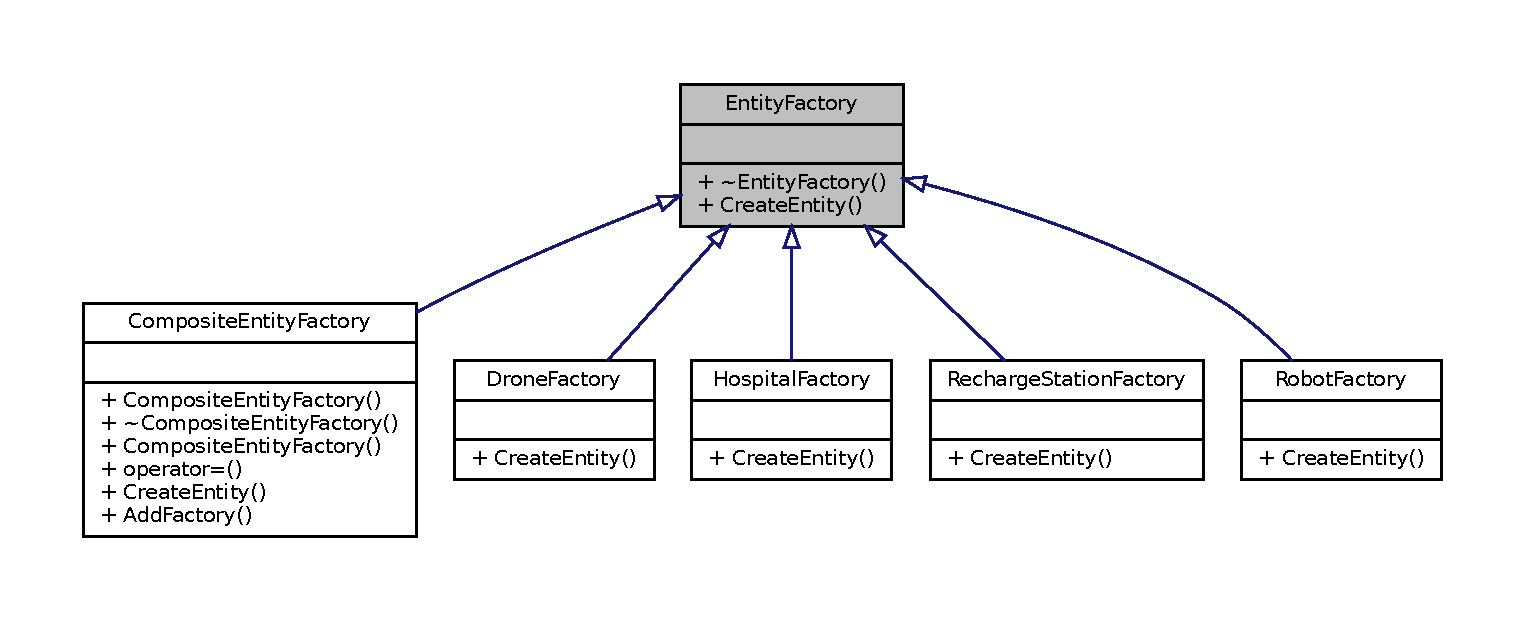
\includegraphics[width=350pt]{classEntityFactory__inherit__graph}
\end{center}
\end{figure}


Collaboration diagram for Entity\+Factory\+:\nopagebreak
\begin{figure}[H]
\begin{center}
\leavevmode
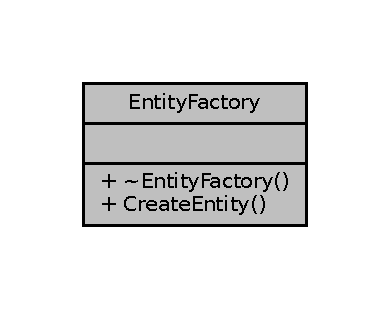
\includegraphics[width=187pt]{classEntityFactory__coll__graph}
\end{center}
\end{figure}
\subsection*{Public Member Functions}
\begin{DoxyCompactItemize}
\item 
\mbox{\Hypertarget{classEntityFactory_ae3246f06fa101178803f76582323d4ad}\label{classEntityFactory_ae3246f06fa101178803f76582323d4ad}} 
virtual \hyperlink{classEntityFactory_ae3246f06fa101178803f76582323d4ad}{$\sim$\+Entity\+Factory} ()=default
\begin{DoxyCompactList}\small\item\em virtual destructor since composite Factory needs to be called and that is a subclass \end{DoxyCompactList}\item 
virtual \hyperlink{classIEntity}{I\+Entity} $\ast$ \hyperlink{classEntityFactory_a7f579ca02f15935e6901e5c955c9726a}{Create\+Entity} (picojson\+::object \&object, \hyperlink{classICameraController}{I\+Camera\+Controller} \&camera\+Controller)=0
\begin{DoxyCompactList}\small\item\em creates an entity based on the picson object \end{DoxyCompactList}\end{DoxyCompactItemize}


\subsection{Member Function Documentation}
\mbox{\Hypertarget{classEntityFactory_a7f579ca02f15935e6901e5c955c9726a}\label{classEntityFactory_a7f579ca02f15935e6901e5c955c9726a}} 
\index{Entity\+Factory@{Entity\+Factory}!Create\+Entity@{Create\+Entity}}
\index{Create\+Entity@{Create\+Entity}!Entity\+Factory@{Entity\+Factory}}
\subsubsection{\texorpdfstring{Create\+Entity()}{CreateEntity()}}
{\footnotesize\ttfamily virtual \hyperlink{classIEntity}{I\+Entity}$\ast$ Entity\+Factory\+::\+Create\+Entity (\begin{DoxyParamCaption}\item[{picojson\+::object \&}]{object,  }\item[{\hyperlink{classICameraController}{I\+Camera\+Controller} \&}]{camera\+Controller }\end{DoxyParamCaption})\hspace{0.3cm}{\ttfamily [pure virtual]}}



creates an entity based on the picson object 


\begin{DoxyParams}[1]{Parameters}
\mbox{\tt in}  & {\em object} & json object representing the entity that needs to be created\\
\hline
\end{DoxyParams}
\begin{DoxyReturn}{Returns}
entity object or nullpointer 
\end{DoxyReturn}


Implemented in \hyperlink{classCompositeEntityFactory_a97b2f95333369f946d0f3ab2116b5f19}{Composite\+Entity\+Factory}, \hyperlink{classDroneFactory_a058b7be67ed594854ab9605236fa5c7e}{Drone\+Factory}, \hyperlink{classRechargeStationFactory_a5a870c5d317e1ec6932dc2a03d571474}{Recharge\+Station\+Factory}, \hyperlink{classRobotFactory_abcf3e19faf1d87fe2393b275b07c3549}{Robot\+Factory}, and \hyperlink{classHospitalFactory_a03bde29949e311469a3153da4e833622}{Hospital\+Factory}.



The documentation for this class was generated from the following file\+:\begin{DoxyCompactItemize}
\item 
/home/user/repo/project/src/\+Factory/\hyperlink{EntityFactory_8h}{Entity\+Factory.\+h}\end{DoxyCompactItemize}

\hypertarget{classFilter}{}\section{Filter Class Reference}
\label{classFilter}\index{Filter@{Filter}}


Abstract class that defines the virtual methods for all filter classes.  




{\ttfamily \#include $<$filter.\+h$>$}



Inheritance diagram for Filter\+:\nopagebreak
\begin{figure}[H]
\begin{center}
\leavevmode
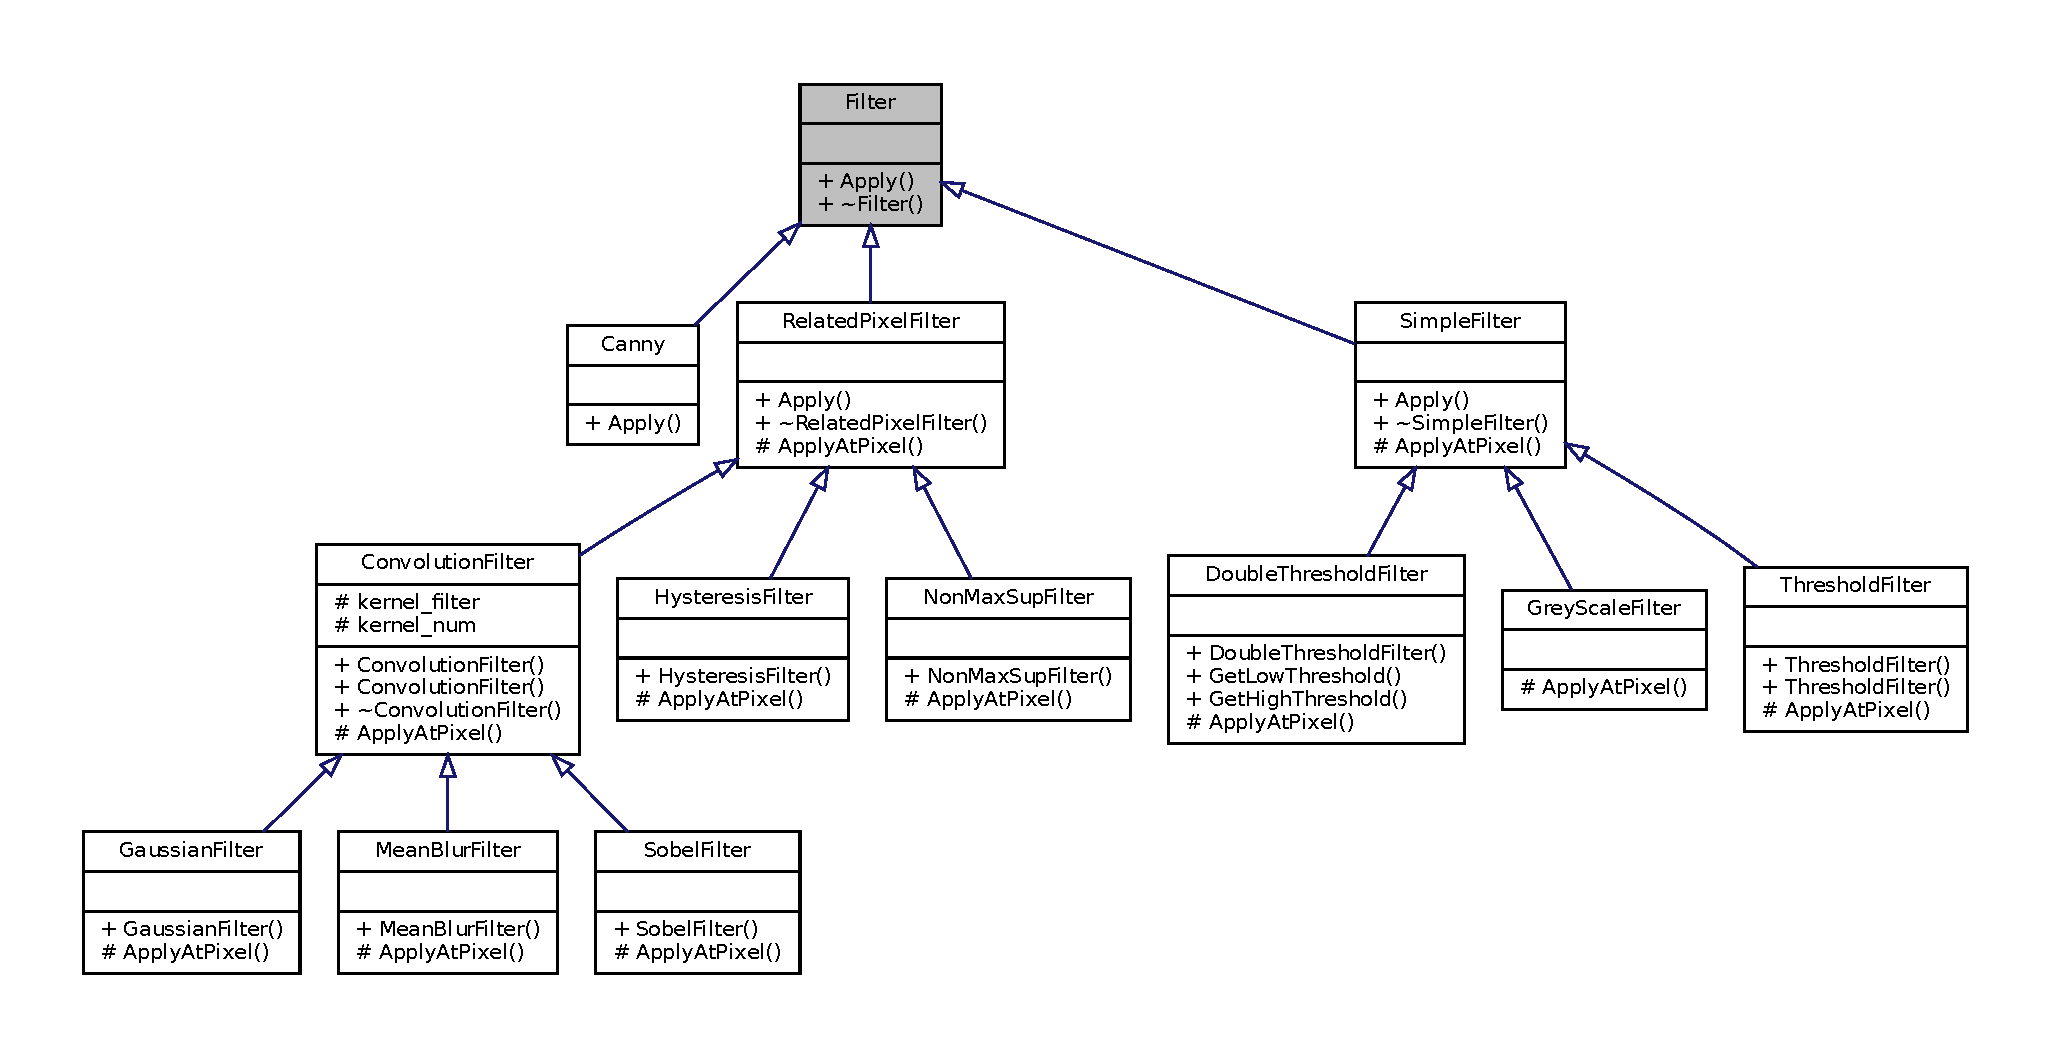
\includegraphics[width=350pt]{classFilter__inherit__graph}
\end{center}
\end{figure}


Collaboration diagram for Filter\+:\nopagebreak
\begin{figure}[H]
\begin{center}
\leavevmode
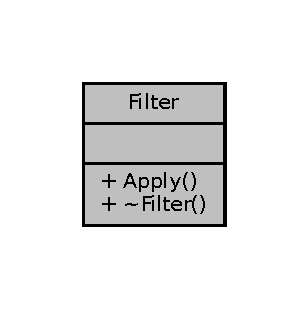
\includegraphics[width=148pt]{classFilter__coll__graph}
\end{center}
\end{figure}
\subsection*{Public Member Functions}
\begin{DoxyCompactItemize}
\item 
virtual void \hyperlink{classFilter_afab0d50af44a19a370ebe46c69b8ff4e}{Apply} (std\+::vector$<$ \hyperlink{classImage}{Image} $\ast$$>$ original, std\+::vector$<$ \hyperlink{classImage}{Image} $\ast$$>$ filtered)=0
\begin{DoxyCompactList}\small\item\em Pure virtual method for \hyperlink{classFilter}{Filter}. \end{DoxyCompactList}\item 
\mbox{\Hypertarget{classFilter_aa37dc017d133404b3a326f363ce36b8a}\label{classFilter_aa37dc017d133404b3a326f363ce36b8a}} 
virtual \hyperlink{classFilter_aa37dc017d133404b3a326f363ce36b8a}{$\sim$\+Filter} ()
\begin{DoxyCompactList}\small\item\em Virtual destructor that is needed for polymorphism since derived classes constructors need to be called. \end{DoxyCompactList}\end{DoxyCompactItemize}


\subsection{Detailed Description}
Abstract class that defines the virtual methods for all filter classes. 

\subsection{Member Function Documentation}
\mbox{\Hypertarget{classFilter_afab0d50af44a19a370ebe46c69b8ff4e}\label{classFilter_afab0d50af44a19a370ebe46c69b8ff4e}} 
\index{Filter@{Filter}!Apply@{Apply}}
\index{Apply@{Apply}!Filter@{Filter}}
\subsubsection{\texorpdfstring{Apply()}{Apply()}}
{\footnotesize\ttfamily virtual void Filter\+::\+Apply (\begin{DoxyParamCaption}\item[{std\+::vector$<$ \hyperlink{classImage}{Image} $\ast$$>$}]{original,  }\item[{std\+::vector$<$ \hyperlink{classImage}{Image} $\ast$$>$}]{filtered }\end{DoxyParamCaption})\hspace{0.3cm}{\ttfamily [pure virtual]}}



Pure virtual method for \hyperlink{classFilter}{Filter}. 


\begin{DoxyParams}[1]{Parameters}
\mbox{\tt in}  & {\em original} & A vector of input images to apply the filter on. \\
\hline
\mbox{\tt in}  & {\em filtered} & A vector of output images that contain the images with the filter applied. \\
\hline
\end{DoxyParams}


Implemented in \hyperlink{classSimpleFilter_a4400a0f97e26e84a33befd537fb4fea8}{Simple\+Filter}, \hyperlink{classCanny_aefadd0d0166f26f76d6bf2cf59dae3aa}{Canny}, and \hyperlink{classRelatedPixelFilter_a4f78d98d7f5ddc55f1e5e0f029b2bfbe}{Related\+Pixel\+Filter}.



The documentation for this class was generated from the following file\+:\begin{DoxyCompactItemize}
\item 
/home/user/repo/project/\+Image\+Processing/\hyperlink{filter_8h}{filter.\+h}\end{DoxyCompactItemize}

\hypertarget{classGaussianFilter}{}\section{Gaussian\+Filter Class Reference}
\label{classGaussianFilter}\index{Gaussian\+Filter@{Gaussian\+Filter}}


A \hyperlink{classConvolutionFilter}{Convolution\+Filter} that computes a gaussian kernel given a kernel size and sigma.  




{\ttfamily \#include $<$gaussian\+\_\+filter.\+h$>$}



Inheritance diagram for Gaussian\+Filter\+:\nopagebreak
\begin{figure}[H]
\begin{center}
\leavevmode
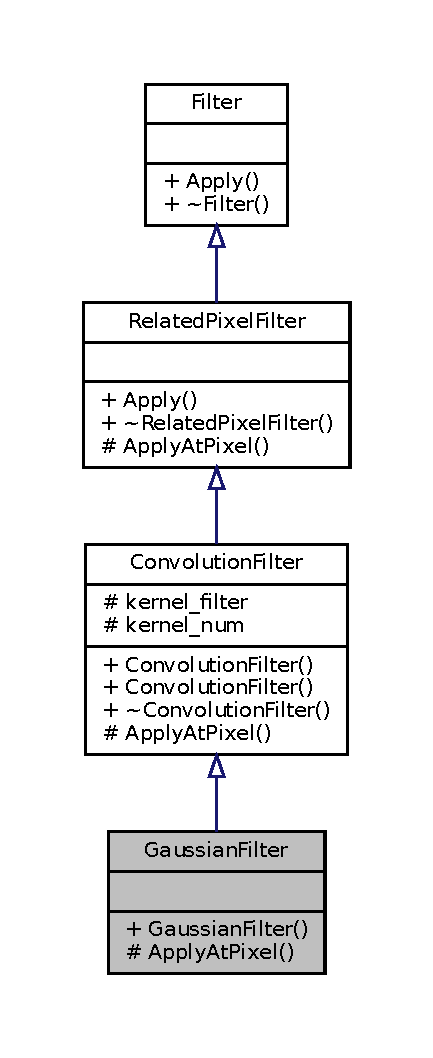
\includegraphics[width=208pt]{classGaussianFilter__inherit__graph}
\end{center}
\end{figure}


Collaboration diagram for Gaussian\+Filter\+:\nopagebreak
\begin{figure}[H]
\begin{center}
\leavevmode
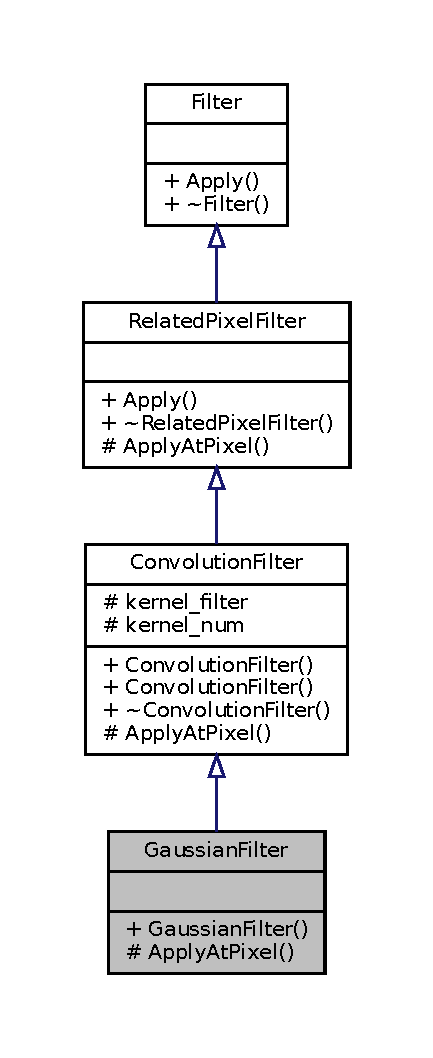
\includegraphics[width=208pt]{classGaussianFilter__coll__graph}
\end{center}
\end{figure}
\subsection*{Public Member Functions}
\begin{DoxyCompactItemize}
\item 
\mbox{\Hypertarget{classGaussianFilter_a45e674167d95fda302e9e2344f8d690c}\label{classGaussianFilter_a45e674167d95fda302e9e2344f8d690c}} 
\hyperlink{classGaussianFilter_a45e674167d95fda302e9e2344f8d690c}{Gaussian\+Filter} (int size, float sigma)
\begin{DoxyCompactList}\small\item\em Constructor that is called in parent constructor passing the 1 kernels needed for the filter, calls the Gaussian\+Kernel method to generate the kernel. \end{DoxyCompactList}\end{DoxyCompactItemize}
\subsection*{Protected Member Functions}
\begin{DoxyCompactItemize}
\item 
std\+::vector$<$ \hyperlink{classColor}{Color} $>$ \hyperlink{classGaussianFilter_af8bf2d0f68642e6232f8b73ef1bee512}{Apply\+At\+Pixel} (const std\+::vector$<$ \hyperlink{classImage}{Image} $\ast$$>$ original, int x, int y)
\begin{DoxyCompactList}\small\item\em method that applies the mean blur filter to a single pixel. \end{DoxyCompactList}\end{DoxyCompactItemize}
\subsection*{Additional Inherited Members}


\subsection{Detailed Description}
A \hyperlink{classConvolutionFilter}{Convolution\+Filter} that computes a gaussian kernel given a kernel size and sigma. 

\subsection{Member Function Documentation}
\mbox{\Hypertarget{classGaussianFilter_af8bf2d0f68642e6232f8b73ef1bee512}\label{classGaussianFilter_af8bf2d0f68642e6232f8b73ef1bee512}} 
\index{Gaussian\+Filter@{Gaussian\+Filter}!Apply\+At\+Pixel@{Apply\+At\+Pixel}}
\index{Apply\+At\+Pixel@{Apply\+At\+Pixel}!Gaussian\+Filter@{Gaussian\+Filter}}
\subsubsection{\texorpdfstring{Apply\+At\+Pixel()}{ApplyAtPixel()}}
{\footnotesize\ttfamily std\+::vector$<$ \hyperlink{classColor}{Color} $>$ Gaussian\+Filter\+::\+Apply\+At\+Pixel (\begin{DoxyParamCaption}\item[{const std\+::vector$<$ \hyperlink{classImage}{Image} $\ast$$>$}]{original,  }\item[{int}]{x,  }\item[{int}]{y }\end{DoxyParamCaption})\hspace{0.3cm}{\ttfamily [protected]}, {\ttfamily [virtual]}}



method that applies the mean blur filter to a single pixel. 


\begin{DoxyParams}[1]{Parameters}
\mbox{\tt in}  & {\em original} & A vector of input images to apply the filter over. \\
\hline
\mbox{\tt in}  & {\em x} & An integer representing the width in which the image color pixel is located, and the pixel to which the filter should be applied. \\
\hline
\mbox{\tt in}  & {\em y} & An integer representing the height in which the image color pixel is located, and the pixel to which the filter should be applied.\\
\hline
\end{DoxyParams}
\begin{DoxyReturn}{Returns}
A unique pointer array containing a \hyperlink{classColor}{Color} for each filtered image the filter should produce as an output, for the mean blur filter the vector should only contain one color object. 
\end{DoxyReturn}


Implements \hyperlink{classConvolutionFilter_abc4b4ffef2b69fc2b7164e96af6cf186}{Convolution\+Filter}.



The documentation for this class was generated from the following files\+:\begin{DoxyCompactItemize}
\item 
/home/user/repo/project/\+Image\+Processing/\hyperlink{gaussian__filter_8h}{gaussian\+\_\+filter.\+h}\item 
/home/user/repo/project/\+Image\+Processing/\hyperlink{gaussian__filter_8cc}{gaussian\+\_\+filter.\+cc}\end{DoxyCompactItemize}

\hypertarget{classGreyScaleFilter}{}\section{Grey\+Scale\+Filter Class Reference}
\label{classGreyScaleFilter}\index{Grey\+Scale\+Filter@{Grey\+Scale\+Filter}}


Greyscale filter is a \hyperlink{classSimpleFilter}{Simple\+Filter} that sets R\+GB vales for each pixel in an image to be the luminance of the pixel.  




{\ttfamily \#include $<$greyscale\+\_\+filter.\+h$>$}



Inheritance diagram for Grey\+Scale\+Filter\+:\nopagebreak
\begin{figure}[H]
\begin{center}
\leavevmode
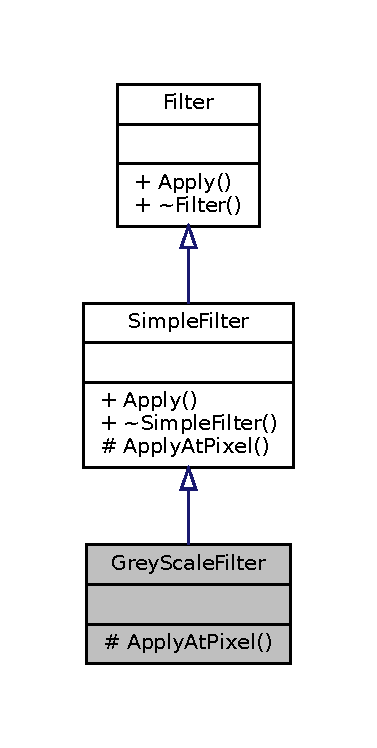
\includegraphics[width=181pt]{classGreyScaleFilter__inherit__graph}
\end{center}
\end{figure}


Collaboration diagram for Grey\+Scale\+Filter\+:\nopagebreak
\begin{figure}[H]
\begin{center}
\leavevmode
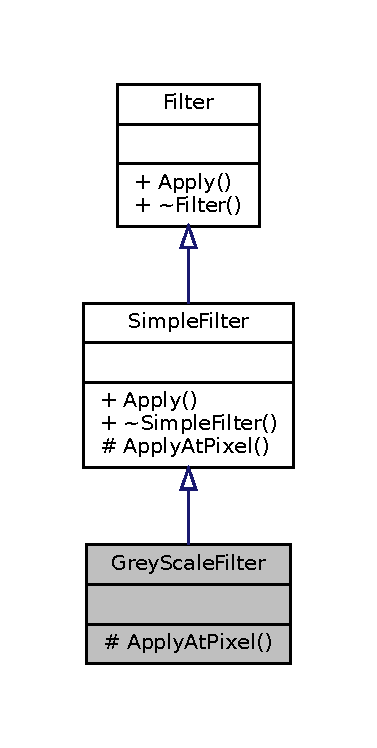
\includegraphics[width=181pt]{classGreyScaleFilter__coll__graph}
\end{center}
\end{figure}
\subsection*{Protected Member Functions}
\begin{DoxyCompactItemize}
\item 
\hyperlink{classColor}{Color} \hyperlink{classGreyScaleFilter_a4b86977b204bf2699c4d138d6d0a1116}{Apply\+At\+Pixel} (const \hyperlink{classImage}{Image} $\ast$image, const \hyperlink{classColor}{Color} \&pixel)
\begin{DoxyCompactList}\small\item\em Applies the filter to one single pixel. \end{DoxyCompactList}\end{DoxyCompactItemize}
\subsection*{Additional Inherited Members}


\subsection{Detailed Description}
Greyscale filter is a \hyperlink{classSimpleFilter}{Simple\+Filter} that sets R\+GB vales for each pixel in an image to be the luminance of the pixel. 

\subsection{Member Function Documentation}
\mbox{\Hypertarget{classGreyScaleFilter_a4b86977b204bf2699c4d138d6d0a1116}\label{classGreyScaleFilter_a4b86977b204bf2699c4d138d6d0a1116}} 
\index{Grey\+Scale\+Filter@{Grey\+Scale\+Filter}!Apply\+At\+Pixel@{Apply\+At\+Pixel}}
\index{Apply\+At\+Pixel@{Apply\+At\+Pixel}!Grey\+Scale\+Filter@{Grey\+Scale\+Filter}}
\subsubsection{\texorpdfstring{Apply\+At\+Pixel()}{ApplyAtPixel()}}
{\footnotesize\ttfamily \hyperlink{classColor}{Color} Grey\+Scale\+Filter\+::\+Apply\+At\+Pixel (\begin{DoxyParamCaption}\item[{const \hyperlink{classImage}{Image} $\ast$}]{image,  }\item[{const \hyperlink{classColor}{Color} \&}]{pixel }\end{DoxyParamCaption})\hspace{0.3cm}{\ttfamily [protected]}, {\ttfamily [virtual]}}



Applies the filter to one single pixel. 


\begin{DoxyParams}[1]{Parameters}
\mbox{\tt in}  & {\em image} & A constant pointer to an instance of the \hyperlink{classImage}{Image} class. \\
\hline
\mbox{\tt in}  & {\em pixel} & \hyperlink{classColor}{Color} object representing the pixel to apply the Gray\+Scale filter.\\
\hline
\end{DoxyParams}
\begin{DoxyReturn}{Returns}
A \hyperlink{classColor}{Color} object representing the pixel after the filter has been applied. 
\end{DoxyReturn}


Implements \hyperlink{classSimpleFilter_aa12dc75dac8932ce03a9c9a3c7964b30}{Simple\+Filter}.



The documentation for this class was generated from the following files\+:\begin{DoxyCompactItemize}
\item 
/home/user/repo/project/\+Image\+Processing/\hyperlink{greyscale__filter_8h}{greyscale\+\_\+filter.\+h}\item 
/home/user/repo/project/\+Image\+Processing/\hyperlink{greyscale__filter_8cc}{greyscale\+\_\+filter.\+cc}\end{DoxyCompactItemize}

\hypertarget{classHospital}{}\section{Hospital Class Reference}
\label{classHospital}\index{Hospital@{Hospital}}


Inheritance diagram for Hospital\+:\nopagebreak
\begin{figure}[H]
\begin{center}
\leavevmode
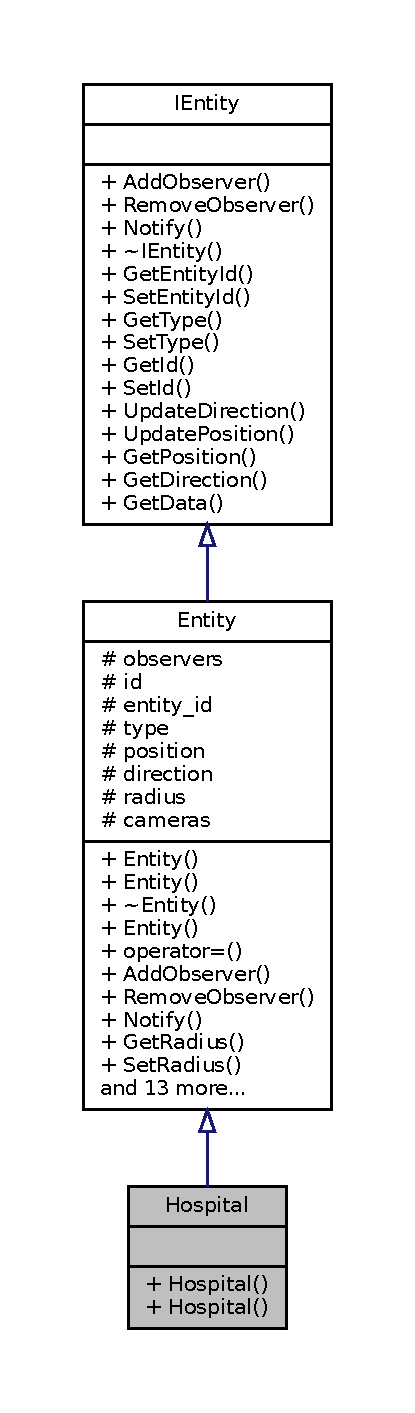
\includegraphics[height=550pt]{classHospital__inherit__graph}
\end{center}
\end{figure}


Collaboration diagram for Hospital\+:\nopagebreak
\begin{figure}[H]
\begin{center}
\leavevmode
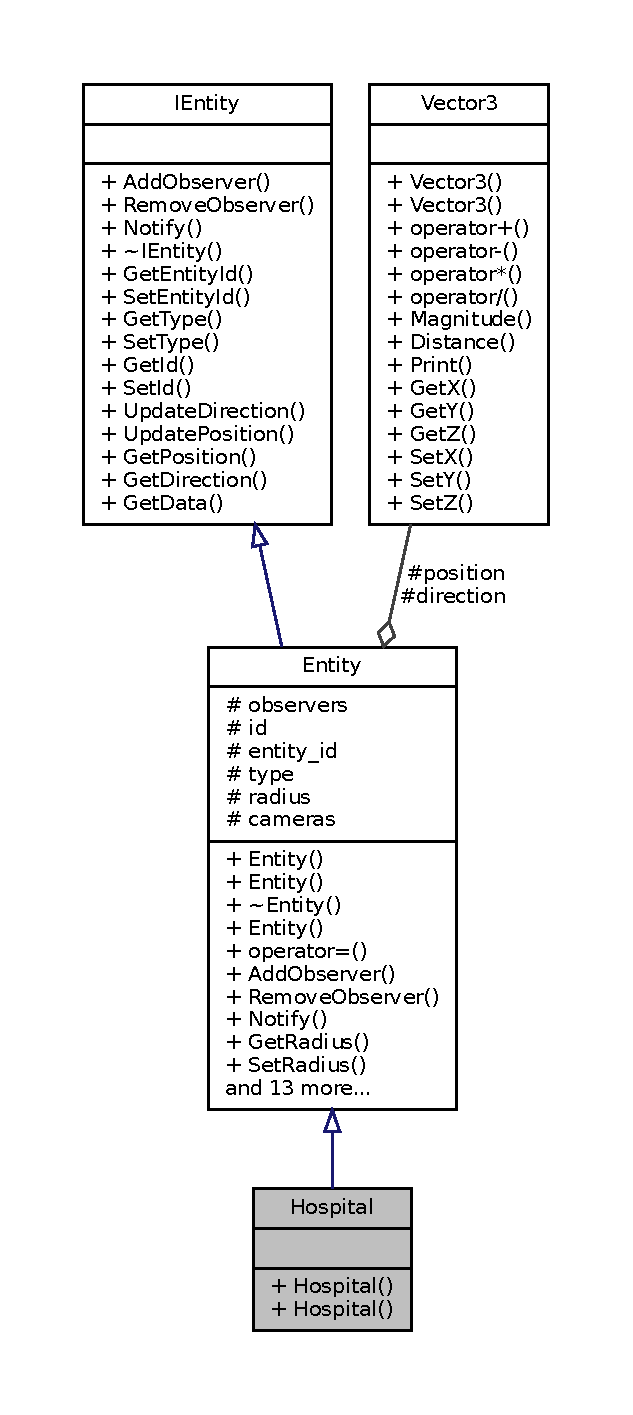
\includegraphics[height=550pt]{classHospital__coll__graph}
\end{center}
\end{figure}
\subsection*{Public Member Functions}
\begin{DoxyCompactItemize}
\item 
\mbox{\Hypertarget{classHospital_a130b3a6c6e3dd35443437e1f5144b1ac}\label{classHospital_a130b3a6c6e3dd35443437e1f5144b1ac}} 
\hyperlink{classHospital_a130b3a6c6e3dd35443437e1f5144b1ac}{Hospital} ()
\begin{DoxyCompactList}\small\item\em Default constructor accepting no parameters. \end{DoxyCompactList}\item 
\hyperlink{classHospital_aebc8b47c3d12ea7fc500981d89341e82}{Hospital} (picojson\+::object \&obj)
\begin{DoxyCompactList}\small\item\em Constructor. \end{DoxyCompactList}\end{DoxyCompactItemize}
\subsection*{Additional Inherited Members}


\subsection{Constructor \& Destructor Documentation}
\mbox{\Hypertarget{classHospital_aebc8b47c3d12ea7fc500981d89341e82}\label{classHospital_aebc8b47c3d12ea7fc500981d89341e82}} 
\index{Hospital@{Hospital}!Hospital@{Hospital}}
\index{Hospital@{Hospital}!Hospital@{Hospital}}
\subsubsection{\texorpdfstring{Hospital()}{Hospital()}}
{\footnotesize\ttfamily Hospital\+::\+Hospital (\begin{DoxyParamCaption}\item[{picojson\+::object \&}]{obj }\end{DoxyParamCaption})\hspace{0.3cm}{\ttfamily [inline]}}



Constructor. 


\begin{DoxyParams}[1]{Parameters}
\mbox{\tt in}  & {\em object} & picson object Object that we want to retrive info from \\
\hline
\end{DoxyParams}


The documentation for this class was generated from the following file\+:\begin{DoxyCompactItemize}
\item 
/home/user/repo/project/src/\+Entity/\hyperlink{Hospital_8h}{Hospital.\+h}\end{DoxyCompactItemize}

\hypertarget{classHospitalFactory}{}\section{Hospital\+Factory Class Reference}
\label{classHospitalFactory}\index{Hospital\+Factory@{Hospital\+Factory}}


Inheritance diagram for Hospital\+Factory\+:\nopagebreak
\begin{figure}[H]
\begin{center}
\leavevmode
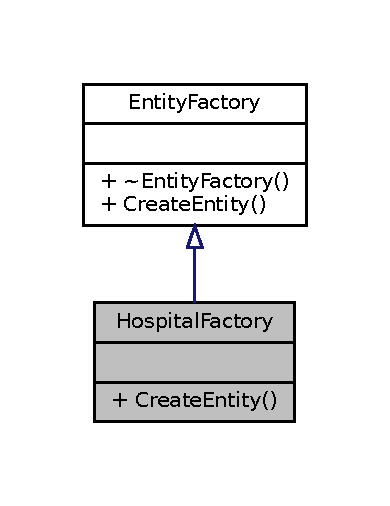
\includegraphics[width=187pt]{classHospitalFactory__inherit__graph}
\end{center}
\end{figure}


Collaboration diagram for Hospital\+Factory\+:\nopagebreak
\begin{figure}[H]
\begin{center}
\leavevmode
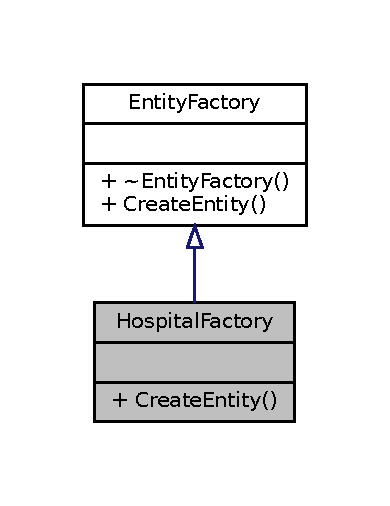
\includegraphics[width=187pt]{classHospitalFactory__coll__graph}
\end{center}
\end{figure}
\subsection*{Public Member Functions}
\begin{DoxyCompactItemize}
\item 
\hyperlink{classIEntity}{I\+Entity} $\ast$ \hyperlink{classHospitalFactory_a03bde29949e311469a3153da4e833622}{Create\+Entity} (picojson\+::object \&object, \hyperlink{classICameraController}{I\+Camera\+Controller} \&camera\+Controller)
\begin{DoxyCompactList}\small\item\em creates a hospital based on the picson object \end{DoxyCompactList}\end{DoxyCompactItemize}


\subsection{Member Function Documentation}
\mbox{\Hypertarget{classHospitalFactory_a03bde29949e311469a3153da4e833622}\label{classHospitalFactory_a03bde29949e311469a3153da4e833622}} 
\index{Hospital\+Factory@{Hospital\+Factory}!Create\+Entity@{Create\+Entity}}
\index{Create\+Entity@{Create\+Entity}!Hospital\+Factory@{Hospital\+Factory}}
\subsubsection{\texorpdfstring{Create\+Entity()}{CreateEntity()}}
{\footnotesize\ttfamily \hyperlink{classIEntity}{I\+Entity} $\ast$ Hospital\+Factory\+::\+Create\+Entity (\begin{DoxyParamCaption}\item[{picojson\+::object \&}]{object,  }\item[{\hyperlink{classICameraController}{I\+Camera\+Controller} \&}]{camera\+Controller }\end{DoxyParamCaption})\hspace{0.3cm}{\ttfamily [virtual]}}



creates a hospital based on the picson object 


\begin{DoxyParams}[1]{Parameters}
\mbox{\tt in}  & {\em object} & json object containing hospital details\\
\hline
\end{DoxyParams}
\begin{DoxyReturn}{Returns}
entity object or nullpointer 
\end{DoxyReturn}


Implements \hyperlink{classEntityFactory_a7f579ca02f15935e6901e5c955c9726a}{Entity\+Factory}.



The documentation for this class was generated from the following files\+:\begin{DoxyCompactItemize}
\item 
/home/user/repo/project/src/\+Factory/\hyperlink{HospitalFactory_8h}{Hospital\+Factory.\+h}\item 
/home/user/repo/project/src/\+Factory/\hyperlink{HospitalFactory_8cc}{Hospital\+Factory.\+cc}\end{DoxyCompactItemize}

\hypertarget{classHysteresisFilter}{}\section{Hysteresis\+Filter Class Reference}
\label{classHysteresisFilter}\index{Hysteresis\+Filter@{Hysteresis\+Filter}}


A class that can be used to apply a Hysteresis \hyperlink{classFilter}{Filter} to an instance of the \hyperlink{classImage}{Image} class.  




{\ttfamily \#include $<$hysteresis\+\_\+filter.\+h$>$}



Inheritance diagram for Hysteresis\+Filter\+:\nopagebreak
\begin{figure}[H]
\begin{center}
\leavevmode
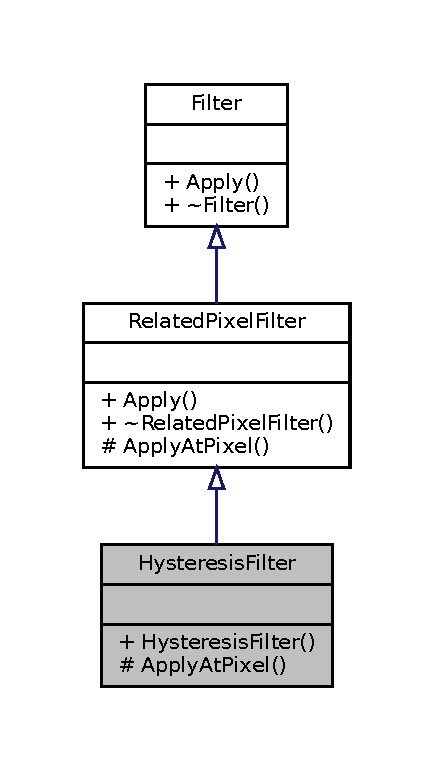
\includegraphics[width=208pt]{classHysteresisFilter__inherit__graph}
\end{center}
\end{figure}


Collaboration diagram for Hysteresis\+Filter\+:\nopagebreak
\begin{figure}[H]
\begin{center}
\leavevmode
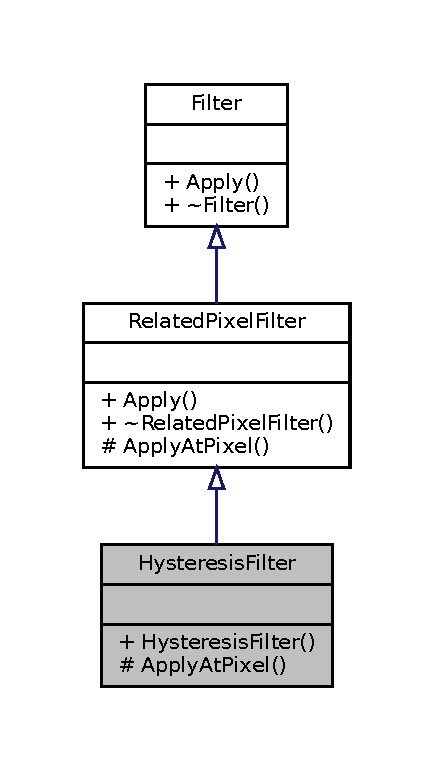
\includegraphics[width=208pt]{classHysteresisFilter__coll__graph}
\end{center}
\end{figure}
\subsection*{Public Member Functions}
\begin{DoxyCompactItemize}
\item 
\hyperlink{classHysteresisFilter_add3251eef42f477d14fb9fae1ba40e95}{Hysteresis\+Filter} (float weak\+Value, float strong\+Value)
\begin{DoxyCompactList}\small\item\em Constructor of a \hyperlink{classHysteresisFilter}{Hysteresis\+Filter} with a specified weak and strong value to classify pixels with. \end{DoxyCompactList}\end{DoxyCompactItemize}
\subsection*{Protected Member Functions}
\begin{DoxyCompactItemize}
\item 
std\+::vector$<$ \hyperlink{classColor}{Color} $>$ \hyperlink{classHysteresisFilter_a43990169f3f075ba8063c21ae83a0fc3}{Apply\+At\+Pixel} (const std\+::vector$<$ \hyperlink{classImage}{Image} $\ast$$>$ original, int x, int y)
\begin{DoxyCompactList}\small\item\em Modify an image by applying the effects of a Hysteresis filter to the pixel located at (x, y) in an instance of the \hyperlink{classImage}{Image} class. \end{DoxyCompactList}\end{DoxyCompactItemize}


\subsection{Detailed Description}
A class that can be used to apply a Hysteresis \hyperlink{classFilter}{Filter} to an instance of the \hyperlink{classImage}{Image} class. 

\subsection{Constructor \& Destructor Documentation}
\mbox{\Hypertarget{classHysteresisFilter_add3251eef42f477d14fb9fae1ba40e95}\label{classHysteresisFilter_add3251eef42f477d14fb9fae1ba40e95}} 
\index{Hysteresis\+Filter@{Hysteresis\+Filter}!Hysteresis\+Filter@{Hysteresis\+Filter}}
\index{Hysteresis\+Filter@{Hysteresis\+Filter}!Hysteresis\+Filter@{Hysteresis\+Filter}}
\subsubsection{\texorpdfstring{Hysteresis\+Filter()}{HysteresisFilter()}}
{\footnotesize\ttfamily Hysteresis\+Filter\+::\+Hysteresis\+Filter (\begin{DoxyParamCaption}\item[{float}]{weak\+Value = {\ttfamily 25.0},  }\item[{float}]{strong\+Value = {\ttfamily 255.0} }\end{DoxyParamCaption})}



Constructor of a \hyperlink{classHysteresisFilter}{Hysteresis\+Filter} with a specified weak and strong value to classify pixels with. 


\begin{DoxyParams}[1]{Parameters}
\mbox{\tt in}  & {\em weak\+Value} & A float value that represents the weak threshold values to classify pixels. \\
\hline
\mbox{\tt in}  & {\em strong\+Value} & A float value that represents the high threshold values to classify pixels.\\
\hline
\end{DoxyParams}
\begin{DoxyReturn}{Returns}
An instance of a \hyperlink{classHysteresisFilter}{Hysteresis\+Filter} with a specified weak and strong value to classify pixels with. 
\end{DoxyReturn}


\subsection{Member Function Documentation}
\mbox{\Hypertarget{classHysteresisFilter_a43990169f3f075ba8063c21ae83a0fc3}\label{classHysteresisFilter_a43990169f3f075ba8063c21ae83a0fc3}} 
\index{Hysteresis\+Filter@{Hysteresis\+Filter}!Apply\+At\+Pixel@{Apply\+At\+Pixel}}
\index{Apply\+At\+Pixel@{Apply\+At\+Pixel}!Hysteresis\+Filter@{Hysteresis\+Filter}}
\subsubsection{\texorpdfstring{Apply\+At\+Pixel()}{ApplyAtPixel()}}
{\footnotesize\ttfamily std\+::vector$<$ \hyperlink{classColor}{Color} $>$ Hysteresis\+Filter\+::\+Apply\+At\+Pixel (\begin{DoxyParamCaption}\item[{const std\+::vector$<$ \hyperlink{classImage}{Image} $\ast$$>$}]{original,  }\item[{int}]{x,  }\item[{int}]{y }\end{DoxyParamCaption})\hspace{0.3cm}{\ttfamily [protected]}, {\ttfamily [virtual]}}



Modify an image by applying the effects of a Hysteresis filter to the pixel located at (x, y) in an instance of the \hyperlink{classImage}{Image} class. 


\begin{DoxyParams}[1]{Parameters}
\mbox{\tt in}  & {\em original} & A vector of pointers to instances of the \hyperlink{classImage}{Image} class to be able to access the pixels of the original image. \\
\hline
\mbox{\tt in}  & {\em x} & An integer representing the x-\/coordinate of the pixel in the image. \\
\hline
\mbox{\tt in}  & {\em y} & An integer representing the y-\/coordinate of the pixel in the image.\\
\hline
\end{DoxyParams}
\begin{DoxyReturn}{Returns}
A vector of instances of the \hyperlink{classColor}{Color} class with each \hyperlink{classColor}{Color} object in the vector representing a new \hyperlink{classColor}{Color} for a different pixel in the image. 
\end{DoxyReturn}


Implements \hyperlink{classRelatedPixelFilter_a4701695c3b2ca7fdcc41b3d03c5840df}{Related\+Pixel\+Filter}.



The documentation for this class was generated from the following files\+:\begin{DoxyCompactItemize}
\item 
/home/user/repo/project/\+Image\+Processing/\hyperlink{hysteresis__filter_8h}{hysteresis\+\_\+filter.\+h}\item 
/home/user/repo/project/\+Image\+Processing/\hyperlink{hysteresis__filter_8cc}{hysteresis\+\_\+filter.\+cc}\end{DoxyCompactItemize}

\hypertarget{classICameraController}{}\section{I\+Camera\+Controller Class Reference}
\label{classICameraController}\index{I\+Camera\+Controller@{I\+Camera\+Controller}}


The \hyperlink{classCamera}{Camera} Controller class controls and allows for monitoring of all cameras.  




{\ttfamily \#include $<$camera\+\_\+controller.\+h$>$}



Inheritance diagram for I\+Camera\+Controller\+:\nopagebreak
\begin{figure}[H]
\begin{center}
\leavevmode
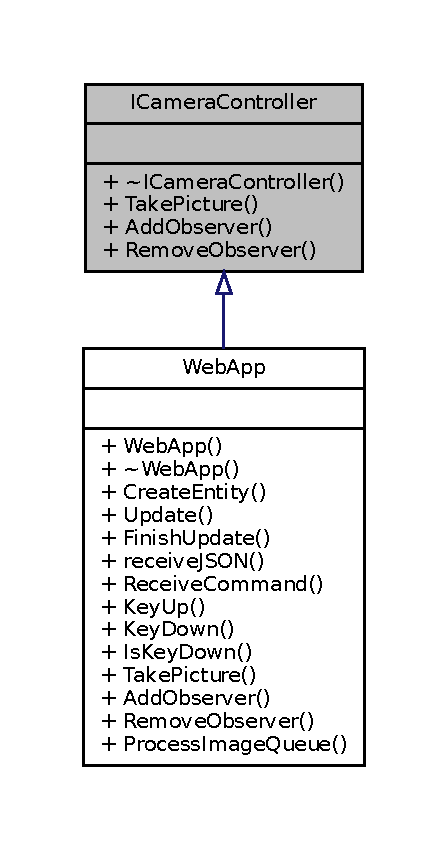
\includegraphics[width=215pt]{classICameraController__inherit__graph}
\end{center}
\end{figure}


Collaboration diagram for I\+Camera\+Controller\+:\nopagebreak
\begin{figure}[H]
\begin{center}
\leavevmode
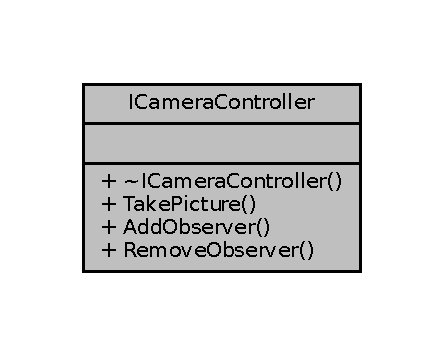
\includegraphics[width=213pt]{classICameraController__coll__graph}
\end{center}
\end{figure}
\subsection*{Public Member Functions}
\begin{DoxyCompactItemize}
\item 
\mbox{\Hypertarget{classICameraController_a7f1b88c7e023ad218d461684dc0d4fe5}\label{classICameraController_a7f1b88c7e023ad218d461684dc0d4fe5}} 
virtual \hyperlink{classICameraController_a7f1b88c7e023ad218d461684dc0d4fe5}{$\sim$\+I\+Camera\+Controller} ()
\begin{DoxyCompactList}\small\item\em Destructor. \end{DoxyCompactList}\item 
\mbox{\Hypertarget{classICameraController_af9fff22819969ca260f7f098f0cdebf4}\label{classICameraController_af9fff22819969ca260f7f098f0cdebf4}} 
virtual void \hyperlink{classICameraController_af9fff22819969ca260f7f098f0cdebf4}{Take\+Picture} (int camera\+Id)=0
\begin{DoxyCompactList}\small\item\em To take a picture with a specific camera, pass in the camera id. \end{DoxyCompactList}\item 
\mbox{\Hypertarget{classICameraController_ad3cf56dc052984b0e31e602f344c35db}\label{classICameraController_ad3cf56dc052984b0e31e602f344c35db}} 
virtual void \hyperlink{classICameraController_ad3cf56dc052984b0e31e602f344c35db}{Add\+Observer} (\hyperlink{classICameraObserver}{I\+Camera\+Observer} \&observer)=0
\begin{DoxyCompactList}\small\item\em Adds a camera observer to monitor cameras. \end{DoxyCompactList}\item 
\mbox{\Hypertarget{classICameraController_a5013bc29f6a0e7794a97646d868bf809}\label{classICameraController_a5013bc29f6a0e7794a97646d868bf809}} 
virtual void \hyperlink{classICameraController_a5013bc29f6a0e7794a97646d868bf809}{Remove\+Observer} (\hyperlink{classICameraObserver}{I\+Camera\+Observer} \&observer)=0
\begin{DoxyCompactList}\small\item\em Removes a camera observer. \end{DoxyCompactList}\end{DoxyCompactItemize}


\subsection{Detailed Description}
The \hyperlink{classCamera}{Camera} Controller class controls and allows for monitoring of all cameras. 

The documentation for this class was generated from the following file\+:\begin{DoxyCompactItemize}
\item 
/home/user/repo/project/src/camera\+\_\+controller.\+h\end{DoxyCompactItemize}

\hypertarget{classICameraObserver}{}\section{I\+Camera\+Observer Class Reference}
\label{classICameraObserver}\index{I\+Camera\+Observer@{I\+Camera\+Observer}}


A \hyperlink{classCamera}{Camera} Observer monitors results from all cameras. It will process the pictures returned asynchronously and act on results.  




{\ttfamily \#include $<$camera\+\_\+controller.\+h$>$}



Inheritance diagram for I\+Camera\+Observer\+:\nopagebreak
\begin{figure}[H]
\begin{center}
\leavevmode
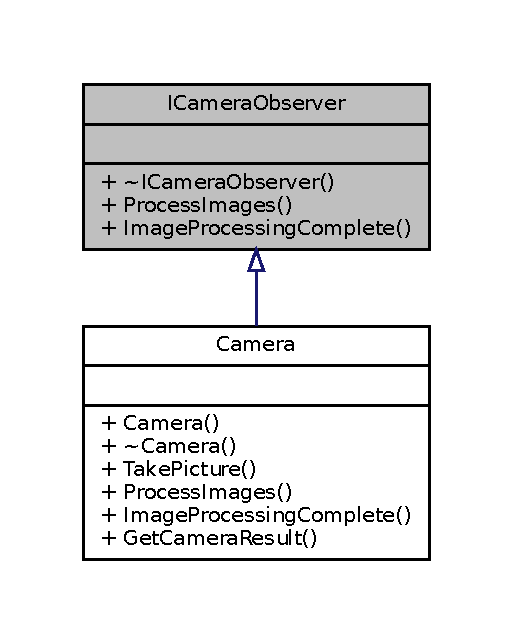
\includegraphics[width=246pt]{classICameraObserver__inherit__graph}
\end{center}
\end{figure}


Collaboration diagram for I\+Camera\+Observer\+:\nopagebreak
\begin{figure}[H]
\begin{center}
\leavevmode
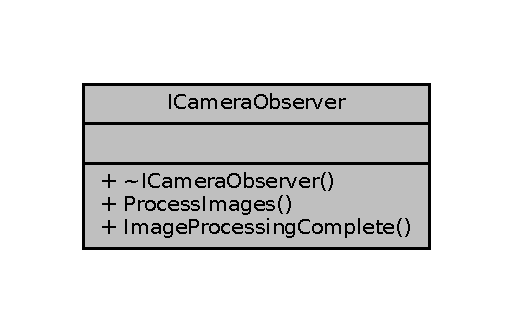
\includegraphics[width=246pt]{classICameraObserver__coll__graph}
\end{center}
\end{figure}
\subsection*{Public Member Functions}
\begin{DoxyCompactItemize}
\item 
\mbox{\Hypertarget{classICameraObserver_a19344cb93ca790a0311c9c7bcc6e8eec}\label{classICameraObserver_a19344cb93ca790a0311c9c7bcc6e8eec}} 
virtual \hyperlink{classICameraObserver_a19344cb93ca790a0311c9c7bcc6e8eec}{$\sim$\+I\+Camera\+Observer} ()
\begin{DoxyCompactList}\small\item\em Destructor. \end{DoxyCompactList}\item 
virtual \hyperlink{classICameraResult}{I\+Camera\+Result} $\ast$ \hyperlink{classICameraObserver_aec871459f2c429b4334769021b72ec34}{Process\+Images} (int camera\+Id, double x\+Pos, double y\+Pos, double z\+Pos, const std\+::vector$<$ \hyperlink{structRawCameraImage}{Raw\+Camera\+Image} $>$ \&images, picojson\+::object \&details) const =0
\item 
\mbox{\Hypertarget{classICameraObserver_a7d261bd08d570d05032e61b2d5252c88}\label{classICameraObserver_a7d261bd08d570d05032e61b2d5252c88}} 
virtual void \hyperlink{classICameraObserver_a7d261bd08d570d05032e61b2d5252c88}{Image\+Processing\+Complete} (\hyperlink{classICameraResult}{I\+Camera\+Result} $\ast$result)=0
\begin{DoxyCompactList}\small\item\em After the asynchronous image processing is done, this method is called to synchronize the results with the simulation update loop. \end{DoxyCompactList}\end{DoxyCompactItemize}


\subsection{Detailed Description}
A \hyperlink{classCamera}{Camera} Observer monitors results from all cameras. It will process the pictures returned asynchronously and act on results. 

\subsection{Member Function Documentation}
\mbox{\Hypertarget{classICameraObserver_aec871459f2c429b4334769021b72ec34}\label{classICameraObserver_aec871459f2c429b4334769021b72ec34}} 
\index{I\+Camera\+Observer@{I\+Camera\+Observer}!Process\+Images@{Process\+Images}}
\index{Process\+Images@{Process\+Images}!I\+Camera\+Observer@{I\+Camera\+Observer}}
\subsubsection{\texorpdfstring{Process\+Images()}{ProcessImages()}}
{\footnotesize\ttfamily virtual \hyperlink{classICameraResult}{I\+Camera\+Result}$\ast$ I\+Camera\+Observer\+::\+Process\+Images (\begin{DoxyParamCaption}\item[{int}]{camera\+Id,  }\item[{double}]{x\+Pos,  }\item[{double}]{y\+Pos,  }\item[{double}]{z\+Pos,  }\item[{const std\+::vector$<$ \hyperlink{structRawCameraImage}{Raw\+Camera\+Image} $>$ \&}]{images,  }\item[{picojson\+::object \&}]{details }\end{DoxyParamCaption}) const\hspace{0.3cm}{\ttfamily [pure virtual]}}

Processes images asynchronously after a picture has been taken. This method will pass in the camera position and the raw images stored in jpg format. Do all your image processing here so that it does not slow down your simulation. The result will be passed to the Image\+Processing\+Complete(...) method. 

Implemented in \hyperlink{classCamera_a792611ad34a1c595b61b7c72ce1d5e32}{Camera}.



The documentation for this class was generated from the following file\+:\begin{DoxyCompactItemize}
\item 
/home/user/repo/project/src/camera\+\_\+controller.\+h\end{DoxyCompactItemize}

\hypertarget{classICameraResult}{}\section{I\+Camera\+Result Class Reference}
\label{classICameraResult}\index{I\+Camera\+Result@{I\+Camera\+Result}}


The result returned from the image processing.  




{\ttfamily \#include $<$camera\+\_\+controller.\+h$>$}



Inheritance diagram for I\+Camera\+Result\+:\nopagebreak
\begin{figure}[H]
\begin{center}
\leavevmode
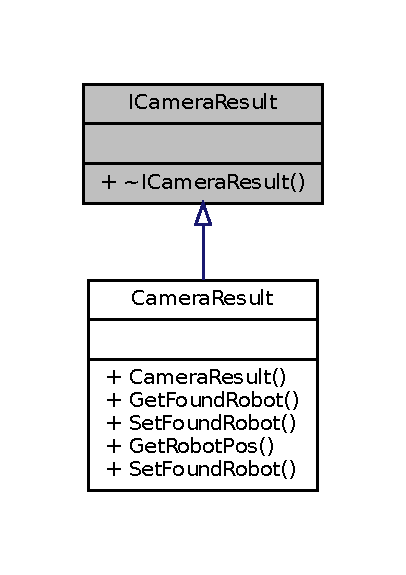
\includegraphics[width=195pt]{classICameraResult__inherit__graph}
\end{center}
\end{figure}


Collaboration diagram for I\+Camera\+Result\+:\nopagebreak
\begin{figure}[H]
\begin{center}
\leavevmode
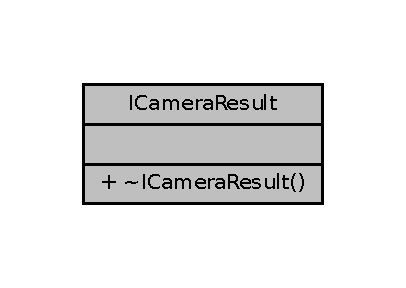
\includegraphics[width=195pt]{classICameraResult__coll__graph}
\end{center}
\end{figure}
\subsection*{Public Member Functions}
\begin{DoxyCompactItemize}
\item 
\mbox{\Hypertarget{classICameraResult_a6c8f4f6c3748c00236bd588cf9410f8b}\label{classICameraResult_a6c8f4f6c3748c00236bd588cf9410f8b}} 
virtual \hyperlink{classICameraResult_a6c8f4f6c3748c00236bd588cf9410f8b}{$\sim$\+I\+Camera\+Result} ()
\begin{DoxyCompactList}\small\item\em destructor \end{DoxyCompactList}\end{DoxyCompactItemize}


\subsection{Detailed Description}
The result returned from the image processing. 

The documentation for this class was generated from the following file\+:\begin{DoxyCompactItemize}
\item 
/home/user/repo/project/src/camera\+\_\+controller.\+h\end{DoxyCompactItemize}

\hypertarget{classIDrone}{}\section{I\+Drone Class Reference}
\label{classIDrone}\index{I\+Drone@{I\+Drone}}


Inheritance diagram for I\+Drone\+:\nopagebreak
\begin{figure}[H]
\begin{center}
\leavevmode
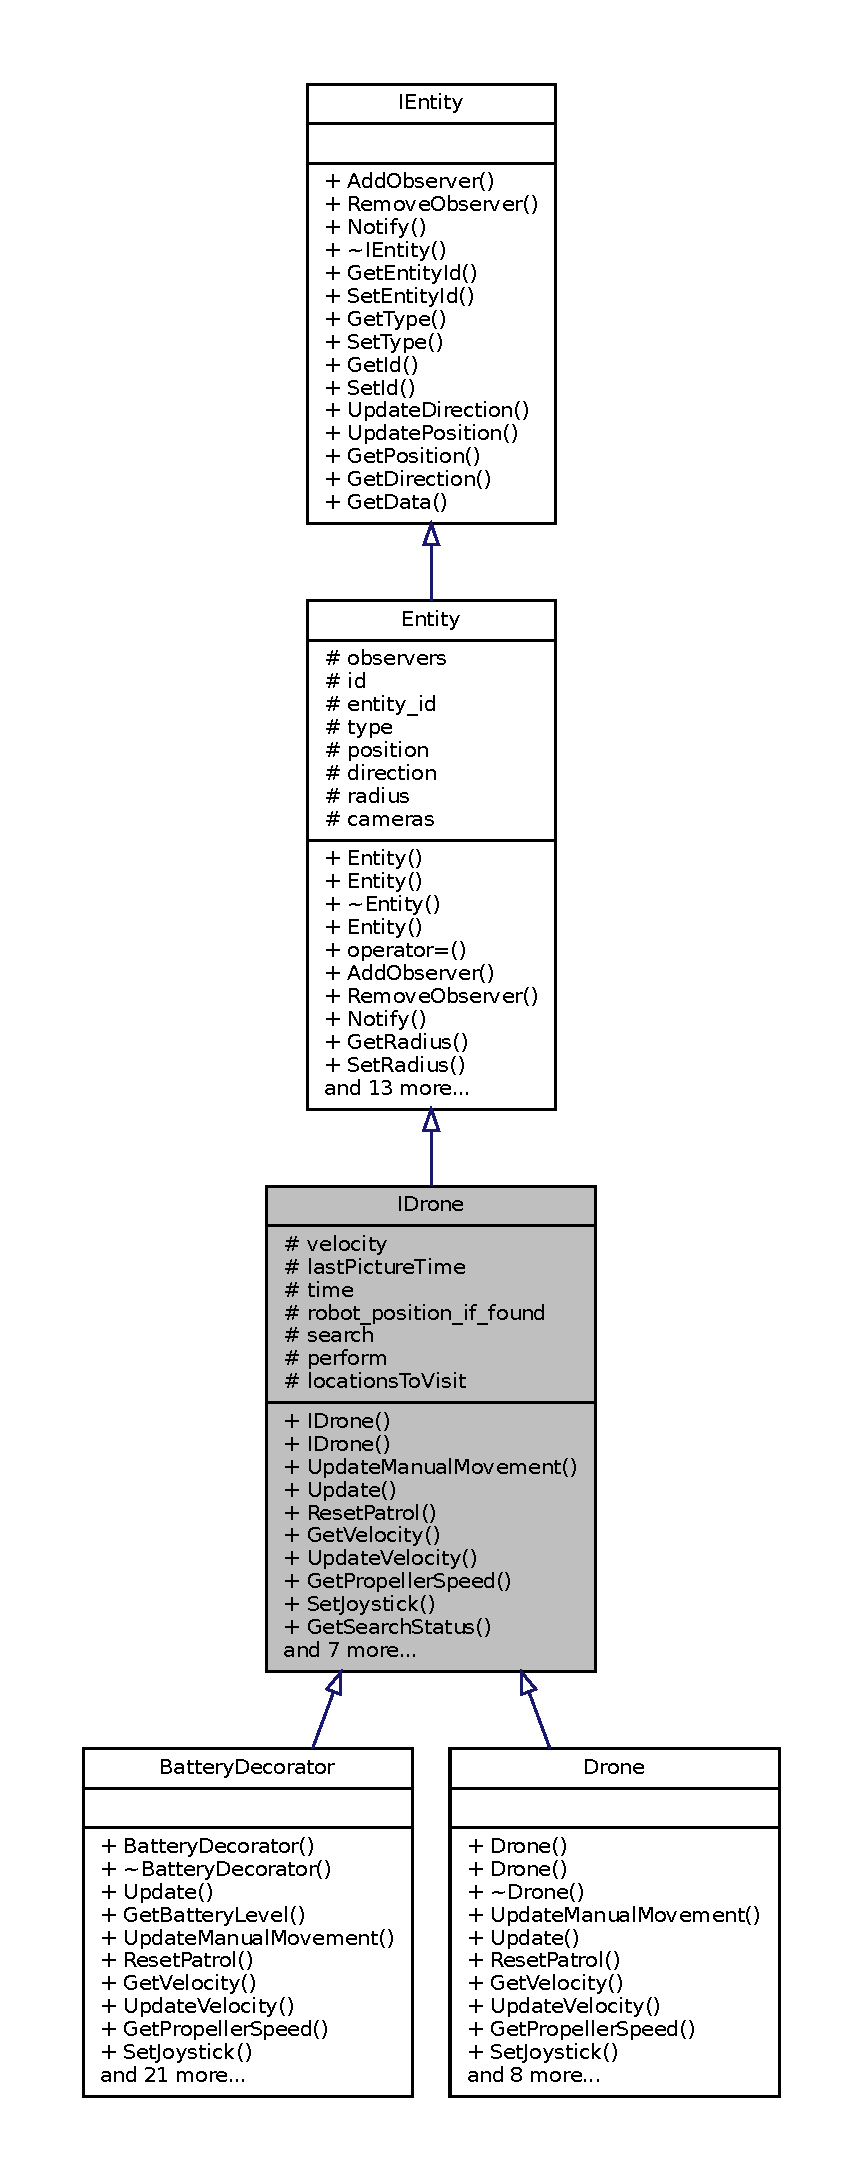
\includegraphics[height=550pt]{classIDrone__inherit__graph}
\end{center}
\end{figure}


Collaboration diagram for I\+Drone\+:\nopagebreak
\begin{figure}[H]
\begin{center}
\leavevmode
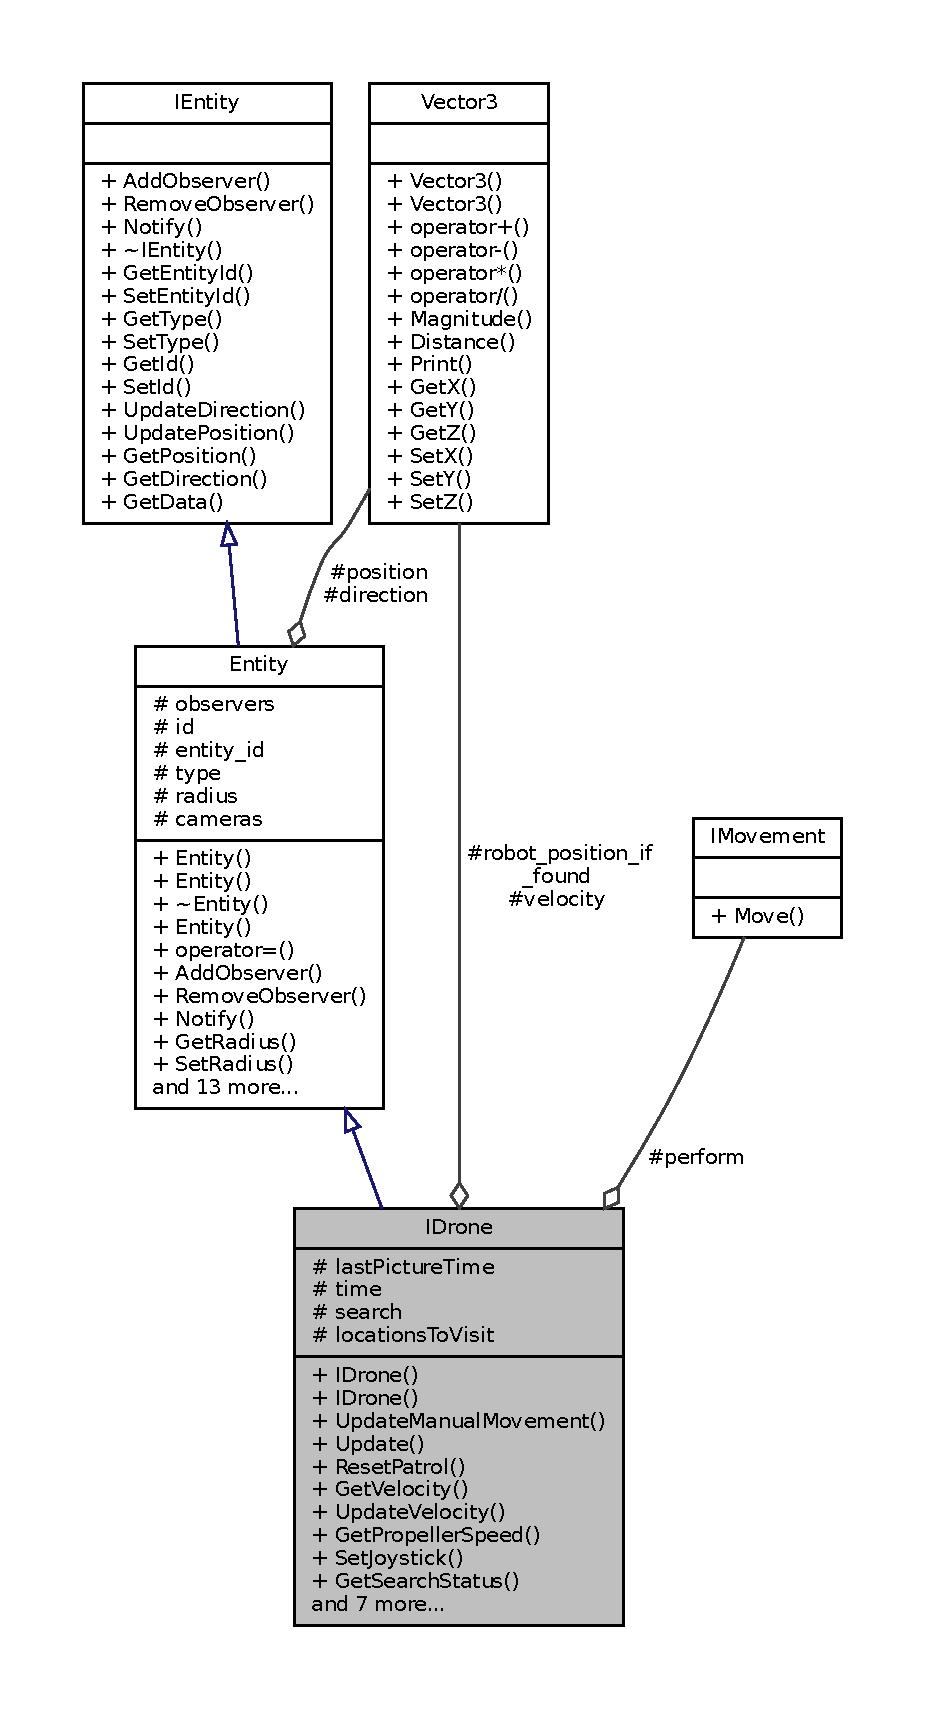
\includegraphics[height=550pt]{classIDrone__coll__graph}
\end{center}
\end{figure}
\subsection*{Public Member Functions}
\begin{DoxyCompactItemize}
\item 
\mbox{\Hypertarget{classIDrone_a28f6e8348bbf76a50009dd1577e616c2}\label{classIDrone_a28f6e8348bbf76a50009dd1577e616c2}} 
\hyperlink{classIDrone_a28f6e8348bbf76a50009dd1577e616c2}{I\+Drone} ()
\begin{DoxyCompactList}\small\item\em empty constructor \end{DoxyCompactList}\item 
\hyperlink{classIDrone_a7376a746197d7d24f09b8ad94fcee465}{I\+Drone} (picojson\+::object \&obj)
\begin{DoxyCompactList}\small\item\em Constructor. \end{DoxyCompactList}\item 
virtual void \hyperlink{classIDrone_a82486b4192f6ccf8b3d93fbb9101f2dd}{Update\+Manual\+Movement} (double dt)=0
\begin{DoxyCompactList}\small\item\em Moves based on keyboard inputs. \end{DoxyCompactList}\item 
virtual void \hyperlink{classIDrone_a6d840d60cda9a985b94af42ef54520b7}{Update} (double dt)=0
\begin{DoxyCompactList}\small\item\em calculates the new position of the drone based on Euler´s integration \end{DoxyCompactList}\item 
\mbox{\Hypertarget{classIDrone_aa7f5edb37f005c3afc94213eeee75283}\label{classIDrone_aa7f5edb37f005c3afc94213eeee75283}} 
virtual void \hyperlink{classIDrone_aa7f5edb37f005c3afc94213eeee75283}{Reset\+Patrol} ()=0
\begin{DoxyCompactList}\small\item\em Calculates the new patrol movement if we are still searching for the robot and have switch between manual and automatic movement. \end{DoxyCompactList}\item 
virtual \hyperlink{classVector3}{Vector3} \hyperlink{classIDrone_abad6c0adb60d6deceb13f30687fed57b}{Get\+Velocity} () const =0
\begin{DoxyCompactList}\small\item\em getter for the velocity of the drone \end{DoxyCompactList}\item 
virtual void \hyperlink{classIDrone_a5cc88b8205adaeea8f71c822d08e1607}{Update\+Velocity} (const \hyperlink{classVector3}{Vector3} \&new\+Dir)=0
\begin{DoxyCompactList}\small\item\em Updates the velocity of the drone. \end{DoxyCompactList}\item 
virtual double \hyperlink{classIDrone_a60a9a7eb90bf13100d66cb47b99830ed}{Get\+Propeller\+Speed} (int index)=0
\begin{DoxyCompactList}\small\item\em getter for the speed of one of the legs of the drone \end{DoxyCompactList}\item 
virtual void \hyperlink{classIDrone_a8414edd320f25869fb04a880eae0d554}{Set\+Joystick} (double x, double y, double z, double rotate)=0
\begin{DoxyCompactList}\small\item\em setter for the direction of the drone based on manual movement \end{DoxyCompactList}\item 
virtual bool \hyperlink{classIDrone_aed9abde2152408ef3483da57f24c4006}{Get\+Search\+Status} () const =0
\begin{DoxyCompactList}\small\item\em getter for the state of drone´s search (robot found or Not) \end{DoxyCompactList}\item 
virtual void \hyperlink{classIDrone_ac6f580814e7091ea64ecf2a7137b8120}{Set\+Search\+Status} (bool status)=0
\begin{DoxyCompactList}\small\item\em setter for the state of drone´s search (robot found or Not) \end{DoxyCompactList}\item 
virtual float \hyperlink{classIDrone_a112d19971ac7d94dba9e2f25ad667c0d}{Get\+Last\+Picture\+Time} () const =0
\begin{DoxyCompactList}\small\item\em getter for the last time drone took a pic \end{DoxyCompactList}\item 
virtual void \hyperlink{classIDrone_aace45f6d9a77bfc8c61bd0ffc30a3b8e}{Set\+Last\+Picture\+Time} (float time\+Pic)=0
\begin{DoxyCompactList}\small\item\em setter for the last time drone took a pic \end{DoxyCompactList}\item 
virtual float \hyperlink{classIDrone_a18809d1b0626ba66984ef3a91ffb644c}{Get\+Time} () const =0
\begin{DoxyCompactList}\small\item\em getter for the time elapsed \end{DoxyCompactList}\item 
virtual void \hyperlink{classIDrone_a0ca36885fd79fbf2efa3909771218d56}{Set\+Time} (float t)=0
\begin{DoxyCompactList}\small\item\em setter for the time elapsed \end{DoxyCompactList}\item 
virtual \hyperlink{classVector3}{Vector3} \hyperlink{classIDrone_a1c3f5e712a97625c74c35952b930d68d}{Get\+Robot\+Pos} () const =0
\begin{DoxyCompactList}\small\item\em A method to get the robot x y z position. \end{DoxyCompactList}\item 
virtual void \hyperlink{classIDrone_a5851e679bf3c915e93165377cb5c8815}{Set\+Robot\+Pos} (\hyperlink{classVector3}{Vector3} pos)=0
\begin{DoxyCompactList}\small\item\em A method to set the robot x y z position. \end{DoxyCompactList}\end{DoxyCompactItemize}
\subsection*{Protected Attributes}
\begin{DoxyCompactItemize}
\item 
\mbox{\Hypertarget{classIDrone_aade2e69c0b9e11cc8d3698a839eefe1f}\label{classIDrone_aade2e69c0b9e11cc8d3698a839eefe1f}} 
\hyperlink{classVector3}{Vector3} \hyperlink{classIDrone_aade2e69c0b9e11cc8d3698a839eefe1f}{velocity}
\begin{DoxyCompactList}\small\item\em vector3 representing the velocity of the drone \end{DoxyCompactList}\item 
\mbox{\Hypertarget{classIDrone_ab5f413dcf3f8b8aae98e40d8a9882505}\label{classIDrone_ab5f413dcf3f8b8aae98e40d8a9882505}} 
float \hyperlink{classIDrone_ab5f413dcf3f8b8aae98e40d8a9882505}{last\+Picture\+Time} = 0.\+0
\begin{DoxyCompactList}\small\item\em float representing time of last picture taken \end{DoxyCompactList}\item 
\mbox{\Hypertarget{classIDrone_a2afb078f920b717e8307afa11e88bb3b}\label{classIDrone_a2afb078f920b717e8307afa11e88bb3b}} 
float \hyperlink{classIDrone_a2afb078f920b717e8307afa11e88bb3b}{time} = 0.\+0
\begin{DoxyCompactList}\small\item\em float representing time ellapsed \end{DoxyCompactList}\item 
\mbox{\Hypertarget{classIDrone_a6621d481350659d9c7ac17f57513eda9}\label{classIDrone_a6621d481350659d9c7ac17f57513eda9}} 
\hyperlink{classVector3}{Vector3} \hyperlink{classIDrone_a6621d481350659d9c7ac17f57513eda9}{robot\+\_\+position\+\_\+if\+\_\+found}
\begin{DoxyCompactList}\small\item\em vector3 representing the robot position iff found \end{DoxyCompactList}\item 
\mbox{\Hypertarget{classIDrone_ac17ac938c4991f17ccd97cc93102fa65}\label{classIDrone_ac17ac938c4991f17ccd97cc93102fa65}} 
bool \hyperlink{classIDrone_ac17ac938c4991f17ccd97cc93102fa65}{search} = false
\begin{DoxyCompactList}\small\item\em boolean representing if we have found \hyperlink{classDrone}{Drone} or not \end{DoxyCompactList}\item 
\mbox{\Hypertarget{classIDrone_a208565b0b4c7f5a485a7d9a0e9ca23d0}\label{classIDrone_a208565b0b4c7f5a485a7d9a0e9ca23d0}} 
\hyperlink{classIMovement}{I\+Movement} $\ast$ \hyperlink{classIDrone_a208565b0b4c7f5a485a7d9a0e9ca23d0}{perform}
\begin{DoxyCompactList}\small\item\em I\+Movement$\ast$ A pointer to a movement strategy for the Done to move around the scene with. \end{DoxyCompactList}\item 
\mbox{\Hypertarget{classIDrone_a5c8bd9edded1b4b4ef9cde53ce66f2cc}\label{classIDrone_a5c8bd9edded1b4b4ef9cde53ce66f2cc}} 
std\+::queue$<$ \hyperlink{classVector3}{Vector3} $>$ \hyperlink{classIDrone_a5c8bd9edded1b4b4ef9cde53ce66f2cc}{locations\+To\+Visit}
\begin{DoxyCompactList}\small\item\em std\+::queue$<$\+Vector3$>$ A queue representing locations the \hyperlink{classDrone}{Drone} should visit on the map \end{DoxyCompactList}\end{DoxyCompactItemize}


\subsection{Constructor \& Destructor Documentation}
\mbox{\Hypertarget{classIDrone_a7376a746197d7d24f09b8ad94fcee465}\label{classIDrone_a7376a746197d7d24f09b8ad94fcee465}} 
\index{I\+Drone@{I\+Drone}!I\+Drone@{I\+Drone}}
\index{I\+Drone@{I\+Drone}!I\+Drone@{I\+Drone}}
\subsubsection{\texorpdfstring{I\+Drone()}{IDrone()}}
{\footnotesize\ttfamily I\+Drone\+::\+I\+Drone (\begin{DoxyParamCaption}\item[{picojson\+::object \&}]{obj }\end{DoxyParamCaption})\hspace{0.3cm}{\ttfamily [inline]}}



Constructor. 


\begin{DoxyParams}[1]{Parameters}
\mbox{\tt in}  & {\em object} & picson object Object that we want to retrive info from \\
\hline
\end{DoxyParams}


\subsection{Member Function Documentation}
\mbox{\Hypertarget{classIDrone_a112d19971ac7d94dba9e2f25ad667c0d}\label{classIDrone_a112d19971ac7d94dba9e2f25ad667c0d}} 
\index{I\+Drone@{I\+Drone}!Get\+Last\+Picture\+Time@{Get\+Last\+Picture\+Time}}
\index{Get\+Last\+Picture\+Time@{Get\+Last\+Picture\+Time}!I\+Drone@{I\+Drone}}
\subsubsection{\texorpdfstring{Get\+Last\+Picture\+Time()}{GetLastPictureTime()}}
{\footnotesize\ttfamily virtual float I\+Drone\+::\+Get\+Last\+Picture\+Time (\begin{DoxyParamCaption}{ }\end{DoxyParamCaption}) const\hspace{0.3cm}{\ttfamily [pure virtual]}}



getter for the last time drone took a pic 

\begin{DoxyReturn}{Returns}
float representing time elapsed since that picture 
\end{DoxyReturn}


Implemented in \hyperlink{classDrone_a78de3dcbc6ae754e8874a8b65e8cd9ee}{Drone}, and \hyperlink{classBatteryDecorator_a661b3722c37ce7d9690e50724eac863e}{Battery\+Decorator}.

\mbox{\Hypertarget{classIDrone_a60a9a7eb90bf13100d66cb47b99830ed}\label{classIDrone_a60a9a7eb90bf13100d66cb47b99830ed}} 
\index{I\+Drone@{I\+Drone}!Get\+Propeller\+Speed@{Get\+Propeller\+Speed}}
\index{Get\+Propeller\+Speed@{Get\+Propeller\+Speed}!I\+Drone@{I\+Drone}}
\subsubsection{\texorpdfstring{Get\+Propeller\+Speed()}{GetPropellerSpeed()}}
{\footnotesize\ttfamily virtual double I\+Drone\+::\+Get\+Propeller\+Speed (\begin{DoxyParamCaption}\item[{int}]{index }\end{DoxyParamCaption})\hspace{0.3cm}{\ttfamily [pure virtual]}}



getter for the speed of one of the legs of the drone 

\begin{DoxyReturn}{Returns}
double representing the speed of the index propeller 
\end{DoxyReturn}


Implemented in \hyperlink{classDrone_a7b2fd7d3ed57cec48ebdcd09f97b83f7}{Drone}, and \hyperlink{classBatteryDecorator_a361154605b803347aea2422cae7d0183}{Battery\+Decorator}.

\mbox{\Hypertarget{classIDrone_a1c3f5e712a97625c74c35952b930d68d}\label{classIDrone_a1c3f5e712a97625c74c35952b930d68d}} 
\index{I\+Drone@{I\+Drone}!Get\+Robot\+Pos@{Get\+Robot\+Pos}}
\index{Get\+Robot\+Pos@{Get\+Robot\+Pos}!I\+Drone@{I\+Drone}}
\subsubsection{\texorpdfstring{Get\+Robot\+Pos()}{GetRobotPos()}}
{\footnotesize\ttfamily virtual \hyperlink{classVector3}{Vector3} I\+Drone\+::\+Get\+Robot\+Pos (\begin{DoxyParamCaption}{ }\end{DoxyParamCaption}) const\hspace{0.3cm}{\ttfamily [pure virtual]}}



A method to get the robot x y z position. 

\begin{DoxyReturn}{Returns}
Vector representing position where robot found 
\end{DoxyReturn}


Implemented in \hyperlink{classBatteryDecorator_ac9f7223d439db341e9765ea3d5584f4e}{Battery\+Decorator}, and \hyperlink{classDrone_afdba5de8493255a433d62382991dfe8e}{Drone}.

\mbox{\Hypertarget{classIDrone_aed9abde2152408ef3483da57f24c4006}\label{classIDrone_aed9abde2152408ef3483da57f24c4006}} 
\index{I\+Drone@{I\+Drone}!Get\+Search\+Status@{Get\+Search\+Status}}
\index{Get\+Search\+Status@{Get\+Search\+Status}!I\+Drone@{I\+Drone}}
\subsubsection{\texorpdfstring{Get\+Search\+Status()}{GetSearchStatus()}}
{\footnotesize\ttfamily virtual bool I\+Drone\+::\+Get\+Search\+Status (\begin{DoxyParamCaption}{ }\end{DoxyParamCaption}) const\hspace{0.3cm}{\ttfamily [pure virtual]}}



getter for the state of drone´s search (robot found or Not) 

\begin{DoxyReturn}{Returns}
boolean true if we have found robot and are moving torwards it, false otherwise 
\end{DoxyReturn}


Implemented in \hyperlink{classDrone_a9bfe1ce0aea1215da3072434ed8e8527}{Drone}, and \hyperlink{classBatteryDecorator_aa0358ef7a9aee0f4942d32ad15ce4675}{Battery\+Decorator}.

\mbox{\Hypertarget{classIDrone_a18809d1b0626ba66984ef3a91ffb644c}\label{classIDrone_a18809d1b0626ba66984ef3a91ffb644c}} 
\index{I\+Drone@{I\+Drone}!Get\+Time@{Get\+Time}}
\index{Get\+Time@{Get\+Time}!I\+Drone@{I\+Drone}}
\subsubsection{\texorpdfstring{Get\+Time()}{GetTime()}}
{\footnotesize\ttfamily virtual float I\+Drone\+::\+Get\+Time (\begin{DoxyParamCaption}{ }\end{DoxyParamCaption}) const\hspace{0.3cm}{\ttfamily [pure virtual]}}



getter for the time elapsed 

\begin{DoxyReturn}{Returns}
float representing time elapsed (sum of updates dt´s) 
\end{DoxyReturn}


Implemented in \hyperlink{classDrone_a0fde6a9a239da64ae102053c6404fe4d}{Drone}, and \hyperlink{classBatteryDecorator_a87cb6d468b6cd418775b4e01308fc0bf}{Battery\+Decorator}.

\mbox{\Hypertarget{classIDrone_abad6c0adb60d6deceb13f30687fed57b}\label{classIDrone_abad6c0adb60d6deceb13f30687fed57b}} 
\index{I\+Drone@{I\+Drone}!Get\+Velocity@{Get\+Velocity}}
\index{Get\+Velocity@{Get\+Velocity}!I\+Drone@{I\+Drone}}
\subsubsection{\texorpdfstring{Get\+Velocity()}{GetVelocity()}}
{\footnotesize\ttfamily virtual \hyperlink{classVector3}{Vector3} I\+Drone\+::\+Get\+Velocity (\begin{DoxyParamCaption}{ }\end{DoxyParamCaption}) const\hspace{0.3cm}{\ttfamily [pure virtual]}}



getter for the velocity of the drone 

\begin{DoxyReturn}{Returns}
vector3 representing the velocity of the drone 
\end{DoxyReturn}


Implemented in \hyperlink{classDrone_ac5adae4a3cbe2e39f577fa7da14407c7}{Drone}, and \hyperlink{classBatteryDecorator_a978565b772172669437ffec923349f32}{Battery\+Decorator}.

\mbox{\Hypertarget{classIDrone_a8414edd320f25869fb04a880eae0d554}\label{classIDrone_a8414edd320f25869fb04a880eae0d554}} 
\index{I\+Drone@{I\+Drone}!Set\+Joystick@{Set\+Joystick}}
\index{Set\+Joystick@{Set\+Joystick}!I\+Drone@{I\+Drone}}
\subsubsection{\texorpdfstring{Set\+Joystick()}{SetJoystick()}}
{\footnotesize\ttfamily virtual void I\+Drone\+::\+Set\+Joystick (\begin{DoxyParamCaption}\item[{double}]{x,  }\item[{double}]{y,  }\item[{double}]{z,  }\item[{double}]{rotate }\end{DoxyParamCaption})\hspace{0.3cm}{\ttfamily [pure virtual]}}



setter for the direction of the drone based on manual movement 


\begin{DoxyParams}[1]{Parameters}
\mbox{\tt in}  & {\em x} & double representing the direction on the x direction \\
\hline
\mbox{\tt in}  & {\em y} & double representing the direction on the y direction \\
\hline
\mbox{\tt in}  & {\em z} & double representing the direction on the z direction \\
\hline
\mbox{\tt in}  & {\em rotate} & double representing the rotation value of drone \\
\hline
\end{DoxyParams}


Implemented in \hyperlink{classDrone_a648ebd16d398c677918d94471010ddc6}{Drone}, and \hyperlink{classBatteryDecorator_abb1ece4f26ac33daefd53a56180721eb}{Battery\+Decorator}.

\mbox{\Hypertarget{classIDrone_aace45f6d9a77bfc8c61bd0ffc30a3b8e}\label{classIDrone_aace45f6d9a77bfc8c61bd0ffc30a3b8e}} 
\index{I\+Drone@{I\+Drone}!Set\+Last\+Picture\+Time@{Set\+Last\+Picture\+Time}}
\index{Set\+Last\+Picture\+Time@{Set\+Last\+Picture\+Time}!I\+Drone@{I\+Drone}}
\subsubsection{\texorpdfstring{Set\+Last\+Picture\+Time()}{SetLastPictureTime()}}
{\footnotesize\ttfamily virtual void I\+Drone\+::\+Set\+Last\+Picture\+Time (\begin{DoxyParamCaption}\item[{float}]{time\+Pic }\end{DoxyParamCaption})\hspace{0.3cm}{\ttfamily [pure virtual]}}



setter for the last time drone took a pic 


\begin{DoxyParams}[1]{Parameters}
\mbox{\tt in}  & {\em time\+Pic} & float representing time since last\+Picture \\
\hline
\end{DoxyParams}


Implemented in \hyperlink{classDrone_af639374e11eb02702665ba9f71697a01}{Drone}, and \hyperlink{classBatteryDecorator_abcaad479f82c6b8fcef4b511fb702d61}{Battery\+Decorator}.

\mbox{\Hypertarget{classIDrone_a5851e679bf3c915e93165377cb5c8815}\label{classIDrone_a5851e679bf3c915e93165377cb5c8815}} 
\index{I\+Drone@{I\+Drone}!Set\+Robot\+Pos@{Set\+Robot\+Pos}}
\index{Set\+Robot\+Pos@{Set\+Robot\+Pos}!I\+Drone@{I\+Drone}}
\subsubsection{\texorpdfstring{Set\+Robot\+Pos()}{SetRobotPos()}}
{\footnotesize\ttfamily virtual void I\+Drone\+::\+Set\+Robot\+Pos (\begin{DoxyParamCaption}\item[{\hyperlink{classVector3}{Vector3}}]{pos }\end{DoxyParamCaption})\hspace{0.3cm}{\ttfamily [pure virtual]}}



A method to set the robot x y z position. 


\begin{DoxyParams}[1]{Parameters}
\mbox{\tt in}  & {\em pos} & Vector representing position where robot found \\
\hline
\end{DoxyParams}


Implemented in \hyperlink{classBatteryDecorator_a183e98816461760d499366e112e5d0a6}{Battery\+Decorator}, and \hyperlink{classDrone_a384abec1f84c15ec1c5533d9ccc8b865}{Drone}.

\mbox{\Hypertarget{classIDrone_ac6f580814e7091ea64ecf2a7137b8120}\label{classIDrone_ac6f580814e7091ea64ecf2a7137b8120}} 
\index{I\+Drone@{I\+Drone}!Set\+Search\+Status@{Set\+Search\+Status}}
\index{Set\+Search\+Status@{Set\+Search\+Status}!I\+Drone@{I\+Drone}}
\subsubsection{\texorpdfstring{Set\+Search\+Status()}{SetSearchStatus()}}
{\footnotesize\ttfamily virtual void I\+Drone\+::\+Set\+Search\+Status (\begin{DoxyParamCaption}\item[{bool}]{status }\end{DoxyParamCaption})\hspace{0.3cm}{\ttfamily [pure virtual]}}



setter for the state of drone´s search (robot found or Not) 


\begin{DoxyParams}[1]{Parameters}
\mbox{\tt in}  & {\em status} & boolean true if we have found robot and are moving torwards it, false otherwise \\
\hline
\end{DoxyParams}


Implemented in \hyperlink{classDrone_a5349ad4b562b038a2d27ede3ed3fa80d}{Drone}, and \hyperlink{classBatteryDecorator_a41d8c8512cf82484120a9f3f951c4c2b}{Battery\+Decorator}.

\mbox{\Hypertarget{classIDrone_a0ca36885fd79fbf2efa3909771218d56}\label{classIDrone_a0ca36885fd79fbf2efa3909771218d56}} 
\index{I\+Drone@{I\+Drone}!Set\+Time@{Set\+Time}}
\index{Set\+Time@{Set\+Time}!I\+Drone@{I\+Drone}}
\subsubsection{\texorpdfstring{Set\+Time()}{SetTime()}}
{\footnotesize\ttfamily virtual void I\+Drone\+::\+Set\+Time (\begin{DoxyParamCaption}\item[{float}]{t }\end{DoxyParamCaption})\hspace{0.3cm}{\ttfamily [pure virtual]}}



setter for the time elapsed 


\begin{DoxyParams}[1]{Parameters}
\mbox{\tt in}  & {\em t} & float representing time elapsed (sum of updates dt´s) \\
\hline
\end{DoxyParams}


Implemented in \hyperlink{classDrone_a3c8e1ccbff90c7b5192679317f219061}{Drone}, and \hyperlink{classBatteryDecorator_abf7e2a2b4634330de27e7072236ffc5f}{Battery\+Decorator}.

\mbox{\Hypertarget{classIDrone_a6d840d60cda9a985b94af42ef54520b7}\label{classIDrone_a6d840d60cda9a985b94af42ef54520b7}} 
\index{I\+Drone@{I\+Drone}!Update@{Update}}
\index{Update@{Update}!I\+Drone@{I\+Drone}}
\subsubsection{\texorpdfstring{Update()}{Update()}}
{\footnotesize\ttfamily virtual void I\+Drone\+::\+Update (\begin{DoxyParamCaption}\item[{double}]{dt }\end{DoxyParamCaption})\hspace{0.3cm}{\ttfamily [pure virtual]}}



calculates the new position of the drone based on Euler´s integration 


\begin{DoxyParams}[1]{Parameters}
\mbox{\tt in}  & {\em dt} & period of time it has elapsed since last update \\
\hline
\end{DoxyParams}


Implemented in \hyperlink{classDrone_abc6b79ccc7fdbc3bec8d539fc836c04d}{Drone}, and \hyperlink{classBatteryDecorator_a92ea38b63e41d61d7392cb58a53fa8d9}{Battery\+Decorator}.

\mbox{\Hypertarget{classIDrone_a82486b4192f6ccf8b3d93fbb9101f2dd}\label{classIDrone_a82486b4192f6ccf8b3d93fbb9101f2dd}} 
\index{I\+Drone@{I\+Drone}!Update\+Manual\+Movement@{Update\+Manual\+Movement}}
\index{Update\+Manual\+Movement@{Update\+Manual\+Movement}!I\+Drone@{I\+Drone}}
\subsubsection{\texorpdfstring{Update\+Manual\+Movement()}{UpdateManualMovement()}}
{\footnotesize\ttfamily virtual void I\+Drone\+::\+Update\+Manual\+Movement (\begin{DoxyParamCaption}\item[{double}]{dt }\end{DoxyParamCaption})\hspace{0.3cm}{\ttfamily [pure virtual]}}



Moves based on keyboard inputs. 


\begin{DoxyParams}[1]{Parameters}
\mbox{\tt in}  & {\em dt} & period of time it has elapsed since last update \\
\hline
\end{DoxyParams}


Implemented in \hyperlink{classBatteryDecorator_a45babf9bc5484acb95701d361e89de9b}{Battery\+Decorator}, and \hyperlink{classDrone_aabfc6155cd0b8e14ae77c4659c090185}{Drone}.

\mbox{\Hypertarget{classIDrone_a5cc88b8205adaeea8f71c822d08e1607}\label{classIDrone_a5cc88b8205adaeea8f71c822d08e1607}} 
\index{I\+Drone@{I\+Drone}!Update\+Velocity@{Update\+Velocity}}
\index{Update\+Velocity@{Update\+Velocity}!I\+Drone@{I\+Drone}}
\subsubsection{\texorpdfstring{Update\+Velocity()}{UpdateVelocity()}}
{\footnotesize\ttfamily virtual void I\+Drone\+::\+Update\+Velocity (\begin{DoxyParamCaption}\item[{const \hyperlink{classVector3}{Vector3} \&}]{new\+Dir }\end{DoxyParamCaption})\hspace{0.3cm}{\ttfamily [pure virtual]}}



Updates the velocity of the drone. 


\begin{DoxyParams}[1]{Parameters}
\mbox{\tt in}  & {\em new\+Dir} & vector3 representing the new velocity of the object \\
\hline
\end{DoxyParams}


Implemented in \hyperlink{classDrone_a8ecc9a70f1d3907a79be433bfa9b5d68}{Drone}, and \hyperlink{classBatteryDecorator_aad635fd483288cdcc46892da5265ca49}{Battery\+Decorator}.



The documentation for this class was generated from the following file\+:\begin{DoxyCompactItemize}
\item 
/home/user/repo/project/src/\+Entity/\hyperlink{IDrone_8h}{I\+Drone.\+h}\end{DoxyCompactItemize}

\hypertarget{classIEntity}{}\section{I\+Entity Class Reference}
\label{classIEntity}\index{I\+Entity@{I\+Entity}}


Inheritance diagram for I\+Entity\+:\nopagebreak
\begin{figure}[H]
\begin{center}
\leavevmode
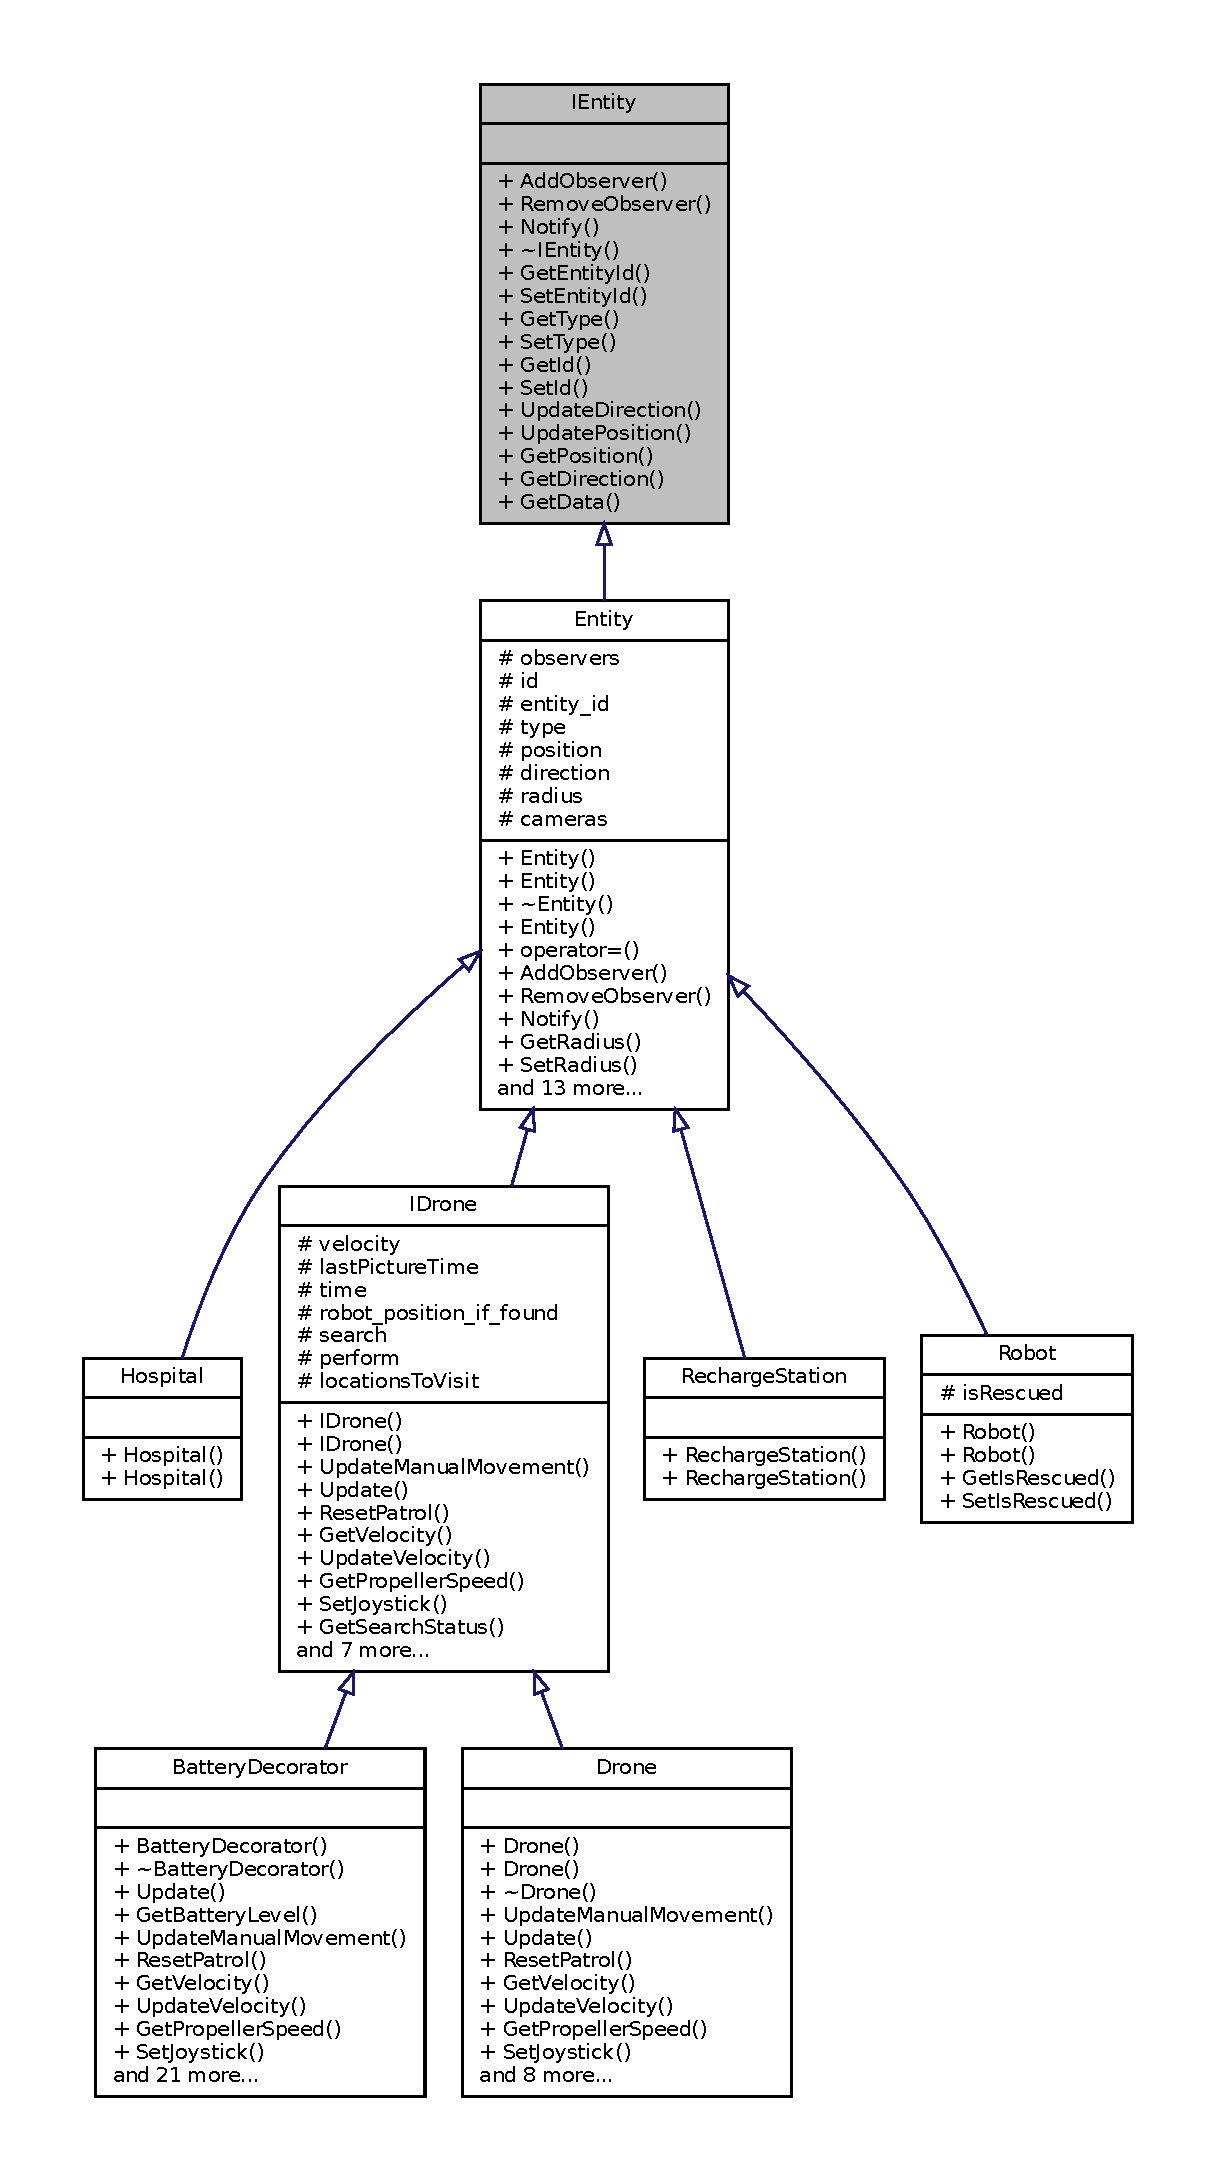
\includegraphics[height=550pt]{classIEntity__inherit__graph}
\end{center}
\end{figure}


Collaboration diagram for I\+Entity\+:\nopagebreak
\begin{figure}[H]
\begin{center}
\leavevmode
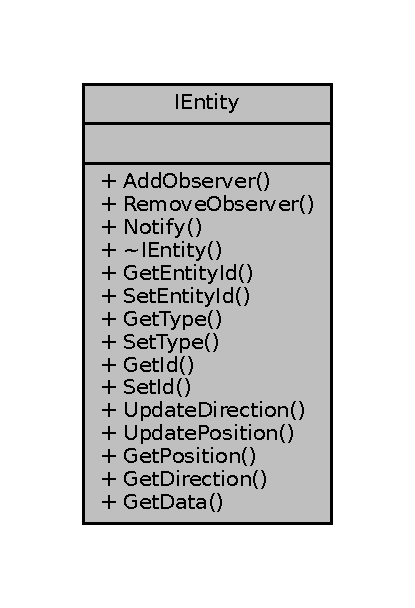
\includegraphics[width=199pt]{classIEntity__coll__graph}
\end{center}
\end{figure}
\subsection*{Public Member Functions}
\begin{DoxyCompactItemize}
\item 
virtual void \hyperlink{classIEntity_a0d682e3663a78b6b5fd3df8cd51aa321}{Add\+Observer} (\hyperlink{classIObserver}{I\+Observer} $\ast$new\+\_\+observer)=0
\begin{DoxyCompactList}\small\item\em Function that will add an observer to the entity. \end{DoxyCompactList}\item 
virtual void \hyperlink{classIEntity_a651f1ca9f1e494af74e3f580b1c118d6}{Remove\+Observer} (\hyperlink{classIObserver}{I\+Observer} $\ast$observer\+\_\+to\+\_\+remove)=0
\begin{DoxyCompactList}\small\item\em Function that will remove an observer from the entity. \end{DoxyCompactList}\item 
virtual void \hyperlink{classIEntity_acd19cac6fe0e65495f80d1962320e0c3}{Notify} (picojson\+::object \&notification)=0
\begin{DoxyCompactList}\small\item\em Function that will send a message to the observers of that entity so message gets notified to the UI. \end{DoxyCompactList}\item 
\mbox{\Hypertarget{classIEntity_a727892234e0efad23c7a399997dee974}\label{classIEntity_a727892234e0efad23c7a399997dee974}} 
virtual \hyperlink{classIEntity_a727892234e0efad23c7a399997dee974}{$\sim$\+I\+Entity} ()=default
\begin{DoxyCompactList}\small\item\em A virtual destructor needed to call sub-\/classes destructors. \end{DoxyCompactList}\item 
virtual int \hyperlink{classIEntity_a4359ee47413fa0b2940b3b0336e13861}{Get\+Entity\+Id} ()=0
\begin{DoxyCompactList}\small\item\em This will return the \hyperlink{classEntity}{Entity} Id, meaning the type of object (0 represents a drone) \end{DoxyCompactList}\item 
virtual void \hyperlink{classIEntity_a3a830862181cb0548d2aca83d908263e}{Set\+Entity\+Id} (int id2)=0
\begin{DoxyCompactList}\small\item\em This will set the \hyperlink{classEntity}{Entity} Id, meaning the type of object (0 represents a drone) \end{DoxyCompactList}\item 
virtual std\+::string \hyperlink{classIEntity_ac494bb9712d5a03495a1a95afdbd7153}{Get\+Type} ()=0
\begin{DoxyCompactList}\small\item\em This will return a string representing object type \char`\"{}drone\char`\"{}, \char`\"{}hospital\char`\"{}... \end{DoxyCompactList}\item 
virtual void \hyperlink{classIEntity_a49b3c54f94a93d4a9f96527ffb8982f5}{Set\+Type} (std\+::string \&name)=0
\begin{DoxyCompactList}\small\item\em This will set the object type \char`\"{}drone\char`\"{}, \char`\"{}hospital\char`\"{}... \end{DoxyCompactList}\item 
virtual int \hyperlink{classIEntity_ac3d60cc2fab1ccb61c1be92373e636d9}{Get\+Id} ()=0
\begin{DoxyCompactList}\small\item\em This will return an integer that represents the command in which the object was created. \end{DoxyCompactList}\item 
virtual void \hyperlink{classIEntity_a8c6af682e07f569ba2f164d214295c67}{Set\+Id} (int id2)=0
\begin{DoxyCompactList}\small\item\em This will set the command \# in which the object was created. \end{DoxyCompactList}\item 
virtual void \hyperlink{classIEntity_af24054e349dcdaea31a778427a34495d}{Update\+Direction} (const \hyperlink{classVector3}{Vector3} \&new\+Dir)=0
\begin{DoxyCompactList}\small\item\em Updates the direction of the entity. \end{DoxyCompactList}\item 
virtual void \hyperlink{classIEntity_ad30f6845c8747534e7607ca97addbdc6}{Update\+Position} (const \hyperlink{classVector3}{Vector3} \&new\+Dir)=0
\begin{DoxyCompactList}\small\item\em Updates the position of the entity. \end{DoxyCompactList}\item 
virtual \hyperlink{classVector3}{Vector3} \hyperlink{classIEntity_a9bc32587aab91761fc0e718612498199}{Get\+Position} () const =0
\begin{DoxyCompactList}\small\item\em getter for entity position \end{DoxyCompactList}\item 
virtual \hyperlink{classVector3}{Vector3} \hyperlink{classIEntity_aa99a8fef8b22195a5113c38ef51f086d}{Get\+Direction} () const =0
\begin{DoxyCompactList}\small\item\em getter for entity direction \end{DoxyCompactList}\item 
virtual std\+::string \hyperlink{classIEntity_a4d9355e68c6be349f57dc67fc1c036ba}{Get\+Data} (float dt)=0
\begin{DoxyCompactList}\small\item\em A method to get the pertinent data of an \hyperlink{classEntity}{Entity} to be written to C\+SV file. \end{DoxyCompactList}\end{DoxyCompactItemize}


\subsection{Member Function Documentation}
\mbox{\Hypertarget{classIEntity_a0d682e3663a78b6b5fd3df8cd51aa321}\label{classIEntity_a0d682e3663a78b6b5fd3df8cd51aa321}} 
\index{I\+Entity@{I\+Entity}!Add\+Observer@{Add\+Observer}}
\index{Add\+Observer@{Add\+Observer}!I\+Entity@{I\+Entity}}
\subsubsection{\texorpdfstring{Add\+Observer()}{AddObserver()}}
{\footnotesize\ttfamily virtual void I\+Entity\+::\+Add\+Observer (\begin{DoxyParamCaption}\item[{\hyperlink{classIObserver}{I\+Observer} $\ast$}]{new\+\_\+observer }\end{DoxyParamCaption})\hspace{0.3cm}{\ttfamily [pure virtual]}}



Function that will add an observer to the entity. 


\begin{DoxyParams}[1]{Parameters}
\mbox{\tt in}  & {\em new\+\_\+observer} & New observer to be added that will receive notifications of the entities state changes. \\
\hline
\end{DoxyParams}


Implemented in \hyperlink{classEntity_a13e0fdabb9f5ae73ecd4d7bf7834a3a9}{Entity}.

\mbox{\Hypertarget{classIEntity_a4d9355e68c6be349f57dc67fc1c036ba}\label{classIEntity_a4d9355e68c6be349f57dc67fc1c036ba}} 
\index{I\+Entity@{I\+Entity}!Get\+Data@{Get\+Data}}
\index{Get\+Data@{Get\+Data}!I\+Entity@{I\+Entity}}
\subsubsection{\texorpdfstring{Get\+Data()}{GetData()}}
{\footnotesize\ttfamily virtual std\+::string I\+Entity\+::\+Get\+Data (\begin{DoxyParamCaption}\item[{float}]{dt }\end{DoxyParamCaption})\hspace{0.3cm}{\ttfamily [pure virtual]}}



A method to get the pertinent data of an \hyperlink{classEntity}{Entity} to be written to C\+SV file. 


\begin{DoxyParams}[1]{Parameters}
\mbox{\tt in}  & {\em dt} & A float representing the change in time since the last update\\
\hline
\end{DoxyParams}
\begin{DoxyReturn}{Returns}
String Returns a string containing the comma separated data to be written to a C\+SV file. 
\end{DoxyReturn}


Implemented in \hyperlink{classBatteryDecorator_a47475a9179285e30e8c18316cebdac9f}{Battery\+Decorator}, and \hyperlink{classEntity_a25fcdac45c906ba995f427ce6facab96}{Entity}.

\mbox{\Hypertarget{classIEntity_aa99a8fef8b22195a5113c38ef51f086d}\label{classIEntity_aa99a8fef8b22195a5113c38ef51f086d}} 
\index{I\+Entity@{I\+Entity}!Get\+Direction@{Get\+Direction}}
\index{Get\+Direction@{Get\+Direction}!I\+Entity@{I\+Entity}}
\subsubsection{\texorpdfstring{Get\+Direction()}{GetDirection()}}
{\footnotesize\ttfamily virtual \hyperlink{classVector3}{Vector3} I\+Entity\+::\+Get\+Direction (\begin{DoxyParamCaption}{ }\end{DoxyParamCaption}) const\hspace{0.3cm}{\ttfamily [pure virtual]}}



getter for entity direction 

\begin{DoxyReturn}{Returns}
\hyperlink{classVector3}{Vector3} object representing the entity direction 
\end{DoxyReturn}


Implemented in \hyperlink{classBatteryDecorator_a8487174df54456fe29406927f0542720}{Battery\+Decorator}, and \hyperlink{classEntity_aae3890ab5d3d17ef4f805e735890f077}{Entity}.

\mbox{\Hypertarget{classIEntity_a4359ee47413fa0b2940b3b0336e13861}\label{classIEntity_a4359ee47413fa0b2940b3b0336e13861}} 
\index{I\+Entity@{I\+Entity}!Get\+Entity\+Id@{Get\+Entity\+Id}}
\index{Get\+Entity\+Id@{Get\+Entity\+Id}!I\+Entity@{I\+Entity}}
\subsubsection{\texorpdfstring{Get\+Entity\+Id()}{GetEntityId()}}
{\footnotesize\ttfamily virtual int I\+Entity\+::\+Get\+Entity\+Id (\begin{DoxyParamCaption}{ }\end{DoxyParamCaption})\hspace{0.3cm}{\ttfamily [pure virtual]}}



This will return the \hyperlink{classEntity}{Entity} Id, meaning the type of object (0 represents a drone) 

\begin{DoxyReturn}{Returns}
integer representing the type of object of the entity 
\end{DoxyReturn}


Implemented in \hyperlink{classBatteryDecorator_a38fb935ea609ef4e38ebb50e70200a43}{Battery\+Decorator}, and \hyperlink{classEntity_afd77b9faebc188849705d91c239d193c}{Entity}.

\mbox{\Hypertarget{classIEntity_ac3d60cc2fab1ccb61c1be92373e636d9}\label{classIEntity_ac3d60cc2fab1ccb61c1be92373e636d9}} 
\index{I\+Entity@{I\+Entity}!Get\+Id@{Get\+Id}}
\index{Get\+Id@{Get\+Id}!I\+Entity@{I\+Entity}}
\subsubsection{\texorpdfstring{Get\+Id()}{GetId()}}
{\footnotesize\ttfamily virtual int I\+Entity\+::\+Get\+Id (\begin{DoxyParamCaption}{ }\end{DoxyParamCaption})\hspace{0.3cm}{\ttfamily [pure virtual]}}



This will return an integer that represents the command in which the object was created. 

\begin{DoxyReturn}{Returns}
id representing the command number 
\end{DoxyReturn}


Implemented in \hyperlink{classBatteryDecorator_a0a9d1aedcbbff75c0a88612cb4604fb3}{Battery\+Decorator}, and \hyperlink{classEntity_a0040a9ca2da893a4eccec20f542220a9}{Entity}.

\mbox{\Hypertarget{classIEntity_a9bc32587aab91761fc0e718612498199}\label{classIEntity_a9bc32587aab91761fc0e718612498199}} 
\index{I\+Entity@{I\+Entity}!Get\+Position@{Get\+Position}}
\index{Get\+Position@{Get\+Position}!I\+Entity@{I\+Entity}}
\subsubsection{\texorpdfstring{Get\+Position()}{GetPosition()}}
{\footnotesize\ttfamily virtual \hyperlink{classVector3}{Vector3} I\+Entity\+::\+Get\+Position (\begin{DoxyParamCaption}{ }\end{DoxyParamCaption}) const\hspace{0.3cm}{\ttfamily [pure virtual]}}



getter for entity position 

\begin{DoxyReturn}{Returns}
\hyperlink{classVector3}{Vector3} object representing the entity position 
\end{DoxyReturn}


Implemented in \hyperlink{classBatteryDecorator_aaf2487adf2d58e855268877427cf5ba9}{Battery\+Decorator}, and \hyperlink{classEntity_ac6916016f6b9b4b4d18fd988a373fddb}{Entity}.

\mbox{\Hypertarget{classIEntity_ac494bb9712d5a03495a1a95afdbd7153}\label{classIEntity_ac494bb9712d5a03495a1a95afdbd7153}} 
\index{I\+Entity@{I\+Entity}!Get\+Type@{Get\+Type}}
\index{Get\+Type@{Get\+Type}!I\+Entity@{I\+Entity}}
\subsubsection{\texorpdfstring{Get\+Type()}{GetType()}}
{\footnotesize\ttfamily virtual std\+::string I\+Entity\+::\+Get\+Type (\begin{DoxyParamCaption}{ }\end{DoxyParamCaption})\hspace{0.3cm}{\ttfamily [pure virtual]}}



This will return a string representing object type \char`\"{}drone\char`\"{}, \char`\"{}hospital\char`\"{}... 

\begin{DoxyReturn}{Returns}
string representing the type of object of the entity 
\end{DoxyReturn}


Implemented in \hyperlink{classBatteryDecorator_a606b100a52321dee5c36fe3942f8c396}{Battery\+Decorator}, and \hyperlink{classEntity_a05d8f23908e47ad19e762754461c62e6}{Entity}.

\mbox{\Hypertarget{classIEntity_acd19cac6fe0e65495f80d1962320e0c3}\label{classIEntity_acd19cac6fe0e65495f80d1962320e0c3}} 
\index{I\+Entity@{I\+Entity}!Notify@{Notify}}
\index{Notify@{Notify}!I\+Entity@{I\+Entity}}
\subsubsection{\texorpdfstring{Notify()}{Notify()}}
{\footnotesize\ttfamily virtual void I\+Entity\+::\+Notify (\begin{DoxyParamCaption}\item[{picojson\+::object \&}]{notification }\end{DoxyParamCaption})\hspace{0.3cm}{\ttfamily [pure virtual]}}



Function that will send a message to the observers of that entity so message gets notified to the UI. 


\begin{DoxyParams}[1]{Parameters}
\mbox{\tt in}  & {\em notification} & message specifying the entity´s state change \\
\hline
\end{DoxyParams}


Implemented in \hyperlink{classEntity_a9e180b76d5dfa6652edcffaf0aea5ec0}{Entity}.

\mbox{\Hypertarget{classIEntity_a651f1ca9f1e494af74e3f580b1c118d6}\label{classIEntity_a651f1ca9f1e494af74e3f580b1c118d6}} 
\index{I\+Entity@{I\+Entity}!Remove\+Observer@{Remove\+Observer}}
\index{Remove\+Observer@{Remove\+Observer}!I\+Entity@{I\+Entity}}
\subsubsection{\texorpdfstring{Remove\+Observer()}{RemoveObserver()}}
{\footnotesize\ttfamily virtual void I\+Entity\+::\+Remove\+Observer (\begin{DoxyParamCaption}\item[{\hyperlink{classIObserver}{I\+Observer} $\ast$}]{observer\+\_\+to\+\_\+remove }\end{DoxyParamCaption})\hspace{0.3cm}{\ttfamily [pure virtual]}}



Function that will remove an observer from the entity. 


\begin{DoxyParams}[1]{Parameters}
\mbox{\tt in}  & {\em observer\+\_\+to\+\_\+remove} & observer to be removed if present in the entity when the entity\textquotesingle{}s state changes. \\
\hline
\end{DoxyParams}


Implemented in \hyperlink{classEntity_a8e6bb1a529eaa32782d83824861ff29f}{Entity}.

\mbox{\Hypertarget{classIEntity_a3a830862181cb0548d2aca83d908263e}\label{classIEntity_a3a830862181cb0548d2aca83d908263e}} 
\index{I\+Entity@{I\+Entity}!Set\+Entity\+Id@{Set\+Entity\+Id}}
\index{Set\+Entity\+Id@{Set\+Entity\+Id}!I\+Entity@{I\+Entity}}
\subsubsection{\texorpdfstring{Set\+Entity\+Id()}{SetEntityId()}}
{\footnotesize\ttfamily virtual void I\+Entity\+::\+Set\+Entity\+Id (\begin{DoxyParamCaption}\item[{int}]{id2 }\end{DoxyParamCaption})\hspace{0.3cm}{\ttfamily [pure virtual]}}



This will set the \hyperlink{classEntity}{Entity} Id, meaning the type of object (0 represents a drone) 


\begin{DoxyParams}[1]{Parameters}
\mbox{\tt in}  & {\em id2} & integer representing the type of object of the entity \\
\hline
\end{DoxyParams}


Implemented in \hyperlink{classBatteryDecorator_a59bc5191357fdeb9a52ee6121d79b12d}{Battery\+Decorator}, and \hyperlink{classEntity_a2cc57041bbb23a4acdf1b2afe1756ac7}{Entity}.

\mbox{\Hypertarget{classIEntity_a8c6af682e07f569ba2f164d214295c67}\label{classIEntity_a8c6af682e07f569ba2f164d214295c67}} 
\index{I\+Entity@{I\+Entity}!Set\+Id@{Set\+Id}}
\index{Set\+Id@{Set\+Id}!I\+Entity@{I\+Entity}}
\subsubsection{\texorpdfstring{Set\+Id()}{SetId()}}
{\footnotesize\ttfamily virtual void I\+Entity\+::\+Set\+Id (\begin{DoxyParamCaption}\item[{int}]{id2 }\end{DoxyParamCaption})\hspace{0.3cm}{\ttfamily [pure virtual]}}



This will set the command \# in which the object was created. 


\begin{DoxyParams}[1]{Parameters}
\mbox{\tt in}  & {\em id2} & the command number as an integer \\
\hline
\end{DoxyParams}


Implemented in \hyperlink{classBatteryDecorator_aafe8d17f609556cfcb5537e38adc66f2}{Battery\+Decorator}, and \hyperlink{classEntity_ac806fc870b7d2419fbd207cf6ca4dd2e}{Entity}.

\mbox{\Hypertarget{classIEntity_a49b3c54f94a93d4a9f96527ffb8982f5}\label{classIEntity_a49b3c54f94a93d4a9f96527ffb8982f5}} 
\index{I\+Entity@{I\+Entity}!Set\+Type@{Set\+Type}}
\index{Set\+Type@{Set\+Type}!I\+Entity@{I\+Entity}}
\subsubsection{\texorpdfstring{Set\+Type()}{SetType()}}
{\footnotesize\ttfamily virtual void I\+Entity\+::\+Set\+Type (\begin{DoxyParamCaption}\item[{std\+::string \&}]{name }\end{DoxyParamCaption})\hspace{0.3cm}{\ttfamily [pure virtual]}}



This will set the object type \char`\"{}drone\char`\"{}, \char`\"{}hospital\char`\"{}... 


\begin{DoxyParams}[1]{Parameters}
\mbox{\tt in}  & {\em name} & string representing the type of object of the entity \\
\hline
\end{DoxyParams}


Implemented in \hyperlink{classBatteryDecorator_a815d1943eef8e5f147158a043fe02825}{Battery\+Decorator}, and \hyperlink{classEntity_a8d956360ddbff29834d22855a785fe6c}{Entity}.

\mbox{\Hypertarget{classIEntity_af24054e349dcdaea31a778427a34495d}\label{classIEntity_af24054e349dcdaea31a778427a34495d}} 
\index{I\+Entity@{I\+Entity}!Update\+Direction@{Update\+Direction}}
\index{Update\+Direction@{Update\+Direction}!I\+Entity@{I\+Entity}}
\subsubsection{\texorpdfstring{Update\+Direction()}{UpdateDirection()}}
{\footnotesize\ttfamily virtual void I\+Entity\+::\+Update\+Direction (\begin{DoxyParamCaption}\item[{const \hyperlink{classVector3}{Vector3} \&}]{new\+Dir }\end{DoxyParamCaption})\hspace{0.3cm}{\ttfamily [pure virtual]}}



Updates the direction of the entity. 


\begin{DoxyParams}[1]{Parameters}
\mbox{\tt in}  & {\em new\+Dir} & vector3 representing the new direction of the object \\
\hline
\end{DoxyParams}


Implemented in \hyperlink{classBatteryDecorator_a42dfc0dc6cd4423f8113609ea7f5e938}{Battery\+Decorator}, and \hyperlink{classEntity_a6ae8474b6eb3684f3977dcb5406a3d11}{Entity}.

\mbox{\Hypertarget{classIEntity_ad30f6845c8747534e7607ca97addbdc6}\label{classIEntity_ad30f6845c8747534e7607ca97addbdc6}} 
\index{I\+Entity@{I\+Entity}!Update\+Position@{Update\+Position}}
\index{Update\+Position@{Update\+Position}!I\+Entity@{I\+Entity}}
\subsubsection{\texorpdfstring{Update\+Position()}{UpdatePosition()}}
{\footnotesize\ttfamily virtual void I\+Entity\+::\+Update\+Position (\begin{DoxyParamCaption}\item[{const \hyperlink{classVector3}{Vector3} \&}]{new\+Dir }\end{DoxyParamCaption})\hspace{0.3cm}{\ttfamily [pure virtual]}}



Updates the position of the entity. 


\begin{DoxyParams}[1]{Parameters}
\mbox{\tt in}  & {\em new\+Dir} & vector3 representing the new position of the object \\
\hline
\end{DoxyParams}


Implemented in \hyperlink{classBatteryDecorator_a7c338ca278f03c5c0fcea39885fc7d43}{Battery\+Decorator}, and \hyperlink{classEntity_ab58e8c31ba272bdd1e945130af43493f}{Entity}.



The documentation for this class was generated from the following file\+:\begin{DoxyCompactItemize}
\item 
/home/user/repo/project/src/\+Entity/\hyperlink{IEntity_8h}{I\+Entity.\+h}\end{DoxyCompactItemize}

\hypertarget{classImage}{}\section{Image Class Reference}
\label{classImage}\index{Image@{Image}}


A class that holds content representing a P\+NG image.  




{\ttfamily \#include $<$image.\+h$>$}



Collaboration diagram for Image\+:\nopagebreak
\begin{figure}[H]
\begin{center}
\leavevmode
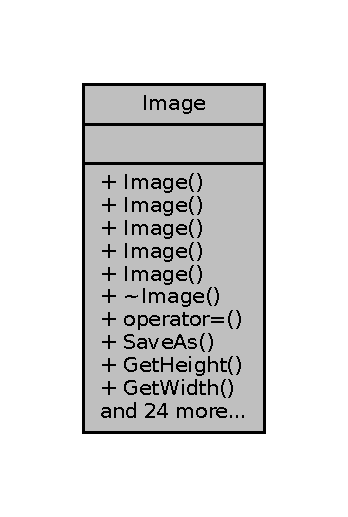
\includegraphics[width=167pt]{classImage__coll__graph}
\end{center}
\end{figure}
\subsection*{Public Member Functions}
\begin{DoxyCompactItemize}
\item 
\mbox{\Hypertarget{classImage_a58edd1c45b4faeb5f789b0d036d02313}\label{classImage_a58edd1c45b4faeb5f789b0d036d02313}} 
\hyperlink{classImage_a58edd1c45b4faeb5f789b0d036d02313}{Image} ()
\begin{DoxyCompactList}\small\item\em Default constructor accepting no parameters. \end{DoxyCompactList}\item 
\hyperlink{classImage_a05c964ca59502cc32c30e8ab89b5e920}{Image} (int w, int h)
\begin{DoxyCompactList}\small\item\em Creates a \char`\"{}blank\char`\"{} image of a given width and height. \end{DoxyCompactList}\item 
\hyperlink{classImage_a81e88caba6ef6c0ed639bf1f25e9d441}{Image} (const std\+::string \&filename)
\begin{DoxyCompactList}\small\item\em Load an image from the hard drive given the filename passed. \end{DoxyCompactList}\item 
\mbox{\Hypertarget{classImage_a7f515a9c20a88c2010a5ace21c263925}\label{classImage_a7f515a9c20a88c2010a5ace21c263925}} 
{\bfseries Image} (const unsigned char $\ast$data, int length)
\item 
\hyperlink{classImage_a34410a36b132ab597a8878d45facc89a}{Image} (const \hyperlink{classImage}{Image} \&image)
\begin{DoxyCompactList}\small\item\em A copy constructor that allows to copy/duplicate any \hyperlink{classImage}{Image}. \end{DoxyCompactList}\item 
\mbox{\Hypertarget{classImage_a0294f63700543e11c0f0da85601c7ae5}\label{classImage_a0294f63700543e11c0f0da85601c7ae5}} 
\hyperlink{classImage_a0294f63700543e11c0f0da85601c7ae5}{$\sim$\+Image} ()
\begin{DoxyCompactList}\small\item\em A destructor. \end{DoxyCompactList}\item 
void \hyperlink{classImage_ae6b1cdd82584ce9fb729c1e062ee088b}{operator=} (const \hyperlink{classImage}{Image} \&image)
\begin{DoxyCompactList}\small\item\em Deep copy an image passed in as parameter into another object. \end{DoxyCompactList}\item 
void \hyperlink{classImage_afd027f3a969d6ff41c76a4ab2599d85d}{Save\+As} (const std\+::string \&filename)
\begin{DoxyCompactList}\small\item\em A method that takes in a string (or character array) and saves the \hyperlink{classImage}{Image} object into a P\+NG image. \end{DoxyCompactList}\item 
int \hyperlink{classImage_a631ead4be012caf49b3209d2ac401214}{Get\+Height} () const
\item 
int \hyperlink{classImage_a3da5012d5e314ce03b53d77276232186}{Get\+Width} () const
\item 
int \hyperlink{classImage_a8ee1acb5476bf0fecac66f5dfdd47a38}{Get\+Size} () const
\item 
float \hyperlink{classImage_a9efc74ed4a9af25d1eb01416ec47e78e}{Get\+Max\+Float\+Val} () const
\item 
int \hyperlink{classImage_aec11158c35b24ba60a835c877d791b36}{Get\+Component\+Num} () const
\item 
\hyperlink{classColor}{Color} $\ast$ \hyperlink{classImage_a01fc9742fb7bb83f66027d5c9091d477}{Get\+Pixel} (int x, int y) const
\item 
\hyperlink{classColor}{Color} $\ast$ \hyperlink{classImage_a1d2472f49fc5cd5458f32fc54affddcf}{Get\+Pixel} (int i) const
\item 
void \hyperlink{classImage_a4b464d4f6348e8be2480688d9871ceac}{Set\+Pixel} (int x, int y, const \hyperlink{classColor}{Color} \&pixel)
\begin{DoxyCompactList}\small\item\em Sets the \hyperlink{classColor}{Color} pixel at the width and height passed as parameter to a new \hyperlink{classColor}{Color} object passed as parameter. \end{DoxyCompactList}\item 
void \hyperlink{classImage_a9774c194cd627ccb7dfe4165e7e5e996}{Set\+Pixel} (int i, const \hyperlink{classColor}{Color} \&pixel)
\begin{DoxyCompactList}\small\item\em Sets the \hyperlink{classColor}{Color} pixel at the index passeed as parameter to a new \hyperlink{classColor}{Color} object also passed as a parameter. \end{DoxyCompactList}\item 
\mbox{\Hypertarget{classImage_a58edd1c45b4faeb5f789b0d036d02313}\label{classImage_a58edd1c45b4faeb5f789b0d036d02313}} 
\hyperlink{classImage_a58edd1c45b4faeb5f789b0d036d02313}{Image} ()
\begin{DoxyCompactList}\small\item\em Default constructor accepting no parameters. \end{DoxyCompactList}\item 
\hyperlink{classImage_a05c964ca59502cc32c30e8ab89b5e920}{Image} (int w, int h)
\begin{DoxyCompactList}\small\item\em Creates a \char`\"{}blank\char`\"{} image of a given width and height. \end{DoxyCompactList}\item 
\hyperlink{classImage_a81e88caba6ef6c0ed639bf1f25e9d441}{Image} (const std\+::string \&filename)
\begin{DoxyCompactList}\small\item\em Load an image from the hard drive given the filename passed. \end{DoxyCompactList}\item 
\mbox{\Hypertarget{classImage_a7f515a9c20a88c2010a5ace21c263925}\label{classImage_a7f515a9c20a88c2010a5ace21c263925}} 
{\bfseries Image} (const unsigned char $\ast$data, int length)
\item 
\hyperlink{classImage_a34410a36b132ab597a8878d45facc89a}{Image} (const \hyperlink{classImage}{Image} \&image)
\begin{DoxyCompactList}\small\item\em A copy constructor that allows to copy/duplicate any \hyperlink{classImage}{Image}. \end{DoxyCompactList}\item 
\mbox{\Hypertarget{classImage_a0294f63700543e11c0f0da85601c7ae5}\label{classImage_a0294f63700543e11c0f0da85601c7ae5}} 
\hyperlink{classImage_a0294f63700543e11c0f0da85601c7ae5}{$\sim$\+Image} ()
\begin{DoxyCompactList}\small\item\em A destructor. \end{DoxyCompactList}\item 
void \hyperlink{classImage_ae6b1cdd82584ce9fb729c1e062ee088b}{operator=} (const \hyperlink{classImage}{Image} \&image)
\begin{DoxyCompactList}\small\item\em Deep copy an image passed in as parameter into another object. \end{DoxyCompactList}\item 
void \hyperlink{classImage_afd027f3a969d6ff41c76a4ab2599d85d}{Save\+As} (const std\+::string \&filename)
\begin{DoxyCompactList}\small\item\em A method that takes in a string (or character array) and saves the \hyperlink{classImage}{Image} object into a P\+NG image. \end{DoxyCompactList}\item 
int \hyperlink{classImage_a631ead4be012caf49b3209d2ac401214}{Get\+Height} () const
\item 
int \hyperlink{classImage_a3da5012d5e314ce03b53d77276232186}{Get\+Width} () const
\item 
int \hyperlink{classImage_a8ee1acb5476bf0fecac66f5dfdd47a38}{Get\+Size} () const
\item 
float \hyperlink{classImage_a9efc74ed4a9af25d1eb01416ec47e78e}{Get\+Max\+Float\+Val} () const
\item 
int \hyperlink{classImage_aec11158c35b24ba60a835c877d791b36}{Get\+Component\+Num} () const
\item 
\hyperlink{classColor}{Color} $\ast$ \hyperlink{classImage_ae7136a83009449a0238f03efa1027c68}{Get\+Pixel} (int x, int y) const
\item 
\hyperlink{classColor}{Color} $\ast$ \hyperlink{classImage_aa54365cbbea7a483c275e8898b1ed119}{Get\+Pixel} (int i) const
\item 
void \hyperlink{classImage_a4b464d4f6348e8be2480688d9871ceac}{Set\+Pixel} (int x, int y, const \hyperlink{classColor}{Color} \&pixel)
\begin{DoxyCompactList}\small\item\em Sets the \hyperlink{classColor}{Color} pixel at the width and height passed as parameter to a new \hyperlink{classColor}{Color} object passed as parameter. \end{DoxyCompactList}\item 
void \hyperlink{classImage_a9774c194cd627ccb7dfe4165e7e5e996}{Set\+Pixel} (int i, const \hyperlink{classColor}{Color} \&pixel)
\begin{DoxyCompactList}\small\item\em Sets the \hyperlink{classColor}{Color} pixel at the index passeed as parameter to a new \hyperlink{classColor}{Color} object also passed as a parameter. \end{DoxyCompactList}\end{DoxyCompactItemize}


\subsection{Detailed Description}
A class that holds content representing a P\+NG image. 

\subsection{Constructor \& Destructor Documentation}
\mbox{\Hypertarget{classImage_a05c964ca59502cc32c30e8ab89b5e920}\label{classImage_a05c964ca59502cc32c30e8ab89b5e920}} 
\index{Image@{Image}!Image@{Image}}
\index{Image@{Image}!Image@{Image}}
\subsubsection{\texorpdfstring{Image()}{Image()}\hspace{0.1cm}{\footnotesize\ttfamily [1/6]}}
{\footnotesize\ttfamily Image\+::\+Image (\begin{DoxyParamCaption}\item[{int}]{w,  }\item[{int}]{h }\end{DoxyParamCaption})}



Creates a \char`\"{}blank\char`\"{} image of a given width and height. 


\begin{DoxyParams}[1]{Parameters}
\mbox{\tt in}  & {\em w} & An integer representing the width of the image to be created. \\
\hline
\mbox{\tt in}  & {\em h} & An integer representing the height of the image to be created. \\
\hline
\end{DoxyParams}
\mbox{\Hypertarget{classImage_a81e88caba6ef6c0ed639bf1f25e9d441}\label{classImage_a81e88caba6ef6c0ed639bf1f25e9d441}} 
\index{Image@{Image}!Image@{Image}}
\index{Image@{Image}!Image@{Image}}
\subsubsection{\texorpdfstring{Image()}{Image()}\hspace{0.1cm}{\footnotesize\ttfamily [2/6]}}
{\footnotesize\ttfamily Image\+::\+Image (\begin{DoxyParamCaption}\item[{const std\+::string \&}]{filename }\end{DoxyParamCaption})}



Load an image from the hard drive given the filename passed. 


\begin{DoxyParams}[1]{Parameters}
\mbox{\tt in}  & {\em filename} & A string representing the relative location of the image. \\
\hline
\end{DoxyParams}
\mbox{\Hypertarget{classImage_a34410a36b132ab597a8878d45facc89a}\label{classImage_a34410a36b132ab597a8878d45facc89a}} 
\index{Image@{Image}!Image@{Image}}
\index{Image@{Image}!Image@{Image}}
\subsubsection{\texorpdfstring{Image()}{Image()}\hspace{0.1cm}{\footnotesize\ttfamily [3/6]}}
{\footnotesize\ttfamily Image\+::\+Image (\begin{DoxyParamCaption}\item[{const \hyperlink{classImage}{Image} \&}]{image }\end{DoxyParamCaption})}



A copy constructor that allows to copy/duplicate any \hyperlink{classImage}{Image}. 


\begin{DoxyParams}[1]{Parameters}
\mbox{\tt in}  & {\em image} & An \hyperlink{classImage}{Image} object used to make a duplicate of. \\
\hline
\end{DoxyParams}
\mbox{\Hypertarget{classImage_a05c964ca59502cc32c30e8ab89b5e920}\label{classImage_a05c964ca59502cc32c30e8ab89b5e920}} 
\index{Image@{Image}!Image@{Image}}
\index{Image@{Image}!Image@{Image}}
\subsubsection{\texorpdfstring{Image()}{Image()}\hspace{0.1cm}{\footnotesize\ttfamily [4/6]}}
{\footnotesize\ttfamily Image\+::\+Image (\begin{DoxyParamCaption}\item[{int}]{w,  }\item[{int}]{h }\end{DoxyParamCaption})}



Creates a \char`\"{}blank\char`\"{} image of a given width and height. 


\begin{DoxyParams}[1]{Parameters}
\mbox{\tt in}  & {\em w} & An integer representing the width of the image to be created. \\
\hline
\mbox{\tt in}  & {\em h} & An integer representing the height of the image to be created. \\
\hline
\end{DoxyParams}
\mbox{\Hypertarget{classImage_a81e88caba6ef6c0ed639bf1f25e9d441}\label{classImage_a81e88caba6ef6c0ed639bf1f25e9d441}} 
\index{Image@{Image}!Image@{Image}}
\index{Image@{Image}!Image@{Image}}
\subsubsection{\texorpdfstring{Image()}{Image()}\hspace{0.1cm}{\footnotesize\ttfamily [5/6]}}
{\footnotesize\ttfamily Image\+::\+Image (\begin{DoxyParamCaption}\item[{const std\+::string \&}]{filename }\end{DoxyParamCaption})}



Load an image from the hard drive given the filename passed. 


\begin{DoxyParams}[1]{Parameters}
\mbox{\tt in}  & {\em filename} & A string representing the relative location of the image. \\
\hline
\end{DoxyParams}
\mbox{\Hypertarget{classImage_a34410a36b132ab597a8878d45facc89a}\label{classImage_a34410a36b132ab597a8878d45facc89a}} 
\index{Image@{Image}!Image@{Image}}
\index{Image@{Image}!Image@{Image}}
\subsubsection{\texorpdfstring{Image()}{Image()}\hspace{0.1cm}{\footnotesize\ttfamily [6/6]}}
{\footnotesize\ttfamily Image\+::\+Image (\begin{DoxyParamCaption}\item[{const \hyperlink{classImage}{Image} \&}]{image }\end{DoxyParamCaption})}



A copy constructor that allows to copy/duplicate any \hyperlink{classImage}{Image}. 


\begin{DoxyParams}[1]{Parameters}
\mbox{\tt in}  & {\em image} & An \hyperlink{classImage}{Image} object used to make a duplicate of. \\
\hline
\end{DoxyParams}


\subsection{Member Function Documentation}
\mbox{\Hypertarget{classImage_aec11158c35b24ba60a835c877d791b36}\label{classImage_aec11158c35b24ba60a835c877d791b36}} 
\index{Image@{Image}!Get\+Component\+Num@{Get\+Component\+Num}}
\index{Get\+Component\+Num@{Get\+Component\+Num}!Image@{Image}}
\subsubsection{\texorpdfstring{Get\+Component\+Num()}{GetComponentNum()}\hspace{0.1cm}{\footnotesize\ttfamily [1/2]}}
{\footnotesize\ttfamily int Image\+::\+Get\+Component\+Num (\begin{DoxyParamCaption}{ }\end{DoxyParamCaption}) const}

\begin{DoxyReturn}{Returns}
The number of components each pixel has. 
\end{DoxyReturn}
\mbox{\Hypertarget{classImage_aec11158c35b24ba60a835c877d791b36}\label{classImage_aec11158c35b24ba60a835c877d791b36}} 
\index{Image@{Image}!Get\+Component\+Num@{Get\+Component\+Num}}
\index{Get\+Component\+Num@{Get\+Component\+Num}!Image@{Image}}
\subsubsection{\texorpdfstring{Get\+Component\+Num()}{GetComponentNum()}\hspace{0.1cm}{\footnotesize\ttfamily [2/2]}}
{\footnotesize\ttfamily int Image\+::\+Get\+Component\+Num (\begin{DoxyParamCaption}{ }\end{DoxyParamCaption}) const}

\begin{DoxyReturn}{Returns}
The number of components each pixel has. 
\end{DoxyReturn}
\mbox{\Hypertarget{classImage_a631ead4be012caf49b3209d2ac401214}\label{classImage_a631ead4be012caf49b3209d2ac401214}} 
\index{Image@{Image}!Get\+Height@{Get\+Height}}
\index{Get\+Height@{Get\+Height}!Image@{Image}}
\subsubsection{\texorpdfstring{Get\+Height()}{GetHeight()}\hspace{0.1cm}{\footnotesize\ttfamily [1/2]}}
{\footnotesize\ttfamily int Image\+::\+Get\+Height (\begin{DoxyParamCaption}{ }\end{DoxyParamCaption}) const}

\begin{DoxyReturn}{Returns}
The height of the image object. 
\end{DoxyReturn}
\mbox{\Hypertarget{classImage_a631ead4be012caf49b3209d2ac401214}\label{classImage_a631ead4be012caf49b3209d2ac401214}} 
\index{Image@{Image}!Get\+Height@{Get\+Height}}
\index{Get\+Height@{Get\+Height}!Image@{Image}}
\subsubsection{\texorpdfstring{Get\+Height()}{GetHeight()}\hspace{0.1cm}{\footnotesize\ttfamily [2/2]}}
{\footnotesize\ttfamily int Image\+::\+Get\+Height (\begin{DoxyParamCaption}{ }\end{DoxyParamCaption}) const}

\begin{DoxyReturn}{Returns}
The height of the image object. 
\end{DoxyReturn}
\mbox{\Hypertarget{classImage_a9efc74ed4a9af25d1eb01416ec47e78e}\label{classImage_a9efc74ed4a9af25d1eb01416ec47e78e}} 
\index{Image@{Image}!Get\+Max\+Float\+Val@{Get\+Max\+Float\+Val}}
\index{Get\+Max\+Float\+Val@{Get\+Max\+Float\+Val}!Image@{Image}}
\subsubsection{\texorpdfstring{Get\+Max\+Float\+Val()}{GetMaxFloatVal()}\hspace{0.1cm}{\footnotesize\ttfamily [1/2]}}
{\footnotesize\ttfamily float Image\+::\+Get\+Max\+Float\+Val (\begin{DoxyParamCaption}{ }\end{DoxyParamCaption}) const}

\begin{DoxyReturn}{Returns}
The max r,g, or b that is found in the image. 
\end{DoxyReturn}
\mbox{\Hypertarget{classImage_a9efc74ed4a9af25d1eb01416ec47e78e}\label{classImage_a9efc74ed4a9af25d1eb01416ec47e78e}} 
\index{Image@{Image}!Get\+Max\+Float\+Val@{Get\+Max\+Float\+Val}}
\index{Get\+Max\+Float\+Val@{Get\+Max\+Float\+Val}!Image@{Image}}
\subsubsection{\texorpdfstring{Get\+Max\+Float\+Val()}{GetMaxFloatVal()}\hspace{0.1cm}{\footnotesize\ttfamily [2/2]}}
{\footnotesize\ttfamily float Image\+::\+Get\+Max\+Float\+Val (\begin{DoxyParamCaption}{ }\end{DoxyParamCaption}) const}

\begin{DoxyReturn}{Returns}
The max r,g, or b that is found in the image. 
\end{DoxyReturn}
for each pixel in each original picture \mbox{\Hypertarget{classImage_a01fc9742fb7bb83f66027d5c9091d477}\label{classImage_a01fc9742fb7bb83f66027d5c9091d477}} 
\index{Image@{Image}!Get\+Pixel@{Get\+Pixel}}
\index{Get\+Pixel@{Get\+Pixel}!Image@{Image}}
\subsubsection{\texorpdfstring{Get\+Pixel()}{GetPixel()}\hspace{0.1cm}{\footnotesize\ttfamily [1/4]}}
{\footnotesize\ttfamily \hyperlink{classColor}{Color} $\ast$ Image\+::\+Get\+Pixel (\begin{DoxyParamCaption}\item[{int}]{x,  }\item[{int}]{y }\end{DoxyParamCaption}) const}


\begin{DoxyParams}[1]{Parameters}
\mbox{\tt in}  & {\em x} & An integer representing the x-\/position of the pixel to return. \\
\hline
\mbox{\tt in}  & {\em y} & An integer representing the y-\/position of the pixel to return.\\
\hline
\end{DoxyParams}
\begin{DoxyReturn}{Returns}
A \hyperlink{classColor}{Color} object pointer, pointing to the \hyperlink{classColor}{Color} at the width and height passed in as parameters. 
\end{DoxyReturn}
\mbox{\Hypertarget{classImage_ae7136a83009449a0238f03efa1027c68}\label{classImage_ae7136a83009449a0238f03efa1027c68}} 
\index{Image@{Image}!Get\+Pixel@{Get\+Pixel}}
\index{Get\+Pixel@{Get\+Pixel}!Image@{Image}}
\subsubsection{\texorpdfstring{Get\+Pixel()}{GetPixel()}\hspace{0.1cm}{\footnotesize\ttfamily [2/4]}}
{\footnotesize\ttfamily \hyperlink{classColor}{Color}$\ast$ Image\+::\+Get\+Pixel (\begin{DoxyParamCaption}\item[{int}]{x,  }\item[{int}]{y }\end{DoxyParamCaption}) const}


\begin{DoxyParams}[1]{Parameters}
\mbox{\tt in}  & {\em x} & An integer representing the x-\/position of the pixel to return. \\
\hline
\mbox{\tt in}  & {\em y} & An integer representing the y-\/position of the pixel to return.\\
\hline
\end{DoxyParams}
\begin{DoxyReturn}{Returns}
A \hyperlink{classColor}{Color} object pointer, pointing to the \hyperlink{classColor}{Color} at the width and height passed in as parameters. 
\end{DoxyReturn}
\mbox{\Hypertarget{classImage_a1d2472f49fc5cd5458f32fc54affddcf}\label{classImage_a1d2472f49fc5cd5458f32fc54affddcf}} 
\index{Image@{Image}!Get\+Pixel@{Get\+Pixel}}
\index{Get\+Pixel@{Get\+Pixel}!Image@{Image}}
\subsubsection{\texorpdfstring{Get\+Pixel()}{GetPixel()}\hspace{0.1cm}{\footnotesize\ttfamily [3/4]}}
{\footnotesize\ttfamily \hyperlink{classColor}{Color} $\ast$ Image\+::\+Get\+Pixel (\begin{DoxyParamCaption}\item[{int}]{i }\end{DoxyParamCaption}) const}


\begin{DoxyParams}[1]{Parameters}
\mbox{\tt in}  & {\em i} & integer representing where the image color to retrive is situated\\
\hline
\end{DoxyParams}
\begin{DoxyReturn}{Returns}
\hyperlink{classColor}{Color} object pointer, pointing to the \hyperlink{classColor}{Color} at the given index in the image. 
\end{DoxyReturn}
\mbox{\Hypertarget{classImage_aa54365cbbea7a483c275e8898b1ed119}\label{classImage_aa54365cbbea7a483c275e8898b1ed119}} 
\index{Image@{Image}!Get\+Pixel@{Get\+Pixel}}
\index{Get\+Pixel@{Get\+Pixel}!Image@{Image}}
\subsubsection{\texorpdfstring{Get\+Pixel()}{GetPixel()}\hspace{0.1cm}{\footnotesize\ttfamily [4/4]}}
{\footnotesize\ttfamily \hyperlink{classColor}{Color}$\ast$ Image\+::\+Get\+Pixel (\begin{DoxyParamCaption}\item[{int}]{i }\end{DoxyParamCaption}) const}


\begin{DoxyParams}[1]{Parameters}
\mbox{\tt in}  & {\em i} & integer representing where the image color to retrive is situated\\
\hline
\end{DoxyParams}
\begin{DoxyReturn}{Returns}
\hyperlink{classColor}{Color} object pointer, pointing to the \hyperlink{classColor}{Color} at the given index in the image. 
\end{DoxyReturn}
\mbox{\Hypertarget{classImage_a8ee1acb5476bf0fecac66f5dfdd47a38}\label{classImage_a8ee1acb5476bf0fecac66f5dfdd47a38}} 
\index{Image@{Image}!Get\+Size@{Get\+Size}}
\index{Get\+Size@{Get\+Size}!Image@{Image}}
\subsubsection{\texorpdfstring{Get\+Size()}{GetSize()}\hspace{0.1cm}{\footnotesize\ttfamily [1/2]}}
{\footnotesize\ttfamily int Image\+::\+Get\+Size (\begin{DoxyParamCaption}{ }\end{DoxyParamCaption}) const}

\begin{DoxyReturn}{Returns}
The total number of pixels of the image object. 
\end{DoxyReturn}
\mbox{\Hypertarget{classImage_a8ee1acb5476bf0fecac66f5dfdd47a38}\label{classImage_a8ee1acb5476bf0fecac66f5dfdd47a38}} 
\index{Image@{Image}!Get\+Size@{Get\+Size}}
\index{Get\+Size@{Get\+Size}!Image@{Image}}
\subsubsection{\texorpdfstring{Get\+Size()}{GetSize()}\hspace{0.1cm}{\footnotesize\ttfamily [2/2]}}
{\footnotesize\ttfamily int Image\+::\+Get\+Size (\begin{DoxyParamCaption}{ }\end{DoxyParamCaption}) const}

\begin{DoxyReturn}{Returns}
The total number of pixels of the image object. 
\end{DoxyReturn}
\mbox{\Hypertarget{classImage_a3da5012d5e314ce03b53d77276232186}\label{classImage_a3da5012d5e314ce03b53d77276232186}} 
\index{Image@{Image}!Get\+Width@{Get\+Width}}
\index{Get\+Width@{Get\+Width}!Image@{Image}}
\subsubsection{\texorpdfstring{Get\+Width()}{GetWidth()}\hspace{0.1cm}{\footnotesize\ttfamily [1/2]}}
{\footnotesize\ttfamily int Image\+::\+Get\+Width (\begin{DoxyParamCaption}{ }\end{DoxyParamCaption}) const}

\begin{DoxyReturn}{Returns}
The width of the image object. 
\end{DoxyReturn}
\mbox{\Hypertarget{classImage_a3da5012d5e314ce03b53d77276232186}\label{classImage_a3da5012d5e314ce03b53d77276232186}} 
\index{Image@{Image}!Get\+Width@{Get\+Width}}
\index{Get\+Width@{Get\+Width}!Image@{Image}}
\subsubsection{\texorpdfstring{Get\+Width()}{GetWidth()}\hspace{0.1cm}{\footnotesize\ttfamily [2/2]}}
{\footnotesize\ttfamily int Image\+::\+Get\+Width (\begin{DoxyParamCaption}{ }\end{DoxyParamCaption}) const}

\begin{DoxyReturn}{Returns}
The width of the image object. 
\end{DoxyReturn}
\mbox{\Hypertarget{classImage_ae6b1cdd82584ce9fb729c1e062ee088b}\label{classImage_ae6b1cdd82584ce9fb729c1e062ee088b}} 
\index{Image@{Image}!operator=@{operator=}}
\index{operator=@{operator=}!Image@{Image}}
\subsubsection{\texorpdfstring{operator=()}{operator=()}\hspace{0.1cm}{\footnotesize\ttfamily [1/2]}}
{\footnotesize\ttfamily void Image\+::operator= (\begin{DoxyParamCaption}\item[{const \hyperlink{classImage}{Image} \&}]{image }\end{DoxyParamCaption})}



Deep copy an image passed in as parameter into another object. 


\begin{DoxyParams}[1]{Parameters}
\mbox{\tt in}  & {\em image} & An \hyperlink{classImage}{Image} object used to make a duplicate of. \\
\hline
\end{DoxyParams}
\mbox{\Hypertarget{classImage_ae6b1cdd82584ce9fb729c1e062ee088b}\label{classImage_ae6b1cdd82584ce9fb729c1e062ee088b}} 
\index{Image@{Image}!operator=@{operator=}}
\index{operator=@{operator=}!Image@{Image}}
\subsubsection{\texorpdfstring{operator=()}{operator=()}\hspace{0.1cm}{\footnotesize\ttfamily [2/2]}}
{\footnotesize\ttfamily void Image\+::operator= (\begin{DoxyParamCaption}\item[{const \hyperlink{classImage}{Image} \&}]{image }\end{DoxyParamCaption})}



Deep copy an image passed in as parameter into another object. 


\begin{DoxyParams}[1]{Parameters}
\mbox{\tt in}  & {\em image} & An \hyperlink{classImage}{Image} object used to make a duplicate of. \\
\hline
\end{DoxyParams}
\mbox{\Hypertarget{classImage_afd027f3a969d6ff41c76a4ab2599d85d}\label{classImage_afd027f3a969d6ff41c76a4ab2599d85d}} 
\index{Image@{Image}!Save\+As@{Save\+As}}
\index{Save\+As@{Save\+As}!Image@{Image}}
\subsubsection{\texorpdfstring{Save\+As()}{SaveAs()}\hspace{0.1cm}{\footnotesize\ttfamily [1/2]}}
{\footnotesize\ttfamily void Image\+::\+Save\+As (\begin{DoxyParamCaption}\item[{const std\+::string \&}]{filename }\end{DoxyParamCaption})}



A method that takes in a string (or character array) and saves the \hyperlink{classImage}{Image} object into a P\+NG image. 


\begin{DoxyParams}[1]{Parameters}
\mbox{\tt in}  & {\em filename} & A string representing the name and location of the \hyperlink{classImage}{Image} being saved. \\
\hline
\end{DoxyParams}
\mbox{\Hypertarget{classImage_afd027f3a969d6ff41c76a4ab2599d85d}\label{classImage_afd027f3a969d6ff41c76a4ab2599d85d}} 
\index{Image@{Image}!Save\+As@{Save\+As}}
\index{Save\+As@{Save\+As}!Image@{Image}}
\subsubsection{\texorpdfstring{Save\+As()}{SaveAs()}\hspace{0.1cm}{\footnotesize\ttfamily [2/2]}}
{\footnotesize\ttfamily void Image\+::\+Save\+As (\begin{DoxyParamCaption}\item[{const std\+::string \&}]{filename }\end{DoxyParamCaption})}



A method that takes in a string (or character array) and saves the \hyperlink{classImage}{Image} object into a P\+NG image. 


\begin{DoxyParams}[1]{Parameters}
\mbox{\tt in}  & {\em filename} & A string representing the name and location of the \hyperlink{classImage}{Image} being saved. \\
\hline
\end{DoxyParams}
\mbox{\Hypertarget{classImage_a4b464d4f6348e8be2480688d9871ceac}\label{classImage_a4b464d4f6348e8be2480688d9871ceac}} 
\index{Image@{Image}!Set\+Pixel@{Set\+Pixel}}
\index{Set\+Pixel@{Set\+Pixel}!Image@{Image}}
\subsubsection{\texorpdfstring{Set\+Pixel()}{SetPixel()}\hspace{0.1cm}{\footnotesize\ttfamily [1/4]}}
{\footnotesize\ttfamily void Image\+::\+Set\+Pixel (\begin{DoxyParamCaption}\item[{int}]{x,  }\item[{int}]{y,  }\item[{const \hyperlink{classColor}{Color} \&}]{pixel }\end{DoxyParamCaption})}



Sets the \hyperlink{classColor}{Color} pixel at the width and height passed as parameter to a new \hyperlink{classColor}{Color} object passed as parameter. 


\begin{DoxyParams}[1]{Parameters}
\mbox{\tt in}  & {\em x} & An integer representing the x-\/position of the pixel to return. \\
\hline
\mbox{\tt in}  & {\em y} & An integer representing the y-\/position of the pixel to return. \\
\hline
\mbox{\tt in}  & {\em pixel} & A \hyperlink{classColor}{Color} object to be used as new color of pixel at (x,y). \\
\hline
\end{DoxyParams}
\mbox{\Hypertarget{classImage_a4b464d4f6348e8be2480688d9871ceac}\label{classImage_a4b464d4f6348e8be2480688d9871ceac}} 
\index{Image@{Image}!Set\+Pixel@{Set\+Pixel}}
\index{Set\+Pixel@{Set\+Pixel}!Image@{Image}}
\subsubsection{\texorpdfstring{Set\+Pixel()}{SetPixel()}\hspace{0.1cm}{\footnotesize\ttfamily [2/4]}}
{\footnotesize\ttfamily void Image\+::\+Set\+Pixel (\begin{DoxyParamCaption}\item[{int}]{x,  }\item[{int}]{y,  }\item[{const \hyperlink{classColor}{Color} \&}]{pixel }\end{DoxyParamCaption})}



Sets the \hyperlink{classColor}{Color} pixel at the width and height passed as parameter to a new \hyperlink{classColor}{Color} object passed as parameter. 


\begin{DoxyParams}[1]{Parameters}
\mbox{\tt in}  & {\em x} & An integer representing the x-\/position of the pixel to return. \\
\hline
\mbox{\tt in}  & {\em y} & An integer representing the y-\/position of the pixel to return. \\
\hline
\mbox{\tt in}  & {\em pixel} & A \hyperlink{classColor}{Color} object to be used as new color of pixel at (x,y). \\
\hline
\end{DoxyParams}
\mbox{\Hypertarget{classImage_a9774c194cd627ccb7dfe4165e7e5e996}\label{classImage_a9774c194cd627ccb7dfe4165e7e5e996}} 
\index{Image@{Image}!Set\+Pixel@{Set\+Pixel}}
\index{Set\+Pixel@{Set\+Pixel}!Image@{Image}}
\subsubsection{\texorpdfstring{Set\+Pixel()}{SetPixel()}\hspace{0.1cm}{\footnotesize\ttfamily [3/4]}}
{\footnotesize\ttfamily void Image\+::\+Set\+Pixel (\begin{DoxyParamCaption}\item[{int}]{i,  }\item[{const \hyperlink{classColor}{Color} \&}]{pixel }\end{DoxyParamCaption})}



Sets the \hyperlink{classColor}{Color} pixel at the index passeed as parameter to a new \hyperlink{classColor}{Color} object also passed as a parameter. 


\begin{DoxyParams}[1]{Parameters}
\mbox{\tt in}  & {\em i} & An integer representing where the image color to change is located. \\
\hline
\mbox{\tt in}  & {\em pixel} & A \hyperlink{classColor}{Color} object to be used as new color of pixel at (x,y). \\
\hline
\end{DoxyParams}
\mbox{\Hypertarget{classImage_a9774c194cd627ccb7dfe4165e7e5e996}\label{classImage_a9774c194cd627ccb7dfe4165e7e5e996}} 
\index{Image@{Image}!Set\+Pixel@{Set\+Pixel}}
\index{Set\+Pixel@{Set\+Pixel}!Image@{Image}}
\subsubsection{\texorpdfstring{Set\+Pixel()}{SetPixel()}\hspace{0.1cm}{\footnotesize\ttfamily [4/4]}}
{\footnotesize\ttfamily void Image\+::\+Set\+Pixel (\begin{DoxyParamCaption}\item[{int}]{i,  }\item[{const \hyperlink{classColor}{Color} \&}]{pixel }\end{DoxyParamCaption})}



Sets the \hyperlink{classColor}{Color} pixel at the index passeed as parameter to a new \hyperlink{classColor}{Color} object also passed as a parameter. 


\begin{DoxyParams}[1]{Parameters}
\mbox{\tt in}  & {\em i} & An integer representing where the image color to change is located. \\
\hline
\mbox{\tt in}  & {\em pixel} & A \hyperlink{classColor}{Color} object to be used as new color of pixel at (x,y). \\
\hline
\end{DoxyParams}


The documentation for this class was generated from the following files\+:\begin{DoxyCompactItemize}
\item 
/home/user/repo/project/src/\+Image\+Processing/image.\+h\item 
/home/user/repo/project/src/\+Image\+Processing/image.\+cc\end{DoxyCompactItemize}

\hypertarget{classImageProcessor}{}\section{Image\+Processor Class Reference}
\label{classImageProcessor}\index{Image\+Processor@{Image\+Processor}}


A class that applies any filter.  




{\ttfamily \#include $<$image\+\_\+processor.\+h$>$}



Collaboration diagram for Image\+Processor\+:\nopagebreak
\begin{figure}[H]
\begin{center}
\leavevmode
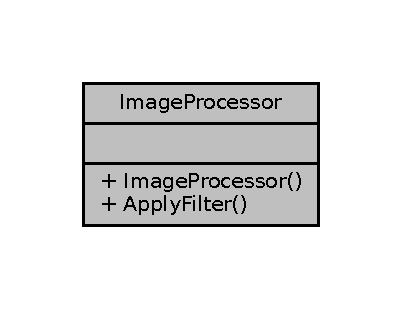
\includegraphics[width=193pt]{classImageProcessor__coll__graph}
\end{center}
\end{figure}
\subsection*{Public Member Functions}
\begin{DoxyCompactItemize}
\item 
\mbox{\Hypertarget{classImageProcessor_aa9201a4d14b20ac968919145db3a588b}\label{classImageProcessor_aa9201a4d14b20ac968919145db3a588b}} 
\hyperlink{classImageProcessor_aa9201a4d14b20ac968919145db3a588b}{Image\+Processor} ()
\begin{DoxyCompactList}\small\item\em Constructor that defines the map of filters. \end{DoxyCompactList}\item 
void \hyperlink{classImageProcessor_ad7ed2647ee8a70d015216d8883e25804}{Apply\+Filter} (const std\+::string \&input\+File, const std\+::string \&output\+File, const std\+::string \&filter\+Type)
\begin{DoxyCompactList}\small\item\em Applies a filter to an \hyperlink{classImage}{Image} and saves solution into another file. \end{DoxyCompactList}\end{DoxyCompactItemize}


\subsection{Detailed Description}
A class that applies any filter. 

\subsection{Member Function Documentation}
\mbox{\Hypertarget{classImageProcessor_ad7ed2647ee8a70d015216d8883e25804}\label{classImageProcessor_ad7ed2647ee8a70d015216d8883e25804}} 
\index{Image\+Processor@{Image\+Processor}!Apply\+Filter@{Apply\+Filter}}
\index{Apply\+Filter@{Apply\+Filter}!Image\+Processor@{Image\+Processor}}
\subsubsection{\texorpdfstring{Apply\+Filter()}{ApplyFilter()}}
{\footnotesize\ttfamily void Image\+Processor\+::\+Apply\+Filter (\begin{DoxyParamCaption}\item[{const std\+::string \&}]{input\+File,  }\item[{const std\+::string \&}]{output\+File,  }\item[{const std\+::string \&}]{filter\+Type }\end{DoxyParamCaption})}



Applies a filter to an \hyperlink{classImage}{Image} and saves solution into another file. 


\begin{DoxyParams}[1]{Parameters}
\mbox{\tt in}  & {\em input\+File} & A filename of the image to apply filter to. \\
\hline
\mbox{\tt in}  & {\em output\+File} & A filename of where the filtered image should be saved. \\
\hline
\mbox{\tt in}  & {\em filter\+Type} & A filtertype that should be applied. \\
\hline
\end{DoxyParams}


The documentation for this class was generated from the following files\+:\begin{DoxyCompactItemize}
\item 
/home/user/repo/project/\+Image\+Processing/\hyperlink{image__processor_8h}{image\+\_\+processor.\+h}\item 
/home/user/repo/project/\+Image\+Processing/\hyperlink{image__processor_8cc}{image\+\_\+processor.\+cc}\end{DoxyCompactItemize}

\hypertarget{classIMovement}{}\section{I\+Movement Class Reference}
\label{classIMovement}\index{I\+Movement@{I\+Movement}}


An Interface for any Movement Strategy.  




{\ttfamily \#include $<$I\+Movement.\+h$>$}



Inheritance diagram for I\+Movement\+:\nopagebreak
\begin{figure}[H]
\begin{center}
\leavevmode
\includegraphics[width=234pt]{classIMovement__inherit__graph}
\end{center}
\end{figure}


Collaboration diagram for I\+Movement\+:\nopagebreak
\begin{figure}[H]
\begin{center}
\leavevmode
\includegraphics[width=151pt]{classIMovement__coll__graph}
\end{center}
\end{figure}
\subsection*{Public Member Functions}
\begin{DoxyCompactItemize}
\item 
virtual void \hyperlink{classIMovement_abe373c52df6be3a5139ab785b13e8964}{Move} (const \hyperlink{classVector3}{Vector3} \&position, std\+::queue$<$ \hyperlink{classVector3}{Vector3} $>$ \&q)=0
\begin{DoxyCompactList}\small\item\em A method that adds locations to the queue of \hyperlink{classVector3}{Vector3} locations to be visited. \end{DoxyCompactList}\end{DoxyCompactItemize}


\subsection{Detailed Description}
An Interface for any Movement Strategy. 

\subsection{Member Function Documentation}
\mbox{\Hypertarget{classIMovement_abe373c52df6be3a5139ab785b13e8964}\label{classIMovement_abe373c52df6be3a5139ab785b13e8964}} 
\index{I\+Movement@{I\+Movement}!Move@{Move}}
\index{Move@{Move}!I\+Movement@{I\+Movement}}
\subsubsection{\texorpdfstring{Move()}{Move()}}
{\footnotesize\ttfamily virtual void I\+Movement\+::\+Move (\begin{DoxyParamCaption}\item[{const \hyperlink{classVector3}{Vector3} \&}]{position,  }\item[{std\+::queue$<$ \hyperlink{classVector3}{Vector3} $>$ \&}]{q }\end{DoxyParamCaption})\hspace{0.3cm}{\ttfamily [pure virtual]}}



A method that adds locations to the queue of \hyperlink{classVector3}{Vector3} locations to be visited. 


\begin{DoxyParams}[1]{Parameters}
\mbox{\tt in}  & {\em position} & A constant reference to a \hyperlink{classVector3}{Vector3} of any location in space. \\
\hline
\mbox{\tt in}  & {\em q} & A reference to a queue of \hyperlink{classVector3}{Vector3} objects that represent the locations to be visited in space. \\
\hline
\end{DoxyParams}


Implemented in \hyperlink{classBeeline_a1af3f739bafa5a305e39f3b7f278b79d}{Beeline}, and \hyperlink{classPatrol_adb1a2e74fc26e331a279262dc1c5b37e}{Patrol}.



The documentation for this class was generated from the following file\+:\begin{DoxyCompactItemize}
\item 
/home/user/repo/project/src/\+Movement/\hyperlink{IMovement_8h}{I\+Movement.\+h}\end{DoxyCompactItemize}

\hypertarget{classIObserver}{}\section{I\+Observer Class Reference}
\label{classIObserver}\index{I\+Observer@{I\+Observer}}


Collaboration diagram for I\+Observer\+:\nopagebreak
\begin{figure}[H]
\begin{center}
\leavevmode
\includegraphics[width=157pt]{classIObserver__coll__graph}
\end{center}
\end{figure}
\subsection*{Public Member Functions}
\begin{DoxyCompactItemize}
\item 
\mbox{\Hypertarget{classIObserver_a4f6addae98c6ac8ffc7c7ec668cdb010}\label{classIObserver_a4f6addae98c6ac8ffc7c7ec668cdb010}} 
virtual void {\bfseries On\+Event} (const picojson\+::value \&notification)=0
\end{DoxyCompactItemize}


The documentation for this class was generated from the following file\+:\begin{DoxyCompactItemize}
\item 
/home/user/repo/project/src/\+Observer/\hyperlink{IObserver_8h}{I\+Observer.\+h}\end{DoxyCompactItemize}

\hypertarget{classKernel}{}\section{Kernel Class Reference}
\label{classKernel}\index{Kernel@{Kernel}}


Class that represents the convolution kernel for a \hyperlink{classConvolutionFilter}{Convolution\+Filter}.  




{\ttfamily \#include $<$kernel.\+h$>$}



Collaboration diagram for Kernel\+:\nopagebreak
\begin{figure}[H]
\begin{center}
\leavevmode
\includegraphics[width=220pt]{classKernel__coll__graph}
\end{center}
\end{figure}
\subsection*{Public Member Functions}
\begin{DoxyCompactItemize}
\item 
\hyperlink{classKernel_a3fc050cfe592b98f4c53fb4433f33856}{Kernel} (float $\ast$matrix, int width, int height)
\begin{DoxyCompactList}\small\item\em Constructor of a kernel with a specified value of kernel matrix, its width and height. \end{DoxyCompactList}\item 
\mbox{\Hypertarget{classKernel_ab12b6207cde6479e1a9f1f09b4decb6d}\label{classKernel_ab12b6207cde6479e1a9f1f09b4decb6d}} 
\hyperlink{classKernel_ab12b6207cde6479e1a9f1f09b4decb6d}{Kernel} (const \hyperlink{classKernel}{Kernel} \&kernel)
\begin{DoxyCompactList}\small\item\em Copy constructor to perform deep copies of kernels. \end{DoxyCompactList}\item 
void \hyperlink{classKernel_a82c66f7c3d498d40dbab93e81fd94402}{operator=} (const \hyperlink{classKernel}{Kernel} \&kernel)
\begin{DoxyCompactList}\small\item\em Equality overload operator to perform deep copes. \end{DoxyCompactList}\item 
int \hyperlink{classKernel_af7579694a64547d0fa3191a1989674c9}{Get\+Width} () const
\begin{DoxyCompactList}\small\item\em Get the width of the kernel matrix for an instance of the kernel class. \end{DoxyCompactList}\item 
int \hyperlink{classKernel_a9130c92e4b917325b6eb45856913e8ff}{Get\+Height} () const
\begin{DoxyCompactList}\small\item\em Get the height of the kernel matrix for an instance of the kernel class. \end{DoxyCompactList}\item 
float \hyperlink{classKernel_a104461ffa063598341e8a149a6465acd}{Get\+Kernel\+Component} (int x, int y) const
\begin{DoxyCompactList}\small\item\em Get the matrix kernel value at of the kernel at a specific with and height. \end{DoxyCompactList}\end{DoxyCompactItemize}


\subsection{Detailed Description}
Class that represents the convolution kernel for a \hyperlink{classConvolutionFilter}{Convolution\+Filter}. 

\subsection{Constructor \& Destructor Documentation}
\mbox{\Hypertarget{classKernel_a3fc050cfe592b98f4c53fb4433f33856}\label{classKernel_a3fc050cfe592b98f4c53fb4433f33856}} 
\index{Kernel@{Kernel}!Kernel@{Kernel}}
\index{Kernel@{Kernel}!Kernel@{Kernel}}
\subsubsection{\texorpdfstring{Kernel()}{Kernel()}}
{\footnotesize\ttfamily Kernel\+::\+Kernel (\begin{DoxyParamCaption}\item[{float $\ast$}]{matrix,  }\item[{int}]{width,  }\item[{int}]{height }\end{DoxyParamCaption})}



Constructor of a kernel with a specified value of kernel matrix, its width and height. 


\begin{DoxyParams}[1]{Parameters}
\mbox{\tt in}  & {\em matrix} & A float pointer to a 1D matrix containing the values of the kernel. \\
\hline
\mbox{\tt in}  & {\em width} & An integer representing the width of the kernel matrix. \\
\hline
\mbox{\tt in}  & {\em height} & An integer representing the height of the kernel matrix. \\
\hline
\end{DoxyParams}


\subsection{Member Function Documentation}
\mbox{\Hypertarget{classKernel_a9130c92e4b917325b6eb45856913e8ff}\label{classKernel_a9130c92e4b917325b6eb45856913e8ff}} 
\index{Kernel@{Kernel}!Get\+Height@{Get\+Height}}
\index{Get\+Height@{Get\+Height}!Kernel@{Kernel}}
\subsubsection{\texorpdfstring{Get\+Height()}{GetHeight()}}
{\footnotesize\ttfamily int Kernel\+::\+Get\+Height (\begin{DoxyParamCaption}{ }\end{DoxyParamCaption}) const\hspace{0.3cm}{\ttfamily [inline]}}



Get the height of the kernel matrix for an instance of the kernel class. 

\begin{DoxyReturn}{Returns}
An integer containing the height of the kernel. 
\end{DoxyReturn}
\mbox{\Hypertarget{classKernel_a104461ffa063598341e8a149a6465acd}\label{classKernel_a104461ffa063598341e8a149a6465acd}} 
\index{Kernel@{Kernel}!Get\+Kernel\+Component@{Get\+Kernel\+Component}}
\index{Get\+Kernel\+Component@{Get\+Kernel\+Component}!Kernel@{Kernel}}
\subsubsection{\texorpdfstring{Get\+Kernel\+Component()}{GetKernelComponent()}}
{\footnotesize\ttfamily float Kernel\+::\+Get\+Kernel\+Component (\begin{DoxyParamCaption}\item[{int}]{x,  }\item[{int}]{y }\end{DoxyParamCaption}) const}



Get the matrix kernel value at of the kernel at a specific with and height. 


\begin{DoxyParams}[1]{Parameters}
\mbox{\tt in}  & {\em x} & An integer representing the x-\/position of the kernel value to return. \\
\hline
\mbox{\tt in}  & {\em y} & An integer representing the y-\/position of the kernel value to return.\\
\hline
\end{DoxyParams}
\begin{DoxyReturn}{Returns}
Returns the float value of the kernel at (x,y). 
\end{DoxyReturn}
\mbox{\Hypertarget{classKernel_af7579694a64547d0fa3191a1989674c9}\label{classKernel_af7579694a64547d0fa3191a1989674c9}} 
\index{Kernel@{Kernel}!Get\+Width@{Get\+Width}}
\index{Get\+Width@{Get\+Width}!Kernel@{Kernel}}
\subsubsection{\texorpdfstring{Get\+Width()}{GetWidth()}}
{\footnotesize\ttfamily int Kernel\+::\+Get\+Width (\begin{DoxyParamCaption}{ }\end{DoxyParamCaption}) const\hspace{0.3cm}{\ttfamily [inline]}}



Get the width of the kernel matrix for an instance of the kernel class. 

\begin{DoxyReturn}{Returns}
An integer containing the with of the kernel. 
\end{DoxyReturn}
\mbox{\Hypertarget{classKernel_a82c66f7c3d498d40dbab93e81fd94402}\label{classKernel_a82c66f7c3d498d40dbab93e81fd94402}} 
\index{Kernel@{Kernel}!operator=@{operator=}}
\index{operator=@{operator=}!Kernel@{Kernel}}
\subsubsection{\texorpdfstring{operator=()}{operator=()}}
{\footnotesize\ttfamily void Kernel\+::operator= (\begin{DoxyParamCaption}\item[{const \hyperlink{classKernel}{Kernel} \&}]{kernel }\end{DoxyParamCaption})}



Equality overload operator to perform deep copes. 


\begin{DoxyParams}[1]{Parameters}
\mbox{\tt in}  & {\em kernel} & Another \hyperlink{classKernel}{Kernel} to copy data from. \\
\hline
\end{DoxyParams}


The documentation for this class was generated from the following files\+:\begin{DoxyCompactItemize}
\item 
/home/user/repo/project/\+Image\+Processing/\hyperlink{kernel_8h}{kernel.\+h}\item 
/home/user/repo/project/\+Image\+Processing/\hyperlink{kernel_8cc}{kernel.\+cc}\end{DoxyCompactItemize}

\hypertarget{classMeanBlurFilter}{}\section{Mean\+Blur\+Filter Class Reference}
\label{classMeanBlurFilter}\index{Mean\+Blur\+Filter@{Mean\+Blur\+Filter}}


A \hyperlink{classConvolutionFilter}{Convolution\+Filter} that computes the mean of all the surrounding pixels and replaces the central pixel by the avg value.  




{\ttfamily \#include $<$mean\+\_\+blur\+\_\+filter.\+h$>$}



Inheritance diagram for Mean\+Blur\+Filter\+:\nopagebreak
\begin{figure}[H]
\begin{center}
\leavevmode
\includegraphics[width=208pt]{classMeanBlurFilter__inherit__graph}
\end{center}
\end{figure}


Collaboration diagram for Mean\+Blur\+Filter\+:\nopagebreak
\begin{figure}[H]
\begin{center}
\leavevmode
\includegraphics[width=208pt]{classMeanBlurFilter__coll__graph}
\end{center}
\end{figure}
\subsection*{Public Member Functions}
\begin{DoxyCompactItemize}
\item 
\mbox{\Hypertarget{classMeanBlurFilter_a506584ed32d9343588264ec8e1ba3a83}\label{classMeanBlurFilter_a506584ed32d9343588264ec8e1ba3a83}} 
\hyperlink{classMeanBlurFilter_a506584ed32d9343588264ec8e1ba3a83}{Mean\+Blur\+Filter} ()
\begin{DoxyCompactList}\small\item\em Constructor that call in parent constructor passing the kernels needed for the filter. \end{DoxyCompactList}\end{DoxyCompactItemize}
\subsection*{Protected Member Functions}
\begin{DoxyCompactItemize}
\item 
std\+::vector$<$ \hyperlink{classColor}{Color} $>$ \hyperlink{classMeanBlurFilter_a59f554dae7213e726db9235979eef86b}{Apply\+At\+Pixel} (const std\+::vector$<$ \hyperlink{classImage}{Image} $\ast$$>$ original, int x, int y)
\begin{DoxyCompactList}\small\item\em A method that applies the mean blur filter to a single pixel. \end{DoxyCompactList}\end{DoxyCompactItemize}
\subsection*{Additional Inherited Members}


\subsection{Detailed Description}
A \hyperlink{classConvolutionFilter}{Convolution\+Filter} that computes the mean of all the surrounding pixels and replaces the central pixel by the avg value. 

\subsection{Member Function Documentation}
\mbox{\Hypertarget{classMeanBlurFilter_a59f554dae7213e726db9235979eef86b}\label{classMeanBlurFilter_a59f554dae7213e726db9235979eef86b}} 
\index{Mean\+Blur\+Filter@{Mean\+Blur\+Filter}!Apply\+At\+Pixel@{Apply\+At\+Pixel}}
\index{Apply\+At\+Pixel@{Apply\+At\+Pixel}!Mean\+Blur\+Filter@{Mean\+Blur\+Filter}}
\subsubsection{\texorpdfstring{Apply\+At\+Pixel()}{ApplyAtPixel()}}
{\footnotesize\ttfamily std\+::vector$<$ \hyperlink{classColor}{Color} $>$ Mean\+Blur\+Filter\+::\+Apply\+At\+Pixel (\begin{DoxyParamCaption}\item[{const std\+::vector$<$ \hyperlink{classImage}{Image} $\ast$$>$}]{original,  }\item[{int}]{x,  }\item[{int}]{y }\end{DoxyParamCaption})\hspace{0.3cm}{\ttfamily [protected]}, {\ttfamily [virtual]}}



A method that applies the mean blur filter to a single pixel. 


\begin{DoxyParams}[1]{Parameters}
\mbox{\tt in}  & {\em original} & A vector of input images to apply the filter over. \\
\hline
\mbox{\tt in}  & {\em x} & An integer representing the width in which the image color pixel is located, and the pixel to which the filter should be applied. \\
\hline
\mbox{\tt in}  & {\em y} & An integer representing the height in which the image color pixel is located, and the pixel to which the filter should be applied.\\
\hline
\end{DoxyParams}
\begin{DoxyReturn}{Returns}
A unique pointer array containing a \hyperlink{classColor}{Color} for each filtered image the filter should produce as an output, for the mean blur filter the vector should only contain one \hyperlink{classColor}{Color} object. 
\end{DoxyReturn}


Implements \hyperlink{classConvolutionFilter_abc4b4ffef2b69fc2b7164e96af6cf186}{Convolution\+Filter}.



The documentation for this class was generated from the following files\+:\begin{DoxyCompactItemize}
\item 
/home/user/repo/project/\+Image\+Processing/\hyperlink{mean__blur__filter_8h}{mean\+\_\+blur\+\_\+filter.\+h}\item 
/home/user/repo/project/\+Image\+Processing/\hyperlink{mean__blur__filter_8cc}{mean\+\_\+blur\+\_\+filter.\+cc}\end{DoxyCompactItemize}

\hypertarget{classNonMaxSupFilter}{}\section{Non\+Max\+Sup\+Filter Class Reference}
\label{classNonMaxSupFilter}\index{Non\+Max\+Sup\+Filter@{Non\+Max\+Sup\+Filter}}


A \hyperlink{classFilter}{Filter} class that eliminates wide and fuzzy edges in an image. It only keeps the strongest pixel in the specified direction from the direction matrix.  




{\ttfamily \#include $<$non\+\_\+max\+\_\+sup\+\_\+filter.\+h$>$}



Inheritance diagram for Non\+Max\+Sup\+Filter\+:\nopagebreak
\begin{figure}[H]
\begin{center}
\leavevmode
\includegraphics[width=208pt]{classNonMaxSupFilter__inherit__graph}
\end{center}
\end{figure}


Collaboration diagram for Non\+Max\+Sup\+Filter\+:\nopagebreak
\begin{figure}[H]
\begin{center}
\leavevmode
\includegraphics[width=208pt]{classNonMaxSupFilter__coll__graph}
\end{center}
\end{figure}
\subsection*{Public Member Functions}
\begin{DoxyCompactItemize}
\item 
\mbox{\Hypertarget{classNonMaxSupFilter_a6a5ad2f1e7d98dcf8d6c03e02fe7e5d8}\label{classNonMaxSupFilter_a6a5ad2f1e7d98dcf8d6c03e02fe7e5d8}} 
\hyperlink{classNonMaxSupFilter_a6a5ad2f1e7d98dcf8d6c03e02fe7e5d8}{Non\+Max\+Sup\+Filter} ()
\begin{DoxyCompactList}\small\item\em Empty constructor for \hyperlink{classNonMaxSupFilter}{Non\+Max\+Sup\+Filter}. \end{DoxyCompactList}\end{DoxyCompactItemize}
\subsection*{Protected Member Functions}
\begin{DoxyCompactItemize}
\item 
std\+::vector$<$ \hyperlink{classColor}{Color} $>$ \hyperlink{classNonMaxSupFilter_a00c4dcab5fe613124051d7a782284df3}{Apply\+At\+Pixel} (const std\+::vector$<$ \hyperlink{classImage}{Image} $\ast$$>$ original, int x, int y)
\begin{DoxyCompactList}\small\item\em Applies the Non-\/\+Max Supression filter to a single pixel. \end{DoxyCompactList}\end{DoxyCompactItemize}


\subsection{Detailed Description}
A \hyperlink{classFilter}{Filter} class that eliminates wide and fuzzy edges in an image. It only keeps the strongest pixel in the specified direction from the direction matrix. 

\subsection{Member Function Documentation}
\mbox{\Hypertarget{classNonMaxSupFilter_a00c4dcab5fe613124051d7a782284df3}\label{classNonMaxSupFilter_a00c4dcab5fe613124051d7a782284df3}} 
\index{Non\+Max\+Sup\+Filter@{Non\+Max\+Sup\+Filter}!Apply\+At\+Pixel@{Apply\+At\+Pixel}}
\index{Apply\+At\+Pixel@{Apply\+At\+Pixel}!Non\+Max\+Sup\+Filter@{Non\+Max\+Sup\+Filter}}
\subsubsection{\texorpdfstring{Apply\+At\+Pixel()}{ApplyAtPixel()}}
{\footnotesize\ttfamily std\+::vector$<$ \hyperlink{classColor}{Color} $>$ Non\+Max\+Sup\+Filter\+::\+Apply\+At\+Pixel (\begin{DoxyParamCaption}\item[{const std\+::vector$<$ \hyperlink{classImage}{Image} $\ast$$>$}]{original,  }\item[{int}]{x,  }\item[{int}]{y }\end{DoxyParamCaption})\hspace{0.3cm}{\ttfamily [protected]}, {\ttfamily [virtual]}}



Applies the Non-\/\+Max Supression filter to a single pixel. 


\begin{DoxyParams}[1]{Parameters}
\mbox{\tt in}  & {\em original} & A vector of input images to apply the filter over. \\
\hline
\mbox{\tt in}  & {\em x} & An integer representing the width in which the image color pixel is located, and the pixel to which the filter should be applied. \\
\hline
\mbox{\tt in}  & {\em y} & An integer representing the height in which the image color pixel is located, and the pixel to which the filter should be applied.\\
\hline
\end{DoxyParams}
\begin{DoxyReturn}{Returns}
A unique pointer array containing a color for each filtered image the filter should produce as an output, for this filter there should be only one color in the vector. 
\end{DoxyReturn}


Implements \hyperlink{classRelatedPixelFilter_a4701695c3b2ca7fdcc41b3d03c5840df}{Related\+Pixel\+Filter}.



The documentation for this class was generated from the following files\+:\begin{DoxyCompactItemize}
\item 
/home/user/repo/project/\+Image\+Processing/\hyperlink{non__max__sup__filter_8h}{non\+\_\+max\+\_\+sup\+\_\+filter.\+h}\item 
/home/user/repo/project/\+Image\+Processing/\hyperlink{non__max__sup__filter_8cc}{non\+\_\+max\+\_\+sup\+\_\+filter.\+cc}\end{DoxyCompactItemize}

\hypertarget{classObjectDetector}{}\section{Object\+Detector Class Reference}
\label{classObjectDetector}\index{Object\+Detector@{Object\+Detector}}


A class used to detect the orange \hyperlink{classRobot}{Robot} within a given image.  




{\ttfamily \#include $<$Object\+Detector.\+h$>$}



Collaboration diagram for Object\+Detector\+:\nopagebreak
\begin{figure}[H]
\begin{center}
\leavevmode
\includegraphics[width=189pt]{classObjectDetector__coll__graph}
\end{center}
\end{figure}
\subsection*{Public Member Functions}
\begin{DoxyCompactItemize}
\item 
\mbox{\Hypertarget{classObjectDetector_a604cad611c81493d4e376b3d1fe186f3}\label{classObjectDetector_a604cad611c81493d4e376b3d1fe186f3}} 
\hyperlink{classObjectDetector_a604cad611c81493d4e376b3d1fe186f3}{Object\+Detector} ()
\begin{DoxyCompactList}\small\item\em A constructor for an instance of the \hyperlink{classObjectDetector}{Object\+Detector} class. \end{DoxyCompactList}\item 
bool \hyperlink{classObjectDetector_a55190dc7b44f92778ef0dc0e7f9fea84}{Found} (cv\+::\+Mat im)
\begin{DoxyCompactList}\small\item\em Checks to see if the orange robot is found in the image. \end{DoxyCompactList}\item 
void \hyperlink{classObjectDetector_a64e8323f779d53b5d957a1b533624440}{Get\+Robot\+Pos} (int \&robot\+\_\+x, int \&robot\+\_\+y)
\begin{DoxyCompactList}\small\item\em Transfers the (x, y) pixel number of where the robot is found. \end{DoxyCompactList}\end{DoxyCompactItemize}


\subsection{Detailed Description}
A class used to detect the orange \hyperlink{classRobot}{Robot} within a given image. 

\subsection{Member Function Documentation}
\mbox{\Hypertarget{classObjectDetector_a55190dc7b44f92778ef0dc0e7f9fea84}\label{classObjectDetector_a55190dc7b44f92778ef0dc0e7f9fea84}} 
\index{Object\+Detector@{Object\+Detector}!Found@{Found}}
\index{Found@{Found}!Object\+Detector@{Object\+Detector}}
\subsubsection{\texorpdfstring{Found()}{Found()}}
{\footnotesize\ttfamily bool Object\+Detector\+::\+Found (\begin{DoxyParamCaption}\item[{cv\+::\+Mat}]{im }\end{DoxyParamCaption})}



Checks to see if the orange robot is found in the image. 


\begin{DoxyParams}[1]{Parameters}
\mbox{\tt in}  & {\em im} & An img (in Open\+CV Matrix representation) that will be used to look for the robot.\\
\hline
\end{DoxyParams}
\begin{DoxyReturn}{Returns}
bool True if robot found, otherwise False is returned. 
\end{DoxyReturn}
\mbox{\Hypertarget{classObjectDetector_a64e8323f779d53b5d957a1b533624440}\label{classObjectDetector_a64e8323f779d53b5d957a1b533624440}} 
\index{Object\+Detector@{Object\+Detector}!Get\+Robot\+Pos@{Get\+Robot\+Pos}}
\index{Get\+Robot\+Pos@{Get\+Robot\+Pos}!Object\+Detector@{Object\+Detector}}
\subsubsection{\texorpdfstring{Get\+Robot\+Pos()}{GetRobotPos()}}
{\footnotesize\ttfamily void Object\+Detector\+::\+Get\+Robot\+Pos (\begin{DoxyParamCaption}\item[{int \&}]{robot\+\_\+x,  }\item[{int \&}]{robot\+\_\+y }\end{DoxyParamCaption})}



Transfers the (x, y) pixel number of where the robot is found. 


\begin{DoxyParams}[1]{Parameters}
\mbox{\tt in}  & {\em robot\+\_\+x} & reference to an integer containing the x component of the pixel in the image where the robot can be found \\
\hline
\mbox{\tt in}  & {\em robot\+\_\+y} & reference to an integer containing the y component of the pixel in the image where the robot can be found \\
\hline
\end{DoxyParams}


The documentation for this class was generated from the following files\+:\begin{DoxyCompactItemize}
\item 
/home/user/repo/project/src/\+Object\+Detector/\hyperlink{ObjectDetector_8h}{Object\+Detector.\+h}\item 
/home/user/repo/project/src/\+Object\+Detector/\hyperlink{ObjectDetector_8cc}{Object\+Detector.\+cc}\end{DoxyCompactItemize}

\hypertarget{classPatrol}{}\section{Patrol Class Reference}
\label{classPatrol}\index{Patrol@{Patrol}}


A class that enables a \hyperlink{classPatrol}{Patrol} movement strategy.  




{\ttfamily \#include $<$Patrol.\+h$>$}



Inheritance diagram for Patrol\+:\nopagebreak
\begin{figure}[H]
\begin{center}
\leavevmode
\includegraphics[width=151pt]{classPatrol__inherit__graph}
\end{center}
\end{figure}


Collaboration diagram for Patrol\+:\nopagebreak
\begin{figure}[H]
\begin{center}
\leavevmode
\includegraphics[width=151pt]{classPatrol__coll__graph}
\end{center}
\end{figure}
\subsection*{Public Member Functions}
\begin{DoxyCompactItemize}
\item 
\mbox{\Hypertarget{classPatrol_a4edb1a1832b28cf65f2a7003782af96a}\label{classPatrol_a4edb1a1832b28cf65f2a7003782af96a}} 
\hyperlink{classPatrol_a4edb1a1832b28cf65f2a7003782af96a}{Patrol} ()
\begin{DoxyCompactList}\small\item\em A constructor for an instance of the \hyperlink{classPatrol}{Patrol} class. \end{DoxyCompactList}\item 
void \hyperlink{classPatrol_adb1a2e74fc26e331a279262dc1c5b37e}{Move} (const \hyperlink{classVector3}{Vector3} \&position, std\+::queue$<$ \hyperlink{classVector3}{Vector3} $>$ \&q)
\begin{DoxyCompactList}\small\item\em A method that adds locations to the queue of \hyperlink{classVector3}{Vector3} locations to be visited. \end{DoxyCompactList}\end{DoxyCompactItemize}


\subsection{Detailed Description}
A class that enables a \hyperlink{classPatrol}{Patrol} movement strategy. 

\subsection{Member Function Documentation}
\mbox{\Hypertarget{classPatrol_adb1a2e74fc26e331a279262dc1c5b37e}\label{classPatrol_adb1a2e74fc26e331a279262dc1c5b37e}} 
\index{Patrol@{Patrol}!Move@{Move}}
\index{Move@{Move}!Patrol@{Patrol}}
\subsubsection{\texorpdfstring{Move()}{Move()}}
{\footnotesize\ttfamily void Patrol\+::\+Move (\begin{DoxyParamCaption}\item[{const \hyperlink{classVector3}{Vector3} \&}]{position,  }\item[{std\+::queue$<$ \hyperlink{classVector3}{Vector3} $>$ \&}]{q }\end{DoxyParamCaption})\hspace{0.3cm}{\ttfamily [virtual]}}



A method that adds locations to the queue of \hyperlink{classVector3}{Vector3} locations to be visited. 


\begin{DoxyParams}[1]{Parameters}
\mbox{\tt in}  & {\em position} & A constant reference to a \hyperlink{classVector3}{Vector3} of any location in space. \\
\hline
\mbox{\tt in}  & {\em q} & A reference to a queue of \hyperlink{classVector3}{Vector3} objects that represent the locations to be visited in space. \\
\hline
\end{DoxyParams}


Implements \hyperlink{classIMovement_abe373c52df6be3a5139ab785b13e8964}{I\+Movement}.



The documentation for this class was generated from the following files\+:\begin{DoxyCompactItemize}
\item 
/home/user/repo/project/src/\+Movement/\hyperlink{Patrol_8h}{Patrol.\+h}\item 
/home/user/repo/project/src/\+Movement/\hyperlink{Patrol_8cc}{Patrol.\+cc}\end{DoxyCompactItemize}

\hypertarget{structRawCameraImage}{}\section{Raw\+Camera\+Image Struct Reference}
\label{structRawCameraImage}\index{Raw\+Camera\+Image@{Raw\+Camera\+Image}}


A raw camera image stored in jpg format (data) and length is an int.  




{\ttfamily \#include $<$camera\+\_\+controller.\+h$>$}



Collaboration diagram for Raw\+Camera\+Image\+:\nopagebreak
\begin{figure}[H]
\begin{center}
\leavevmode
\includegraphics[width=187pt]{structRawCameraImage__coll__graph}
\end{center}
\end{figure}
\subsection*{Public Attributes}
\begin{DoxyCompactItemize}
\item 
\mbox{\Hypertarget{structRawCameraImage_a7ba5f41faad645c65d7b77be40fd95d0}\label{structRawCameraImage_a7ba5f41faad645c65d7b77be40fd95d0}} 
const unsigned char $\ast$ {\bfseries data}
\item 
\mbox{\Hypertarget{structRawCameraImage_a628b5c2cf0823c084377e8f5ea502906}\label{structRawCameraImage_a628b5c2cf0823c084377e8f5ea502906}} 
int {\bfseries length}
\end{DoxyCompactItemize}


\subsection{Detailed Description}
A raw camera image stored in jpg format (data) and length is an int. 

The documentation for this struct was generated from the following file\+:\begin{DoxyCompactItemize}
\item 
/home/user/repo/project/src/camera\+\_\+controller.\+h\end{DoxyCompactItemize}

\hypertarget{classRechargeStation}{}\section{Recharge\+Station Class Reference}
\label{classRechargeStation}\index{Recharge\+Station@{Recharge\+Station}}


Inheritance diagram for Recharge\+Station\+:\nopagebreak
\begin{figure}[H]
\begin{center}
\leavevmode
\includegraphics[height=550pt]{classRechargeStation__inherit__graph}
\end{center}
\end{figure}


Collaboration diagram for Recharge\+Station\+:\nopagebreak
\begin{figure}[H]
\begin{center}
\leavevmode
\includegraphics[height=550pt]{classRechargeStation__coll__graph}
\end{center}
\end{figure}
\subsection*{Public Member Functions}
\begin{DoxyCompactItemize}
\item 
\mbox{\Hypertarget{classRechargeStation_a2e5f2604cca1d47994be5572b6d6c439}\label{classRechargeStation_a2e5f2604cca1d47994be5572b6d6c439}} 
\hyperlink{classRechargeStation_a2e5f2604cca1d47994be5572b6d6c439}{Recharge\+Station} ()
\begin{DoxyCompactList}\small\item\em Constructors. \end{DoxyCompactList}\item 
\hyperlink{classRechargeStation_af9b5963a59390ab4d93263d97e194622}{Recharge\+Station} (picojson\+::object \&obj)
\begin{DoxyCompactList}\small\item\em Constructor. \end{DoxyCompactList}\end{DoxyCompactItemize}
\subsection*{Additional Inherited Members}


\subsection{Constructor \& Destructor Documentation}
\mbox{\Hypertarget{classRechargeStation_af9b5963a59390ab4d93263d97e194622}\label{classRechargeStation_af9b5963a59390ab4d93263d97e194622}} 
\index{Recharge\+Station@{Recharge\+Station}!Recharge\+Station@{Recharge\+Station}}
\index{Recharge\+Station@{Recharge\+Station}!Recharge\+Station@{Recharge\+Station}}
\subsubsection{\texorpdfstring{Recharge\+Station()}{RechargeStation()}}
{\footnotesize\ttfamily Recharge\+Station\+::\+Recharge\+Station (\begin{DoxyParamCaption}\item[{picojson\+::object \&}]{obj }\end{DoxyParamCaption})\hspace{0.3cm}{\ttfamily [inline]}}



Constructor. 


\begin{DoxyParams}[1]{Parameters}
\mbox{\tt in}  & {\em object} & picson object Object that we want to retrive info from \\
\hline
\end{DoxyParams}


The documentation for this class was generated from the following file\+:\begin{DoxyCompactItemize}
\item 
/home/user/repo/project/src/\+Entity/\hyperlink{RechargeStation_8h}{Recharge\+Station.\+h}\end{DoxyCompactItemize}

\hypertarget{classRechargeStationFactory}{}\section{Recharge\+Station\+Factory Class Reference}
\label{classRechargeStationFactory}\index{Recharge\+Station\+Factory@{Recharge\+Station\+Factory}}


Inheritance diagram for Recharge\+Station\+Factory\+:\nopagebreak
\begin{figure}[H]
\begin{center}
\leavevmode
\includegraphics[width=211pt]{classRechargeStationFactory__inherit__graph}
\end{center}
\end{figure}


Collaboration diagram for Recharge\+Station\+Factory\+:\nopagebreak
\begin{figure}[H]
\begin{center}
\leavevmode
\includegraphics[width=211pt]{classRechargeStationFactory__coll__graph}
\end{center}
\end{figure}
\subsection*{Public Member Functions}
\begin{DoxyCompactItemize}
\item 
\hyperlink{classIEntity}{I\+Entity} $\ast$ \hyperlink{classRechargeStationFactory_a5a870c5d317e1ec6932dc2a03d571474}{Create\+Entity} (picojson\+::object \&object, \hyperlink{classICameraController}{I\+Camera\+Controller} \&camera\+Controller)
\begin{DoxyCompactList}\small\item\em creates a recharge station entity based on the picson object \end{DoxyCompactList}\end{DoxyCompactItemize}


\subsection{Member Function Documentation}
\mbox{\Hypertarget{classRechargeStationFactory_a5a870c5d317e1ec6932dc2a03d571474}\label{classRechargeStationFactory_a5a870c5d317e1ec6932dc2a03d571474}} 
\index{Recharge\+Station\+Factory@{Recharge\+Station\+Factory}!Create\+Entity@{Create\+Entity}}
\index{Create\+Entity@{Create\+Entity}!Recharge\+Station\+Factory@{Recharge\+Station\+Factory}}
\subsubsection{\texorpdfstring{Create\+Entity()}{CreateEntity()}}
{\footnotesize\ttfamily \hyperlink{classIEntity}{I\+Entity} $\ast$ Recharge\+Station\+Factory\+::\+Create\+Entity (\begin{DoxyParamCaption}\item[{picojson\+::object \&}]{object,  }\item[{\hyperlink{classICameraController}{I\+Camera\+Controller} \&}]{camera\+Controller }\end{DoxyParamCaption})\hspace{0.3cm}{\ttfamily [virtual]}}



creates a recharge station entity based on the picson object 


\begin{DoxyParams}[1]{Parameters}
\mbox{\tt in}  & {\em object} & json object containing recharge station obj details\\
\hline
\end{DoxyParams}
\begin{DoxyReturn}{Returns}
entity object or nullpointer 
\end{DoxyReturn}


Implements \hyperlink{classEntityFactory_a7f579ca02f15935e6901e5c955c9726a}{Entity\+Factory}.



The documentation for this class was generated from the following files\+:\begin{DoxyCompactItemize}
\item 
/home/user/repo/project/src/\+Factory/\hyperlink{RechargeStationFactory_8h}{Recharge\+Station\+Factory.\+h}\item 
/home/user/repo/project/src/\+Factory/\hyperlink{RechargeStationFactory_8cc}{Recharge\+Station\+Factory.\+cc}\end{DoxyCompactItemize}

\hypertarget{classRelatedPixelFilter}{}\section{Related\+Pixel\+Filter Class Reference}
\label{classRelatedPixelFilter}\index{Related\+Pixel\+Filter@{Related\+Pixel\+Filter}}


Abstract class that defines the virtual methods for all classes derived from \hyperlink{classRelatedPixelFilter}{Related\+Pixel\+Filter}.  




{\ttfamily \#include $<$related\+\_\+pixel\+\_\+filter.\+h$>$}



Inheritance diagram for Related\+Pixel\+Filter\+:\nopagebreak
\begin{figure}[H]
\begin{center}
\leavevmode
\includegraphics[width=350pt]{classRelatedPixelFilter__inherit__graph}
\end{center}
\end{figure}


Collaboration diagram for Related\+Pixel\+Filter\+:\nopagebreak
\begin{figure}[H]
\begin{center}
\leavevmode
\includegraphics[width=208pt]{classRelatedPixelFilter__coll__graph}
\end{center}
\end{figure}
\subsection*{Public Member Functions}
\begin{DoxyCompactItemize}
\item 
virtual void \hyperlink{classRelatedPixelFilter_a4f78d98d7f5ddc55f1e5e0f029b2bfbe}{Apply} (std\+::vector$<$ \hyperlink{classImage}{Image} $\ast$$>$ original, std\+::vector$<$ \hyperlink{classImage}{Image} $\ast$$>$ filtered)
\begin{DoxyCompactList}\small\item\em A method that goes through every pixel and applies the filter. \end{DoxyCompactList}\item 
\mbox{\Hypertarget{classRelatedPixelFilter_afb57fae40e73094219014ab2ab393515}\label{classRelatedPixelFilter_afb57fae40e73094219014ab2ab393515}} 
virtual \hyperlink{classRelatedPixelFilter_afb57fae40e73094219014ab2ab393515}{$\sim$\+Related\+Pixel\+Filter} ()
\begin{DoxyCompactList}\small\item\em Virtual destructor that is needed for polymorphism since derived classes constructors need to be called. \end{DoxyCompactList}\end{DoxyCompactItemize}
\subsection*{Protected Member Functions}
\begin{DoxyCompactItemize}
\item 
virtual std\+::vector$<$ \hyperlink{classColor}{Color} $>$ \hyperlink{classRelatedPixelFilter_a4701695c3b2ca7fdcc41b3d03c5840df}{Apply\+At\+Pixel} (const std\+::vector$<$ \hyperlink{classImage}{Image} $\ast$$>$ original, int x, int y)=0
\begin{DoxyCompactList}\small\item\em Pure virtual method to apply the derived filter to one single pixel taking into consideration surrounding pixels. \end{DoxyCompactList}\end{DoxyCompactItemize}


\subsection{Detailed Description}
Abstract class that defines the virtual methods for all classes derived from \hyperlink{classRelatedPixelFilter}{Related\+Pixel\+Filter}. 

\subsection{Member Function Documentation}
\mbox{\Hypertarget{classRelatedPixelFilter_a4f78d98d7f5ddc55f1e5e0f029b2bfbe}\label{classRelatedPixelFilter_a4f78d98d7f5ddc55f1e5e0f029b2bfbe}} 
\index{Related\+Pixel\+Filter@{Related\+Pixel\+Filter}!Apply@{Apply}}
\index{Apply@{Apply}!Related\+Pixel\+Filter@{Related\+Pixel\+Filter}}
\subsubsection{\texorpdfstring{Apply()}{Apply()}}
{\footnotesize\ttfamily void Related\+Pixel\+Filter\+::\+Apply (\begin{DoxyParamCaption}\item[{std\+::vector$<$ \hyperlink{classImage}{Image} $\ast$$>$}]{original,  }\item[{std\+::vector$<$ \hyperlink{classImage}{Image} $\ast$$>$}]{filtered }\end{DoxyParamCaption})\hspace{0.3cm}{\ttfamily [virtual]}}



A method that goes through every pixel and applies the filter. 


\begin{DoxyParams}{Parameters}
{\em original} & A vector of input images to apply the filter to. \\
\hline
{\em filtered} & A vector of output images that stores images that have had the filter applied to them. \\
\hline
\end{DoxyParams}


Implements \hyperlink{classFilter_afab0d50af44a19a370ebe46c69b8ff4e}{Filter}.

\mbox{\Hypertarget{classRelatedPixelFilter_a4701695c3b2ca7fdcc41b3d03c5840df}\label{classRelatedPixelFilter_a4701695c3b2ca7fdcc41b3d03c5840df}} 
\index{Related\+Pixel\+Filter@{Related\+Pixel\+Filter}!Apply\+At\+Pixel@{Apply\+At\+Pixel}}
\index{Apply\+At\+Pixel@{Apply\+At\+Pixel}!Related\+Pixel\+Filter@{Related\+Pixel\+Filter}}
\subsubsection{\texorpdfstring{Apply\+At\+Pixel()}{ApplyAtPixel()}}
{\footnotesize\ttfamily virtual std\+::vector$<$\hyperlink{classColor}{Color}$>$ Related\+Pixel\+Filter\+::\+Apply\+At\+Pixel (\begin{DoxyParamCaption}\item[{const std\+::vector$<$ \hyperlink{classImage}{Image} $\ast$$>$}]{original,  }\item[{int}]{x,  }\item[{int}]{y }\end{DoxyParamCaption})\hspace{0.3cm}{\ttfamily [protected]}, {\ttfamily [pure virtual]}}



Pure virtual method to apply the derived filter to one single pixel taking into consideration surrounding pixels. 


\begin{DoxyParams}[1]{Parameters}
\mbox{\tt in}  & {\em original} & A vector of input images to apply the filter over. \\
\hline
\mbox{\tt in}  & {\em x} & An integer representing the x-\/position of the pixel the filter should be applied to. \\
\hline
\mbox{\tt in}  & {\em y} & An integer representing the y-\/position of the pixel the filter should be applied to.\\
\hline
\end{DoxyParams}
\begin{DoxyReturn}{Returns}
A unique pointer array containing a \hyperlink{classColor}{Color} for each filtered image the filter should produce as an output. 
\end{DoxyReturn}


Implemented in \hyperlink{classConvolutionFilter_abc4b4ffef2b69fc2b7164e96af6cf186}{Convolution\+Filter}, \hyperlink{classGaussianFilter_af8bf2d0f68642e6232f8b73ef1bee512}{Gaussian\+Filter}, \hyperlink{classSobelFilter_a7ce32ba94d87a008e7344863c442a1bb}{Sobel\+Filter}, \hyperlink{classNonMaxSupFilter_a00c4dcab5fe613124051d7a782284df3}{Non\+Max\+Sup\+Filter}, \hyperlink{classHysteresisFilter_a43990169f3f075ba8063c21ae83a0fc3}{Hysteresis\+Filter}, and \hyperlink{classMeanBlurFilter_a59f554dae7213e726db9235979eef86b}{Mean\+Blur\+Filter}.



The documentation for this class was generated from the following files\+:\begin{DoxyCompactItemize}
\item 
/home/user/repo/project/\+Image\+Processing/\hyperlink{related__pixel__filter_8h}{related\+\_\+pixel\+\_\+filter.\+h}\item 
/home/user/repo/project/\+Image\+Processing/\hyperlink{related__pixel__filter_8cc}{related\+\_\+pixel\+\_\+filter.\+cc}\end{DoxyCompactItemize}

\hypertarget{classRescueSimulation}{}\section{Rescue\+Simulation Class Reference}
\label{classRescueSimulation}\index{Rescue\+Simulation@{Rescue\+Simulation}}


A facade to start, interact, and end a rescue simulation.  




{\ttfamily \#include $<$Rescue\+Simulation.\+h$>$}



Collaboration diagram for Rescue\+Simulation\+:\nopagebreak
\begin{figure}[H]
\begin{center}
\leavevmode
\includegraphics[width=238pt]{classRescueSimulation__coll__graph}
\end{center}
\end{figure}
\subsection*{Public Member Functions}
\begin{DoxyCompactItemize}
\item 
\mbox{\Hypertarget{classRescueSimulation_ae649620f5bdc10bdc74860480ee0ac71}\label{classRescueSimulation_ae649620f5bdc10bdc74860480ee0ac71}} 
\hyperlink{classRescueSimulation_ae649620f5bdc10bdc74860480ee0ac71}{Rescue\+Simulation} ()
\begin{DoxyCompactList}\small\item\em A constructor for an instance of the \hyperlink{classRescueSimulation}{Rescue\+Simulation} class. \end{DoxyCompactList}\item 
\mbox{\Hypertarget{classRescueSimulation_a6db1aa5856a1eb244a9a24d38d10327e}\label{classRescueSimulation_a6db1aa5856a1eb244a9a24d38d10327e}} 
\hyperlink{classRescueSimulation_a6db1aa5856a1eb244a9a24d38d10327e}{$\sim$\+Rescue\+Simulation} ()
\begin{DoxyCompactList}\small\item\em A destructor for an instance of the \hyperlink{classRescueSimulation}{Rescue\+Simulation} class. \end{DoxyCompactList}\item 
\hyperlink{classIEntity}{I\+Entity} $\ast$ \hyperlink{classRescueSimulation_a38c93703a086b12bad9de7164047cffc}{Create\+Entity} (picojson\+::object \&object, \hyperlink{classICameraController}{I\+Camera\+Controller} \&camera\+Controller)
\begin{DoxyCompactList}\small\item\em A method to create an entity within the rescue simulation. \end{DoxyCompactList}\item 
void \hyperlink{classRescueSimulation_a6b9248fa229d3592a68096628ca654a2}{Update} (float dt)
\begin{DoxyCompactList}\small\item\em A method to update the automatic movement of Entities within the simulation. \end{DoxyCompactList}\item 
void \hyperlink{classRescueSimulation_aef3363ae3303a037fbb9faab87ab5a31}{Update\+Manual\+Movement} (float dt, double x, double y, double z, double rot)
\begin{DoxyCompactList}\small\item\em A method to update the automatic movement of Entities within the simulation. \end{DoxyCompactList}\item 
int \hyperlink{classRescueSimulation_a6769ffcc2fae87c710dad5f7330b01cb}{Get\+Number\+Of\+Entities} ()
\begin{DoxyCompactList}\small\item\em A method that returns the number of Entities that are apart of the rescue simulation. \end{DoxyCompactList}\item 
bool \hyperlink{classRescueSimulation_a1de477a7e889760895bd174d14221235}{Get\+Manual\+Mov} ()
\begin{DoxyCompactList}\small\item\em A method that returns the value of the boolean flag tracking if manual movement is being used in the simulation. \end{DoxyCompactList}\item 
\mbox{\Hypertarget{classRescueSimulation_a29d260161bc77cfcd2ae201824489308}\label{classRescueSimulation_a29d260161bc77cfcd2ae201824489308}} 
void \hyperlink{classRescueSimulation_a29d260161bc77cfcd2ae201824489308}{Set\+Manual\+Mov} ()
\begin{DoxyCompactList}\small\item\em A method that enables manual movement for moveable entities in the simulation. \end{DoxyCompactList}\item 
double \hyperlink{classRescueSimulation_a0acab880cfa4fea96c399a0b54af1593}{Get\+Lowest\+Battery\+Level} ()
\begin{DoxyCompactList}\small\item\em A method that returns the lowest battery level of all the drones in the simulation. \end{DoxyCompactList}\item 
void \hyperlink{classRescueSimulation_abdf13de83b12c3062be5a535a8c02545}{Finish\+Update} (picojson\+::object \&return\+Value, std\+::vector$<$ picojson\+::object $>$ \&entity\+Updates)
\begin{DoxyCompactList}\small\item\em A method to call after updating the simulation to pass the updates via J\+S\+ON to the visual simulation that the user intreacts with. \end{DoxyCompactList}\end{DoxyCompactItemize}


\subsection{Detailed Description}
A facade to start, interact, and end a rescue simulation. 

\subsection{Member Function Documentation}
\mbox{\Hypertarget{classRescueSimulation_a38c93703a086b12bad9de7164047cffc}\label{classRescueSimulation_a38c93703a086b12bad9de7164047cffc}} 
\index{Rescue\+Simulation@{Rescue\+Simulation}!Create\+Entity@{Create\+Entity}}
\index{Create\+Entity@{Create\+Entity}!Rescue\+Simulation@{Rescue\+Simulation}}
\subsubsection{\texorpdfstring{Create\+Entity()}{CreateEntity()}}
{\footnotesize\ttfamily \hyperlink{classIEntity}{I\+Entity} $\ast$ Rescue\+Simulation\+::\+Create\+Entity (\begin{DoxyParamCaption}\item[{picojson\+::object \&}]{object,  }\item[{\hyperlink{classICameraController}{I\+Camera\+Controller} \&}]{camera\+Controller }\end{DoxyParamCaption})}



A method to create an entity within the rescue simulation. 


\begin{DoxyParams}[1]{Parameters}
\mbox{\tt in}  & {\em object} & A reference to an instance of a picojson\+::object containing the J\+S\+ON for an \hyperlink{classEntity}{Entity} \\
\hline
\mbox{\tt in}  & {\em camera\+Controller} & A reference to an instance of a class implementing \hyperlink{classICameraController}{I\+Camera\+Controller} to be able to capture images\\
\hline
\end{DoxyParams}
\begin{DoxyReturn}{Returns}
I\+Entity$\ast$ Returns a pointer to an \hyperlink{classIEntity}{I\+Entity} if an entity was created, or a nullptr in all other situations. 
\end{DoxyReturn}
\mbox{\Hypertarget{classRescueSimulation_abdf13de83b12c3062be5a535a8c02545}\label{classRescueSimulation_abdf13de83b12c3062be5a535a8c02545}} 
\index{Rescue\+Simulation@{Rescue\+Simulation}!Finish\+Update@{Finish\+Update}}
\index{Finish\+Update@{Finish\+Update}!Rescue\+Simulation@{Rescue\+Simulation}}
\subsubsection{\texorpdfstring{Finish\+Update()}{FinishUpdate()}}
{\footnotesize\ttfamily void Rescue\+Simulation\+::\+Finish\+Update (\begin{DoxyParamCaption}\item[{picojson\+::object \&}]{return\+Value,  }\item[{std\+::vector$<$ picojson\+::object $>$ \&}]{entity\+Updates }\end{DoxyParamCaption})}



A method to call after updating the simulation to pass the updates via J\+S\+ON to the visual simulation that the user intreacts with. 


\begin{DoxyParams}[1]{Parameters}
\mbox{\tt in}  & {\em return\+Value} & A reference to an instance of a picojson\+::object containing the updated J\+S\+ON for an \hyperlink{classEntity}{Entity} \\
\hline
\mbox{\tt in}  & {\em entity\+Updates} & A reference to a vector containing a list of picojson\+::object values containing the updates for the Entities in J\+S\+ON format \\
\hline
\end{DoxyParams}
\mbox{\Hypertarget{classRescueSimulation_a0acab880cfa4fea96c399a0b54af1593}\label{classRescueSimulation_a0acab880cfa4fea96c399a0b54af1593}} 
\index{Rescue\+Simulation@{Rescue\+Simulation}!Get\+Lowest\+Battery\+Level@{Get\+Lowest\+Battery\+Level}}
\index{Get\+Lowest\+Battery\+Level@{Get\+Lowest\+Battery\+Level}!Rescue\+Simulation@{Rescue\+Simulation}}
\subsubsection{\texorpdfstring{Get\+Lowest\+Battery\+Level()}{GetLowestBatteryLevel()}}
{\footnotesize\ttfamily double Rescue\+Simulation\+::\+Get\+Lowest\+Battery\+Level (\begin{DoxyParamCaption}{ }\end{DoxyParamCaption})}



A method that returns the lowest battery level of all the drones in the simulation. 

\begin{DoxyReturn}{Returns}
double Returns the lowest battery level of all the drones in the simulation. 
\end{DoxyReturn}
\mbox{\Hypertarget{classRescueSimulation_a1de477a7e889760895bd174d14221235}\label{classRescueSimulation_a1de477a7e889760895bd174d14221235}} 
\index{Rescue\+Simulation@{Rescue\+Simulation}!Get\+Manual\+Mov@{Get\+Manual\+Mov}}
\index{Get\+Manual\+Mov@{Get\+Manual\+Mov}!Rescue\+Simulation@{Rescue\+Simulation}}
\subsubsection{\texorpdfstring{Get\+Manual\+Mov()}{GetManualMov()}}
{\footnotesize\ttfamily bool Rescue\+Simulation\+::\+Get\+Manual\+Mov (\begin{DoxyParamCaption}{ }\end{DoxyParamCaption})}



A method that returns the value of the boolean flag tracking if manual movement is being used in the simulation. 

\begin{DoxyReturn}{Returns}
boolean Returns the value of the boolean flag tracking if manual movement is being used in the simulation. 
\end{DoxyReturn}
\mbox{\Hypertarget{classRescueSimulation_a6769ffcc2fae87c710dad5f7330b01cb}\label{classRescueSimulation_a6769ffcc2fae87c710dad5f7330b01cb}} 
\index{Rescue\+Simulation@{Rescue\+Simulation}!Get\+Number\+Of\+Entities@{Get\+Number\+Of\+Entities}}
\index{Get\+Number\+Of\+Entities@{Get\+Number\+Of\+Entities}!Rescue\+Simulation@{Rescue\+Simulation}}
\subsubsection{\texorpdfstring{Get\+Number\+Of\+Entities()}{GetNumberOfEntities()}}
{\footnotesize\ttfamily int Rescue\+Simulation\+::\+Get\+Number\+Of\+Entities (\begin{DoxyParamCaption}{ }\end{DoxyParamCaption})}



A method that returns the number of Entities that are apart of the rescue simulation. 

\begin{DoxyReturn}{Returns}
int Returns an integer containing how many entities are present in the simulation. 
\end{DoxyReturn}
\mbox{\Hypertarget{classRescueSimulation_a6b9248fa229d3592a68096628ca654a2}\label{classRescueSimulation_a6b9248fa229d3592a68096628ca654a2}} 
\index{Rescue\+Simulation@{Rescue\+Simulation}!Update@{Update}}
\index{Update@{Update}!Rescue\+Simulation@{Rescue\+Simulation}}
\subsubsection{\texorpdfstring{Update()}{Update()}}
{\footnotesize\ttfamily void Rescue\+Simulation\+::\+Update (\begin{DoxyParamCaption}\item[{float}]{dt }\end{DoxyParamCaption})}



A method to update the automatic movement of Entities within the simulation. 


\begin{DoxyParams}[1]{Parameters}
\mbox{\tt in}  & {\em dt} & A float containing the change in time since the last update \\
\hline
\end{DoxyParams}
\mbox{\Hypertarget{classRescueSimulation_aef3363ae3303a037fbb9faab87ab5a31}\label{classRescueSimulation_aef3363ae3303a037fbb9faab87ab5a31}} 
\index{Rescue\+Simulation@{Rescue\+Simulation}!Update\+Manual\+Movement@{Update\+Manual\+Movement}}
\index{Update\+Manual\+Movement@{Update\+Manual\+Movement}!Rescue\+Simulation@{Rescue\+Simulation}}
\subsubsection{\texorpdfstring{Update\+Manual\+Movement()}{UpdateManualMovement()}}
{\footnotesize\ttfamily void Rescue\+Simulation\+::\+Update\+Manual\+Movement (\begin{DoxyParamCaption}\item[{float}]{dt,  }\item[{double}]{x,  }\item[{double}]{y,  }\item[{double}]{z,  }\item[{double}]{rot }\end{DoxyParamCaption})}



A method to update the automatic movement of Entities within the simulation. 


\begin{DoxyParams}[1]{Parameters}
\mbox{\tt in}  & {\em dt} & A float containing the change in time since the last update \\
\hline
\mbox{\tt in}  & {\em x} & A double containing the new x-\/coordinate position of the \hyperlink{classEntity}{Entity} \\
\hline
\mbox{\tt in}  & {\em y} & A double containing the new y-\/coordinate position of the \hyperlink{classEntity}{Entity} \\
\hline
\mbox{\tt in}  & {\em z} & A double containing the new z-\/coordinate position of the \hyperlink{classEntity}{Entity} \\
\hline
\mbox{\tt in}  & {\em rot} & A double containing the new rotation position of the \hyperlink{classEntity}{Entity} \\
\hline
\end{DoxyParams}


The documentation for this class was generated from the following files\+:\begin{DoxyCompactItemize}
\item 
/home/user/repo/project/src/\+Simulation/\hyperlink{RescueSimulation_8h}{Rescue\+Simulation.\+h}\item 
/home/user/repo/project/src/\+Simulation/\hyperlink{RescueSimulation_8cc}{Rescue\+Simulation.\+cc}\end{DoxyCompactItemize}

\hypertarget{classRobot}{}\section{Robot Class Reference}
\label{classRobot}\index{Robot@{Robot}}


Inheritance diagram for Robot\+:\nopagebreak
\begin{figure}[H]
\begin{center}
\leavevmode
\includegraphics[height=550pt]{classRobot__inherit__graph}
\end{center}
\end{figure}


Collaboration diagram for Robot\+:\nopagebreak
\begin{figure}[H]
\begin{center}
\leavevmode
\includegraphics[height=550pt]{classRobot__coll__graph}
\end{center}
\end{figure}
\subsection*{Public Member Functions}
\begin{DoxyCompactItemize}
\item 
\mbox{\Hypertarget{classRobot_a4fc7c70ae20623f05e06f2ecb388b6c4}\label{classRobot_a4fc7c70ae20623f05e06f2ecb388b6c4}} 
\hyperlink{classRobot_a4fc7c70ae20623f05e06f2ecb388b6c4}{Robot} ()
\begin{DoxyCompactList}\small\item\em \hyperlink{classRobot}{Robot} Constructor. \end{DoxyCompactList}\item 
\mbox{\Hypertarget{classRobot_aecac52521946272244e9c675a5379583}\label{classRobot_aecac52521946272244e9c675a5379583}} 
{\bfseries Robot} (picojson\+::object \&obj)
\item 
bool \hyperlink{classRobot_a9c6db3ebb107d5e25fdb0c21b8cfa2e2}{Get\+Is\+Rescued} () const
\begin{DoxyCompactList}\small\item\em Fuction that will return the is\+Rescue state of the \hyperlink{classRobot}{Robot}. \end{DoxyCompactList}\item 
void \hyperlink{classRobot_aef63efbf557ef2a7bda196980d24375f}{Set\+Is\+Rescued} (bool val)
\begin{DoxyCompactList}\small\item\em Fuction that will change the is\+Rescue state of the \hyperlink{classRobot}{Robot}. \end{DoxyCompactList}\end{DoxyCompactItemize}
\subsection*{Protected Attributes}
\begin{DoxyCompactItemize}
\item 
\mbox{\Hypertarget{classRobot_aea8d4ffaf91802a2c030f958cd150f03}\label{classRobot_aea8d4ffaf91802a2c030f958cd150f03}} 
bool \hyperlink{classRobot_aea8d4ffaf91802a2c030f958cd150f03}{is\+Rescued} = false
\begin{DoxyCompactList}\small\item\em boolean representing true if robot has been rescued by drone and false otherwise \end{DoxyCompactList}\end{DoxyCompactItemize}


\subsection{Member Function Documentation}
\mbox{\Hypertarget{classRobot_a9c6db3ebb107d5e25fdb0c21b8cfa2e2}\label{classRobot_a9c6db3ebb107d5e25fdb0c21b8cfa2e2}} 
\index{Robot@{Robot}!Get\+Is\+Rescued@{Get\+Is\+Rescued}}
\index{Get\+Is\+Rescued@{Get\+Is\+Rescued}!Robot@{Robot}}
\subsubsection{\texorpdfstring{Get\+Is\+Rescued()}{GetIsRescued()}}
{\footnotesize\ttfamily bool Robot\+::\+Get\+Is\+Rescued (\begin{DoxyParamCaption}{ }\end{DoxyParamCaption}) const}



Fuction that will return the is\+Rescue state of the \hyperlink{classRobot}{Robot}. 

\begin{DoxyReturn}{Returns}
true represeting if robot has been rescued and false otherwise 
\end{DoxyReturn}
\mbox{\Hypertarget{classRobot_aef63efbf557ef2a7bda196980d24375f}\label{classRobot_aef63efbf557ef2a7bda196980d24375f}} 
\index{Robot@{Robot}!Set\+Is\+Rescued@{Set\+Is\+Rescued}}
\index{Set\+Is\+Rescued@{Set\+Is\+Rescued}!Robot@{Robot}}
\subsubsection{\texorpdfstring{Set\+Is\+Rescued()}{SetIsRescued()}}
{\footnotesize\ttfamily void Robot\+::\+Set\+Is\+Rescued (\begin{DoxyParamCaption}\item[{bool}]{val }\end{DoxyParamCaption})}



Fuction that will change the is\+Rescue state of the \hyperlink{classRobot}{Robot}. 


\begin{DoxyParams}[1]{Parameters}
\mbox{\tt in}  & {\em val} & bool that is true if robot has been rescued and false otherwise \\
\hline
\end{DoxyParams}


The documentation for this class was generated from the following files\+:\begin{DoxyCompactItemize}
\item 
/home/user/repo/project/src/\+Entity/\hyperlink{Robot_8h}{Robot.\+h}\item 
/home/user/repo/project/src/\+Entity/\hyperlink{Robot_8cc}{Robot.\+cc}\end{DoxyCompactItemize}

\hypertarget{classRobotFactory}{}\section{Robot\+Factory Class Reference}
\label{classRobotFactory}\index{Robot\+Factory@{Robot\+Factory}}


Inheritance diagram for Robot\+Factory\+:\nopagebreak
\begin{figure}[H]
\begin{center}
\leavevmode
\includegraphics[width=187pt]{classRobotFactory__inherit__graph}
\end{center}
\end{figure}


Collaboration diagram for Robot\+Factory\+:\nopagebreak
\begin{figure}[H]
\begin{center}
\leavevmode
\includegraphics[width=187pt]{classRobotFactory__coll__graph}
\end{center}
\end{figure}
\subsection*{Public Member Functions}
\begin{DoxyCompactItemize}
\item 
\hyperlink{classIEntity}{I\+Entity} $\ast$ \hyperlink{classRobotFactory_abcf3e19faf1d87fe2393b275b07c3549}{Create\+Entity} (picojson\+::object \&object, \hyperlink{classICameraController}{I\+Camera\+Controller} \&camera\+Controller)
\begin{DoxyCompactList}\small\item\em creates a \hyperlink{classRobot}{Robot} entity based on the picson object \end{DoxyCompactList}\end{DoxyCompactItemize}


\subsection{Member Function Documentation}
\mbox{\Hypertarget{classRobotFactory_abcf3e19faf1d87fe2393b275b07c3549}\label{classRobotFactory_abcf3e19faf1d87fe2393b275b07c3549}} 
\index{Robot\+Factory@{Robot\+Factory}!Create\+Entity@{Create\+Entity}}
\index{Create\+Entity@{Create\+Entity}!Robot\+Factory@{Robot\+Factory}}
\subsubsection{\texorpdfstring{Create\+Entity()}{CreateEntity()}}
{\footnotesize\ttfamily \hyperlink{classIEntity}{I\+Entity} $\ast$ Robot\+Factory\+::\+Create\+Entity (\begin{DoxyParamCaption}\item[{picojson\+::object \&}]{object,  }\item[{\hyperlink{classICameraController}{I\+Camera\+Controller} \&}]{camera\+Controller }\end{DoxyParamCaption})\hspace{0.3cm}{\ttfamily [virtual]}}



creates a \hyperlink{classRobot}{Robot} entity based on the picson object 


\begin{DoxyParams}[1]{Parameters}
\mbox{\tt in}  & {\em object} & json object representing the entity that needs to be created\\
\hline
\end{DoxyParams}
\begin{DoxyReturn}{Returns}
\hyperlink{classRobot}{Robot} entity object or nullpointer 
\end{DoxyReturn}


Implements \hyperlink{classEntityFactory_a7f579ca02f15935e6901e5c955c9726a}{Entity\+Factory}.



The documentation for this class was generated from the following files\+:\begin{DoxyCompactItemize}
\item 
/home/user/repo/project/src/\+Factory/\hyperlink{RobotFactory_8h}{Robot\+Factory.\+h}\item 
/home/user/repo/project/src/\+Factory/Robot\+Factory.\+cc\end{DoxyCompactItemize}

\hypertarget{classSimpleFilter}{}\section{Simple\+Filter Class Reference}
\label{classSimpleFilter}\index{Simple\+Filter@{Simple\+Filter}}


An abstract class that represents a filter that applies a change on an individual pixel exclusively based on that pixel.  




{\ttfamily \#include $<$simple\+\_\+filter.\+h$>$}



Inheritance diagram for Simple\+Filter\+:\nopagebreak
\begin{figure}[H]
\begin{center}
\leavevmode
\includegraphics[width=350pt]{classSimpleFilter__inherit__graph}
\end{center}
\end{figure}


Collaboration diagram for Simple\+Filter\+:\nopagebreak
\begin{figure}[H]
\begin{center}
\leavevmode
\includegraphics[width=181pt]{classSimpleFilter__coll__graph}
\end{center}
\end{figure}
\subsection*{Public Member Functions}
\begin{DoxyCompactItemize}
\item 
void \hyperlink{classSimpleFilter_a4400a0f97e26e84a33befd537fb4fea8}{Apply} (std\+::vector$<$ \hyperlink{classImage}{Image} $\ast$$>$ original, std\+::vector$<$ \hyperlink{classImage}{Image} $\ast$$>$ filtered)
\begin{DoxyCompactList}\small\item\em A method that goes through every pixel and applies a simple filter over each pixel. \end{DoxyCompactList}\item 
\mbox{\Hypertarget{classSimpleFilter_a0d1cc3e825db8f8fda3b01ed0e6d64fa}\label{classSimpleFilter_a0d1cc3e825db8f8fda3b01ed0e6d64fa}} 
virtual \hyperlink{classSimpleFilter_a0d1cc3e825db8f8fda3b01ed0e6d64fa}{$\sim$\+Simple\+Filter} ()
\begin{DoxyCompactList}\small\item\em Virtual destructor that is needed for polymorphism since derived classes constructors need to be called. \end{DoxyCompactList}\end{DoxyCompactItemize}
\subsection*{Protected Member Functions}
\begin{DoxyCompactItemize}
\item 
virtual \hyperlink{classColor}{Color} \hyperlink{classSimpleFilter_aa12dc75dac8932ce03a9c9a3c7964b30}{Apply\+At\+Pixel} (const \hyperlink{classImage}{Image} $\ast$image, const \hyperlink{classColor}{Color} \&pixel)=0
\begin{DoxyCompactList}\small\item\em Pure virtual method to apply the derived filter to one single pixel. \end{DoxyCompactList}\end{DoxyCompactItemize}


\subsection{Detailed Description}
An abstract class that represents a filter that applies a change on an individual pixel exclusively based on that pixel. 

\subsection{Member Function Documentation}
\mbox{\Hypertarget{classSimpleFilter_a4400a0f97e26e84a33befd537fb4fea8}\label{classSimpleFilter_a4400a0f97e26e84a33befd537fb4fea8}} 
\index{Simple\+Filter@{Simple\+Filter}!Apply@{Apply}}
\index{Apply@{Apply}!Simple\+Filter@{Simple\+Filter}}
\subsubsection{\texorpdfstring{Apply()}{Apply()}}
{\footnotesize\ttfamily void Simple\+Filter\+::\+Apply (\begin{DoxyParamCaption}\item[{std\+::vector$<$ \hyperlink{classImage}{Image} $\ast$$>$}]{original,  }\item[{std\+::vector$<$ \hyperlink{classImage}{Image} $\ast$$>$}]{filtered }\end{DoxyParamCaption})\hspace{0.3cm}{\ttfamily [virtual]}}



A method that goes through every pixel and applies a simple filter over each pixel. 


\begin{DoxyParams}[1]{Parameters}
\mbox{\tt in}  & {\em original} & A vector of input images to apply the filter to. \\
\hline
\mbox{\tt in}  & {\em filtered} & A vector of output images that have all had a filered applied to its pixels. \\
\hline
\end{DoxyParams}


Implements \hyperlink{classFilter_afab0d50af44a19a370ebe46c69b8ff4e}{Filter}.

\mbox{\Hypertarget{classSimpleFilter_aa12dc75dac8932ce03a9c9a3c7964b30}\label{classSimpleFilter_aa12dc75dac8932ce03a9c9a3c7964b30}} 
\index{Simple\+Filter@{Simple\+Filter}!Apply\+At\+Pixel@{Apply\+At\+Pixel}}
\index{Apply\+At\+Pixel@{Apply\+At\+Pixel}!Simple\+Filter@{Simple\+Filter}}
\subsubsection{\texorpdfstring{Apply\+At\+Pixel()}{ApplyAtPixel()}}
{\footnotesize\ttfamily virtual \hyperlink{classColor}{Color} Simple\+Filter\+::\+Apply\+At\+Pixel (\begin{DoxyParamCaption}\item[{const \hyperlink{classImage}{Image} $\ast$}]{image,  }\item[{const \hyperlink{classColor}{Color} \&}]{pixel }\end{DoxyParamCaption})\hspace{0.3cm}{\ttfamily [protected]}, {\ttfamily [pure virtual]}}



Pure virtual method to apply the derived filter to one single pixel. 


\begin{DoxyParams}[1]{Parameters}
\mbox{\tt in}  & {\em image} & A constant pointer to an instance of the \hyperlink{classImage}{Image} class. \\
\hline
\mbox{\tt in}  & {\em pixel} & A \hyperlink{classColor}{Color} object representing the pixel to apply the filter over.\\
\hline
\end{DoxyParams}
\begin{DoxyReturn}{Returns}
A \hyperlink{classColor}{Color} object representing the pixel being filtered. 
\end{DoxyReturn}


Implemented in \hyperlink{classDoubleThresholdFilter_a1ae6e4b94ecfa8c9e978b5da897c136d}{Double\+Threshold\+Filter}, \hyperlink{classThresholdFilter_a98db75bfcd26f1f274ce4014d3de1baa}{Threshold\+Filter}, and \hyperlink{classGreyScaleFilter_a4b86977b204bf2699c4d138d6d0a1116}{Grey\+Scale\+Filter}.



The documentation for this class was generated from the following files\+:\begin{DoxyCompactItemize}
\item 
/home/user/repo/project/\+Image\+Processing/\hyperlink{simple__filter_8h}{simple\+\_\+filter.\+h}\item 
/home/user/repo/project/\+Image\+Processing/\hyperlink{simple__filter_8cc}{simple\+\_\+filter.\+cc}\end{DoxyCompactItemize}

\hypertarget{classSobelFilter}{}\section{Sobel\+Filter Class Reference}
\label{classSobelFilter}\index{Sobel\+Filter@{Sobel\+Filter}}


A filter that iterates two different kernels over an image to extract horizontal and vertical lines, then combine them using Euclidean distance. The result is an intensify matrix represented by and image, as well as, a direction matrix, in degrees, of edges, also represented by an image.  




{\ttfamily \#include $<$sobel\+\_\+filter.\+h$>$}



Inheritance diagram for Sobel\+Filter\+:\nopagebreak
\begin{figure}[H]
\begin{center}
\leavevmode
\includegraphics[width=208pt]{classSobelFilter__inherit__graph}
\end{center}
\end{figure}


Collaboration diagram for Sobel\+Filter\+:\nopagebreak
\begin{figure}[H]
\begin{center}
\leavevmode
\includegraphics[width=208pt]{classSobelFilter__coll__graph}
\end{center}
\end{figure}
\subsection*{Public Member Functions}
\begin{DoxyCompactItemize}
\item 
\mbox{\Hypertarget{classSobelFilter_ae46218b3594451a1b5fbdf0ebbd7c688}\label{classSobelFilter_ae46218b3594451a1b5fbdf0ebbd7c688}} 
\hyperlink{classSobelFilter_ae46218b3594451a1b5fbdf0ebbd7c688}{Sobel\+Filter} ()
\begin{DoxyCompactList}\small\item\em Constructor that call in parent constructor passing the 2 kernels needed for the filter. \end{DoxyCompactList}\end{DoxyCompactItemize}
\subsection*{Protected Member Functions}
\begin{DoxyCompactItemize}
\item 
std\+::vector$<$ \hyperlink{classColor}{Color} $>$ \hyperlink{classSobelFilter_a7ce32ba94d87a008e7344863c442a1bb}{Apply\+At\+Pixel} (const std\+::vector$<$ \hyperlink{classImage}{Image} $\ast$$>$ original, int x, int y)
\begin{DoxyCompactList}\small\item\em Applies the Sobel filter to one single pixel, taking into consideration the necessary surrounding pixels. \end{DoxyCompactList}\end{DoxyCompactItemize}
\subsection*{Additional Inherited Members}


\subsection{Detailed Description}
A filter that iterates two different kernels over an image to extract horizontal and vertical lines, then combine them using Euclidean distance. The result is an intensify matrix represented by and image, as well as, a direction matrix, in degrees, of edges, also represented by an image. 

\subsection{Member Function Documentation}
\mbox{\Hypertarget{classSobelFilter_a7ce32ba94d87a008e7344863c442a1bb}\label{classSobelFilter_a7ce32ba94d87a008e7344863c442a1bb}} 
\index{Sobel\+Filter@{Sobel\+Filter}!Apply\+At\+Pixel@{Apply\+At\+Pixel}}
\index{Apply\+At\+Pixel@{Apply\+At\+Pixel}!Sobel\+Filter@{Sobel\+Filter}}
\subsubsection{\texorpdfstring{Apply\+At\+Pixel()}{ApplyAtPixel()}}
{\footnotesize\ttfamily std\+::vector$<$ \hyperlink{classColor}{Color} $>$ Sobel\+Filter\+::\+Apply\+At\+Pixel (\begin{DoxyParamCaption}\item[{const std\+::vector$<$ \hyperlink{classImage}{Image} $\ast$$>$}]{original,  }\item[{int}]{x,  }\item[{int}]{y }\end{DoxyParamCaption})\hspace{0.3cm}{\ttfamily [protected]}, {\ttfamily [virtual]}}



Applies the Sobel filter to one single pixel, taking into consideration the necessary surrounding pixels. 


\begin{DoxyParams}[1]{Parameters}
 & {\em original} & A vector of images needed to take into consideration to produce the filtered pixel. \\
\hline
\mbox{\tt in}  & {\em x} & An integer representing the x-\/position of the pixel the filter should be applied to. \\
\hline
\mbox{\tt in}  & {\em y} & An integer representing the y-\/position of the pixel the filter should be applied to.\\
\hline
\end{DoxyParams}
\begin{DoxyReturn}{Returns}
A vector of Colors, each representing the new color value for a filtered image\textquotesingle{}s pixel located at (x,y). 
\end{DoxyReturn}


Implements \hyperlink{classConvolutionFilter_abc4b4ffef2b69fc2b7164e96af6cf186}{Convolution\+Filter}.



The documentation for this class was generated from the following files\+:\begin{DoxyCompactItemize}
\item 
/home/user/repo/project/\+Image\+Processing/\hyperlink{sobel__filter_8h}{sobel\+\_\+filter.\+h}\item 
/home/user/repo/project/\+Image\+Processing/\hyperlink{sobel__filter_8cc}{sobel\+\_\+filter.\+cc}\end{DoxyCompactItemize}

\hypertarget{structstbi__io__callbacks}{}\section{stbi\+\_\+io\+\_\+callbacks Struct Reference}
\label{structstbi__io__callbacks}\index{stbi\+\_\+io\+\_\+callbacks@{stbi\+\_\+io\+\_\+callbacks}}


Collaboration diagram for stbi\+\_\+io\+\_\+callbacks\+:\nopagebreak
\begin{figure}[H]
\begin{center}
\leavevmode
\includegraphics[width=180pt]{structstbi__io__callbacks__coll__graph}
\end{center}
\end{figure}
\subsection*{Public Attributes}
\begin{DoxyCompactItemize}
\item 
\mbox{\Hypertarget{structstbi__io__callbacks_a73818f0a4f467e5abfefb1d635f62d82}\label{structstbi__io__callbacks_a73818f0a4f467e5abfefb1d635f62d82}} 
int($\ast$ {\bfseries read} )(void $\ast$user, char $\ast$data, int size)
\item 
\mbox{\Hypertarget{structstbi__io__callbacks_a864be557872041ac06e1509caf05cc83}\label{structstbi__io__callbacks_a864be557872041ac06e1509caf05cc83}} 
void($\ast$ {\bfseries skip} )(void $\ast$user, int n)
\item 
\mbox{\Hypertarget{structstbi__io__callbacks_a2c4f3c3b7c75a2e74a35caf74fb8d177}\label{structstbi__io__callbacks_a2c4f3c3b7c75a2e74a35caf74fb8d177}} 
int($\ast$ {\bfseries eof} )(void $\ast$user)
\end{DoxyCompactItemize}


The documentation for this struct was generated from the following file\+:\begin{DoxyCompactItemize}
\item 
/home/user/repo/project/src/\+Image\+Processing/stb\+\_\+image.\+h\end{DoxyCompactItemize}

\hypertarget{classThresholdFilter}{}\section{Threshold\+Filter Class Reference}
\label{classThresholdFilter}\index{Threshold\+Filter@{Threshold\+Filter}}


A Threshold filter is a \hyperlink{classSimpleFilter}{Simple\+Filter} that compares the luminance of a pixel and compares that luminance to a threshold. If the luminance is larger than the threshold the pixel is set to white, else it is set to black.  




{\ttfamily \#include $<$threshold\+\_\+filter.\+h$>$}



Inheritance diagram for Threshold\+Filter\+:\nopagebreak
\begin{figure}[H]
\begin{center}
\leavevmode
\includegraphics[width=187pt]{classThresholdFilter__inherit__graph}
\end{center}
\end{figure}


Collaboration diagram for Threshold\+Filter\+:\nopagebreak
\begin{figure}[H]
\begin{center}
\leavevmode
\includegraphics[width=187pt]{classThresholdFilter__coll__graph}
\end{center}
\end{figure}
\subsection*{Public Member Functions}
\begin{DoxyCompactItemize}
\item 
\mbox{\Hypertarget{classThresholdFilter_a12ba3301d876524d9790d20d4125774a}\label{classThresholdFilter_a12ba3301d876524d9790d20d4125774a}} 
\hyperlink{classThresholdFilter_a12ba3301d876524d9790d20d4125774a}{Threshold\+Filter} ()
\begin{DoxyCompactList}\small\item\em Default constructor. \end{DoxyCompactList}\item 
\hyperlink{classThresholdFilter_ac13253e54ab2cb9470c912dfc90c71e9}{Threshold\+Filter} (float threshold)
\begin{DoxyCompactList}\small\item\em Default constructor. \end{DoxyCompactList}\end{DoxyCompactItemize}
\subsection*{Protected Member Functions}
\begin{DoxyCompactItemize}
\item 
\hyperlink{classColor}{Color} \hyperlink{classThresholdFilter_a98db75bfcd26f1f274ce4014d3de1baa}{Apply\+At\+Pixel} (const \hyperlink{classImage}{Image} $\ast$image, const \hyperlink{classColor}{Color} \&pixel)
\begin{DoxyCompactList}\small\item\em Applies the filter to a single pixel. \end{DoxyCompactList}\end{DoxyCompactItemize}


\subsection{Detailed Description}
A Threshold filter is a \hyperlink{classSimpleFilter}{Simple\+Filter} that compares the luminance of a pixel and compares that luminance to a threshold. If the luminance is larger than the threshold the pixel is set to white, else it is set to black. 

\subsection{Constructor \& Destructor Documentation}
\mbox{\Hypertarget{classThresholdFilter_ac13253e54ab2cb9470c912dfc90c71e9}\label{classThresholdFilter_ac13253e54ab2cb9470c912dfc90c71e9}} 
\index{Threshold\+Filter@{Threshold\+Filter}!Threshold\+Filter@{Threshold\+Filter}}
\index{Threshold\+Filter@{Threshold\+Filter}!Threshold\+Filter@{Threshold\+Filter}}
\subsubsection{\texorpdfstring{Threshold\+Filter()}{ThresholdFilter()}}
{\footnotesize\ttfamily Threshold\+Filter\+::\+Threshold\+Filter (\begin{DoxyParamCaption}\item[{float}]{threshold }\end{DoxyParamCaption})}



Default constructor. 


\begin{DoxyParams}{Parameters}
{\em threshold} & The threshold for the filter. \\
\hline
\end{DoxyParams}


\subsection{Member Function Documentation}
\mbox{\Hypertarget{classThresholdFilter_a98db75bfcd26f1f274ce4014d3de1baa}\label{classThresholdFilter_a98db75bfcd26f1f274ce4014d3de1baa}} 
\index{Threshold\+Filter@{Threshold\+Filter}!Apply\+At\+Pixel@{Apply\+At\+Pixel}}
\index{Apply\+At\+Pixel@{Apply\+At\+Pixel}!Threshold\+Filter@{Threshold\+Filter}}
\subsubsection{\texorpdfstring{Apply\+At\+Pixel()}{ApplyAtPixel()}}
{\footnotesize\ttfamily \hyperlink{classColor}{Color} Threshold\+Filter\+::\+Apply\+At\+Pixel (\begin{DoxyParamCaption}\item[{const \hyperlink{classImage}{Image} $\ast$}]{image,  }\item[{const \hyperlink{classColor}{Color} \&}]{pixel }\end{DoxyParamCaption})\hspace{0.3cm}{\ttfamily [protected]}, {\ttfamily [virtual]}}



Applies the filter to a single pixel. 


\begin{DoxyParams}[1]{Parameters}
\mbox{\tt in}  & {\em image} & A constant pointer to an instance of the \hyperlink{classImage}{Image} class. \\
\hline
\mbox{\tt in}  & {\em pixel} & A \hyperlink{classColor}{Color} object representing the pixel to apply the Thereshold filter over.\\
\hline
\end{DoxyParams}
\begin{DoxyReturn}{Returns}
\hyperlink{classColor}{Color} object representing the pixel that is having a filter applied filtered. 
\end{DoxyReturn}


Implements \hyperlink{classSimpleFilter_aa12dc75dac8932ce03a9c9a3c7964b30}{Simple\+Filter}.



The documentation for this class was generated from the following files\+:\begin{DoxyCompactItemize}
\item 
/home/user/repo/project/\+Image\+Processing/\hyperlink{threshold__filter_8h}{threshold\+\_\+filter.\+h}\item 
/home/user/repo/project/\+Image\+Processing/\hyperlink{threshold__filter_8cc}{threshold\+\_\+filter.\+cc}\end{DoxyCompactItemize}

\hypertarget{classVector3}{}\section{Vector3 Class Reference}
\label{classVector3}\index{Vector3@{Vector3}}


A class that can be used to represent a 3D Vector.  




{\ttfamily \#include $<$vector3.\+h$>$}



Collaboration diagram for Vector3\+:\nopagebreak
\begin{figure}[H]
\begin{center}
\leavevmode
\includegraphics[width=166pt]{classVector3__coll__graph}
\end{center}
\end{figure}
\subsection*{Public Member Functions}
\begin{DoxyCompactItemize}
\item 
\hyperlink{classVector3_a0f49191f7e001e7f7ae1cb49522118b4}{Vector3} ()
\begin{DoxyCompactList}\small\item\em The default constructor of a 3D Vector. \end{DoxyCompactList}\item 
\hyperlink{classVector3_ac5631420a11b6fbda5ea620877c7425c}{Vector3} (const double x, const double y, const double z)
\begin{DoxyCompactList}\small\item\em Constructor of a Double Threshold \hyperlink{classFilter}{Filter} with a specified x, y, and z component values. \end{DoxyCompactList}\item 
\hyperlink{classVector3}{Vector3} \hyperlink{classVector3_ae8a28dd5a00fa5a2bf5427b0f7a59e58}{operator+} (const \hyperlink{classVector3}{Vector3} \&vec)
\begin{DoxyCompactList}\small\item\em Operator overload for the addition of two \hyperlink{classVector3}{Vector3} objects. \end{DoxyCompactList}\item 
\hyperlink{classVector3}{Vector3} \hyperlink{classVector3_a71264029df074d12dbcd57a95a136fd6}{operator-\/} (const \hyperlink{classVector3}{Vector3} \&vec)
\begin{DoxyCompactList}\small\item\em Operator overload for the subtraction of two \hyperlink{classVector3}{Vector3} objects. \end{DoxyCompactList}\item 
\hyperlink{classVector3}{Vector3} \hyperlink{classVector3_af53c537196154cdc5c3caf6cb9990719}{operator$\ast$} (const double val)
\begin{DoxyCompactList}\small\item\em Operator overload for the multiplication of a scalar across an instance of a \hyperlink{classVector3}{Vector3} object. \end{DoxyCompactList}\item 
\hyperlink{classVector3}{Vector3} \hyperlink{classVector3_af3ab78e4a06b41bd2b3f455301697a13}{operator/} (const double val)
\begin{DoxyCompactList}\small\item\em Operator overload for the division of a scalar across an instance of a \hyperlink{classVector3}{Vector3} object. \end{DoxyCompactList}\item 
double \hyperlink{classVector3_a96e6e436600d1420250ef2868854988d}{Magnitude} () const
\begin{DoxyCompactList}\small\item\em A method that returns the magnitude of a \hyperlink{classVector3}{Vector3} object. \end{DoxyCompactList}\item 
double \hyperlink{classVector3_a0d6027056f981cfe6a12d2ffaad0cf51}{Distance} (const \hyperlink{classVector3}{Vector3} \&point2) const
\begin{DoxyCompactList}\small\item\em A method that returns the distance between the current instance of \hyperlink{classVector3}{Vector3} and point2. \end{DoxyCompactList}\item 
\mbox{\Hypertarget{classVector3_ab4e0ba9b985cd5cf0e8960d1e449581e}\label{classVector3_ab4e0ba9b985cd5cf0e8960d1e449581e}} 
void \hyperlink{classVector3_ab4e0ba9b985cd5cf0e8960d1e449581e}{Print} ()
\begin{DoxyCompactList}\small\item\em A method that prints the the \hyperlink{classVector3}{Vector3} object to the command line in the form of \mbox{[}x, y, z\mbox{]}. \end{DoxyCompactList}\item 
double \hyperlink{classVector3_ad4607794c0c8cc99b3be516b69d95030}{GetX} () const
\begin{DoxyCompactList}\small\item\em A method that returns the x-\/component of a \hyperlink{classVector3}{Vector3} object. \end{DoxyCompactList}\item 
double \hyperlink{classVector3_a31995bcdcdd4363a5e467f4ade0abf9b}{GetY} () const
\begin{DoxyCompactList}\small\item\em A method that returns the y-\/component of a \hyperlink{classVector3}{Vector3} object. \end{DoxyCompactList}\item 
double \hyperlink{classVector3_a4212c6c9c1c49feedf6de46522286e45}{GetZ} () const
\begin{DoxyCompactList}\small\item\em A method that returns the z-\/component of a \hyperlink{classVector3}{Vector3} object. \end{DoxyCompactList}\item 
void \hyperlink{classVector3_a11008100f53bc216fa17e3f80fd8e26e}{SetX} (const double val)
\begin{DoxyCompactList}\small\item\em A method that can set the x-\/component of an instance of the \hyperlink{classVector3}{Vector3} class. \end{DoxyCompactList}\item 
void \hyperlink{classVector3_a93488ef1d624926521480f5d45270e5d}{SetY} (const double val)
\begin{DoxyCompactList}\small\item\em A method that can set the y-\/component of an instance of the \hyperlink{classVector3}{Vector3} class. \end{DoxyCompactList}\item 
void \hyperlink{classVector3_a69c1d50b5ec7c02d4d8ecfc19030e996}{SetZ} (const double val)
\begin{DoxyCompactList}\small\item\em A method that can set the z-\/component of an instance of the \hyperlink{classVector3}{Vector3} class. \end{DoxyCompactList}\end{DoxyCompactItemize}


\subsection{Detailed Description}
A class that can be used to represent a 3D Vector. 

\subsection{Constructor \& Destructor Documentation}
\mbox{\Hypertarget{classVector3_a0f49191f7e001e7f7ae1cb49522118b4}\label{classVector3_a0f49191f7e001e7f7ae1cb49522118b4}} 
\index{Vector3@{Vector3}!Vector3@{Vector3}}
\index{Vector3@{Vector3}!Vector3@{Vector3}}
\subsubsection{\texorpdfstring{Vector3()}{Vector3()}\hspace{0.1cm}{\footnotesize\ttfamily [1/2]}}
{\footnotesize\ttfamily Vector3\+::\+Vector3 (\begin{DoxyParamCaption}{ }\end{DoxyParamCaption})}



The default constructor of a 3D Vector. 

\begin{DoxyReturn}{Returns}
Returns an instance of \hyperlink{classVector3}{Vector3} object whose vector components are all 0. 
\end{DoxyReturn}
\mbox{\Hypertarget{classVector3_ac5631420a11b6fbda5ea620877c7425c}\label{classVector3_ac5631420a11b6fbda5ea620877c7425c}} 
\index{Vector3@{Vector3}!Vector3@{Vector3}}
\index{Vector3@{Vector3}!Vector3@{Vector3}}
\subsubsection{\texorpdfstring{Vector3()}{Vector3()}\hspace{0.1cm}{\footnotesize\ttfamily [2/2]}}
{\footnotesize\ttfamily Vector3\+::\+Vector3 (\begin{DoxyParamCaption}\item[{const double}]{x,  }\item[{const double}]{y,  }\item[{const double}]{z }\end{DoxyParamCaption})}



Constructor of a Double Threshold \hyperlink{classFilter}{Filter} with a specified x, y, and z component values. 


\begin{DoxyParams}[1]{Parameters}
\mbox{\tt in}  & {\em x} & A double value that represents the value of the x-\/component of the 3D Vector. \\
\hline
\mbox{\tt in}  & {\em y} & A double value that represents the value of the y-\/component of the 3D Vector. \\
\hline
\mbox{\tt in}  & {\em z} & A double value that represents the value of the z-\/component of the 3D Vector.\\
\hline
\end{DoxyParams}
\begin{DoxyReturn}{Returns}
Returns an instance of \hyperlink{classVector3}{Vector3} object with the specific x, y, and z components. 
\end{DoxyReturn}


\subsection{Member Function Documentation}
\mbox{\Hypertarget{classVector3_a0d6027056f981cfe6a12d2ffaad0cf51}\label{classVector3_a0d6027056f981cfe6a12d2ffaad0cf51}} 
\index{Vector3@{Vector3}!Distance@{Distance}}
\index{Distance@{Distance}!Vector3@{Vector3}}
\subsubsection{\texorpdfstring{Distance()}{Distance()}}
{\footnotesize\ttfamily double Vector3\+::\+Distance (\begin{DoxyParamCaption}\item[{const \hyperlink{classVector3}{Vector3} \&}]{point2 }\end{DoxyParamCaption}) const}



A method that returns the distance between the current instance of \hyperlink{classVector3}{Vector3} and point2. 

\begin{DoxyReturn}{Returns}
Returns the distance between the current instance of \hyperlink{classVector3}{Vector3} and point2. 
\end{DoxyReturn}
\mbox{\Hypertarget{classVector3_ad4607794c0c8cc99b3be516b69d95030}\label{classVector3_ad4607794c0c8cc99b3be516b69d95030}} 
\index{Vector3@{Vector3}!GetX@{GetX}}
\index{GetX@{GetX}!Vector3@{Vector3}}
\subsubsection{\texorpdfstring{Get\+X()}{GetX()}}
{\footnotesize\ttfamily double Vector3\+::\+GetX (\begin{DoxyParamCaption}{ }\end{DoxyParamCaption}) const}



A method that returns the x-\/component of a \hyperlink{classVector3}{Vector3} object. 

\begin{DoxyReturn}{Returns}
Returns the double value of the x-\/component of the current \hyperlink{classVector3}{Vector3} object. 
\end{DoxyReturn}
\mbox{\Hypertarget{classVector3_a31995bcdcdd4363a5e467f4ade0abf9b}\label{classVector3_a31995bcdcdd4363a5e467f4ade0abf9b}} 
\index{Vector3@{Vector3}!GetY@{GetY}}
\index{GetY@{GetY}!Vector3@{Vector3}}
\subsubsection{\texorpdfstring{Get\+Y()}{GetY()}}
{\footnotesize\ttfamily double Vector3\+::\+GetY (\begin{DoxyParamCaption}{ }\end{DoxyParamCaption}) const}



A method that returns the y-\/component of a \hyperlink{classVector3}{Vector3} object. 

\begin{DoxyReturn}{Returns}
Returns the double value of the y-\/component of the current \hyperlink{classVector3}{Vector3} object. 
\end{DoxyReturn}
\mbox{\Hypertarget{classVector3_a4212c6c9c1c49feedf6de46522286e45}\label{classVector3_a4212c6c9c1c49feedf6de46522286e45}} 
\index{Vector3@{Vector3}!GetZ@{GetZ}}
\index{GetZ@{GetZ}!Vector3@{Vector3}}
\subsubsection{\texorpdfstring{Get\+Z()}{GetZ()}}
{\footnotesize\ttfamily double Vector3\+::\+GetZ (\begin{DoxyParamCaption}{ }\end{DoxyParamCaption}) const}



A method that returns the z-\/component of a \hyperlink{classVector3}{Vector3} object. 

\begin{DoxyReturn}{Returns}
Returns the double value of the z-\/component of the current \hyperlink{classVector3}{Vector3} object. 
\end{DoxyReturn}
\mbox{\Hypertarget{classVector3_a96e6e436600d1420250ef2868854988d}\label{classVector3_a96e6e436600d1420250ef2868854988d}} 
\index{Vector3@{Vector3}!Magnitude@{Magnitude}}
\index{Magnitude@{Magnitude}!Vector3@{Vector3}}
\subsubsection{\texorpdfstring{Magnitude()}{Magnitude()}}
{\footnotesize\ttfamily double Vector3\+::\+Magnitude (\begin{DoxyParamCaption}{ }\end{DoxyParamCaption}) const}



A method that returns the magnitude of a \hyperlink{classVector3}{Vector3} object. 

\begin{DoxyReturn}{Returns}
Returns the double value of the magnitude of the vector. 
\end{DoxyReturn}
\mbox{\Hypertarget{classVector3_af53c537196154cdc5c3caf6cb9990719}\label{classVector3_af53c537196154cdc5c3caf6cb9990719}} 
\index{Vector3@{Vector3}!operator$\ast$@{operator$\ast$}}
\index{operator$\ast$@{operator$\ast$}!Vector3@{Vector3}}
\subsubsection{\texorpdfstring{operator$\ast$()}{operator*()}}
{\footnotesize\ttfamily \hyperlink{classVector3}{Vector3} Vector3\+::operator$\ast$ (\begin{DoxyParamCaption}\item[{const double}]{val }\end{DoxyParamCaption})}



Operator overload for the multiplication of a scalar across an instance of a \hyperlink{classVector3}{Vector3} object. 


\begin{DoxyParams}[1]{Parameters}
\mbox{\tt in}  & {\em val} & A constant scalar double that will be multipled across each of the x, y, and z components of the \hyperlink{classVector3}{Vector3}.\\
\hline
\end{DoxyParams}
\begin{DoxyReturn}{Returns}
Returns an instance of \hyperlink{classVector3}{Vector3} object whose x, y, and z components are equal to their original values multiplied by the value of val. 
\end{DoxyReturn}
\mbox{\Hypertarget{classVector3_ae8a28dd5a00fa5a2bf5427b0f7a59e58}\label{classVector3_ae8a28dd5a00fa5a2bf5427b0f7a59e58}} 
\index{Vector3@{Vector3}!operator+@{operator+}}
\index{operator+@{operator+}!Vector3@{Vector3}}
\subsubsection{\texorpdfstring{operator+()}{operator+()}}
{\footnotesize\ttfamily \hyperlink{classVector3}{Vector3} Vector3\+::operator+ (\begin{DoxyParamCaption}\item[{const \hyperlink{classVector3}{Vector3} \&}]{vec }\end{DoxyParamCaption})}



Operator overload for the addition of two \hyperlink{classVector3}{Vector3} objects. 


\begin{DoxyParams}[1]{Parameters}
\mbox{\tt in}  & {\em vec} & A constant reference to the \hyperlink{classVector3}{Vector3} that should be added to the current \hyperlink{classVector3}{Vector3} object.\\
\hline
\end{DoxyParams}
\begin{DoxyReturn}{Returns}
Returns an instance of \hyperlink{classVector3}{Vector3} object whose x, y, and z components are equal to the sum of the two input vectors. 
\end{DoxyReturn}
\mbox{\Hypertarget{classVector3_a71264029df074d12dbcd57a95a136fd6}\label{classVector3_a71264029df074d12dbcd57a95a136fd6}} 
\index{Vector3@{Vector3}!operator-\/@{operator-\/}}
\index{operator-\/@{operator-\/}!Vector3@{Vector3}}
\subsubsection{\texorpdfstring{operator-\/()}{operator-()}}
{\footnotesize\ttfamily \hyperlink{classVector3}{Vector3} Vector3\+::operator-\/ (\begin{DoxyParamCaption}\item[{const \hyperlink{classVector3}{Vector3} \&}]{vec }\end{DoxyParamCaption})}



Operator overload for the subtraction of two \hyperlink{classVector3}{Vector3} objects. 


\begin{DoxyParams}[1]{Parameters}
\mbox{\tt in}  & {\em vec} & A constant reference to the \hyperlink{classVector3}{Vector3} that should be subtracted from the current \hyperlink{classVector3}{Vector3} object.\\
\hline
\end{DoxyParams}
\begin{DoxyReturn}{Returns}
Returns an instance of \hyperlink{classVector3}{Vector3} object whose x, y, and z components are equal to the difference of the two input vectors. 
\end{DoxyReturn}
\mbox{\Hypertarget{classVector3_af3ab78e4a06b41bd2b3f455301697a13}\label{classVector3_af3ab78e4a06b41bd2b3f455301697a13}} 
\index{Vector3@{Vector3}!operator/@{operator/}}
\index{operator/@{operator/}!Vector3@{Vector3}}
\subsubsection{\texorpdfstring{operator/()}{operator/()}}
{\footnotesize\ttfamily \hyperlink{classVector3}{Vector3} Vector3\+::operator/ (\begin{DoxyParamCaption}\item[{const double}]{val }\end{DoxyParamCaption})}



Operator overload for the division of a scalar across an instance of a \hyperlink{classVector3}{Vector3} object. 


\begin{DoxyParams}[1]{Parameters}
\mbox{\tt in}  & {\em val} & A constant scalar double that will be divided across each of the x, y, and z components of the \hyperlink{classVector3}{Vector3}.\\
\hline
\end{DoxyParams}
\begin{DoxyReturn}{Returns}
Returns an instance of \hyperlink{classVector3}{Vector3} object whose x, y, and z components are equal to their original values multiplied by the value of val. Note\+: Trying to divide by zero will return a new instance of a \hyperlink{classVector3}{Vector3} object with the same x, y, and z components. 
\end{DoxyReturn}
\mbox{\Hypertarget{classVector3_a11008100f53bc216fa17e3f80fd8e26e}\label{classVector3_a11008100f53bc216fa17e3f80fd8e26e}} 
\index{Vector3@{Vector3}!SetX@{SetX}}
\index{SetX@{SetX}!Vector3@{Vector3}}
\subsubsection{\texorpdfstring{Set\+X()}{SetX()}}
{\footnotesize\ttfamily void Vector3\+::\+SetX (\begin{DoxyParamCaption}\item[{const double}]{val }\end{DoxyParamCaption})}



A method that can set the x-\/component of an instance of the \hyperlink{classVector3}{Vector3} class. 


\begin{DoxyParams}[1]{Parameters}
\mbox{\tt in}  & {\em val} & A constant double that holds the new value that the x-\/component of the vector should be set to. \\
\hline
\end{DoxyParams}
\mbox{\Hypertarget{classVector3_a93488ef1d624926521480f5d45270e5d}\label{classVector3_a93488ef1d624926521480f5d45270e5d}} 
\index{Vector3@{Vector3}!SetY@{SetY}}
\index{SetY@{SetY}!Vector3@{Vector3}}
\subsubsection{\texorpdfstring{Set\+Y()}{SetY()}}
{\footnotesize\ttfamily void Vector3\+::\+SetY (\begin{DoxyParamCaption}\item[{const double}]{val }\end{DoxyParamCaption})}



A method that can set the y-\/component of an instance of the \hyperlink{classVector3}{Vector3} class. 


\begin{DoxyParams}[1]{Parameters}
\mbox{\tt in}  & {\em val} & A constant double that holds the new value that the y-\/component of the vector should be set to. \\
\hline
\end{DoxyParams}
\mbox{\Hypertarget{classVector3_a69c1d50b5ec7c02d4d8ecfc19030e996}\label{classVector3_a69c1d50b5ec7c02d4d8ecfc19030e996}} 
\index{Vector3@{Vector3}!SetZ@{SetZ}}
\index{SetZ@{SetZ}!Vector3@{Vector3}}
\subsubsection{\texorpdfstring{Set\+Z()}{SetZ()}}
{\footnotesize\ttfamily void Vector3\+::\+SetZ (\begin{DoxyParamCaption}\item[{const double}]{val }\end{DoxyParamCaption})}



A method that can set the z-\/component of an instance of the \hyperlink{classVector3}{Vector3} class. 


\begin{DoxyParams}[1]{Parameters}
\mbox{\tt in}  & {\em val} & A constant double that holds the new value that the z-\/component of the vector should be set to. \\
\hline
\end{DoxyParams}


The documentation for this class was generated from the following files\+:\begin{DoxyCompactItemize}
\item 
/home/user/repo/project/src/\hyperlink{vector3_8h}{vector3.\+h}\item 
/home/user/repo/project/src/\hyperlink{vector3_8cc}{vector3.\+cc}\end{DoxyCompactItemize}

\hypertarget{classWebApp}{}\section{Web\+App Class Reference}
\label{classWebApp}\index{Web\+App@{Web\+App}}


A Web Application Sever that communicates with a web page through web sockets.  




{\ttfamily \#include $<$web\+\_\+app.\+h$>$}



Inheritance diagram for Web\+App\+:\nopagebreak
\begin{figure}[H]
\begin{center}
\leavevmode
\includegraphics[width=310pt]{classWebApp__inherit__graph}
\end{center}
\end{figure}


Collaboration diagram for Web\+App\+:\nopagebreak
\begin{figure}[H]
\begin{center}
\leavevmode
\includegraphics[width=310pt]{classWebApp__coll__graph}
\end{center}
\end{figure}
\subsection*{Public Member Functions}
\begin{DoxyCompactItemize}
\item 
\mbox{\Hypertarget{classWebApp_a9ba424099f42bdd456f52c4bba87d5b2}\label{classWebApp_a9ba424099f42bdd456f52c4bba87d5b2}} 
\hyperlink{classWebApp_a9ba424099f42bdd456f52c4bba87d5b2}{Web\+App} ()
\begin{DoxyCompactList}\small\item\em Initializes server. \end{DoxyCompactList}\item 
\mbox{\Hypertarget{classWebApp_aea8764197ebbcd256a07055b187a7fa8}\label{classWebApp_aea8764197ebbcd256a07055b187a7fa8}} 
virtual \hyperlink{classWebApp_aea8764197ebbcd256a07055b187a7fa8}{$\sim$\+Web\+App} ()
\begin{DoxyCompactList}\small\item\em Destructor. \end{DoxyCompactList}\item 
\mbox{\Hypertarget{classWebApp_aa75704c331471269090aff776bf70c66}\label{classWebApp_aa75704c331471269090aff776bf70c66}} 
void \hyperlink{classWebApp_aa75704c331471269090aff776bf70c66}{Create\+Entity} (picojson\+::object \&entity\+Data, \hyperlink{classICameraController}{I\+Camera\+Controller} \&camera\+Controller)
\begin{DoxyCompactList}\small\item\em Creates an entity based on J\+S\+ON data stored as an object. \end{DoxyCompactList}\item 
\mbox{\Hypertarget{classWebApp_a422feda1eac97b1aa1f69243387498c2}\label{classWebApp_a422feda1eac97b1aa1f69243387498c2}} 
void \hyperlink{classWebApp_a422feda1eac97b1aa1f69243387498c2}{Update} (double dt)
\begin{DoxyCompactList}\small\item\em Updates the simulation. This may be called multiple times per frame. \end{DoxyCompactList}\item 
\mbox{\Hypertarget{classWebApp_ac7731245815aefcff7023a4dd10995ea}\label{classWebApp_ac7731245815aefcff7023a4dd10995ea}} 
void \hyperlink{classWebApp_ac7731245815aefcff7023a4dd10995ea}{Finish\+Update} (picojson\+::object \&return\+Value)
\begin{DoxyCompactList}\small\item\em Called after all updating is done. \hyperlink{classEntity}{Entity} should be returned to the UI. \end{DoxyCompactList}\item 
\mbox{\Hypertarget{classWebApp_a0af5cfc12444f53e48609360eff95d76}\label{classWebApp_a0af5cfc12444f53e48609360eff95d76}} 
void \hyperlink{classWebApp_a0af5cfc12444f53e48609360eff95d76}{receive\+J\+S\+ON} (picojson\+::value \&val)
\begin{DoxyCompactList}\small\item\em Receives J\+S\+ON from the web server. \end{DoxyCompactList}\item 
\mbox{\Hypertarget{classWebApp_ac1ae360aa44aeb9f2bccb53f6d7881b4}\label{classWebApp_ac1ae360aa44aeb9f2bccb53f6d7881b4}} 
void \hyperlink{classWebApp_ac1ae360aa44aeb9f2bccb53f6d7881b4}{Receive\+Command} (const std\+::string \&cmd, picojson\+::object \&data, picojson\+::object \&return\+Value)
\begin{DoxyCompactList}\small\item\em Handles specific commands from the web server. \end{DoxyCompactList}\item 
\mbox{\Hypertarget{classWebApp_ae3ec2b1cf48fa4c1fd4dbd4b5b6ab1ab}\label{classWebApp_ae3ec2b1cf48fa4c1fd4dbd4b5b6ab1ab}} 
void \hyperlink{classWebApp_ae3ec2b1cf48fa4c1fd4dbd4b5b6ab1ab}{Key\+Up} (const std\+::string \&key, int key\+Code)
\begin{DoxyCompactList}\small\item\em Handles the key up command. \end{DoxyCompactList}\item 
\mbox{\Hypertarget{classWebApp_a5ecf621134026359cdbae31480ceb204}\label{classWebApp_a5ecf621134026359cdbae31480ceb204}} 
void \hyperlink{classWebApp_a5ecf621134026359cdbae31480ceb204}{Key\+Down} (const std\+::string \&key, int key\+Code)
\begin{DoxyCompactList}\small\item\em Handles the key down command. \end{DoxyCompactList}\item 
\mbox{\Hypertarget{classWebApp_ada30b3adf08a8f51d113972e7d2d6ee6}\label{classWebApp_ada30b3adf08a8f51d113972e7d2d6ee6}} 
bool \hyperlink{classWebApp_ada30b3adf08a8f51d113972e7d2d6ee6}{Is\+Key\+Down} (const std\+::string \&key)
\begin{DoxyCompactList}\small\item\em Returns whether or not a key is pressed at any time. \end{DoxyCompactList}\item 
\mbox{\Hypertarget{classWebApp_a967d783a9f1be56fef662eee01b6e93a}\label{classWebApp_a967d783a9f1be56fef662eee01b6e93a}} 
void \hyperlink{classWebApp_a967d783a9f1be56fef662eee01b6e93a}{Take\+Picture} (int camera\+Id)
\begin{DoxyCompactList}\small\item\em Takes picture for a specific camera. \end{DoxyCompactList}\item 
\mbox{\Hypertarget{classWebApp_a6ab15a70631109dc33d48e97da3eb050}\label{classWebApp_a6ab15a70631109dc33d48e97da3eb050}} 
void \hyperlink{classWebApp_a6ab15a70631109dc33d48e97da3eb050}{Add\+Observer} (\hyperlink{classICameraObserver}{I\+Camera\+Observer} \&observer)
\begin{DoxyCompactList}\small\item\em Adds camera observers to the application. \end{DoxyCompactList}\item 
\mbox{\Hypertarget{classWebApp_aa6c0e00182011fa15f0bd8fcbaf415a1}\label{classWebApp_aa6c0e00182011fa15f0bd8fcbaf415a1}} 
void \hyperlink{classWebApp_aa6c0e00182011fa15f0bd8fcbaf415a1}{Remove\+Observer} (\hyperlink{classICameraObserver}{I\+Camera\+Observer} \&observer)
\begin{DoxyCompactList}\small\item\em Removes camera observers from the application. \end{DoxyCompactList}\item 
\mbox{\Hypertarget{classWebApp_a96282cfecb4a378e9d9ce6fff3b8e746}\label{classWebApp_a96282cfecb4a378e9d9ce6fff3b8e746}} 
void \hyperlink{classWebApp_a96282cfecb4a378e9d9ce6fff3b8e746}{Process\+Image\+Queue} ()
\begin{DoxyCompactList}\small\item\em Method that handles asynchronous image processing that runs on a separate thread. \end{DoxyCompactList}\end{DoxyCompactItemize}


\subsection{Detailed Description}
A Web Application Sever that communicates with a web page through web sockets. 

The documentation for this class was generated from the following files\+:\begin{DoxyCompactItemize}
\item 
/home/user/repo/project/src/\hyperlink{web__app_8h}{web\+\_\+app.\+h}\item 
/home/user/repo/project/src/\hyperlink{web__app_8cc}{web\+\_\+app.\+cc}\end{DoxyCompactItemize}

\chapter{File Documentation}
\hypertarget{canny_8cc}{}\section{/home/user/repo/project/\+Image\+Processing/canny.cc File Reference}
\label{canny_8cc}\index{/home/user/repo/project/\+Image\+Processing/canny.\+cc@{/home/user/repo/project/\+Image\+Processing/canny.\+cc}}
{\ttfamily \#include \char`\"{}canny.\+h\char`\"{}}\newline
{\ttfamily \#include \char`\"{}greyscale\+\_\+filter.\+h\char`\"{}}\newline
{\ttfamily \#include \char`\"{}gaussian\+\_\+filter.\+h\char`\"{}}\newline
{\ttfamily \#include \char`\"{}sobel\+\_\+filter.\+h\char`\"{}}\newline
{\ttfamily \#include \char`\"{}non\+\_\+max\+\_\+sup\+\_\+filter.\+h\char`\"{}}\newline
{\ttfamily \#include \char`\"{}double\+\_\+threshold\+\_\+filter.\+h\char`\"{}}\newline
{\ttfamily \#include \char`\"{}hysteresis\+\_\+filter.\+h\char`\"{}}\newline
{\ttfamily \#include $<$vector$>$}\newline
Include dependency graph for canny.\+cc\+:\nopagebreak
\begin{figure}[H]
\begin{center}
\leavevmode
\includegraphics[width=350pt]{canny_8cc__incl}
\end{center}
\end{figure}


\subsection{Detailed Description}
\begin{DoxyCopyright}{Copyright}
2021 Laura Arias Fernadez, Michael Weiner, and Malik Khadar. All rights reserved. 
\end{DoxyCopyright}

\hypertarget{canny_8h}{}\section{/home/user/repo/project/\+Image\+Processing/canny.h File Reference}
\label{canny_8h}\index{/home/user/repo/project/\+Image\+Processing/canny.\+h@{/home/user/repo/project/\+Image\+Processing/canny.\+h}}
{\ttfamily \#include \char`\"{}filter.\+h\char`\"{}}\newline
Include dependency graph for canny.\+h\+:\nopagebreak
\begin{figure}[H]
\begin{center}
\leavevmode
\includegraphics[width=223pt]{canny_8h__incl}
\end{center}
\end{figure}
This graph shows which files directly or indirectly include this file\+:\nopagebreak
\begin{figure}[H]
\begin{center}
\leavevmode
\includegraphics[width=350pt]{canny_8h__dep__incl}
\end{center}
\end{figure}
\subsection*{Classes}
\begin{DoxyCompactItemize}
\item 
class \hyperlink{classCanny}{Canny}
\begin{DoxyCompactList}\small\item\em A filter that applies the greyscale, gaussian, sobel, non-\/max suppression, double threshold, and hysteresis filters to an \hyperlink{classImage}{Image}. \end{DoxyCompactList}\end{DoxyCompactItemize}


\subsection{Detailed Description}
\begin{DoxyCopyright}{Copyright}
2021 Laura Arias Fernadez, Michael Weiner, and Malik Khadar. All rights reserved. 
\end{DoxyCopyright}

\hypertarget{convolution__filter_8cc}{}\section{/home/user/repo/project/\+Image\+Processing/convolution\+\_\+filter.cc File Reference}
\label{convolution__filter_8cc}\index{/home/user/repo/project/\+Image\+Processing/convolution\+\_\+filter.\+cc@{/home/user/repo/project/\+Image\+Processing/convolution\+\_\+filter.\+cc}}
{\ttfamily \#include \char`\"{}convolution\+\_\+filter.\+h\char`\"{}}\newline
{\ttfamily \#include $<$iostream$>$}\newline
Include dependency graph for convolution\+\_\+filter.\+cc\+:\nopagebreak
\begin{figure}[H]
\begin{center}
\leavevmode
\includegraphics[width=320pt]{convolution__filter_8cc__incl}
\end{center}
\end{figure}


\subsection{Detailed Description}
\begin{DoxyCopyright}{Copyright}
2021 Laura Arias Fernadez, Michael Weiner, and Malik Khadar. All rights reserved. 
\end{DoxyCopyright}

\hypertarget{convolution__filter_8h}{}\section{/home/user/repo/project/\+Image\+Processing/convolution\+\_\+filter.h File Reference}
\label{convolution__filter_8h}\index{/home/user/repo/project/\+Image\+Processing/convolution\+\_\+filter.\+h@{/home/user/repo/project/\+Image\+Processing/convolution\+\_\+filter.\+h}}
{\ttfamily \#include \char`\"{}related\+\_\+pixel\+\_\+filter.\+h\char`\"{}}\newline
{\ttfamily \#include \char`\"{}kernel.\+h\char`\"{}}\newline
Include dependency graph for convolution\+\_\+filter.\+h\+:\nopagebreak
\begin{figure}[H]
\begin{center}
\leavevmode
\includegraphics[width=268pt]{convolution__filter_8h__incl}
\end{center}
\end{figure}
This graph shows which files directly or indirectly include this file\+:\nopagebreak
\begin{figure}[H]
\begin{center}
\leavevmode
\includegraphics[width=350pt]{convolution__filter_8h__dep__incl}
\end{center}
\end{figure}
\subsection*{Classes}
\begin{DoxyCompactItemize}
\item 
class \hyperlink{classConvolutionFilter}{Convolution\+Filter}
\begin{DoxyCompactList}\small\item\em \hyperlink{classConvolutionFilter}{Convolution\+Filter} is an abstract \hyperlink{classFilter}{Filter} class with a convolution kernel. In order to compute the value of each pixel, surrounding pixels are multiplied by kernel values and then their values are added together. \end{DoxyCompactList}\end{DoxyCompactItemize}


\subsection{Detailed Description}
\begin{DoxyCopyright}{Copyright}
2021 Laura Arias Fernadez, Michael Weiner, and Malik Khadar. All rights reserved. 
\end{DoxyCopyright}

\hypertarget{double__threshold__filter_8cc}{}\section{/home/user/repo/project/\+Image\+Processing/double\+\_\+threshold\+\_\+filter.cc File Reference}
\label{double__threshold__filter_8cc}\index{/home/user/repo/project/\+Image\+Processing/double\+\_\+threshold\+\_\+filter.\+cc@{/home/user/repo/project/\+Image\+Processing/double\+\_\+threshold\+\_\+filter.\+cc}}
{\ttfamily \#include \char`\"{}double\+\_\+threshold\+\_\+filter.\+h\char`\"{}}\newline
{\ttfamily \#include $<$iostream$>$}\newline
Include dependency graph for double\+\_\+threshold\+\_\+filter.\+cc\+:\nopagebreak
\begin{figure}[H]
\begin{center}
\leavevmode
\includegraphics[width=296pt]{double__threshold__filter_8cc__incl}
\end{center}
\end{figure}


\subsection{Detailed Description}
\begin{DoxyCopyright}{Copyright}
2021 Laura Arias Fernadez, Michael Weiner, and Malik Khadar. All rights reserved. 
\end{DoxyCopyright}

\hypertarget{double__threshold__filter_8h}{}\section{/home/user/repo/project/\+Image\+Processing/double\+\_\+threshold\+\_\+filter.h File Reference}
\label{double__threshold__filter_8h}\index{/home/user/repo/project/\+Image\+Processing/double\+\_\+threshold\+\_\+filter.\+h@{/home/user/repo/project/\+Image\+Processing/double\+\_\+threshold\+\_\+filter.\+h}}
{\ttfamily \#include \char`\"{}simple\+\_\+filter.\+h\char`\"{}}\newline
Include dependency graph for double\+\_\+threshold\+\_\+filter.\+h\+:\nopagebreak
\begin{figure}[H]
\begin{center}
\leavevmode
\includegraphics[width=219pt]{double__threshold__filter_8h__incl}
\end{center}
\end{figure}
This graph shows which files directly or indirectly include this file\+:\nopagebreak
\begin{figure}[H]
\begin{center}
\leavevmode
\includegraphics[width=350pt]{double__threshold__filter_8h__dep__incl}
\end{center}
\end{figure}
\subsection*{Classes}
\begin{DoxyCompactItemize}
\item 
class \hyperlink{classDoubleThresholdFilter}{Double\+Threshold\+Filter}
\begin{DoxyCompactList}\small\item\em A class that can be used to apply a Double Threshold \hyperlink{classFilter}{Filter} to an \hyperlink{classImage}{Image}. \end{DoxyCompactList}\end{DoxyCompactItemize}


\subsection{Detailed Description}
\begin{DoxyCopyright}{Copyright}
2021 Laura Arias Fernadez, Michael Weiner, and Malik Khadar. All rights reserved. 
\end{DoxyCopyright}

\hypertarget{filter_8h}{}\section{/home/user/repo/project/\+Image\+Processing/filter.h File Reference}
\label{filter_8h}\index{/home/user/repo/project/\+Image\+Processing/filter.\+h@{/home/user/repo/project/\+Image\+Processing/filter.\+h}}
{\ttfamily \#include $<$vector$>$}\newline
{\ttfamily \#include \char`\"{}image.\+h\char`\"{}}\newline
Include dependency graph for filter.\+h\+:\nopagebreak
\begin{figure}[H]
\begin{center}
\leavevmode
\includegraphics[width=217pt]{filter_8h__incl}
\end{center}
\end{figure}
This graph shows which files directly or indirectly include this file\+:\nopagebreak
\begin{figure}[H]
\begin{center}
\leavevmode
\includegraphics[width=350pt]{filter_8h__dep__incl}
\end{center}
\end{figure}
\subsection*{Classes}
\begin{DoxyCompactItemize}
\item 
class \hyperlink{classFilter}{Filter}
\begin{DoxyCompactList}\small\item\em Abstract class that defines the virtual methods for all filter classes. \end{DoxyCompactList}\end{DoxyCompactItemize}


\subsection{Detailed Description}
\begin{DoxyCopyright}{Copyright}
2021 Laura Arias Fernadez, Michael Weiner, and Malik Khadar. All rights reserved. 
\end{DoxyCopyright}

\hypertarget{gaussian__filter_8cc}{}\section{/home/user/repo/project/\+Image\+Processing/gaussian\+\_\+filter.cc File Reference}
\label{gaussian__filter_8cc}\index{/home/user/repo/project/\+Image\+Processing/gaussian\+\_\+filter.\+cc@{/home/user/repo/project/\+Image\+Processing/gaussian\+\_\+filter.\+cc}}
{\ttfamily \#include \char`\"{}gaussian\+\_\+filter.\+h\char`\"{}}\newline
{\ttfamily \#include $<$math.\+h$>$}\newline
Include dependency graph for gaussian\+\_\+filter.\+cc\+:\nopagebreak
\begin{figure}[H]
\begin{center}
\leavevmode
\includegraphics[width=307pt]{gaussian__filter_8cc__incl}
\end{center}
\end{figure}


\subsection{Detailed Description}
\begin{DoxyCopyright}{Copyright}
2021 Laura Arias Fernadez, Michael Weiner, and Malik Khadar. All rights reserved. 
\end{DoxyCopyright}

\hypertarget{gaussian__filter_8h}{}\section{/home/user/repo/project/\+Image\+Processing/gaussian\+\_\+filter.h File Reference}
\label{gaussian__filter_8h}\index{/home/user/repo/project/\+Image\+Processing/gaussian\+\_\+filter.\+h@{/home/user/repo/project/\+Image\+Processing/gaussian\+\_\+filter.\+h}}
{\ttfamily \#include \char`\"{}convolution\+\_\+filter.\+h\char`\"{}}\newline
Include dependency graph for gaussian\+\_\+filter.\+h\+:\nopagebreak
\begin{figure}[H]
\begin{center}
\leavevmode
\includegraphics[width=261pt]{gaussian__filter_8h__incl}
\end{center}
\end{figure}
This graph shows which files directly or indirectly include this file\+:\nopagebreak
\begin{figure}[H]
\begin{center}
\leavevmode
\includegraphics[width=350pt]{gaussian__filter_8h__dep__incl}
\end{center}
\end{figure}
\subsection*{Classes}
\begin{DoxyCompactItemize}
\item 
class \hyperlink{classGaussianFilter}{Gaussian\+Filter}
\begin{DoxyCompactList}\small\item\em A \hyperlink{classConvolutionFilter}{Convolution\+Filter} that computes a gaussian kernel given a kernel size and sigma. \end{DoxyCompactList}\end{DoxyCompactItemize}


\subsection{Detailed Description}
\begin{DoxyCopyright}{Copyright}
2021 Laura Arias Fernadez, Michael Weiner, and Malik Khadar. All rights reserved. 
\end{DoxyCopyright}

\hypertarget{greyscale__filter_8cc}{}\section{/home/user/repo/project/\+Image\+Processing/greyscale\+\_\+filter.cc File Reference}
\label{greyscale__filter_8cc}\index{/home/user/repo/project/\+Image\+Processing/greyscale\+\_\+filter.\+cc@{/home/user/repo/project/\+Image\+Processing/greyscale\+\_\+filter.\+cc}}
{\ttfamily \#include \char`\"{}greyscale\+\_\+filter.\+h\char`\"{}}\newline
Include dependency graph for greyscale\+\_\+filter.\+cc\+:\nopagebreak
\begin{figure}[H]
\begin{center}
\leavevmode
\includegraphics[width=233pt]{greyscale__filter_8cc__incl}
\end{center}
\end{figure}


\subsection{Detailed Description}
\begin{DoxyCopyright}{Copyright}
2021 Laura Arias Fernadez, Michael Weiner, and Malik Khadar. All rights reserved. 
\end{DoxyCopyright}

\hypertarget{greyscale__filter_8h}{}\section{/home/user/repo/project/\+Image\+Processing/greyscale\+\_\+filter.h File Reference}
\label{greyscale__filter_8h}\index{/home/user/repo/project/\+Image\+Processing/greyscale\+\_\+filter.\+h@{/home/user/repo/project/\+Image\+Processing/greyscale\+\_\+filter.\+h}}
{\ttfamily \#include \char`\"{}simple\+\_\+filter.\+h\char`\"{}}\newline
Include dependency graph for greyscale\+\_\+filter.\+h\+:\nopagebreak
\begin{figure}[H]
\begin{center}
\leavevmode
\includegraphics[width=233pt]{greyscale__filter_8h__incl}
\end{center}
\end{figure}
This graph shows which files directly or indirectly include this file\+:\nopagebreak
\begin{figure}[H]
\begin{center}
\leavevmode
\includegraphics[width=350pt]{greyscale__filter_8h__dep__incl}
\end{center}
\end{figure}
\subsection*{Classes}
\begin{DoxyCompactItemize}
\item 
class \hyperlink{classGreyScaleFilter}{Grey\+Scale\+Filter}
\begin{DoxyCompactList}\small\item\em Greyscale filter is a \hyperlink{classSimpleFilter}{Simple\+Filter} that sets R\+GB vales for each pixel in an image to be the luminance of the pixel. \end{DoxyCompactList}\end{DoxyCompactItemize}


\subsection{Detailed Description}
\begin{DoxyCopyright}{Copyright}
2021 Laura Arias Fernadez, Michael Weiner, and Malik Khadar. All rights reserved. 
\end{DoxyCopyright}

\hypertarget{hysteresis__filter_8cc}{}\section{/home/user/repo/project/\+Image\+Processing/hysteresis\+\_\+filter.cc File Reference}
\label{hysteresis__filter_8cc}\index{/home/user/repo/project/\+Image\+Processing/hysteresis\+\_\+filter.\+cc@{/home/user/repo/project/\+Image\+Processing/hysteresis\+\_\+filter.\+cc}}
{\ttfamily \#include \char`\"{}hysteresis\+\_\+filter.\+h\char`\"{}}\newline
{\ttfamily \#include $<$iostream$>$}\newline
Include dependency graph for hysteresis\+\_\+filter.\+cc\+:\nopagebreak
\begin{figure}[H]
\begin{center}
\leavevmode
\includegraphics[width=269pt]{hysteresis__filter_8cc__incl}
\end{center}
\end{figure}


\subsection{Detailed Description}
\begin{DoxyCopyright}{Copyright}
2021 Laura Arias Fernadez, Michael Weiner, and Malik Khadar. All rights reserved. 
\end{DoxyCopyright}

\hypertarget{hysteresis__filter_8h}{}\section{/home/user/repo/project/\+Image\+Processing/hysteresis\+\_\+filter.h File Reference}
\label{hysteresis__filter_8h}\index{/home/user/repo/project/\+Image\+Processing/hysteresis\+\_\+filter.\+h@{/home/user/repo/project/\+Image\+Processing/hysteresis\+\_\+filter.\+h}}
{\ttfamily \#include \char`\"{}related\+\_\+pixel\+\_\+filter.\+h\char`\"{}}\newline
Include dependency graph for hysteresis\+\_\+filter.\+h\+:\nopagebreak
\begin{figure}[H]
\begin{center}
\leavevmode
\includegraphics[width=236pt]{hysteresis__filter_8h__incl}
\end{center}
\end{figure}
This graph shows which files directly or indirectly include this file\+:\nopagebreak
\begin{figure}[H]
\begin{center}
\leavevmode
\includegraphics[width=350pt]{hysteresis__filter_8h__dep__incl}
\end{center}
\end{figure}
\subsection*{Classes}
\begin{DoxyCompactItemize}
\item 
class \hyperlink{classHysteresisFilter}{Hysteresis\+Filter}
\begin{DoxyCompactList}\small\item\em A class that can be used to apply a Hysteresis \hyperlink{classFilter}{Filter} to an instance of the \hyperlink{classImage}{Image} class. \end{DoxyCompactList}\end{DoxyCompactItemize}


\subsection{Detailed Description}
\begin{DoxyCopyright}{Copyright}
2021 Laura Arias Fernadez, Michael Weiner, and Malik Khadar. All rights reserved. 
\end{DoxyCopyright}

\hypertarget{image__processor_8cc}{}\section{/home/user/repo/project/\+Image\+Processing/image\+\_\+processor.cc File Reference}
\label{image__processor_8cc}\index{/home/user/repo/project/\+Image\+Processing/image\+\_\+processor.\+cc@{/home/user/repo/project/\+Image\+Processing/image\+\_\+processor.\+cc}}
{\ttfamily \#include \char`\"{}image\+\_\+processor.\+h\char`\"{}}\newline
{\ttfamily \#include $<$iostream$>$}\newline
Include dependency graph for image\+\_\+processor.\+cc\+:\nopagebreak
\begin{figure}[H]
\begin{center}
\leavevmode
\includegraphics[width=350pt]{image__processor_8cc__incl}
\end{center}
\end{figure}


\subsection{Detailed Description}
\begin{DoxyCopyright}{Copyright}
2021 Laura Arias Fernadez, Michael Weiner, and Malik Khadar. All rights reserved. 
\end{DoxyCopyright}

\hypertarget{image__processor_8h}{}\section{/home/user/repo/project/\+Image\+Processing/image\+\_\+processor.h File Reference}
\label{image__processor_8h}\index{/home/user/repo/project/\+Image\+Processing/image\+\_\+processor.\+h@{/home/user/repo/project/\+Image\+Processing/image\+\_\+processor.\+h}}
{\ttfamily \#include $<$string$>$}\newline
{\ttfamily \#include $<$memory$>$}\newline
{\ttfamily \#include \char`\"{}image.\+h\char`\"{}}\newline
{\ttfamily \#include $<$vector$>$}\newline
{\ttfamily \#include $<$map$>$}\newline
{\ttfamily \#include \char`\"{}filter.\+h\char`\"{}}\newline
{\ttfamily \#include \char`\"{}canny.\+h\char`\"{}}\newline
{\ttfamily \#include \char`\"{}mean\+\_\+blur\+\_\+filter.\+h\char`\"{}}\newline
{\ttfamily \#include \char`\"{}threshold\+\_\+filter.\+h\char`\"{}}\newline
{\ttfamily \#include \char`\"{}greyscale\+\_\+filter.\+h\char`\"{}}\newline
{\ttfamily \#include \char`\"{}sobel\+\_\+filter.\+h\char`\"{}}\newline
{\ttfamily \#include \char`\"{}non\+\_\+max\+\_\+sup\+\_\+filter.\+h\char`\"{}}\newline
{\ttfamily \#include \char`\"{}gaussian\+\_\+filter.\+h\char`\"{}}\newline
{\ttfamily \#include \char`\"{}double\+\_\+threshold\+\_\+filter.\+h\char`\"{}}\newline
{\ttfamily \#include \char`\"{}hysteresis\+\_\+filter.\+h\char`\"{}}\newline
Include dependency graph for image\+\_\+processor.\+h\+:\nopagebreak
\begin{figure}[H]
\begin{center}
\leavevmode
\includegraphics[width=350pt]{image__processor_8h__incl}
\end{center}
\end{figure}
This graph shows which files directly or indirectly include this file\+:\nopagebreak
\begin{figure}[H]
\begin{center}
\leavevmode
\includegraphics[width=217pt]{image__processor_8h__dep__incl}
\end{center}
\end{figure}
\subsection*{Classes}
\begin{DoxyCompactItemize}
\item 
class \hyperlink{classImageProcessor}{Image\+Processor}
\begin{DoxyCompactList}\small\item\em A class that applies any filter. \end{DoxyCompactList}\end{DoxyCompactItemize}


\subsection{Detailed Description}
\begin{DoxyCopyright}{Copyright}
2021 Laura Arias Fernadez, Michael Weiner, and Malik Khadar. All rights reserved. 
\end{DoxyCopyright}

\hypertarget{kernel_8cc}{}\section{/home/user/repo/project/\+Image\+Processing/kernel.cc File Reference}
\label{kernel_8cc}\index{/home/user/repo/project/\+Image\+Processing/kernel.\+cc@{/home/user/repo/project/\+Image\+Processing/kernel.\+cc}}
{\ttfamily \#include \char`\"{}kernel.\+h\char`\"{}}\newline
Include dependency graph for kernel.\+cc\+:\nopagebreak
\begin{figure}[H]
\begin{center}
\leavevmode
\includegraphics[width=230pt]{kernel_8cc__incl}
\end{center}
\end{figure}


\subsection{Detailed Description}
\begin{DoxyCopyright}{Copyright}
2021 Laura Arias Fernadez, Michael Weiner, and Malik Khadar. All rights reserved. 
\end{DoxyCopyright}

\hypertarget{kernel_8h}{}\section{/home/user/repo/project/\+Image\+Processing/kernel.h File Reference}
\label{kernel_8h}\index{/home/user/repo/project/\+Image\+Processing/kernel.\+h@{/home/user/repo/project/\+Image\+Processing/kernel.\+h}}
{\ttfamily \#include $<$memory$>$}\newline
Include dependency graph for kernel.\+h\+:\nopagebreak
\begin{figure}[H]
\begin{center}
\leavevmode
\includegraphics[width=226pt]{kernel_8h__incl}
\end{center}
\end{figure}
This graph shows which files directly or indirectly include this file\+:\nopagebreak
\begin{figure}[H]
\begin{center}
\leavevmode
\includegraphics[width=350pt]{kernel_8h__dep__incl}
\end{center}
\end{figure}
\subsection*{Classes}
\begin{DoxyCompactItemize}
\item 
class \hyperlink{classKernel}{Kernel}
\begin{DoxyCompactList}\small\item\em Class that represents the convolution kernel for a \hyperlink{classConvolutionFilter}{Convolution\+Filter}. \end{DoxyCompactList}\end{DoxyCompactItemize}


\subsection{Detailed Description}
\begin{DoxyCopyright}{Copyright}
2021 Laura Arias Fernadez, Michael Weiner, and Malik Khadar. All rights reserved. 
\end{DoxyCopyright}

\hypertarget{mean__blur__filter_8cc}{}\section{/home/user/repo/project/\+Image\+Processing/mean\+\_\+blur\+\_\+filter.cc File Reference}
\label{mean__blur__filter_8cc}\index{/home/user/repo/project/\+Image\+Processing/mean\+\_\+blur\+\_\+filter.\+cc@{/home/user/repo/project/\+Image\+Processing/mean\+\_\+blur\+\_\+filter.\+cc}}
{\ttfamily \#include \char`\"{}mean\+\_\+blur\+\_\+filter.\+h\char`\"{}}\newline
Include dependency graph for mean\+\_\+blur\+\_\+filter.\+cc\+:\nopagebreak
\begin{figure}[H]
\begin{center}
\leavevmode
\includegraphics[width=258pt]{mean__blur__filter_8cc__incl}
\end{center}
\end{figure}


\subsection{Detailed Description}
\begin{DoxyCopyright}{Copyright}
2021 Laura Arias Fernadez, Michael Weiner, and Malik Khadar. All rights reserved. 
\end{DoxyCopyright}

\hypertarget{mean__blur__filter_8h}{}\section{/home/user/repo/project/\+Image\+Processing/mean\+\_\+blur\+\_\+filter.h File Reference}
\label{mean__blur__filter_8h}\index{/home/user/repo/project/\+Image\+Processing/mean\+\_\+blur\+\_\+filter.\+h@{/home/user/repo/project/\+Image\+Processing/mean\+\_\+blur\+\_\+filter.\+h}}
{\ttfamily \#include \char`\"{}convolution\+\_\+filter.\+h\char`\"{}}\newline
Include dependency graph for mean\+\_\+blur\+\_\+filter.\+h\+:\nopagebreak
\begin{figure}[H]
\begin{center}
\leavevmode
\includegraphics[width=258pt]{mean__blur__filter_8h__incl}
\end{center}
\end{figure}
This graph shows which files directly or indirectly include this file\+:\nopagebreak
\begin{figure}[H]
\begin{center}
\leavevmode
\includegraphics[width=350pt]{mean__blur__filter_8h__dep__incl}
\end{center}
\end{figure}
\subsection*{Classes}
\begin{DoxyCompactItemize}
\item 
class \hyperlink{classMeanBlurFilter}{Mean\+Blur\+Filter}
\begin{DoxyCompactList}\small\item\em A \hyperlink{classConvolutionFilter}{Convolution\+Filter} that computes the mean of all the surrounding pixels and replaces the central pixel by the avg value. \end{DoxyCompactList}\end{DoxyCompactItemize}


\subsection{Detailed Description}
\begin{DoxyCopyright}{Copyright}
2021 Laura Arias Fernadez, Michael Weiner, and Malik Khadar. All rights reserved. 
\end{DoxyCopyright}

\hypertarget{non__max__sup__filter_8cc}{}\section{/home/user/repo/project/\+Image\+Processing/non\+\_\+max\+\_\+sup\+\_\+filter.cc File Reference}
\label{non__max__sup__filter_8cc}\index{/home/user/repo/project/\+Image\+Processing/non\+\_\+max\+\_\+sup\+\_\+filter.\+cc@{/home/user/repo/project/\+Image\+Processing/non\+\_\+max\+\_\+sup\+\_\+filter.\+cc}}
{\ttfamily \#include \char`\"{}non\+\_\+max\+\_\+sup\+\_\+filter.\+h\char`\"{}}\newline
{\ttfamily \#include $<$iostream$>$}\newline
Include dependency graph for non\+\_\+max\+\_\+sup\+\_\+filter.\+cc\+:\nopagebreak
\begin{figure}[H]
\begin{center}
\leavevmode
\includegraphics[width=278pt]{non__max__sup__filter_8cc__incl}
\end{center}
\end{figure}


\subsection{Detailed Description}
\begin{DoxyCopyright}{Copyright}
2021 Laura Arias Fernadez, Michael Weiner, and Malik Khadar. All rights reserved. 
\end{DoxyCopyright}

\hypertarget{non__max__sup__filter_8h}{}\section{/home/user/repo/project/\+Image\+Processing/non\+\_\+max\+\_\+sup\+\_\+filter.h File Reference}
\label{non__max__sup__filter_8h}\index{/home/user/repo/project/\+Image\+Processing/non\+\_\+max\+\_\+sup\+\_\+filter.\+h@{/home/user/repo/project/\+Image\+Processing/non\+\_\+max\+\_\+sup\+\_\+filter.\+h}}
{\ttfamily \#include \char`\"{}related\+\_\+pixel\+\_\+filter.\+h\char`\"{}}\newline
Include dependency graph for non\+\_\+max\+\_\+sup\+\_\+filter.\+h\+:\nopagebreak
\begin{figure}[H]
\begin{center}
\leavevmode
\includegraphics[width=231pt]{non__max__sup__filter_8h__incl}
\end{center}
\end{figure}
This graph shows which files directly or indirectly include this file\+:\nopagebreak
\begin{figure}[H]
\begin{center}
\leavevmode
\includegraphics[width=350pt]{non__max__sup__filter_8h__dep__incl}
\end{center}
\end{figure}
\subsection*{Classes}
\begin{DoxyCompactItemize}
\item 
class \hyperlink{classNonMaxSupFilter}{Non\+Max\+Sup\+Filter}
\begin{DoxyCompactList}\small\item\em A \hyperlink{classFilter}{Filter} class that eliminates wide and fuzzy edges in an image. It only keeps the strongest pixel in the specified direction from the direction matrix. \end{DoxyCompactList}\end{DoxyCompactItemize}
\subsection*{Macros}
\begin{DoxyCompactItemize}
\item 
\mbox{\Hypertarget{non__max__sup__filter_8h_a598a3330b3c21701223ee0ca14316eca}\label{non__max__sup__filter_8h_a598a3330b3c21701223ee0ca14316eca}} 
\#define {\bfseries PI}~3.\+14159265
\end{DoxyCompactItemize}


\subsection{Detailed Description}
\begin{DoxyCopyright}{Copyright}
2021 Laura Arias Fernadez, Michael Weiner, and Malik Khadar. All rights reserved. 
\end{DoxyCopyright}

\hypertarget{related__pixel__filter_8cc}{}\section{/home/user/repo/project/\+Image\+Processing/related\+\_\+pixel\+\_\+filter.cc File Reference}
\label{related__pixel__filter_8cc}\index{/home/user/repo/project/\+Image\+Processing/related\+\_\+pixel\+\_\+filter.\+cc@{/home/user/repo/project/\+Image\+Processing/related\+\_\+pixel\+\_\+filter.\+cc}}
{\ttfamily \#include \char`\"{}related\+\_\+pixel\+\_\+filter.\+h\char`\"{}}\newline
{\ttfamily \#include $<$iostream$>$}\newline
Include dependency graph for related\+\_\+pixel\+\_\+filter.\+cc\+:\nopagebreak
\begin{figure}[H]
\begin{center}
\leavevmode
\includegraphics[width=275pt]{related__pixel__filter_8cc__incl}
\end{center}
\end{figure}


\subsection{Detailed Description}
\begin{DoxyCopyright}{Copyright}
2021 Laura Arias Fernadez, Michael Weiner, and Malik Khadar. All rights reserved. 
\end{DoxyCopyright}

\hypertarget{related__pixel__filter_8h}{}\section{/home/user/repo/project/\+Image\+Processing/related\+\_\+pixel\+\_\+filter.h File Reference}
\label{related__pixel__filter_8h}\index{/home/user/repo/project/\+Image\+Processing/related\+\_\+pixel\+\_\+filter.\+h@{/home/user/repo/project/\+Image\+Processing/related\+\_\+pixel\+\_\+filter.\+h}}
{\ttfamily \#include \char`\"{}filter.\+h\char`\"{}}\newline
Include dependency graph for related\+\_\+pixel\+\_\+filter.\+h\+:\nopagebreak
\begin{figure}[H]
\begin{center}
\leavevmode
\includegraphics[width=220pt]{related__pixel__filter_8h__incl}
\end{center}
\end{figure}
This graph shows which files directly or indirectly include this file\+:\nopagebreak
\begin{figure}[H]
\begin{center}
\leavevmode
\includegraphics[width=350pt]{related__pixel__filter_8h__dep__incl}
\end{center}
\end{figure}
\subsection*{Classes}
\begin{DoxyCompactItemize}
\item 
class \hyperlink{classRelatedPixelFilter}{Related\+Pixel\+Filter}
\begin{DoxyCompactList}\small\item\em Abstract class that defines the virtual methods for all classes derived from \hyperlink{classRelatedPixelFilter}{Related\+Pixel\+Filter}. \end{DoxyCompactList}\end{DoxyCompactItemize}


\subsection{Detailed Description}
\begin{DoxyCopyright}{Copyright}
2021 Laura Arias Fernadez, Michael Weiner, and Malik Khadar. All rights reserved. 
\end{DoxyCopyright}

\hypertarget{simple__filter_8cc}{}\section{/home/user/repo/project/\+Image\+Processing/simple\+\_\+filter.cc File Reference}
\label{simple__filter_8cc}\index{/home/user/repo/project/\+Image\+Processing/simple\+\_\+filter.\+cc@{/home/user/repo/project/\+Image\+Processing/simple\+\_\+filter.\+cc}}
{\ttfamily \#include \char`\"{}simple\+\_\+filter.\+h\char`\"{}}\newline
Include dependency graph for simple\+\_\+filter.\+cc\+:\nopagebreak
\begin{figure}[H]
\begin{center}
\leavevmode
\includegraphics[width=219pt]{simple__filter_8cc__incl}
\end{center}
\end{figure}


\subsection{Detailed Description}
\begin{DoxyCopyright}{Copyright}
2021 Laura Arias Fernadez, Michael Weiner, and Malik Khadar. All rights reserved. 
\end{DoxyCopyright}

\hypertarget{simple__filter_8h}{}\section{/home/user/repo/project/\+Image\+Processing/simple\+\_\+filter.h File Reference}
\label{simple__filter_8h}\index{/home/user/repo/project/\+Image\+Processing/simple\+\_\+filter.\+h@{/home/user/repo/project/\+Image\+Processing/simple\+\_\+filter.\+h}}
{\ttfamily \#include \char`\"{}filter.\+h\char`\"{}}\newline
Include dependency graph for simple\+\_\+filter.\+h\+:\nopagebreak
\begin{figure}[H]
\begin{center}
\leavevmode
\includegraphics[width=219pt]{simple__filter_8h__incl}
\end{center}
\end{figure}
This graph shows which files directly or indirectly include this file\+:\nopagebreak
\begin{figure}[H]
\begin{center}
\leavevmode
\includegraphics[width=350pt]{simple__filter_8h__dep__incl}
\end{center}
\end{figure}
\subsection*{Classes}
\begin{DoxyCompactItemize}
\item 
class \hyperlink{classSimpleFilter}{Simple\+Filter}
\begin{DoxyCompactList}\small\item\em An abstract class that represents a filter that applies a change on an individual pixel exclusively based on that pixel. \end{DoxyCompactList}\end{DoxyCompactItemize}


\subsection{Detailed Description}
\begin{DoxyCopyright}{Copyright}
2021 Laura Arias Fernadez, Michael Weiner, and Malik Khadar. All rights reserved. 
\end{DoxyCopyright}

\hypertarget{sobel__filter_8cc}{}\section{/home/user/repo/project/\+Image\+Processing/sobel\+\_\+filter.cc File Reference}
\label{sobel__filter_8cc}\index{/home/user/repo/project/\+Image\+Processing/sobel\+\_\+filter.\+cc@{/home/user/repo/project/\+Image\+Processing/sobel\+\_\+filter.\+cc}}
{\ttfamily \#include \char`\"{}sobel\+\_\+filter.\+h\char`\"{}}\newline
Include dependency graph for sobel\+\_\+filter.\+cc\+:\nopagebreak
\begin{figure}[H]
\begin{center}
\leavevmode
\includegraphics[width=350pt]{sobel__filter_8cc__incl}
\end{center}
\end{figure}


\subsection{Detailed Description}
\begin{DoxyCopyright}{Copyright}
2021 Laura Arias Fernadez, Michael Weiner, and Malik Khadar. All rights reserved. 
\end{DoxyCopyright}

\hypertarget{sobel__filter_8h}{}\section{/home/user/repo/project/\+Image\+Processing/sobel\+\_\+filter.h File Reference}
\label{sobel__filter_8h}\index{/home/user/repo/project/\+Image\+Processing/sobel\+\_\+filter.\+h@{/home/user/repo/project/\+Image\+Processing/sobel\+\_\+filter.\+h}}
{\ttfamily \#include \char`\"{}convolution\+\_\+filter.\+h\char`\"{}}\newline
{\ttfamily \#include $<$math.\+h$>$}\newline
{\ttfamily \#include $<$iostream$>$}\newline
Include dependency graph for sobel\+\_\+filter.\+h\+:\nopagebreak
\begin{figure}[H]
\begin{center}
\leavevmode
\includegraphics[width=350pt]{sobel__filter_8h__incl}
\end{center}
\end{figure}
This graph shows which files directly or indirectly include this file\+:\nopagebreak
\begin{figure}[H]
\begin{center}
\leavevmode
\includegraphics[width=350pt]{sobel__filter_8h__dep__incl}
\end{center}
\end{figure}
\subsection*{Classes}
\begin{DoxyCompactItemize}
\item 
class \hyperlink{classSobelFilter}{Sobel\+Filter}
\begin{DoxyCompactList}\small\item\em A filter that iterates two different kernels over an image to extract horizontal and vertical lines, then combine them using Euclidean distance. The result is an intensify matrix represented by and image, as well as, a direction matrix, in degrees, of edges, also represented by an image. \end{DoxyCompactList}\end{DoxyCompactItemize}
\subsection*{Macros}
\begin{DoxyCompactItemize}
\item 
\mbox{\Hypertarget{sobel__filter_8h_a598a3330b3c21701223ee0ca14316eca}\label{sobel__filter_8h_a598a3330b3c21701223ee0ca14316eca}} 
\#define {\bfseries PI}~3.\+14159265
\end{DoxyCompactItemize}


\subsection{Detailed Description}
\begin{DoxyCopyright}{Copyright}
2021 Laura Arias Fernadez, Michael Weiner, and Malik Khadar. All rights reserved. 
\end{DoxyCopyright}

\hypertarget{threshold__filter_8cc}{}\section{/home/user/repo/project/\+Image\+Processing/threshold\+\_\+filter.cc File Reference}
\label{threshold__filter_8cc}\index{/home/user/repo/project/\+Image\+Processing/threshold\+\_\+filter.\+cc@{/home/user/repo/project/\+Image\+Processing/threshold\+\_\+filter.\+cc}}
{\ttfamily \#include \char`\"{}threshold\+\_\+filter.\+h\char`\"{}}\newline
Include dependency graph for threshold\+\_\+filter.\+cc\+:\nopagebreak
\begin{figure}[H]
\begin{center}
\leavevmode
\includegraphics[width=232pt]{threshold__filter_8cc__incl}
\end{center}
\end{figure}


\subsection{Detailed Description}
\begin{DoxyCopyright}{Copyright}
2021 Laura Arias Fernadez, Michael Weiner, and Malik Khadar. All rights reserved. 
\end{DoxyCopyright}

\hypertarget{threshold__filter_8h}{}\section{/home/user/repo/project/\+Image\+Processing/threshold\+\_\+filter.h File Reference}
\label{threshold__filter_8h}\index{/home/user/repo/project/\+Image\+Processing/threshold\+\_\+filter.\+h@{/home/user/repo/project/\+Image\+Processing/threshold\+\_\+filter.\+h}}
{\ttfamily \#include \char`\"{}simple\+\_\+filter.\+h\char`\"{}}\newline
Include dependency graph for threshold\+\_\+filter.\+h\+:\nopagebreak
\begin{figure}[H]
\begin{center}
\leavevmode
\includegraphics[width=232pt]{threshold__filter_8h__incl}
\end{center}
\end{figure}
This graph shows which files directly or indirectly include this file\+:\nopagebreak
\begin{figure}[H]
\begin{center}
\leavevmode
\includegraphics[width=350pt]{threshold__filter_8h__dep__incl}
\end{center}
\end{figure}
\subsection*{Classes}
\begin{DoxyCompactItemize}
\item 
class \hyperlink{classThresholdFilter}{Threshold\+Filter}
\begin{DoxyCompactList}\small\item\em A Threshold filter is a \hyperlink{classSimpleFilter}{Simple\+Filter} that compares the luminance of a pixel and compares that luminance to a threshold. If the luminance is larger than the threshold the pixel is set to white, else it is set to black. \end{DoxyCompactList}\end{DoxyCompactItemize}


\subsection{Detailed Description}
\begin{DoxyCopyright}{Copyright}
2021 Laura Arias Fernadez, Michael Weiner, and Malik Khadar. All rights reserved. 
\end{DoxyCopyright}

\hypertarget{Camera_8cc}{}\section{/home/user/repo/project/src/\+Camera/\+Camera.cc File Reference}
\label{Camera_8cc}\index{/home/user/repo/project/src/\+Camera/\+Camera.\+cc@{/home/user/repo/project/src/\+Camera/\+Camera.\+cc}}
{\ttfamily \#include \char`\"{}Camera.\+h\char`\"{}}\newline
Include dependency graph for Camera.\+cc\+:\nopagebreak
\begin{figure}[H]
\begin{center}
\leavevmode
\includegraphics[width=350pt]{Camera_8cc__incl}
\end{center}
\end{figure}


\subsection{Detailed Description}
\begin{DoxyCopyright}{Copyright}
2021 Laura Arias Fernadez, Michael Weiner, and Malik Khadar. All rights reserved. 
\end{DoxyCopyright}

\hypertarget{Camera_8h}{}\section{/home/user/repo/project/src/\+Camera/\+Camera.h File Reference}
\label{Camera_8h}\index{/home/user/repo/project/src/\+Camera/\+Camera.\+h@{/home/user/repo/project/src/\+Camera/\+Camera.\+h}}
{\ttfamily \#include \char`\"{}../\+Image\+Processing/image.\+h\char`\"{}}\newline
{\ttfamily \#include \char`\"{}../\+Image\+Processing/color.\+h\char`\"{}}\newline
{\ttfamily \#include \char`\"{}../\+Object\+Detector/\+Object\+Detector.\+h\char`\"{}}\newline
{\ttfamily \#include \char`\"{}../vector3.\+h\char`\"{}}\newline
{\ttfamily \#include \char`\"{}../camera\+\_\+controller.\+h\char`\"{}}\newline
{\ttfamily \#include \char`\"{}Camera\+Result.\+h\char`\"{}}\newline
{\ttfamily \#include \char`\"{}../util/base64.\+h\char`\"{}}\newline
{\ttfamily \#include $<$fstream$>$}\newline
{\ttfamily \#include $<$iostream$>$}\newline
{\ttfamily \#include $<$math.\+h$>$}\newline
Include dependency graph for Camera.\+h\+:\nopagebreak
\begin{figure}[H]
\begin{center}
\leavevmode
\includegraphics[width=350pt]{Camera_8h__incl}
\end{center}
\end{figure}
This graph shows which files directly or indirectly include this file\+:\nopagebreak
\begin{figure}[H]
\begin{center}
\leavevmode
\includegraphics[width=350pt]{Camera_8h__dep__incl}
\end{center}
\end{figure}
\subsection*{Classes}
\begin{DoxyCompactItemize}
\item 
class \hyperlink{classCamera}{Camera}
\begin{DoxyCompactList}\small\item\em A class that processes and takes picture of what the entity is looking at. \end{DoxyCompactList}\end{DoxyCompactItemize}


\subsection{Detailed Description}
\begin{DoxyCopyright}{Copyright}
2021 Laura Arias Fernadez, Michael Weiner, and Malik Khadar. All rights reserved. 
\end{DoxyCopyright}

\hypertarget{CameraResult_8cc}{}\section{/home/user/repo/project/src/\+Camera/\+Camera\+Result.cc File Reference}
\label{CameraResult_8cc}\index{/home/user/repo/project/src/\+Camera/\+Camera\+Result.\+cc@{/home/user/repo/project/src/\+Camera/\+Camera\+Result.\+cc}}
{\ttfamily \#include \char`\"{}Camera\+Result.\+h\char`\"{}}\newline
Include dependency graph for Camera\+Result.\+cc\+:\nopagebreak
\begin{figure}[H]
\begin{center}
\leavevmode
\includegraphics[width=350pt]{CameraResult_8cc__incl}
\end{center}
\end{figure}


\subsection{Detailed Description}
\begin{DoxyCopyright}{Copyright}
2021 Laura Arias Fernadez, Michael Weiner, and Malik Khadar. All rights reserved. 
\end{DoxyCopyright}

\hypertarget{CameraResult_8h}{}\section{/home/user/repo/project/src/\+Camera/\+Camera\+Result.h File Reference}
\label{CameraResult_8h}\index{/home/user/repo/project/src/\+Camera/\+Camera\+Result.\+h@{/home/user/repo/project/src/\+Camera/\+Camera\+Result.\+h}}
{\ttfamily \#include \char`\"{}../vector3.\+h\char`\"{}}\newline
{\ttfamily \#include \char`\"{}../camera\+\_\+controller.\+h\char`\"{}}\newline
Include dependency graph for Camera\+Result.\+h\+:\nopagebreak
\begin{figure}[H]
\begin{center}
\leavevmode
\includegraphics[width=350pt]{CameraResult_8h__incl}
\end{center}
\end{figure}
This graph shows which files directly or indirectly include this file\+:\nopagebreak
\begin{figure}[H]
\begin{center}
\leavevmode
\includegraphics[width=350pt]{CameraResult_8h__dep__incl}
\end{center}
\end{figure}
\subsection*{Classes}
\begin{DoxyCompactItemize}
\item 
class \hyperlink{classCameraResult}{Camera\+Result}
\begin{DoxyCompactList}\small\item\em A class that strores the result of processing an img when looking for a robot. \end{DoxyCompactList}\end{DoxyCompactItemize}


\subsection{Detailed Description}
\begin{DoxyCopyright}{Copyright}
2021 Laura Arias Fernadez, Michael Weiner, and Malik Khadar. All rights reserved. 
\end{DoxyCopyright}

\hypertarget{DataCollector_8cc}{}\section{/home/user/repo/project/src/\+Data\+Collector/\+Data\+Collector.cc File Reference}
\label{DataCollector_8cc}\index{/home/user/repo/project/src/\+Data\+Collector/\+Data\+Collector.\+cc@{/home/user/repo/project/src/\+Data\+Collector/\+Data\+Collector.\+cc}}
{\ttfamily \#include \char`\"{}Data\+Collector.\+h\char`\"{}}\newline
Include dependency graph for Data\+Collector.\+cc\+:\nopagebreak
\begin{figure}[H]
\begin{center}
\leavevmode
\includegraphics[width=279pt]{DataCollector_8cc__incl}
\end{center}
\end{figure}


\subsection{Detailed Description}
\begin{DoxyCopyright}{Copyright}
2021 Laura Arias Fernadez, Michael Weiner, and Malik Khadar. All rights reserved. 
\end{DoxyCopyright}

\hypertarget{DataCollector_8h}{}\section{/home/user/repo/project/src/\+Data\+Collector/\+Data\+Collector.h File Reference}
\label{DataCollector_8h}\index{/home/user/repo/project/src/\+Data\+Collector/\+Data\+Collector.\+h@{/home/user/repo/project/src/\+Data\+Collector/\+Data\+Collector.\+h}}
{\ttfamily \#include $<$iostream$>$}\newline
{\ttfamily \#include $<$fstream$>$}\newline
{\ttfamily \#include $<$string$>$}\newline
Include dependency graph for Data\+Collector.\+h\+:\nopagebreak
\begin{figure}[H]
\begin{center}
\leavevmode
\includegraphics[width=277pt]{DataCollector_8h__incl}
\end{center}
\end{figure}
This graph shows which files directly or indirectly include this file\+:\nopagebreak
\begin{figure}[H]
\begin{center}
\leavevmode
\includegraphics[width=350pt]{DataCollector_8h__dep__incl}
\end{center}
\end{figure}
\subsection*{Classes}
\begin{DoxyCompactItemize}
\item 
class \hyperlink{classDataCollector}{Data\+Collector}
\begin{DoxyCompactList}\small\item\em A singleton class that collects and writes data to a C\+SV file. \end{DoxyCompactList}\end{DoxyCompactItemize}


\subsection{Detailed Description}
\begin{DoxyCopyright}{Copyright}
2021 Laura Arias Fernadez, Michael Weiner, and Malik Khadar. All rights reserved. 
\end{DoxyCopyright}

\hypertarget{BatteryDecorator_8cc}{}\section{/home/user/repo/project/src/\+Decorator/\+Battery\+Decorator.cc File Reference}
\label{BatteryDecorator_8cc}\index{/home/user/repo/project/src/\+Decorator/\+Battery\+Decorator.\+cc@{/home/user/repo/project/src/\+Decorator/\+Battery\+Decorator.\+cc}}
{\ttfamily \#include \char`\"{}Battery\+Decorator.\+h\char`\"{}}\newline
Include dependency graph for Battery\+Decorator.\+cc\+:\nopagebreak
\begin{figure}[H]
\begin{center}
\leavevmode
\includegraphics[width=350pt]{BatteryDecorator_8cc__incl}
\end{center}
\end{figure}


\subsection{Detailed Description}
\begin{DoxyCopyright}{Copyright}
2021 Laura Arias Fernadez, Michael Weiner, and Malik Khadar. All rights reserved. 
\end{DoxyCopyright}

\hypertarget{BatteryDecorator_8h}{}\section{/home/user/repo/project/src/\+Decorator/\+Battery\+Decorator.h File Reference}
\label{BatteryDecorator_8h}\index{/home/user/repo/project/src/\+Decorator/\+Battery\+Decorator.\+h@{/home/user/repo/project/src/\+Decorator/\+Battery\+Decorator.\+h}}
{\ttfamily \#include $<$iostream$>$}\newline
{\ttfamily \#include $<$string$>$}\newline
{\ttfamily \#include \char`\"{}../\+Entity/\+I\+Drone.\+h\char`\"{}}\newline
{\ttfamily \#include \char`\"{}../\+Entity/\+Drone.\+h\char`\"{}}\newline
Include dependency graph for Battery\+Decorator.\+h\+:\nopagebreak
\begin{figure}[H]
\begin{center}
\leavevmode
\includegraphics[width=350pt]{BatteryDecorator_8h__incl}
\end{center}
\end{figure}
This graph shows which files directly or indirectly include this file\+:\nopagebreak
\begin{figure}[H]
\begin{center}
\leavevmode
\includegraphics[width=350pt]{BatteryDecorator_8h__dep__incl}
\end{center}
\end{figure}
\subsection*{Classes}
\begin{DoxyCompactItemize}
\item 
class \hyperlink{classBatteryDecorator}{Battery\+Decorator}
\end{DoxyCompactItemize}


\subsection{Detailed Description}
\begin{DoxyCopyright}{Copyright}
2021 Laura Arias Fernadez, Michael Weiner, and Malik Khadar. All rights reserved. 
\end{DoxyCopyright}

\hypertarget{Drone_8cc}{}\section{/home/user/repo/project/src/\+Entity/\+Drone.cc File Reference}
\label{Drone_8cc}\index{/home/user/repo/project/src/\+Entity/\+Drone.\+cc@{/home/user/repo/project/src/\+Entity/\+Drone.\+cc}}
{\ttfamily \#include \char`\"{}Drone.\+h\char`\"{}}\newline
Include dependency graph for Drone.\+cc\+:\nopagebreak
\begin{figure}[H]
\begin{center}
\leavevmode
\includegraphics[width=350pt]{Drone_8cc__incl}
\end{center}
\end{figure}


\subsection{Detailed Description}
\begin{DoxyCopyright}{Copyright}
2021 Laura Arias Fernadez, Michael Weiner, and Malik Khadar. All rights reserved. 
\end{DoxyCopyright}

\hypertarget{Drone_8h}{}\section{/home/user/repo/project/src/\+Entity/\+Drone.h File Reference}
\label{Drone_8h}\index{/home/user/repo/project/src/\+Entity/\+Drone.\+h@{/home/user/repo/project/src/\+Entity/\+Drone.\+h}}
{\ttfamily \#include $<$iostream$>$}\newline
{\ttfamily \#include \char`\"{}I\+Drone.\+h\char`\"{}}\newline
{\ttfamily \#include \char`\"{}../\+Movement/\+Patrol.\+h\char`\"{}}\newline
{\ttfamily \#include \char`\"{}../\+Movement/\+Beeline.\+h\char`\"{}}\newline
{\ttfamily \#include \char`\"{}../\+Camera/\+Camera\+Result.\+h\char`\"{}}\newline
Include dependency graph for Drone.\+h\+:\nopagebreak
\begin{figure}[H]
\begin{center}
\leavevmode
\includegraphics[width=350pt]{Drone_8h__incl}
\end{center}
\end{figure}
This graph shows which files directly or indirectly include this file\+:\nopagebreak
\begin{figure}[H]
\begin{center}
\leavevmode
\includegraphics[width=350pt]{Drone_8h__dep__incl}
\end{center}
\end{figure}
\subsection*{Classes}
\begin{DoxyCompactItemize}
\item 
class \hyperlink{classDrone}{Drone}
\end{DoxyCompactItemize}


\subsection{Detailed Description}
\begin{DoxyCopyright}{Copyright}
2021 Laura Arias Fernadez, Michael Weiner, and Malik Khadar. All rights reserved. 
\end{DoxyCopyright}

\hypertarget{Entity_8cc}{}\section{/home/user/repo/project/src/\+Entity/\+Entity.cc File Reference}
\label{Entity_8cc}\index{/home/user/repo/project/src/\+Entity/\+Entity.\+cc@{/home/user/repo/project/src/\+Entity/\+Entity.\+cc}}
{\ttfamily \#include \char`\"{}Entity.\+h\char`\"{}}\newline
Include dependency graph for Entity.\+cc\+:\nopagebreak
\begin{figure}[H]
\begin{center}
\leavevmode
\includegraphics[width=350pt]{Entity_8cc__incl}
\end{center}
\end{figure}


\subsection{Detailed Description}
\begin{DoxyCopyright}{Copyright}
2021 Laura Arias Fernadez, Michael Weiner, and Malik Khadar. All rights reserved. 
\end{DoxyCopyright}

\hypertarget{Entity_8h}{}\section{/home/user/repo/project/src/\+Entity/\+Entity.h File Reference}
\label{Entity_8h}\index{/home/user/repo/project/src/\+Entity/\+Entity.\+h@{/home/user/repo/project/src/\+Entity/\+Entity.\+h}}
{\ttfamily \#include \char`\"{}I\+Entity.\+h\char`\"{}}\newline
{\ttfamily \#include $<$iostream$>$}\newline
{\ttfamily \#include \char`\"{}../\+Camera/\+Camera.\+h\char`\"{}}\newline
Include dependency graph for Entity.\+h\+:\nopagebreak
\begin{figure}[H]
\begin{center}
\leavevmode
\includegraphics[width=350pt]{Entity_8h__incl}
\end{center}
\end{figure}
This graph shows which files directly or indirectly include this file\+:\nopagebreak
\begin{figure}[H]
\begin{center}
\leavevmode
\includegraphics[width=350pt]{Entity_8h__dep__incl}
\end{center}
\end{figure}
\subsection*{Classes}
\begin{DoxyCompactItemize}
\item 
class \hyperlink{classEntity}{Entity}
\end{DoxyCompactItemize}


\subsection{Detailed Description}
\begin{DoxyCopyright}{Copyright}
2021 Laura Arias Fernadez, Michael Weiner, and Malik Khadar. All rights reserved. 
\end{DoxyCopyright}

\hypertarget{Hospital_8h}{}\section{/home/user/repo/project/src/\+Entity/\+Hospital.h File Reference}
\label{Hospital_8h}\index{/home/user/repo/project/src/\+Entity/\+Hospital.\+h@{/home/user/repo/project/src/\+Entity/\+Hospital.\+h}}
{\ttfamily \#include \char`\"{}Entity.\+h\char`\"{}}\newline
{\ttfamily \#include $<$string$>$}\newline
Include dependency graph for Hospital.\+h\+:\nopagebreak
\begin{figure}[H]
\begin{center}
\leavevmode
\includegraphics[width=350pt]{Hospital_8h__incl}
\end{center}
\end{figure}
This graph shows which files directly or indirectly include this file\+:\nopagebreak
\begin{figure}[H]
\begin{center}
\leavevmode
\includegraphics[width=350pt]{Hospital_8h__dep__incl}
\end{center}
\end{figure}
\subsection*{Classes}
\begin{DoxyCompactItemize}
\item 
class \hyperlink{classHospital}{Hospital}
\end{DoxyCompactItemize}


\subsection{Detailed Description}
\begin{DoxyCopyright}{Copyright}
2021 Laura Arias Fernadez, Michael Weiner, and Malik Khadar. All rights reserved. 
\end{DoxyCopyright}

\hypertarget{IDrone_8h}{}\section{/home/user/repo/project/src/\+Entity/\+I\+Drone.h File Reference}
\label{IDrone_8h}\index{/home/user/repo/project/src/\+Entity/\+I\+Drone.\+h@{/home/user/repo/project/src/\+Entity/\+I\+Drone.\+h}}
{\ttfamily \#include \char`\"{}Entity.\+h\char`\"{}}\newline
{\ttfamily \#include \char`\"{}../vector3.\+h\char`\"{}}\newline
{\ttfamily \#include \char`\"{}../\+Movement/\+I\+Movement.\+h\char`\"{}}\newline
{\ttfamily \#include $<$queue$>$}\newline
Include dependency graph for I\+Drone.\+h\+:\nopagebreak
\begin{figure}[H]
\begin{center}
\leavevmode
\includegraphics[width=350pt]{IDrone_8h__incl}
\end{center}
\end{figure}
This graph shows which files directly or indirectly include this file\+:\nopagebreak
\begin{figure}[H]
\begin{center}
\leavevmode
\includegraphics[width=350pt]{IDrone_8h__dep__incl}
\end{center}
\end{figure}
\subsection*{Classes}
\begin{DoxyCompactItemize}
\item 
class \hyperlink{classIDrone}{I\+Drone}
\end{DoxyCompactItemize}


\subsection{Detailed Description}
\begin{DoxyCopyright}{Copyright}
2021 Laura Arias Fernadez, Michael Weiner, and Malik Khadar. All rights reserved. 
\end{DoxyCopyright}

\hypertarget{IEntity_8h}{}\section{/home/user/repo/project/src/\+Entity/\+I\+Entity.h File Reference}
\label{IEntity_8h}\index{/home/user/repo/project/src/\+Entity/\+I\+Entity.\+h@{/home/user/repo/project/src/\+Entity/\+I\+Entity.\+h}}
{\ttfamily \#include $<$vector$>$}\newline
{\ttfamily \#include $<$memory$>$}\newline
{\ttfamily \#include $<$string$>$}\newline
{\ttfamily \#include \char`\"{}../\+Observer/\+I\+Observer.\+h\char`\"{}}\newline
{\ttfamily \#include \char`\"{}../vector3.\+h\char`\"{}}\newline
{\ttfamily \#include $<$picojson.\+h$>$}\newline
Include dependency graph for I\+Entity.\+h\+:\nopagebreak
\begin{figure}[H]
\begin{center}
\leavevmode
\includegraphics[width=350pt]{IEntity_8h__incl}
\end{center}
\end{figure}
This graph shows which files directly or indirectly include this file\+:\nopagebreak
\begin{figure}[H]
\begin{center}
\leavevmode
\includegraphics[width=350pt]{IEntity_8h__dep__incl}
\end{center}
\end{figure}
\subsection*{Classes}
\begin{DoxyCompactItemize}
\item 
class \hyperlink{classIEntity}{I\+Entity}
\end{DoxyCompactItemize}


\subsection{Detailed Description}
\begin{DoxyCopyright}{Copyright}
2021 Laura Arias Fernadez, Michael Weiner, and Malik Khadar. All rights reserved. 
\end{DoxyCopyright}

\hypertarget{RechargeStation_8h}{}\section{/home/user/repo/project/src/\+Entity/\+Recharge\+Station.h File Reference}
\label{RechargeStation_8h}\index{/home/user/repo/project/src/\+Entity/\+Recharge\+Station.\+h@{/home/user/repo/project/src/\+Entity/\+Recharge\+Station.\+h}}
{\ttfamily \#include \char`\"{}Entity.\+h\char`\"{}}\newline
{\ttfamily \#include $<$string$>$}\newline
Include dependency graph for Recharge\+Station.\+h\+:\nopagebreak
\begin{figure}[H]
\begin{center}
\leavevmode
\includegraphics[width=350pt]{RechargeStation_8h__incl}
\end{center}
\end{figure}
This graph shows which files directly or indirectly include this file\+:\nopagebreak
\begin{figure}[H]
\begin{center}
\leavevmode
\includegraphics[width=350pt]{RechargeStation_8h__dep__incl}
\end{center}
\end{figure}
\subsection*{Classes}
\begin{DoxyCompactItemize}
\item 
class \hyperlink{classRechargeStation}{Recharge\+Station}
\end{DoxyCompactItemize}


\subsection{Detailed Description}
\begin{DoxyCopyright}{Copyright}
2021 Laura Arias Fernadez, Michael Weiner, and Malik Khadar. All rights reserved. 
\end{DoxyCopyright}

\hypertarget{Robot_8cc}{}\section{/home/user/repo/project/src/\+Entity/\+Robot.cc File Reference}
\label{Robot_8cc}\index{/home/user/repo/project/src/\+Entity/\+Robot.\+cc@{/home/user/repo/project/src/\+Entity/\+Robot.\+cc}}
{\ttfamily \#include \char`\"{}Robot.\+h\char`\"{}}\newline
Include dependency graph for Robot.\+cc\+:\nopagebreak
\begin{figure}[H]
\begin{center}
\leavevmode
\includegraphics[width=350pt]{Robot_8cc__incl}
\end{center}
\end{figure}


\subsection{Detailed Description}
\begin{DoxyCopyright}{Copyright}
2021 Laura Arias Fernadez, Michael Weiner, and Malik Khadar. All rights reserved. 
\end{DoxyCopyright}

\hypertarget{Robot_8h}{}\section{/home/user/repo/project/src/\+Entity/\+Robot.h File Reference}
\label{Robot_8h}\index{/home/user/repo/project/src/\+Entity/\+Robot.\+h@{/home/user/repo/project/src/\+Entity/\+Robot.\+h}}
{\ttfamily \#include \char`\"{}Entity.\+h\char`\"{}}\newline
{\ttfamily \#include $<$string$>$}\newline
Include dependency graph for Robot.\+h\+:\nopagebreak
\begin{figure}[H]
\begin{center}
\leavevmode
\includegraphics[width=350pt]{Robot_8h__incl}
\end{center}
\end{figure}
This graph shows which files directly or indirectly include this file\+:\nopagebreak
\begin{figure}[H]
\begin{center}
\leavevmode
\includegraphics[width=350pt]{Robot_8h__dep__incl}
\end{center}
\end{figure}
\subsection*{Classes}
\begin{DoxyCompactItemize}
\item 
class \hyperlink{classRobot}{Robot}
\end{DoxyCompactItemize}


\subsection{Detailed Description}
\begin{DoxyCopyright}{Copyright}
2021 Laura Arias Fernadez, Michael Weiner, and Malik Khadar. All rights reserved. 
\end{DoxyCopyright}

\hypertarget{CompositeEntityFactory_8cc}{}\section{/home/user/repo/project/src/\+Factory/\+Composite\+Entity\+Factory.cc File Reference}
\label{CompositeEntityFactory_8cc}\index{/home/user/repo/project/src/\+Factory/\+Composite\+Entity\+Factory.\+cc@{/home/user/repo/project/src/\+Factory/\+Composite\+Entity\+Factory.\+cc}}
{\ttfamily \#include \char`\"{}Composite\+Entity\+Factory.\+h\char`\"{}}\newline
Include dependency graph for Composite\+Entity\+Factory.\+cc\+:\nopagebreak
\begin{figure}[H]
\begin{center}
\leavevmode
\includegraphics[width=350pt]{CompositeEntityFactory_8cc__incl}
\end{center}
\end{figure}


\subsection{Detailed Description}
\begin{DoxyCopyright}{Copyright}
2021 Laura Arias Fernadez, Michael Weiner, and Malik Khadar. All rights reserved. 
\end{DoxyCopyright}

\hypertarget{CompositeEntityFactory_8h}{}\section{/home/user/repo/project/src/\+Factory/\+Composite\+Entity\+Factory.h File Reference}
\label{CompositeEntityFactory_8h}\index{/home/user/repo/project/src/\+Factory/\+Composite\+Entity\+Factory.\+h@{/home/user/repo/project/src/\+Factory/\+Composite\+Entity\+Factory.\+h}}
{\ttfamily \#include \char`\"{}Entity\+Factory.\+h\char`\"{}}\newline
{\ttfamily \#include $<$memory$>$}\newline
{\ttfamily \#include $<$string$>$}\newline
{\ttfamily \#include $<$vector$>$}\newline
{\ttfamily \#include $<$iostream$>$}\newline
Include dependency graph for Composite\+Entity\+Factory.\+h\+:\nopagebreak
\begin{figure}[H]
\begin{center}
\leavevmode
\includegraphics[width=350pt]{CompositeEntityFactory_8h__incl}
\end{center}
\end{figure}
This graph shows which files directly or indirectly include this file\+:\nopagebreak
\begin{figure}[H]
\begin{center}
\leavevmode
\includegraphics[width=350pt]{CompositeEntityFactory_8h__dep__incl}
\end{center}
\end{figure}
\subsection*{Classes}
\begin{DoxyCompactItemize}
\item 
class \hyperlink{classCompositeEntityFactory}{Composite\+Entity\+Factory}
\end{DoxyCompactItemize}


\subsection{Detailed Description}
\begin{DoxyCopyright}{Copyright}
2021 Laura Arias Fernadez, Michael Weiner, and Malik Khadar. All rights reserved. 
\end{DoxyCopyright}

\hypertarget{DroneFactory_8cc}{}\section{/home/user/repo/project/src/\+Factory/\+Drone\+Factory.cc File Reference}
\label{DroneFactory_8cc}\index{/home/user/repo/project/src/\+Factory/\+Drone\+Factory.\+cc@{/home/user/repo/project/src/\+Factory/\+Drone\+Factory.\+cc}}
{\ttfamily \#include \char`\"{}Drone\+Factory.\+h\char`\"{}}\newline
Include dependency graph for Drone\+Factory.\+cc\+:\nopagebreak
\begin{figure}[H]
\begin{center}
\leavevmode
\includegraphics[width=350pt]{DroneFactory_8cc__incl}
\end{center}
\end{figure}


\subsection{Detailed Description}
\begin{DoxyCopyright}{Copyright}
2021 Laura Arias Fernadez, Michael Weiner, and Malik Khadar. All rights reserved. 
\end{DoxyCopyright}

\hypertarget{DroneFactory_8h}{}\section{/home/user/repo/project/src/\+Factory/\+Drone\+Factory.h File Reference}
\label{DroneFactory_8h}\index{/home/user/repo/project/src/\+Factory/\+Drone\+Factory.\+h@{/home/user/repo/project/src/\+Factory/\+Drone\+Factory.\+h}}
{\ttfamily \#include \char`\"{}../\+Entity/\+Drone.\+h\char`\"{}}\newline
{\ttfamily \#include \char`\"{}../vector3.\+h\char`\"{}}\newline
{\ttfamily \#include \char`\"{}Entity\+Factory.\+h\char`\"{}}\newline
{\ttfamily \#include \char`\"{}../\+Decorator/\+Battery\+Decorator.\+h\char`\"{}}\newline
{\ttfamily \#include \char`\"{}./camera\+\_\+controller.\+h\char`\"{}}\newline
Include dependency graph for Drone\+Factory.\+h\+:\nopagebreak
\begin{figure}[H]
\begin{center}
\leavevmode
\includegraphics[width=350pt]{DroneFactory_8h__incl}
\end{center}
\end{figure}
This graph shows which files directly or indirectly include this file\+:\nopagebreak
\begin{figure}[H]
\begin{center}
\leavevmode
\includegraphics[width=350pt]{DroneFactory_8h__dep__incl}
\end{center}
\end{figure}
\subsection*{Classes}
\begin{DoxyCompactItemize}
\item 
class \hyperlink{classDroneFactory}{Drone\+Factory}
\end{DoxyCompactItemize}


\subsection{Detailed Description}
\begin{DoxyCopyright}{Copyright}
2021 Laura Arias Fernadez, Michael Weiner, and Malik Khadar. All rights reserved. 
\end{DoxyCopyright}

\hypertarget{EntityFactory_8h}{}\section{/home/user/repo/project/src/\+Factory/\+Entity\+Factory.h File Reference}
\label{EntityFactory_8h}\index{/home/user/repo/project/src/\+Factory/\+Entity\+Factory.\+h@{/home/user/repo/project/src/\+Factory/\+Entity\+Factory.\+h}}
{\ttfamily \#include \char`\"{}../\+Entity/\+I\+Entity.\+h\char`\"{}}\newline
{\ttfamily \#include $<$memory$>$}\newline
{\ttfamily \#include \char`\"{}picojson.\+h\char`\"{}}\newline
{\ttfamily \#include \char`\"{}./camera\+\_\+controller.\+h\char`\"{}}\newline
Include dependency graph for Entity\+Factory.\+h\+:\nopagebreak
\begin{figure}[H]
\begin{center}
\leavevmode
\includegraphics[width=350pt]{EntityFactory_8h__incl}
\end{center}
\end{figure}
This graph shows which files directly or indirectly include this file\+:\nopagebreak
\begin{figure}[H]
\begin{center}
\leavevmode
\includegraphics[width=350pt]{EntityFactory_8h__dep__incl}
\end{center}
\end{figure}
\subsection*{Classes}
\begin{DoxyCompactItemize}
\item 
class \hyperlink{classEntityFactory}{Entity\+Factory}
\end{DoxyCompactItemize}


\subsection{Detailed Description}
\begin{DoxyCopyright}{Copyright}
2021 Laura Arias Fernadez, Michael Weiner, and Malik Khadar. All rights reserved. 
\end{DoxyCopyright}

\hypertarget{HospitalFactory_8cc}{}\section{/home/user/repo/project/src/\+Factory/\+Hospital\+Factory.cc File Reference}
\label{HospitalFactory_8cc}\index{/home/user/repo/project/src/\+Factory/\+Hospital\+Factory.\+cc@{/home/user/repo/project/src/\+Factory/\+Hospital\+Factory.\+cc}}
{\ttfamily \#include \char`\"{}Hospital\+Factory.\+h\char`\"{}}\newline
Include dependency graph for Hospital\+Factory.\+cc\+:\nopagebreak
\begin{figure}[H]
\begin{center}
\leavevmode
\includegraphics[width=350pt]{HospitalFactory_8cc__incl}
\end{center}
\end{figure}


\subsection{Detailed Description}
\begin{DoxyCopyright}{Copyright}
2021 Laura Arias Fernadez, Michael Weiner, and Malik Khadar. All rights reserved. 
\end{DoxyCopyright}

\hypertarget{HospitalFactory_8h}{}\section{/home/user/repo/project/src/\+Factory/\+Hospital\+Factory.h File Reference}
\label{HospitalFactory_8h}\index{/home/user/repo/project/src/\+Factory/\+Hospital\+Factory.\+h@{/home/user/repo/project/src/\+Factory/\+Hospital\+Factory.\+h}}
{\ttfamily \#include \char`\"{}../\+Entity/\+Hospital.\+h\char`\"{}}\newline
{\ttfamily \#include \char`\"{}Entity\+Factory.\+h\char`\"{}}\newline
Include dependency graph for Hospital\+Factory.\+h\+:\nopagebreak
\begin{figure}[H]
\begin{center}
\leavevmode
\includegraphics[width=350pt]{HospitalFactory_8h__incl}
\end{center}
\end{figure}
This graph shows which files directly or indirectly include this file\+:\nopagebreak
\begin{figure}[H]
\begin{center}
\leavevmode
\includegraphics[width=350pt]{HospitalFactory_8h__dep__incl}
\end{center}
\end{figure}
\subsection*{Classes}
\begin{DoxyCompactItemize}
\item 
class \hyperlink{classHospitalFactory}{Hospital\+Factory}
\end{DoxyCompactItemize}


\subsection{Detailed Description}
\begin{DoxyCopyright}{Copyright}
2021 Laura Arias Fernadez, Michael Weiner, and Malik Khadar. All rights reserved. 
\end{DoxyCopyright}

\hypertarget{RechargeStationFactory_8cc}{}\section{/home/user/repo/project/src/\+Factory/\+Recharge\+Station\+Factory.cc File Reference}
\label{RechargeStationFactory_8cc}\index{/home/user/repo/project/src/\+Factory/\+Recharge\+Station\+Factory.\+cc@{/home/user/repo/project/src/\+Factory/\+Recharge\+Station\+Factory.\+cc}}
{\ttfamily \#include \char`\"{}Recharge\+Station\+Factory.\+h\char`\"{}}\newline
Include dependency graph for Recharge\+Station\+Factory.\+cc\+:\nopagebreak
\begin{figure}[H]
\begin{center}
\leavevmode
\includegraphics[width=350pt]{RechargeStationFactory_8cc__incl}
\end{center}
\end{figure}


\subsection{Detailed Description}
\begin{DoxyCopyright}{Copyright}
2021 Laura Arias Fernadez, Michael Weiner, and Malik Khadar. All rights reserved. 
\end{DoxyCopyright}

\hypertarget{RechargeStationFactory_8h}{}\section{/home/user/repo/project/src/\+Factory/\+Recharge\+Station\+Factory.h File Reference}
\label{RechargeStationFactory_8h}\index{/home/user/repo/project/src/\+Factory/\+Recharge\+Station\+Factory.\+h@{/home/user/repo/project/src/\+Factory/\+Recharge\+Station\+Factory.\+h}}
{\ttfamily \#include \char`\"{}Entity\+Factory.\+h\char`\"{}}\newline
{\ttfamily \#include \char`\"{}../\+Entity/\+Recharge\+Station.\+h\char`\"{}}\newline
{\ttfamily \#include \char`\"{}../\+Entity/\+Entity.\+h\char`\"{}}\newline
{\ttfamily \#include \char`\"{}../vector3.\+h\char`\"{}}\newline
Include dependency graph for Recharge\+Station\+Factory.\+h\+:\nopagebreak
\begin{figure}[H]
\begin{center}
\leavevmode
\includegraphics[width=350pt]{RechargeStationFactory_8h__incl}
\end{center}
\end{figure}
This graph shows which files directly or indirectly include this file\+:\nopagebreak
\begin{figure}[H]
\begin{center}
\leavevmode
\includegraphics[width=350pt]{RechargeStationFactory_8h__dep__incl}
\end{center}
\end{figure}
\subsection*{Classes}
\begin{DoxyCompactItemize}
\item 
class \hyperlink{classRechargeStationFactory}{Recharge\+Station\+Factory}
\end{DoxyCompactItemize}


\subsection{Detailed Description}
\begin{DoxyCopyright}{Copyright}
2021 Laura Arias Fernadez, Michael Weiner, and Malik Khadar. All rights reserved. 
\end{DoxyCopyright}

\hypertarget{RobotFactory_8h}{}\section{/home/user/repo/project/src/\+Factory/\+Robot\+Factory.h File Reference}
\label{RobotFactory_8h}\index{/home/user/repo/project/src/\+Factory/\+Robot\+Factory.\+h@{/home/user/repo/project/src/\+Factory/\+Robot\+Factory.\+h}}
{\ttfamily \#include \char`\"{}Entity\+Factory.\+h\char`\"{}}\newline
{\ttfamily \#include \char`\"{}../\+Entity/\+Robot.\+h\char`\"{}}\newline
{\ttfamily \#include \char`\"{}../\+Entity/\+Entity.\+h\char`\"{}}\newline
{\ttfamily \#include \char`\"{}../vector3.\+h\char`\"{}}\newline
Include dependency graph for Robot\+Factory.\+h\+:\nopagebreak
\begin{figure}[H]
\begin{center}
\leavevmode
\includegraphics[width=350pt]{RobotFactory_8h__incl}
\end{center}
\end{figure}
This graph shows which files directly or indirectly include this file\+:\nopagebreak
\begin{figure}[H]
\begin{center}
\leavevmode
\includegraphics[width=350pt]{RobotFactory_8h__dep__incl}
\end{center}
\end{figure}
\subsection*{Classes}
\begin{DoxyCompactItemize}
\item 
class \hyperlink{classRobotFactory}{Robot\+Factory}
\end{DoxyCompactItemize}


\subsection{Detailed Description}
\begin{DoxyCopyright}{Copyright}
2021 Laura Arias Fernadez, Michael Weiner, and Malik Khadar. All rights reserved. 
\end{DoxyCopyright}

\hypertarget{Beeline_8cc}{}\section{/home/user/repo/project/src/\+Movement/\+Beeline.cc File Reference}
\label{Beeline_8cc}\index{/home/user/repo/project/src/\+Movement/\+Beeline.\+cc@{/home/user/repo/project/src/\+Movement/\+Beeline.\+cc}}
{\ttfamily \#include \char`\"{}../\+Movement/\+Beeline.\+h\char`\"{}}\newline
Include dependency graph for Beeline.\+cc\+:\nopagebreak
\begin{figure}[H]
\begin{center}
\leavevmode
\includegraphics[width=254pt]{Beeline_8cc__incl}
\end{center}
\end{figure}


\subsection{Detailed Description}
\begin{DoxyCopyright}{Copyright}
2021 Laura Arias Fernadez, Michael Weiner, and Malik Khadar. All rights reserved. 
\end{DoxyCopyright}

\hypertarget{Beeline_8h}{}\section{/home/user/repo/project/src/\+Movement/\+Beeline.h File Reference}
\label{Beeline_8h}\index{/home/user/repo/project/src/\+Movement/\+Beeline.\+h@{/home/user/repo/project/src/\+Movement/\+Beeline.\+h}}
{\ttfamily \#include \char`\"{}../\+Movement/\+I\+Movement.\+h\char`\"{}}\newline
Include dependency graph for Beeline.\+h\+:\nopagebreak
\begin{figure}[H]
\begin{center}
\leavevmode
\includegraphics[width=254pt]{Beeline_8h__incl}
\end{center}
\end{figure}
This graph shows which files directly or indirectly include this file\+:\nopagebreak
\begin{figure}[H]
\begin{center}
\leavevmode
\includegraphics[width=350pt]{Beeline_8h__dep__incl}
\end{center}
\end{figure}
\subsection*{Classes}
\begin{DoxyCompactItemize}
\item 
class \hyperlink{classBeeline}{Beeline}
\begin{DoxyCompactList}\small\item\em A class that enables a \hyperlink{classBeeline}{Beeline} movement strategy. \end{DoxyCompactList}\end{DoxyCompactItemize}


\subsection{Detailed Description}
\begin{DoxyCopyright}{Copyright}
2021 Laura Arias Fernadez, Michael Weiner, and Malik Khadar. All rights reserved. 
\end{DoxyCopyright}

\hypertarget{IMovement_8h}{}\section{/home/user/repo/project/src/\+Movement/\+I\+Movement.h File Reference}
\label{IMovement_8h}\index{/home/user/repo/project/src/\+Movement/\+I\+Movement.\+h@{/home/user/repo/project/src/\+Movement/\+I\+Movement.\+h}}
{\ttfamily \#include $<$queue$>$}\newline
{\ttfamily \#include \char`\"{}../vector3.\+h\char`\"{}}\newline
Include dependency graph for I\+Movement.\+h\+:\nopagebreak
\begin{figure}[H]
\begin{center}
\leavevmode
\includegraphics[width=259pt]{IMovement_8h__incl}
\end{center}
\end{figure}
This graph shows which files directly or indirectly include this file\+:\nopagebreak
\begin{figure}[H]
\begin{center}
\leavevmode
\includegraphics[width=350pt]{IMovement_8h__dep__incl}
\end{center}
\end{figure}
\subsection*{Classes}
\begin{DoxyCompactItemize}
\item 
class \hyperlink{classIMovement}{I\+Movement}
\begin{DoxyCompactList}\small\item\em An Interface for any Movement Strategy. \end{DoxyCompactList}\end{DoxyCompactItemize}


\subsection{Detailed Description}
\begin{DoxyCopyright}{Copyright}
2021 Laura Arias Fernadez, Michael Weiner, and Malik Khadar. All rights reserved. 
\end{DoxyCopyright}

\hypertarget{Patrol_8cc}{}\section{/home/user/repo/project/src/\+Movement/\+Patrol.cc File Reference}
\label{Patrol_8cc}\index{/home/user/repo/project/src/\+Movement/\+Patrol.\+cc@{/home/user/repo/project/src/\+Movement/\+Patrol.\+cc}}
{\ttfamily \#include \char`\"{}../\+Movement/\+Patrol.\+h\char`\"{}}\newline
Include dependency graph for Patrol.\+cc\+:\nopagebreak
\begin{figure}[H]
\begin{center}
\leavevmode
\includegraphics[width=254pt]{Patrol_8cc__incl}
\end{center}
\end{figure}


\subsection{Detailed Description}
\begin{DoxyCopyright}{Copyright}
2021 Laura Arias Fernadez, Michael Weiner, and Malik Khadar. All rights reserved. 
\end{DoxyCopyright}

\hypertarget{Patrol_8h}{}\section{/home/user/repo/project/src/\+Movement/\+Patrol.h File Reference}
\label{Patrol_8h}\index{/home/user/repo/project/src/\+Movement/\+Patrol.\+h@{/home/user/repo/project/src/\+Movement/\+Patrol.\+h}}
{\ttfamily \#include \char`\"{}../\+Movement/\+I\+Movement.\+h\char`\"{}}\newline
Include dependency graph for Patrol.\+h\+:\nopagebreak
\begin{figure}[H]
\begin{center}
\leavevmode
\includegraphics[width=254pt]{Patrol_8h__incl}
\end{center}
\end{figure}
This graph shows which files directly or indirectly include this file\+:\nopagebreak
\begin{figure}[H]
\begin{center}
\leavevmode
\includegraphics[width=350pt]{Patrol_8h__dep__incl}
\end{center}
\end{figure}
\subsection*{Classes}
\begin{DoxyCompactItemize}
\item 
class \hyperlink{classPatrol}{Patrol}
\begin{DoxyCompactList}\small\item\em A class that enables a \hyperlink{classPatrol}{Patrol} movement strategy. \end{DoxyCompactList}\end{DoxyCompactItemize}


\subsection{Detailed Description}
\begin{DoxyCopyright}{Copyright}
2021 Laura Arias Fernadez, Michael Weiner, and Malik Khadar. All rights reserved. 
\end{DoxyCopyright}

\hypertarget{ObjectDetector_8cc}{}\section{/home/user/repo/project/src/\+Object\+Detector/\+Object\+Detector.cc File Reference}
\label{ObjectDetector_8cc}\index{/home/user/repo/project/src/\+Object\+Detector/\+Object\+Detector.\+cc@{/home/user/repo/project/src/\+Object\+Detector/\+Object\+Detector.\+cc}}
{\ttfamily \#include \char`\"{}Object\+Detector.\+h\char`\"{}}\newline
Include dependency graph for Object\+Detector.\+cc\+:\nopagebreak
\begin{figure}[H]
\begin{center}
\leavevmode
\includegraphics[width=350pt]{ObjectDetector_8cc__incl}
\end{center}
\end{figure}


\subsection{Detailed Description}
\begin{DoxyCopyright}{Copyright}
2021 Laura Arias Fernadez, Michael Weiner, and Malik Khadar. All rights reserved. 
\end{DoxyCopyright}

\hypertarget{ObjectDetector_8h}{}\section{/home/user/repo/project/src/\+Object\+Detector/\+Object\+Detector.h File Reference}
\label{ObjectDetector_8h}\index{/home/user/repo/project/src/\+Object\+Detector/\+Object\+Detector.\+h@{/home/user/repo/project/src/\+Object\+Detector/\+Object\+Detector.\+h}}
{\ttfamily \#include $<$memory$>$}\newline
{\ttfamily \#include $<$vector$>$}\newline
{\ttfamily \#include $<$iostream$>$}\newline
{\ttfamily \#include $<$opencv2/core.\+hpp$>$}\newline
{\ttfamily \#include $<$opencv2/imgproc.\+hpp$>$}\newline
{\ttfamily \#include $<$opencv2/highgui.\+hpp$>$}\newline
{\ttfamily \#include $<$opencv2/features2d.\+hpp$>$}\newline
Include dependency graph for Object\+Detector.\+h\+:\nopagebreak
\begin{figure}[H]
\begin{center}
\leavevmode
\includegraphics[width=350pt]{ObjectDetector_8h__incl}
\end{center}
\end{figure}
This graph shows which files directly or indirectly include this file\+:\nopagebreak
\begin{figure}[H]
\begin{center}
\leavevmode
\includegraphics[width=350pt]{ObjectDetector_8h__dep__incl}
\end{center}
\end{figure}
\subsection*{Classes}
\begin{DoxyCompactItemize}
\item 
class \hyperlink{classObjectDetector}{Object\+Detector}
\begin{DoxyCompactList}\small\item\em A class used to detect the orange \hyperlink{classRobot}{Robot} within a given image. \end{DoxyCompactList}\end{DoxyCompactItemize}


\subsection{Detailed Description}
\begin{DoxyCopyright}{Copyright}
2021 Laura Arias Fernadez, Michael Weiner, and Malik Khadar. All rights reserved. 
\end{DoxyCopyright}

\hypertarget{IObserver_8h}{}\section{/home/user/repo/project/src/\+Observer/\+I\+Observer.h File Reference}
\label{IObserver_8h}\index{/home/user/repo/project/src/\+Observer/\+I\+Observer.\+h@{/home/user/repo/project/src/\+Observer/\+I\+Observer.\+h}}
{\ttfamily \#include $<$string$>$}\newline
{\ttfamily \#include $<$picojson.\+h$>$}\newline
Include dependency graph for I\+Observer.\+h\+:\nopagebreak
\begin{figure}[H]
\begin{center}
\leavevmode
\includegraphics[width=220pt]{IObserver_8h__incl}
\end{center}
\end{figure}
This graph shows which files directly or indirectly include this file\+:\nopagebreak
\begin{figure}[H]
\begin{center}
\leavevmode
\includegraphics[width=350pt]{IObserver_8h__dep__incl}
\end{center}
\end{figure}
\subsection*{Classes}
\begin{DoxyCompactItemize}
\item 
class \hyperlink{classIObserver}{I\+Observer}
\end{DoxyCompactItemize}


\subsection{Detailed Description}
\begin{DoxyCopyright}{Copyright}
2021 Laura Arias Fernadez, Michael Weiner, and Malik Khadar. All rights reserved. 
\end{DoxyCopyright}

\hypertarget{RescueSimulation_8cc}{}\section{/home/user/repo/project/src/\+Simulation/\+Rescue\+Simulation.cc File Reference}
\label{RescueSimulation_8cc}\index{/home/user/repo/project/src/\+Simulation/\+Rescue\+Simulation.\+cc@{/home/user/repo/project/src/\+Simulation/\+Rescue\+Simulation.\+cc}}
{\ttfamily \#include \char`\"{}Rescue\+Simulation.\+h\char`\"{}}\newline
Include dependency graph for Rescue\+Simulation.\+cc\+:\nopagebreak
\begin{figure}[H]
\begin{center}
\leavevmode
\includegraphics[width=350pt]{RescueSimulation_8cc__incl}
\end{center}
\end{figure}


\subsection{Detailed Description}
\begin{DoxyCopyright}{Copyright}
2021 Laura Arias Fernadez, Michael Weiner, and Malik Khadar. All rights reserved. 
\end{DoxyCopyright}

\hypertarget{RescueSimulation_8h}{}\section{/home/user/repo/project/src/\+Simulation/\+Rescue\+Simulation.h File Reference}
\label{RescueSimulation_8h}\index{/home/user/repo/project/src/\+Simulation/\+Rescue\+Simulation.\+h@{/home/user/repo/project/src/\+Simulation/\+Rescue\+Simulation.\+h}}
{\ttfamily \#include \char`\"{}../vector3.\+h\char`\"{}}\newline
{\ttfamily \#include $<$vector$>$}\newline
{\ttfamily \#include \char`\"{}../\+Data\+Collector/\+Data\+Collector.\+h\char`\"{}}\newline
{\ttfamily \#include \char`\"{}../\+Entity/\+I\+Entity.\+h\char`\"{}}\newline
{\ttfamily \#include \char`\"{}../\+Entity/\+I\+Drone.\+h\char`\"{}}\newline
{\ttfamily \#include \char`\"{}../\+Entity/\+Robot.\+h\char`\"{}}\newline
{\ttfamily \#include \char`\"{}../\+Entity/\+Drone.\+h\char`\"{}}\newline
{\ttfamily \#include \char`\"{}../\+Decorator/\+Battery\+Decorator.\+h\char`\"{}}\newline
{\ttfamily \#include \char`\"{}../\+Factory/\+Drone\+Factory.\+h\char`\"{}}\newline
{\ttfamily \#include \char`\"{}../\+Factory/\+Composite\+Entity\+Factory.\+h\char`\"{}}\newline
{\ttfamily \#include \char`\"{}../\+Factory/\+Hospital\+Factory.\+h\char`\"{}}\newline
{\ttfamily \#include \char`\"{}../\+Factory/\+Robot\+Factory.\+h\char`\"{}}\newline
{\ttfamily \#include \char`\"{}../\+Factory/\+Recharge\+Station\+Factory.\+h\char`\"{}}\newline
Include dependency graph for Rescue\+Simulation.\+h\+:\nopagebreak
\begin{figure}[H]
\begin{center}
\leavevmode
\includegraphics[width=350pt]{RescueSimulation_8h__incl}
\end{center}
\end{figure}
This graph shows which files directly or indirectly include this file\+:\nopagebreak
\begin{figure}[H]
\begin{center}
\leavevmode
\includegraphics[width=350pt]{RescueSimulation_8h__dep__incl}
\end{center}
\end{figure}
\subsection*{Classes}
\begin{DoxyCompactItemize}
\item 
class \hyperlink{classRescueSimulation}{Rescue\+Simulation}
\begin{DoxyCompactList}\small\item\em A facade to start, interact, and end a rescue simulation. \end{DoxyCompactList}\end{DoxyCompactItemize}


\subsection{Detailed Description}
\begin{DoxyCopyright}{Copyright}
2021 Laura Arias Fernadez, Michael Weiner, and Malik Khadar. All rights reserved. 
\end{DoxyCopyright}

\hypertarget{vector3_8cc}{}\section{/home/user/repo/project/src/vector3.cc File Reference}
\label{vector3_8cc}\index{/home/user/repo/project/src/vector3.\+cc@{/home/user/repo/project/src/vector3.\+cc}}
{\ttfamily \#include \char`\"{}vector3.\+h\char`\"{}}\newline
Include dependency graph for vector3.\+cc\+:\nopagebreak
\begin{figure}[H]
\begin{center}
\leavevmode
\includegraphics[width=214pt]{vector3_8cc__incl}
\end{center}
\end{figure}


\subsection{Detailed Description}
\begin{DoxyCopyright}{Copyright}
2021 Laura Arias Fernadez, Michael Weiner, and Malik Khadar. All rights reserved. 
\end{DoxyCopyright}

\hypertarget{vector3_8h}{}\section{/home/user/repo/project/src/vector3.h File Reference}
\label{vector3_8h}\index{/home/user/repo/project/src/vector3.\+h@{/home/user/repo/project/src/vector3.\+h}}
{\ttfamily \#include $<$iostream$>$}\newline
{\ttfamily \#include $<$math.\+h$>$}\newline
Include dependency graph for vector3.\+h\+:\nopagebreak
\begin{figure}[H]
\begin{center}
\leavevmode
\includegraphics[width=214pt]{vector3_8h__incl}
\end{center}
\end{figure}
This graph shows which files directly or indirectly include this file\+:\nopagebreak
\begin{figure}[H]
\begin{center}
\leavevmode
\includegraphics[width=350pt]{vector3_8h__dep__incl}
\end{center}
\end{figure}
\subsection*{Classes}
\begin{DoxyCompactItemize}
\item 
class \hyperlink{classVector3}{Vector3}
\begin{DoxyCompactList}\small\item\em A class that can be used to represent a 3D Vector. \end{DoxyCompactList}\end{DoxyCompactItemize}


\subsection{Detailed Description}
\begin{DoxyCopyright}{Copyright}
2021 Laura Arias Fernadez, Michael Weiner, and Malik Khadar. All rights reserved. 
\end{DoxyCopyright}

\hypertarget{web__app_8cc}{}\section{/home/user/repo/project/src/web\+\_\+app.cc File Reference}
\label{web__app_8cc}\index{/home/user/repo/project/src/web\+\_\+app.\+cc@{/home/user/repo/project/src/web\+\_\+app.\+cc}}
{\ttfamily \#include \char`\"{}web\+\_\+app.\+h\char`\"{}}\newline
{\ttfamily \#include $<$fstream$>$}\newline
{\ttfamily \#include \char`\"{}util/base64.\+h\char`\"{}}\newline
Include dependency graph for web\+\_\+app.\+cc\+:\nopagebreak
\begin{figure}[H]
\begin{center}
\leavevmode
\includegraphics[width=350pt]{web__app_8cc__incl}
\end{center}
\end{figure}


\subsection{Detailed Description}
\begin{DoxyCopyright}{Copyright}
2021 Laura Arias Fernadez, Michael Weiner, and Malik Khadar. All rights reserved. 
\end{DoxyCopyright}

\hypertarget{web__app_8h}{}\section{/home/user/repo/project/src/web\+\_\+app.h File Reference}
\label{web__app_8h}\index{/home/user/repo/project/src/web\+\_\+app.\+h@{/home/user/repo/project/src/web\+\_\+app.\+h}}
{\ttfamily \#include \char`\"{}Simulation/\+Rescue\+Simulation.\+h\char`\"{}}\newline
{\ttfamily \#include $<$picojson.\+h$>$}\newline
{\ttfamily \#include $<$map$>$}\newline
{\ttfamily \#include \char`\"{}Web\+Server.\+h\char`\"{}}\newline
{\ttfamily \#include \char`\"{}camera\+\_\+controller.\+h\char`\"{}}\newline
{\ttfamily \#include $<$chrono$>$}\newline
{\ttfamily \#include $<$queue$>$}\newline
{\ttfamily \#include $<$thread$>$}\newline
{\ttfamily \#include $<$mutex$>$}\newline
{\ttfamily \#include $<$condition\+\_\+variable$>$}\newline
Include dependency graph for web\+\_\+app.\+h\+:\nopagebreak
\begin{figure}[H]
\begin{center}
\leavevmode
\includegraphics[width=350pt]{web__app_8h__incl}
\end{center}
\end{figure}
This graph shows which files directly or indirectly include this file\+:\nopagebreak
\begin{figure}[H]
\begin{center}
\leavevmode
\includegraphics[width=213pt]{web__app_8h__dep__incl}
\end{center}
\end{figure}
\subsection*{Classes}
\begin{DoxyCompactItemize}
\item 
class \hyperlink{classWebApp}{Web\+App}
\begin{DoxyCompactList}\small\item\em A Web Application Sever that communicates with a web page through web sockets. \end{DoxyCompactList}\end{DoxyCompactItemize}


\subsection{Detailed Description}
\begin{DoxyCopyright}{Copyright}
2021 Laura Arias Fernadez, Michael Weiner, and Malik Khadar. All rights reserved. 
\end{DoxyCopyright}

%--- End generated contents ---

% Index
\backmatter
\newpage
\phantomsection
\clearemptydoublepage
\addcontentsline{toc}{chapter}{Index}
\printindex

\end{document}
